
%Futuring Study material template- This template is designed for the soft copy
%This template is for the subject PHYSICS ONLY
%----------------------------------------------------------------------------------------
%	PACKAGES AND OTHER DOCUMENT CONFIGURATIONS
%----------------------------------------------------------------------------------------

\documentclass[11pt,twoside]{book} % Default font size and left-justified equations

%%%
%----------------------------------------------------------------------------------------
%	VARIOUS REQUIRED PACKAGES AND CONFIGURATIONS
%----------------------------------------------------------------------------------------
\usepackage{eucal}
\usepackage{setspace}
\usepackage{bigints}
\usepackage{etoolbox}
\usepackage{dirtytalk}
\usepackage{epigraph}
\usepackage{physics}
\usepackage{amssymb}
\usepackage{chemfig}
\usepackage{stackrel}
\usepackage{scalerel}
\usepackage{longtable}
\usepackage{tabularx}
\usepackage{caption}
\usepackage{multirow}
\usepackage{environ}
\usepackage{subfigure}
\usepackage{graphicx} % Required for including pictures
\graphicspath{{Pictures/}{Pictures/sketching/}{Pictures/single and complex/}{Pictures/Coordinate system/}{Pictures/vector/}{Pictures/jamfigure/}{Pictures/conicsection/}{Pictures/conicsection/}{Pictures/electrostatics/}{Pictures/LCR/} {Pictures/BHU/}{Pictures/HCU/}{Pictures/Jest/}{Pictures/magnetostatics/}{Pictures/p-coulombs law/}{Pictures/p-vector/}{Pictures/quantum/}{Pictures/}{Pictures/BHU/}{Pictures/HCU/}{Pictures/JEST/} {Pictures/STR/}{Pictures/nuclear/} {Pictures/quantum/} {Pictures/Particle/} {Pictures/Newtons law/} {Pictures/work and energy/} {Pictures/Kinematics/}{Pictures/math prelim/} {Pictures/semiconductors/}{Pictures/Fluid mechanics/}{Pictures/Bipolar junction transistor/}{Pictures/Solid state/}{Pictures/digital/}{Pictures/Waves/}{Pictures/OPAMP/}{Pictures/Optics/}{Pictures/Wave Optics/}{Pictures/Net/}{Pictures/NET/}{Pictures/Gate/}{pictures/Newtons law/}{pictures/Kinematics/}{pictures/work and energy/}{pictures/jamfigure/}{Pictures/Problems/} {Pictures/Dirac delta function/}{Pictures/Differential equations/}{Pictures/Assignment/}{Pictures/Assignments/}
{Pictures/Electronics-CSIR/} {Pictures/CM/} {Pictures/Statistical Physics/}{Pictures/Digital Electronics/}{Pictures/Relativity and Electromagnetism/}{Pictures/Net 2019/}}
 % Specifies the directory where pictures are stored
\usepackage{float}
\usepackage{lipsum} % Inserts dummy text
\usepackage{wrapfig}
\usepackage{tikz} % Required for drawing custom shapes
\usepackage{amsmath}
 % English language/hyphenation

\usepackage{enumitem}
\newlist{questions}{enumerate}{3}
\setlist[questions]{wide=0pt, leftmargin=15pt, labelwidth=15pt, labelsep=0pt, align=left,label=\color{futuringtheme}\bfseries\large\arabic*.}
\newcommand{\question}{\item}


%\AtBeginEnvironment{enumerate}{\linespread{6.84}\selectfont}

 
 
\NewEnviron{abox}{%
	\begin{center}
\begin{tikzpicture}
\node[align=center,anchor=base,draw,rectangle,text width=\textwidth,line width=2pt,rounded corners=15pt,draw=ocre,fill=white,fill opacity=0.9,inner sep=10pt] 
{\centering \textbf{ \huge \color{futuringtheme}\BODY}};
\end{tikzpicture}

	\end{center}
	
	
}
\newcommand{\exyear}[1]{\newline \llap{}\hfill \color{futuringtheme}{\textbf{[#1]}}}
\usepackage{booktabs} % Required for nicer horizontal rules in tables
\usepackage{tasks}
\usepackage{xcolor} % Required for specifying colors by name
\definecolor{ocre}{RGB}{243,102,25} % Define the orange color used for highlighting throughout the book
\definecolor{futuringtheme}{RGB}{0,142,212}
%----------------------------------------------------------------------------------------
%..............................Added packages
\usepackage{import}
\usepackage{array}
\usepackage{colortbl}
\usepackage{cutwin}

\usepackage[printwatermark]{xwatermark}

\newsavebox\mylogobox
\savebox\mylogobox{\tikz[opacity=0.2]\node[inner sep=0pt] (russell) at (0,0)
	{
\includegraphics[width=3cm]{../Config/Pictures/logotra2.png}};}
\newwatermark*[
allpages,
angle=0,
scale=5,
xpos=0,
ypos=0
]{\usebox\mylogobox}



%.........................
%	MARGINS
%----------------------------------------------------------------------------------------
\usepackage{tasks}
\usepackage{geometry} % ccbyRequired for adjusting page dimensions and margins

\geometry{
	paper=a4paper, % Paper size, change to letterpaper for US letter size
	top=2cm, % Top margin
	bottom=2cm, % Bottom margin
	left=2cm, % Left margin
	right=2cm, % Right margin
	headheight=14pt, % Header height
	footskip=1.4cm, % Space from the bottom margin to the baseline of the footer
	headsep=10pt, % Space from the top margin to the baseline of the header
	%showframe, % Uncomment to show how the type block is set on the page
}

\allowdisplaybreaks
\makeatletter
\def\SetTotalwidth{\advance\linewidth by \@totalleftmargin
	\@totalleftmargin=0pt}
\makeatother

%----------------------------------------------------------------------------------------
%y

\usepackage{avant} % Use the Avantgarde font for headings
%\usepackage{times} % Use the Times font for headings
\usepackage{mathptmx} % Use the Adobe Times Roman as the default text font together with math symbols from the Sym­bol, Chancery and Com­puter Modern fonts

\usepackage{microtype} % Slightly tweak font spacing for aesthetics
\usepackage[utf8]{inputenc} % Required for including letters with accents
\usepackage[T1]{fontenc} % Use 8-bit encoding that has 256 glyphs

%----------------------------------------------------------------------------------------
%	BIBLIOGRAPHY AND INDEX
%----------------------------------------------------------------------------------------


%----------------------------------------------------------------------------------------
%	MAIN TABLE OF CONTENTS
%----------------------------------------------------------------------------------------

\usepackage{titletoc} % Required for manipulating the table of contents

\contentsmargin{0cm} % Removes the default margin

% Part text styling (this is mostly taken care of in the PART HEADINGS section of this file)
\titlecontents{part}
	[0cm] % Left indentation
	{\addvspace{20pt}\bfseries} % Spacing and font options for parts
	{}
	{}
	{}

% Chapter text styling
\titlecontents{chapter}
	[1.25cm] % Left indentation
	{\addvspace{12pt}\large\sffamily\bfseries} % Spacing and font options for chapters
	{\color{ocre!60}\contentslabel[\Large\thecontentslabel]{1.25cm}\color{ocre}} % Formatting of numbered sections of this type
	{\color{ocre}} % Formatting of numberless sections of this type
	{\color{ocre!60}\normalsize\;\titlerule*[.5pc]{.}\;\thecontentspage} % Formatting of the filler to the right of the heading and the page number

% Section text styling
\titlecontents{section}
	[1.25cm] % Left indentation
	{\addvspace{3pt}\sffamily\bfseries} % Spacing and font options for sections
	{\contentslabel[\thecontentslabel]{1.25cm}} % Formatting of numbered sections of this type
	{} % Formatting of numberless sections of this type
	{\hfill\color{black}\thecontentspage} % Formatting of the filler to the right of the heading and the page number

% Subsection text styling
\titlecontents{subsection}
	[1.25cm] % Left indentation
	{\addvspace{1pt}\sffamily\small} % Spacing and font options for subsections
	{\contentslabel[\thecontentslabel]{1.25cm}} % Formatting of numbered sections of this type
	{} % Formatting of numberless sections of this type
	{\ \titlerule*[.5pc]{.}\;\thecontentspage} % Formatting of the filler to the right of the heading and the page number

% Figure text styling
\titlecontents{figure}
	[1.25cm] % Left indentation
	{\addvspace{1pt}\sffamily\small} % Spacing and font options for figures
	{\thecontentslabel\hspace*{1em}} % Formatting of numbered sections of this type
	{} % Formatting of numberless sections of this type
	{\ \titlerule*[.5pc]{.}\;\thecontentspage} % Formatting of the filler to the right of the heading and the page number

% Table text styling
\titlecontents{table}
	[1.25cm] % Left indentation
	{\addvspace{1pt}\sffamily\small} % Spacing and font options for tables
	{\thecontentslabel\hspace*{1em}} % Formatting of numbered sections of this type
	{} % Formatting of numberless sections of this type
	{\ \titlerule*[.5pc]{.}\;\thecontentspage} % Formatting of the filler to the right of the heading and the page number

%----------------------------------------------------------------------------------------
%	MINI TABLE OF CONTENTS IN PART HEADS
%----------------------------------------------------------------------------------------

% Chapter text styling
\titlecontents{lchapter}
	[0em] % Left indentation
	{\addvspace{15pt}\large\sffamily\bfseries} % Spacing and font options for chapters
	{\color{ocre}\contentslabel[\Large\thecontentslabel]{1.25cm}\color{ocre}} % Chapter number
	{}  
	{\color{ocre}\normalsize\sffamily\bfseries\;\titlerule*[.5pc]{.}\;\thecontentspage} % Page number

% Section text styling
\titlecontents{lsection}
	[0em] % Left indentation
	{\sffamily\small} % Spacing and font options for sections
	{\contentslabel[\thecontentslabel]{1.25cm}} % Section number
	{}
	{}

% Subsection text styling (note these aren't shown by default, display them by searchings this file for tocdepth and reading the commented text)
\titlecontents{lsubsection}
	[.5em] % Left indentation
	{\sffamily\footnotesize} % Spacing and font options for subsections
	{\contentslabel[\thecontentslabel]{1.25cm}}
	{}
	{}

%----------------------------------------------------------------------------------------
%	HEADERS AND FOOTERS
%----------------------------------------------------------------------------------------

\usepackage{fancyhdr} % Required for header and footer configuration

\pagestyle{fancy} % Enable the custom headers and footers

\renewcommand{\chaptermark}[1]{\markboth{\sffamily\normalsize\bfseries\chaptername\ \thechapter.\ #1}{}} % Styling for the current chapter in the header
\renewcommand{\sectionmark}[1]{\markright{\sffamily\normalsize\thesection\hspace{5pt}#1}{}} % Styling for the current section in the header

\fancyhf{} % Clear default headers and footers
\fancyhead[LE,RO]{\sffamily\normalsize\thepage} % Styling for the page number in the header
\fancyhead[LO]{\rightmark} % Print the nearest section name on the left side of odd pages
\fancyhead[RE]{\leftmark} % Print the current chapter name on the right side of even pages
\renewcommand{\headrulewidth}{0.5pt} % Thickness of the rule under the header


% Removes the header from odd empty pages at the end of chapters
\makeatletter
\renewcommand{\cleardoublepage}{
\clearpage\ifodd\c@page\else
\hbox{}
\vspace*{\fill}
\thispagestyle{empty}
\newpage
\fi}


\fancypagestyle{plain}{% Redefine plain pages tyle
	\fancyhf{}% Clear header/footer
	
	\fancyhead[LE,RO]{\sffamily\normalsize\thepage}
	 % Print the nearest section name on the left side of odd pages
	\fancyhead[RE]{\leftmark}
}

%----------------------------------------------------------------------------------------

%Box Styles
\usepackage{tcolorbox}
\newtcolorbox{myboxthree}{colback=futuringtheme!5!white,colframe=ocre!75}






















%	THEOREM STYLES
%----------------------------------------------------------------------------------------

\usepackage{amsmath,amsfonts,amssymb,amsthm} % For math equations, theorems, symbols, etc

\newcommand{\intoo}[2]{\mathopen{]}#1\,;#2\mathclose{[}}
\newcommand{\ud}{\mathop{\mathrm{{}d}}\mathopen{}}
\newcommand{\intff}[2]{\mathopen{[}#1\,;#2\mathclose{]}}
\renewcommand{\qedsymbol}{$\blacksquare$}
\newtheorem{notation}{Notation}[chapter]

% Boxed/framed environments
\newtheoremstyle{ocrenumbox}% Theorem style name
{0pt}% Space above
{0pt}% Space below
{\normalfont}% Body font
{}% Indent amount
{\small\bf\sffamily\color{ocre}}% Theorem head font
{\;}% Punctuation after theorem head
{0.25em}% Space after theorem head
{\small\sffamily\color{ocre}\thmname{#1}\nobreakspace\thmnumber{\@ifnotempty{#1}{}\@upn{#2}}% Theorem text (e.g. Theorem 2.1)
\thmnote{\nobreakspace\the\thm@notefont\sffamily\bfseries\color{black}---\nobreakspace#3.}} % Optional theorem note

\newtheoremstyle{blacknumex}% Theorem style name
{5pt}% Space above
{5pt}% Space below
{\normalfont}% Body font
{} % Indent amount
{\small\bf\sffamily}% Theorem head font
{\;}% Punctuation after theorem head
{0.25em}% Space after theorem head
{\small\sffamily{\tiny\ensuremath{\blacksquare}}\nobreakspace\thmname{#1}\nobreakspace\thmnumber{\@ifnotempty{#1}{}\@upn{#2}}% Theorem text (e.g. Theorem 2.1)
\thmnote{\nobreakspace\the\thm@notefont\sffamily\bfseries---\nobreakspace#3.}}% Optional theorem note

\newtheoremstyle{blacknumbox} % Theorem style name
{0pt}% Space above
{0pt}% Space below
{\normalfont}% Body font
{}% Indent amount
{\small\bf\sffamily}% Theorem head font
{\;}% Punctuation after theorem head
{0.25em}% Space after theorem head
{\small\sffamily\thmname{#1}\nobreakspace\thmnumber{\@ifnotempty{#1}{}\@upn{#2}}% Theorem text (e.g. Theorem 2.1)
\thmnote{\nobreakspace\the\thm@notefont\sffamily\bfseries---\nobreakspace#3.}}% Optional theorem note

% Non-boxed/non-framed environments
\newtheoremstyle{ocrenum}% Theorem style name
{5pt}% Space above
{5pt}% Space below
{\normalfont}% Body font
{}% Indent amount
{\small\bf\sffamily\color{ocre}}% Theorem head font
{\;}% Punctuation after theorem head
{0.25em}% Space after theorem head
{\small\sffamily\color{ocre}\thmname{#1}\nobreakspace\thmnumber{\@ifnotempty{#1}{}\@upn{#2}}% Theorem text (e.g. Theorem 2.1)
\thmnote{\nobreakspace\the\thm@notefont\sffamily\bfseries\color{black}---\nobreakspace#3.}} % Optional theorem note
\makeatother

%Box style for Solution environment
\newtheoremstyle{solbox}% Theorem style name
{0pt}% Space above
{0pt}% Space below
{\normalfont}% Body font
{}% Indent amount
{\small\bf\sffamily\color{ocre}}% Theorem head font
{\;}% Punctuation after theorem head
{0.25em}% Space after theorem head
{\small\sffamily\color{ocre}Solution:}


% Defines the theorem text style for each type of theorem to one of the three styles above
\newcounter{dummy} 
\numberwithin{dummy}{section}
\theoremstyle{ocrenumbox}
\newtheorem{theoremeT}[dummy]{Theorem}
\newtheorem{problem}{Problem}[chapter]
\newtheorem{exerciseT}{Exercise}[chapter]
\theoremstyle{blacknumex}
\newtheorem{exampleT}{Example}[chapter]
\theoremstyle{blacknumbox}
\newtheorem{vocabulary}{Vocabulary}[chapter]
\newtheorem{definitionT}{Definition}[section]
\newtheorem{corollaryT}[dummy]{Corollary}
\theoremstyle{ocrenum}
\newtheorem{proposition}[dummy]{Proposition}
\theoremstyle{solbox}
\newtheorem{answerT}[dummy]{Solution}

%----------------------------------------------------------------------------------------
%	DEFINITION OF COLORED BOXES
%----------------------------------------------------------------------------------------

\RequirePackage[framemethod=default]{mdframed} % Required for creating the theorem, definition, exercise and corollary boxes

% Theorem box
\newmdenv[skipabove=7pt,
skipbelow=7pt,
backgroundcolor=white,
linecolor=ocre,
innerleftmargin=5pt,
innerrightmargin=5pt,
innertopmargin=10pt,
leftmargin=0cm,
rightmargin=0cm,
innerbottommargin=5pt]{tBox}

% Exercise box	  
\newmdenv[skipabove=7pt,
skipbelow=7pt,
rightline=false,
leftline=true,
topline=false,
bottomline=false,
backgroundcolor=ocre!10,
linecolor=ocre,
innerleftmargin=5pt,
innerrightmargin=5pt,
innertopmargin=5pt,
innerbottommargin=5pt,
leftmargin=0cm,
rightmargin=0cm,
linewidth=4pt]{eBox}	

% Definition box
\newmdenv[skipabove=7pt,
skipbelow=7pt,
rightline=false,
leftline=true,
topline=false,
bottomline=false,
linecolor=ocre,
innerleftmargin=5pt,
innerrightmargin=5pt,
innertopmargin=0pt,
leftmargin=0cm,
rightmargin=0cm,
linewidth=4pt,
innerbottommargin=0pt]{dBox}	

% Corollary box
\newmdenv[skipabove=7pt,
skipbelow=7pt,
rightline=false,
leftline=true,
topline=false,
bottomline=false,
linecolor=gray,
backgroundcolor=black!5,
innerleftmargin=5pt,
innerrightmargin=5pt,
innertopmargin=5pt,
leftmargin=0cm,
rightmargin=0cm,
linewidth=4pt,
innerbottommargin=5pt]{cBox}

% Creates an environment for each type of theorem and assigns it a theorem text style from the "Theorem Styles" section above and a colored box from above
\newenvironment{theorem}{\begin{tBox}\begin{theoremeT}}{\end{theoremeT}\end{tBox}}
\newenvironment{exercise}{\begin{eBox}\begin{exerciseT}}{\hfill{\color{ocre}\tiny\ensuremath{\blacksquare}}\end{exerciseT}\end{eBox}}				  
\newenvironment{definition}{\begin{dBox}\begin{definitionT}}{\end{definitionT}\end{dBox}}	
\newenvironment{example}{\begin{exampleT}}{\hfill{\tiny\ensuremath{\blacksquare}}\end{exampleT}}		
\newenvironment{corollary}{\begin{cBox}\begin{corollaryT}}{\end{corollaryT}\end{cBox}}	
\newenvironment{answer}{\begin{tBox}\begin{answerT}}{\end{answerT}\end{tBox}}	

%----------------------------------------------------------------------------------------
%	REMARK ENVIRONMENT
%----------------------------------------------------------------------------------------

\newenvironment{remark}{\par\vspace{10pt}\normlasize % Vertical white space above the remark and smaller font size
\begin{list}{}{
\leftmargin=35pt % Indentation on the left
\rightmargin=25pt}\item\ignorespaces % Indentation on the right
\makebox[-2.5pt]{\begin{tikzpicture}[overlay]
\node[draw=ocre!60,line width=1pt,circle,fill=ocre!25,font=\sffamily\bfseries,inner sep=2pt,outer sep=0pt] at (-15pt,0pt){\textcolor{ocre}{R}};\end{tikzpicture}} % Orange R in a circle
\advance\baselineskip -1pt}{\end{list}\vskip5pt} % Tighter line spacing and white space after remark

\newenvironment{note}{\par\vspace{10pt}\normalsize % Vertical white space above the remark and smaller font size
	\begin{list}{}{
			\leftmargin=35pt % Indentation on the left
			\rightmargin=25pt}\item\ignorespaces % Indentation on the right
		\makebox[-2.5pt]{\begin{tikzpicture}[overlay]
			\node[draw=ocre!60,line width=1pt,rectangle,fill=ocre!25,font=\sffamily\bfseries,inner sep=2pt,outer sep=0pt] at (-15pt,0pt){\textcolor{ocre}{Note}};\end{tikzpicture}} % Orange R in a circle
		\advance\baselineskip -5pt}{\end{list}\vskip5pt} % Tighter line spacing and white space after remark

%----------------------------------------------------------------------------------------
%	SECTION NUMBERING IN THE MARGIN
%----------------------------------------------------------------------------------------

\makeatletter
\renewcommand{\@seccntformat}[1]{\llap{\textcolor{ocre}{\csname the#1\endcsname}\hspace{1em}}}                    
\renewcommand{\section}{\@startsection{section}{1}{\z@}
{-4ex \@plus -1ex \@minus -.4ex}
{1ex \@plus.2ex }
{\normalfont\large\sffamily\bfseries}}
\renewcommand{\subsection}{\@startsection {subsection}{2}{\z@}
{-3ex \@plus -0.1ex \@minus -.4ex}
{0.5ex \@plus.2ex }
{\normalfont\sffamily\bfseries}}
\renewcommand{\subsubsection}{\@startsection {subsubsection}{3}{\z@}
{-2ex \@plus -0.1ex \@minus -.2ex}
{.2ex \@plus.2ex }
{\normalfont\small\sffamily\bfseries}}                        
\renewcommand\paragraph{\@startsection{paragraph}{4}{\z@}
{-2ex \@plus-.2ex \@minus .2ex}
{.1ex}
{\normalfont\small\sffamily\bfseries}}

%----------------------------------------------------------------------------------------
%	PART HEADINGS
%----------------------------------------------------------------------------------------

% Numbered part in the table of contents
\newcommand{\@mypartnumtocformat}[2]{%
	\setlength\fboxsep{0pt}%
	\noindent\colorbox{ocre!20}{\strut\parbox[c][.7cm]{\ecart}{\color{ocre!70}\Large\sffamily\bfseries\centering#1}}\hskip\esp\colorbox{ocre!40}{\strut\parbox[c][.7cm]{\linewidth-\ecart-\esp}{\Large\sffamily\centering#2}}%
}

% Unnumbered part in the table of contents
\newcommand{\@myparttocformat}[1]{%
	\setlength\fboxsep{0pt}%
	\noindent\colorbox{ocre!40}{\strut\parbox[c][.7cm]{\linewidth}{\Large\sffamily\centering#1}}%
}

\newlength\esp
\setlength\esp{4pt}
\newlength\ecart
\setlength\ecart{1.2cm-\esp}
\newcommand{\thepartimage}{}%
\newcommand{\partimage}[1]{\renewcommand{\thepartimage}{#1}}%
\def\@part[#1]#2{%
\ifnum \c@secnumdepth >-2\relax%
\refstepcounter{part}%
\addcontentsline{toc}{part}{\texorpdfstring{\protect\@mypartnumtocformat{\thepart}{#1}}{\partname~\thepart\ ---\ #1}}
\else%
\addcontentsline{toc}{part}{\texorpdfstring{\protect\@myparttocformat{#1}}{#1}}%
\fi%
\startcontents%
\markboth{}{}%
{\thispagestyle{empty}%
\begin{tikzpicture}[remember picture,overlay]%
\node at (current page.north west){\begin{tikzpicture}[remember picture,overlay]%	
\fill[ocre!20](0cm,0cm) rectangle (\paperwidth,-\paperheight);
\node[anchor=north] at (4cm,-3.25cm){\color{ocre!40}\fontsize{220}{100}\sffamily\bfseries\thepart}; 
\node[anchor=south east] at (\paperwidth-1cm,-\paperheight+1cm){\parbox[t][][t]{8.5cm}{
\printcontents{l}{0}{\setcounter{tocdepth}{1}}% The depth to which the Part mini table of contents displays headings; 0 for chapters only, 1 for chapters and sections and 2 for chapters, sections and subsections
}};
\node[anchor=north east] at (\paperwidth-1.5cm,-3.25cm){\parbox[t][][t]{15cm}{\strut\raggedleft\color{white}\fontsize{30}{30}\sffamily\bfseries#2}};
\end{tikzpicture}};
\end{tikzpicture}}%
\@endpart}
\def\@spart#1{%
\startcontents%
\phantomsection
{\thispagestyle{empty}%
\begin{tikzpicture}[remember picture,overlay]%
\node at (current page.north west){\begin{tikzpicture}[remember picture,overlay]%	
\fill[ocre!20](0cm,0cm) rectangle (\paperwidth,-\paperheight);
\node[anchor=north east] at (\paperwidth-1.5cm,-3.25cm){\parbox[t][][t]{15cm}{\strut\raggedleft\color{white}\fontsize{30}{30}\sffamily\bfseries#1}};
\end{tikzpicture}};
\end{tikzpicture}}
\addcontentsline{toc}{part}{\texorpdfstring{%
\setlength\fboxsep{0pt}%
\noindent\protect\colorbox{ocre!40}{\strut\protect\parbox[c][.7cm]{\linewidth}{\Large\sffamily\protect\centering #1\quad\mbox{}}}}{#1}}%
\@endpart}
\def\@endpart{\vfil\newpage
\if@twoside
\if@openright
\null
\thispagestyle{empty}%
\newpage
\fi
\fi
\if@tempswa
\twocolumn
\fi}

%----------------------------------------------------------------------------------------
%	CHAPTER HEADINGS
%----------------------------------------------------------------------------------------

% A switch to conditionally include a picture, implemented by Christian Hupfer
\newif\ifusechapterimage
\usechapterimagetrue
\newcommand{\thechapterimage}{}%
\newcommand{\chapterimage}[1]{\ifusechapterimage\renewcommand{\thechapterimage}{#1}\fi}%
\newcommand{\autodot}{.}
\def\@makechapterhead#1{%
{\parindent \z@ \raggedright \normalfont
\ifnum \c@secnumdepth >\m@ne
\if@mainmatter
\begin{tikzpicture}[remember picture,overlay]
\node at (current page.north west)
{\begin{tikzpicture}[remember picture,overlay]
\node[anchor=north west,inner sep=0pt] at (0,0) {\ifusechapterimage\includegraphics[width=\paperwidth]{\thechapterimage}\fi};
\draw[anchor=west] (\Gm@lmargin,-9cm) node [line width=2pt,rounded corners=15pt,draw=ocre,fill=white,fill opacity=0.5,inner sep=15pt]{\strut\makebox[22cm]{}};
\draw[anchor=west] (\Gm@lmargin+.3cm,-9cm) node {\huge\sffamily\bfseries\color{black}\thechapter\autodot~#1\strut};
\end{tikzpicture}};
\end{tikzpicture}
\else
\begin{tikzpicture}[remember picture,overlay]
\node at (current page.north west)
{\begin{tikzpicture}[remember picture,overlay]
\node[anchor=north west,inner sep=0pt] at (0,0) {\ifusechapterimage\includegraphics[width=\paperwidth]{\thechapterimage}\fi};
\draw[anchor=west] (\Gm@lmargin,-9cm) node [line width=2pt,rounded corners=15pt,draw=ocre,fill=white,fill opacity=0.5,inner sep=15pt]{\strut\makebox[22cm]{}};
\draw[anchor=west] (\Gm@lmargin+.3cm,-9cm) node {\huge\sffamily\bfseries\color{black}#1\strut};
\end{tikzpicture}};
\end{tikzpicture}
\fi\fi\par\vspace*{270\p@}}}

%-------------------------------------------

\def\@makeschapterhead#1{%
\begin{tikzpicture}[remember picture,overlay]
\node at (current page.north west)
{\begin{tikzpicture}[remember picture,overlay]
\node[anchor=north west,inner sep=0pt] at (0,0) {\ifusechapterimage\includegraphics[width=\paperwidth]{\thechapterimage}\fi};
\draw[anchor=west] (\Gm@lmargin,-9cm) node [line width=2pt,rounded corners=15pt,draw=ocre,fill=white,fill opacity=0.5,inner sep=15pt]{\strut\makebox[22cm]{}};
\draw[anchor=west] (\Gm@lmargin+.3cm,-9cm) node {\huge\sffamily\bfseries\color{black}#1\strut};
\end{tikzpicture}};
\end{tikzpicture}
\par\vspace*{270\p@}}
\makeatother

%----------------------------------------------------------------------------------------
%	LINKS
%----------------------------------------------------------------------------------------

\usepackage{hyperref}
\hypersetup{hidelinks,backref=true,pagebackref=true,hyperindex=true,colorlinks=false,breaklinks=true,urlcolor=ocre,bookmarks=true,bookmarksopen=false}

\usepackage{bookmark}
\bookmarksetup{
open,
numbered,
addtohook={%
\ifnum\bookmarkget{level}=0 % chapter
\bookmarksetup{bold}%
\fi
\ifnum\bookmarkget{level}=-1 % part
\bookmarksetup{color=ocre,bold}%
\fi
}
}
 % Insert the commands.tex file which contains the majority of the structure behind the template

\hypersetup{pdftitle={Title},pdfauthor={Futuring}} % Uncomment and fill out to include PDF metadata for the author and title of the book

%----------------------------------------------------------------------------------------

\begin{document}
\chapterimage{../../Config/Pictures/one.jpg}
%----------------------------------------------------------------------------------------
%	TITLE PAGE
%----------------------------------------------------------------------------------------

%Place the content from the snippet file titlepage and fill out the details -- Titlepage details
%----------------------------------------------------------------------------------------
%	COPYRIGHT PAGE
%----------------------------------------------------------------------------------------

%Place the content from the snippet file copyrightpage and fill out the details -- copyright details

%----------------------------------------------------------------------------------------
%	TABLE OF CONTENTS
%----------------------------------------------------------------------------------------



%----------------------------------------------------------------------------------------
%	CHAPTER 1
%----------------------------------------------------------------------------------------



%\chapter{Complex Problem Set}
\begin{abox}
	Practise Set-1
\end{abox}
\begin{enumerate}[label=\color{ocre}\textbf{\arabic*.}]
	\item The value of the integral $\int_{C} d z z^{2} e^{z}$, where $C$ is an open contour in the complex $z$-plane as shown in the figure below, is:
	{\exyear{NET/JRF(JUNE-2011)}}
	\begin{figure}[H]
		\centering
		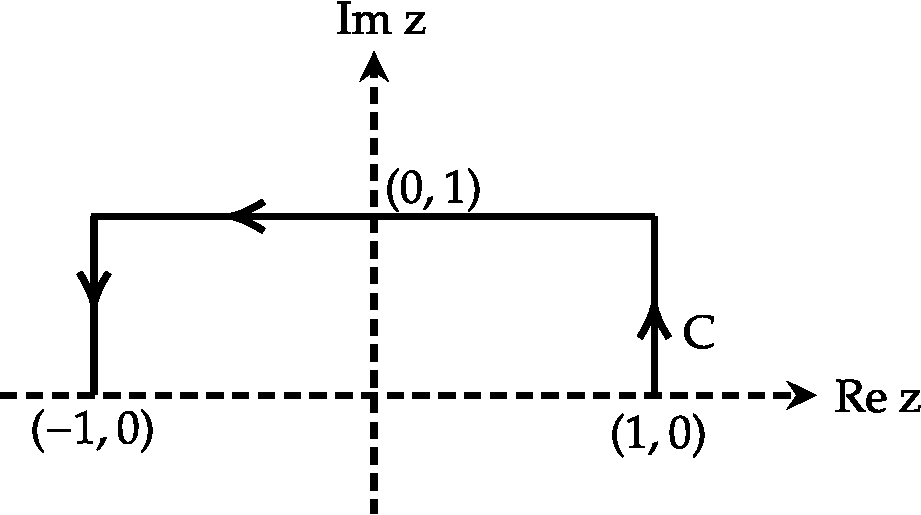
\includegraphics[height=5cm,width=9cm]{diagram-20211005-crop}
	\end{figure}
	\begin{tasks}(4)
		\task[\textbf{A.}] $\frac{5}{e}+e$
		\task[\textbf{B.}] $e-\frac{5}{e}$
		\task[\textbf{C.}] $\frac{5}{e}-e$
		\task[\textbf{D.}] $-\frac{5}{e}-e$
	\end{tasks}
	\begin{answer}
		\begin{align*}
		\intertext { If we complete the contour, then by Cauchy integral theorem }
		\int_{-1}^{1} d z z^{2} e^{z}+\int_{C} d z z^{2} e^{z}&=0 \Rightarrow \int_{C} d z z^{2} e^{z}=-\int_{-1}^{1} d z z^{2} e^{z}\\&=-\left[z^{2} e^{z}-2 z e^{2}+2 e^{2}\right]_{-1}^{1}=\frac{5}{e}-e
		\end{align*}
		So the correct answer is \textbf{Option (C)}
	\end{answer}
	\item Which of the following is an analytic function of the complex variable $z=x+i y$ in the domain $|z|<2 ?$
	{\exyear{NET/JRF(JUNE-2011)}}
	\begin{tasks}(2)
		\task[\textbf{A.}] $(3+x-i y)^{7}$
		\task[\textbf{B.}] $(1+x+i y)^{4}(7-x-i y)^{3}$
		\task[\textbf{C.}] $(1-x-i y)^{4}(7-x+i y)^{3}$
		\task[\textbf{D.}] $(x+i y-1)^{1 / 2}$
	\end{tasks}
	\begin{answer}
		Put $z=x+i y .$ If $\bar{z}=x-i y$ appears in any of the expressions then that expression is non-analytic. For option (D) we have a branch point singularity as the power is $\frac{1}{2}$ which is fractional. Hence only option (B) is analytic.\\\\
		So the correct answer is \textbf{Option (B)}
	\end{answer}
	\item The first few terms in the Laurent series for $\frac{1}{(z-1)(z-2)}$ in the region $1 \leq|z| \leq 2$ and around $z=1$ is
	{\exyear{NET/JRF(JUNE-2012)}}
	\begin{tasks}(1)
		\task[\textbf{A.}] $\frac{1}{2}\left[1+z+z^{2}+\ldots\right]\left[1+\frac{z}{2}+\frac{z^{2}}{4}+\frac{z^{3}}{8}+\ldots .\right]$
		\task[\textbf{B.}] $\frac{1}{1-z}-z-(1-z)^{2}+(1-z)^{3}+\ldots .$
		\task[\textbf{C.}] $\frac{1}{\mathrm{z}^{2}}\left[1+\frac{1}{\mathrm{z}}+\frac{1}{\mathrm{z}^{2}}+\ldots .\right]\left[1+\frac{2}{\mathrm{z}}+\frac{4}{\mathrm{z}^{2}}+\ldots . .\right]$
		\task[\textbf{D.}]  $2(z-1)+5(z-1)^{2}+7(z-1)^{3}+\ldots$
	\end{tasks}
	\begin{answer}
		\begin{align*}
		\frac{1}{(z-1)(z-2)}&=\frac{1}{z-2}-\frac{1}{z-1}=\frac{1}{1-z}+\frac{1}{(z-1)-1}\\&=\frac{1}{1-z}-(1+(1-z))^{-1}\\
		&=\frac{1}{1-z}-\left[1+(1-z)+\frac{(-1)(-2)}{2 !}(1-z)^{2}+\frac{(-1)(-2)(-3)}{3 !}(1-z)^{3} \ldots\right]\\
		&=\frac{1}{1-z}-\left[z+(1-z)^{2}-(1-z)^{3}+\ldots . .\right]
		\end{align*}
		So the correct answer is \textbf{Option (B)}
	\end{answer}
	\item Let $u(x, y)=x+\frac{1}{2}\left(x^{2}-y^{2}\right)$ be the real part of analytic function $f(z)$ of the complex variable $z=x+i y$. The imaginary part of $f(z)$ is
	{\exyear{NET/JRF(JUNE-2012)}}
	\begin{tasks}(4)
		\task[\textbf{A.}] $y+x y$
		\task[\textbf{B.}] $x y$
		\task[\textbf{C.}] $y$
		\task[\textbf{D.}] $y^{2}-x^{2}$
	\end{tasks}
	\begin{answer}
		\begin{align*}
		u(x, y)&=x+\frac{1}{2}\left(x^{2}-y^{2}\right), v(x, y)=?\\
		\text{Check }\frac{\partial u}{\partial x}&=\frac{\partial v}{\partial y}\text{ and } \frac{\partial u}{\partial y}=-\frac{\partial v}{\partial x}\\
		\Rightarrow \frac{\partial u}{\partial x}&=\frac{\partial v}{\partial y}, \quad \frac{\partial v}{\partial y}=1+x, \\ v&=y+x y+f(x)\\
		\frac{\partial u}{\partial y}&=-\frac{\partial v}{\partial x} \Rightarrow \frac{\partial v}{\partial x}=+y, \\ v&=y x+f(y)\\
		y+x y+f(x)&=y x+f(y)\\
		\text{If }f(x)&=0\quad \quad
		f(y)=y\\
		v&=x y+y
		\end{align*}
		So the correct answer is \textbf{Option (A)}
	\end{answer}
	\item The value of the integral $\int_{C} \frac{z^{3} d z}{\left(z^{2}-5 z+6\right)}$, where $C$ is a closed contour defined by the equation $2|z|-5=0$, traversed in the anti-clockwise direction, is
	{\exyear{NET/JRF(DEC-2012)}}
	\begin{tasks}(4)
		\task[\textbf{A.}] $-16 \pi i$
		\task[\textbf{B.}] $16 \pi \mathrm{i}$
		\task[\textbf{C.}] $8 \pi i$
		\task[\textbf{D.}] $2 \pi i$
	\end{tasks}
	\begin{answer}
		\begin{align*}
		z^{2}-5 z+6&=0 \Rightarrow z^{2}-2 z-3 z+6\\&=0 \Rightarrow z(z-2)-3(z-2)=0 \Rightarrow z=3,2\\
		2|z|&=5 \Rightarrow|z|=2.5,\text{ only 2 will be inside.}\\
		\text{Residue }&=\left.(z-2) \frac{z^{3}}{(z-3)(z-2)}\right|_{z=2}=\frac{8}{2-3}\\&=-8 \Rightarrow \int \frac{z^{3} d z}{z^{2}-5 z+6}=2 \pi i(-8)=-16 \pi i
		\end{align*}
		So the correct answer is \textbf{Option (A)}
	\end{answer}
	\item  With $z=x+i y$, which of the following functions $f(x, y)$ is NOT a (complex) analytic function of $z$ ?
	{\exyear{NET/JRF(JUNE-2013)}}
	\begin{tasks}(1)
		\task[\textbf{A.}] $f(x, y)=(x+i y-8)^{3}\left(4+x^{2}-y^{2}+2 i x y\right)^{7}$
		\task[\textbf{B.}] $f(x, y)=(x+i y)^{7}(1-x-i y)^{3}$
		\task[\textbf{C.}] $f(x, y)=\left(x^{2}-y^{2}+2 i x y-3\right)^{5}$
		\task[\textbf{D.}] $f(x, y)=(1-x+i y)^{4}(2+x+i y)^{6}$
	\end{tasks}
	\begin{answer}
		\begin{align*}
		f(x, y)&=(1-x+i y)^{4}(2+x+i y)^{6}\\&=\{1-(x-i y)\}^{4}(2+x+i y)^{6}\\
		\text{Due to present of }\bar{z}&=(x-i y)
		\end{align*}
		So the correct answer is \textbf{Option (D)}
	\end{answer}
	\item  Which of the following functions cannot be the real part of a complex analytic function of $z=x+i y ?$
	{\exyear{NET/JRF(DEC-2013)}}
	\begin{tasks}(4)
		\task[\textbf{A.}] $x^{2} y$
		\task[\textbf{B.}]  $x^{2}-y^{2}$
		\task[\textbf{C.}] $x^{3}-3 x y^{2}$
		\task[\textbf{D.}] $3 x^{2} y-y-y^{3}$
	\end{tasks}
	\begin{answer}
		\begin{align*}
		\intertext{ Let $x^{2} y$ be real part of a complex function. Use Milne Thomson's method to write analytic complex function. The real part of that function should be (1) but that is not the case. So this cannot be real part of an analytic function. Also,}
		z^{2}&=(x+i y)^{2}=x^{2}-y^{2}+2 i x y,\text{ Real part option (2)}\\
		z^{3}&=(x+i y)^{3}=x^{3}-i y^{3}+3 i x y(x+i y)\\
		&=x^{3}-i y^{3}+3 i x^{2} y-3 x y^{2},\text{ Real part option (3)}
		\end{align*}
		So the correct answer is \textbf{Option (A)}
	\end{answer}
	\item  Given that the integral $\int_{0}^{\infty} \frac{d x}{y^{2}+x^{2}}=\frac{\pi}{2 y}$, the value of $\int_{0}^{\infty} \frac{d x}{\left(y^{2}+x^{2}\right)^{2}}$ is
	{\exyear{NET/JRF(DEC-2013)}}
	\begin{tasks}(4)
		\task[\textbf{A.}] $\frac{\pi}{y^{3}}$
		\task[\textbf{B.}] $\frac{\pi}{4 y^{3}}$
		\task[\textbf{C.}]  $\frac{\pi}{8 y^{3}}$
		\task[\textbf{D.}] $\frac{\pi}{2 y^{3}}$
	\end{tasks}
	\begin{answer}
		\begin{align*}
		\int_{0}^{\infty} \frac{d x}{\left(y^{2}+x^{2}\right)^{2}}&=\frac{1}{2} \int_{-\infty}^{\infty} \frac{d x}{\left(y^{2}+x^{2}\right)^{2}},\text{ pole is of }2^{\text {nd }}\text{ order at }x=i y,\text{ residue }=1 /\left(4 i y^{3}\right)\\
		\text{Integral }&=\left(\frac{1}{2}\right)(2 \pi i) \frac{1}{4 i y^{3}}=\frac{\pi}{\left(4 y^{3}\right)}
		\end{align*}
	\end{answer}
	\item If $C$ is the contour defined by $|z|=\frac{1}{2}$, the value of the integral
	$$
	\oint_{C} \frac{d z}{\sin ^{2} z}
	$$
	is
	{\exyear{NET/JRF(JUNE-2014)}}
	\begin{tasks}(4)
		\task[\textbf{A.}] $\infty$
		\task[\textbf{B.}] $2 \pi i$
		\task[\textbf{C.}] 0
		\task[\textbf{D.}] $\pi i$
	\end{tasks}
	\begin{answer}
		\begin{align*}
		f(z)&=\frac{1}{\sin ^{2} z} \quad\left(|z|=\frac{1}{2}\right)\\
		\sin z&=z-\frac{z^{3}}{\lfloor 3}+\frac{z^{5}}{\lfloor 5} \ldots . \Rightarrow \frac{1}{\sin ^{2} z}=\frac{1}{\left(z-\frac{z^{3}}{\frac{3}{3}}+\frac{z^{5}}{5} \cdots\right)^{2}}\\
		\Rightarrow \frac{1}{\sin ^{2} z}&=\frac{1}{z^{2}}\left[1-\frac{z^{2}}{\lfloor 3}+\frac{z^{4}}{\lfloor 5} \ldots .\right]^{-2} \Rightarrow \oint_{C} \frac{d z}{\sin ^{2} z}=0
		\end{align*}
		So the correct answer is \textbf{Option (C)}
	\end{answer}
	\item The principal value of the integral $\int_{-\infty}^{\infty} \frac{\sin (2 x)}{x^{3}} d x$ is
	{\exyear{NET/JRF(DEC-2014)}}
	\begin{tasks}(4)
		\task[\textbf{A.}] $-2 \pi$
		\task[\textbf{B.}]  $-\pi$
		\task[\textbf{C.}] $\pi$
		\task[\textbf{D.}]  $2 \pi$
	\end{tasks}
	\begin{answer}
		\begin{align*}
		\text{Let }f(z)&=\frac{e^{i 2 z}}{z^{3}}\\
		\lim _{2 \rightarrow 0}(z-0)^{3} f(z)&=\lim _{z \rightarrow 0}(z-0)^{3} \frac{e^{i 2 z}}{z^{3}}\\&=1(\text{ finite and }\neq 0) \Rightarrow z=0 \text{is pole of order 3} .\\
		\text{Residue }R&=\frac{1}{2 !} \lim _{z \rightarrow 0} \frac{d^{2}}{d z^{2}}\left[(z-0)^{3} \frac{e^{i 2 z}}{z^{3}}\right]=-2\\
		\Rightarrow \int_{-\infty}^{\infty} f(x) d x&=\pi i \Sigma R=\pi i(-2)=-2 \pi i \Rightarrow \operatorname{Im} .\text{ Part }\\&=-2 \pi \Rightarrow \int_{-\infty}^{\infty} f(x) d x=-2 \pi
		\end{align*}
		So the correct answer is \textbf{Option (A)}
	\end{answer}
	\item The Laurent series expansion of the function $f(z)=e^{2}+e^{1 / 2}$ about $z=0$ is given by
	{\exyear{NET/JRF(DEC-2014)}}
	\begin{tasks}(2)
		\task[\textbf{A.}] $\sum_{n=-\infty}^{\infty} \frac{z^{n}}{n !}$ for all $|z|<\infty$
		\task[\textbf{B.}] $\sum_{n=0}^{\infty}\left(z^{n}+\frac{1}{z^{n}}\right) \frac{1}{n !}$ only if $0<|z|<1$
		\task[\textbf{C.}] $\sum_{n=0}^{\infty}\left(z^{n}+\frac{1}{z^{n}}\right) \frac{1}{n !}$ for all $0<|z|<\infty$
		\task[\textbf{D.}]  $\sum_{n=-\infty}^{\infty} \frac{z^{n}}{n !}$ only if $|z|<1$
	\end{tasks}
	\begin{answer}
		\begin{align*}
		e^{z}&=\left(1+z+\frac{z^{2}}{2 !}+\ldots\right)=\sum_{n=0}^{\infty} \frac{z^{n}}{n !}\text{ and }e^{1 / z}\\&=1+\frac{1}{z}+\frac{1}{2 !} \frac{1}{z^{2}}+\ldots .=\sum_{n=0}^{\infty} \frac{1}{z^{n} n !}\\
		\Rightarrow f(z)&=\left(e^{z}+e^{1 / 2}\right)=\sum_{n=0}^{\infty}\left(z^{n}+\frac{1}{z^{n}}\right) \frac{1}{n !},\text{ for all }0<|z|<\infty
		\end{align*}
		So the correct answer is \textbf{Option (C)}
	\end{answer}
	\item Consider the function $f(z)=\frac{1}{z} \ln (1-z)$ of a complex variable $z=r e^{i \theta}(r \geq 0, \quad-\infty<\theta<\infty)$. The singularities of $f(z)$ are as follows:
	{\exyear{NET/JRF(DEC-2014)}}
	\begin{tasks}(1)
		\task[\textbf{A.}]  Branch points at $z=1$ and $z=\infty$; and a pole at $z=0$ only for $0 \leq \theta<2 \pi$
		\task[\textbf{B.}] Branch points at $z=1$ and $z=\infty$; and a pole at $z=0$ for all $\theta$ other than $0 \leq \theta<2 \pi$
		\task[\textbf{C.}] Branch points at $z=1$ and $z=\infty$; and a pole at $z=0$ for all $\theta$
		\task[\textbf{D.}] Branch points at $z=0, z=1$ and $z=\infty$.
	\end{tasks}
	\begin{answer}
		\begin{align*}
		\text{For }f(z)&=\frac{1}{z} \ln (1-z)=\frac{1}{z}\left(-z-\frac{z^{2}}{2}-\frac{z^{3}}{3}-\ldots . .\right)\\&=-1-\frac{z}{2}-\frac{z^{2}}{3}-\ldots .
		\intertext{There is no principal part and when $z \rightarrow 0, f(z)=-1 .$ So there is removable singularity at $z=0$. Also $z=1$ and $z=\infty$ is Branch point.}
		\end{align*}
		None of the above is correct
	\end{answer}
	\item  The value of integral $\int_{-\infty}^{\infty} \frac{d x}{1+x^{4}}$
	{\exyear{NET/JRF(JUNE-2015)}}
	\begin{tasks}(4)
		\task[\textbf{A.}] $\frac{\pi}{\sqrt{2}}$
		\task[\textbf{B.}] $\frac{\pi}{2}$
		\task[\textbf{C.}] $\sqrt{2} \pi$
		\task[\textbf{D.}] $2 \pi$
	\end{tasks}
	\begin{answer}
		\begin{align*}
		\int_{-\infty}^{\infty} \frac{d z}{1+z^{4}} \quad \because|z|=R\\
		\text{Now, pole }z&=e^{(2 n+1) \frac{\pi}{4}}\\
		n&=0, \quad \Rightarrow z_{0}=e^{\frac{i \pi}{4}}=\frac{1}{\sqrt{2}}+i \frac{1}{\sqrt{2}}, n\\&=2 \Rightarrow z_{2}=\frac{-1}{\sqrt{2}}-i \frac{1}{\sqrt{2}}\\
		n&=1 \Rightarrow z_{1}=e^{\frac{i 3 \pi}{4}}=\frac{-1}{\sqrt{2}}+i \frac{1}{\sqrt{2}}, n\\&=3 \Rightarrow z_{3}=+\frac{1}{\sqrt{2}}-i \frac{1}{\sqrt{2}}
		\intertext{only $z_{0}$ and $z_{1}$ lies in contour}
		\text{i.e., residue at }\left(z=e^{\frac{i \pi}{4}}\right)&=\frac{1}{4}\left(-\frac{1}{\sqrt{2}}-i \frac{1}{\sqrt{2}}\right)\\
		\text{residue at }\left(z=e^{\frac{i 3 \pi}{4}}\right)&=\frac{1}{4}\left(\frac{1}{\sqrt{2}}-i \frac{1}{\sqrt{2}}\right)\\
		\text{now }\int_{-\infty}^{\infty} \frac{d x}{x^{4}+1}&=2 \pi i \Sigma \operatorname{Re} S=\frac{\pi}{\sqrt{2}}
		\end{align*}
		So the correct answer is \textbf{Option (A)}
	\end{answer}
	\item  The function $\frac{Z}{\sin \pi z^{2}}$ of a complex variable $z$ has
	{\exyear{NET/JRF(DEC-2015)}}
	\begin{tasks}(1)
		\task[\textbf{A.}] A simple pole at 0 and poles of order 2 at $\pm \sqrt{n}$ for $n=1,2,3 \ldots$
		\task[\textbf{B.}] A simple pole at 0 and poles of order 2 at $\pm \sqrt{n}$ and $\pm i \sqrt{n}$ for $n=1,2,3 \ldots$
		\task[\textbf{C.}] Poles of order 2 at $\pm \sqrt{n}, n=0,1,2,3 \ldots$
		\task[\textbf{D.}] Poles of order 2 at $\pm n, n=0,1,2,3 \ldots$
	\end{tasks}
	\begin{answer}
		\begin{align*}
		f(z)&=\frac{z}{\sin \pi z^{2}}=\frac{z}{\pi z^{2} \frac{\sin \pi z^{2}}{\pi z^{2}}}\\
		\text{	at }z&=0,\text{ it is a simple pole since,} \lim _{z \rightarrow 0} \frac{\sin \pi z^{2}}{\pi z^{2}}=1\\
		\text{Also, }\sin \pi z^{2}&=\sin n \pi \Rightarrow \pi \mathrm{z}^{2}\\&=\pm n \pi, z=\pm \sqrt{n}, \pm i \sqrt{n}\\
		\lim _{z \rightarrow \sqrt{n}}&(z-\sqrt{n})^{2} \cdot \frac{z}{\sin \pi z^{2}}, \text{exists. So its pole of order 2}
		\end{align*}
		So the correct answer is \textbf{Option (B)}
	\end{answer}
	\item The value of the contour integral $\frac{1}{2 \pi i} \oint_{C} \frac{e^{4 z}-1}{\cosh (z)-2 \sinh (z)} d z$ around the unit circle $C$ traversed in the anti-clockwise direction, is
	{\exyear{NET/JRF(JUNE-2016)}}
	\begin{tasks}(4)
		\task[\textbf{A.}] 0
		\task[\textbf{B.}] 2
		\task[\textbf{C.}] $\frac{-8}{\sqrt{3}}$
		\task[\textbf{D.}] $-\tanh \left(\frac{1}{2}\right)$
	\end{tasks}
	\begin{answer}
		\begin{align*}
		f(z)&=\frac{e^{4 z}-1}{\cosh z-2 \sinh z}=\frac{e^{4 z}-1}{\frac{e^{2}+e^{-z}}{2}-\left(e^{z}-e^{-z}\right)}\\&=\frac{e^{42}-1}{-\frac{e^{z}}{2}+\frac{3}{2} e^{-z}}\\
		\Rightarrow f(z)&=\frac{2 e^{2}\left(e^{4 z}-1\right)}{\left(3-e^{2 z}\right)}=\frac{2\left(e^{5 z}-e^{z}\right)}{\left(3-e^{2 z}\right)}\\
		\text{For pole at }z&=z_{0}, 3-e^{2 \xi_{0}}=0 \Rightarrow e^{2 z_{0}}\\&=3 \Rightarrow z_{0}=\frac{\ln 3}{2}
		\intertext{It has simple pole at $z_{0}$}
		\operatorname{Re}\left(z_{0}\right)&=\lim _{z \rightarrow z_{0}}\left(z-z_{0}\right) f(z)=\lim _{2 \rightarrow z_{0}}\left(z-z_{0}\right) \frac{2\left(e^{5 z}-e^{2}\right)}{3-e^{22}}\\
		&=\lim _{z \rightarrow z_{0}} \frac{\left(z-z_{0}\right) \times 2\left(5 e^{5 z}-e^{z}\right)+2\left(e^{5 z}-e^{z}\right) \times 1}{-2 e^{2 z}}\\&=-\left(\frac{e^{5 z_{0}}-e^{z_{0}}}{e^{2 z_{0}}}\right)\\
		&=-\left(\frac{(\sqrt{3})^{5}-\sqrt{3}}{3}\right)=-\left(\frac{9 \sqrt{3}-\sqrt{3}}{3}\right)=-\frac{8}{\sqrt{3}}\\
		\frac{1}{2 \pi i} \oint f(z) d z&=\frac{1}{2 \pi i} \times 2 \pi i \sum\text{ Residue } =-\frac{8}{\sqrt{3}}
		\end{align*}
		So the correct answer is \textbf{Option (C)}
	\end{answer}
	\item  Let $u(x, y)=e^{a x} \cos (b y)$ be the real part of a function $f(z)=u(x, y)+i v(x, y)$ of the complex variable $z=x+i y$, where $a, b$ are real constants and $a \neq 0 .$ The function $f(z)$ is complex analytic everywhere in the complex plane if and only if
	{\exyear{NET/JRF(JUNE-2017)}}
	\begin{tasks}(4)
		\task[\textbf{A.}] $b=0$
		\task[\textbf{B.}] $b=\pm a$
		\task[\textbf{C.}] $b=\pm 2 \pi a$
		\task[\textbf{D.}]  $b=a \pm 2 \pi$
	\end{tasks}
	\begin{answer}
		\begin{align*}
		\intertext{The function $f(z)$ will be analytic everywhere in the complex plane if and only if it satisfies the Cauchy Riemann equation in that region.}
		\Rightarrow \frac{\partial u}{\partial x}&=\frac{\partial v}{\partial y}\text{ and } \frac{\partial u}{\partial y}=-\frac{\partial v}{\partial x}\\
		\text{Hence }a e^{a x} \cos (b y)&=\frac{\partial v}{\partial y}\hspace{2cm}\text{(i)}\\
		\text{and }b e^{a x} \sin (b y)&=\frac{\partial v}{\partial x}\hspace{2cm}\text{(ii)}
		\intertext{From equation (i)}
		v(x, y)&=\frac{a e^{a x} \sin (b y)}{b}+c(y)\hspace{2cm}\text{(iii)}
		\intertext{Differentiating partially with $x$ gives}
		\frac{\partial v}{\partial x}&=\frac{a^{2} e^{a x} \sin (b y)}{b}\hspace{2cm}\text{(iv)}
		\intertext{From equation (iii) and (iv)}
		b e^{a x} \sin (b y)&=\frac{a^{2} e^{a x} \sin (b y)}{b}\\
		\Rightarrow b^{2}&=a^{2} \Rightarrow b=\pm a
		\end{align*}
		So the correct answer is \textbf{Option (B)}
	\end{answer}
	\item  The integral $\oint_{\Gamma} \frac{z e^{i \pi z / 2}}{z^{2}-1} d z$ along the closed contour $\Gamma$ shown in the figure is
	{\exyear{NET/JRF(JUNE-2017)}}
	\begin{figure}[H]
		\centering
		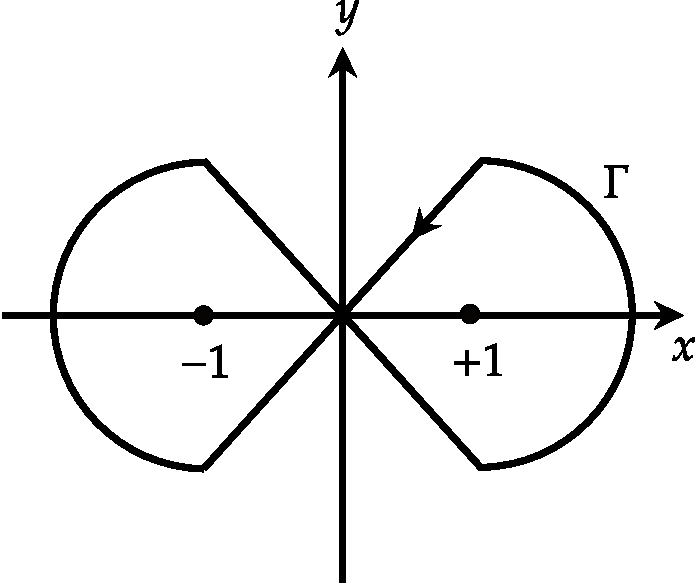
\includegraphics[height=4cm,width=5cm]{diagram-20211005(19)-crop}
	\end{figure}
	\begin{tasks}(4)
		\task[\textbf{A.}] 0
		\task[\textbf{B.}] $2 \pi$
		\task[\textbf{C.}] $-2 \pi$
		\task[\textbf{D.}] $4 \pi i$
	\end{tasks}
	\begin{answer}
		\begin{align*}
		f(z)&=\frac{z e^{i z \pi / 2}}{(z+1)(z-1)}\\
		\text{For }z&=+1\text{ anti-clockwise}\\
		I&=2 \pi i \lim _{z \rightarrow 1} \frac{z e^{i \pi z / 2}}{(z+1)}=\frac{2 \pi i}{2} e^{i \pi / 2}=\pi i e^{i \pi / 2}\\
		\text{For }z&=-1\\
		I&=-2 \pi i \lim _{z \rightarrow-1} \frac{z e^{i \pi z / 2}}{(z-1)}=-2 \pi i \times \frac{(-1) e^{-i \pi / 2}}{(-2)}=-\pi i e^{-i \pi / 2}\\
		\text{Integral }&=\pi i \frac{\left(e^{i \pi / 2}-e^{-i \pi / 2}\right)}{2 i} \times 2 i=2 \pi i^{2} \sin \frac{\pi}{2}=-2 \pi
		\end{align*}
		So the correct answer is \textbf{Option (C)}
	\end{answer}
	\item What is the value of $a$ for which $f(x, y)=2 x+3\left(x^{2}-y^{2}\right)+2 i(3 x y+a y)$ is an analytic function of complex variable $z=x+i y$
	{\exyear{NET/JRF(JUNE-2018)}}
	\begin{tasks}(4)
		\task[\textbf{A.}] 1
		\task[\textbf{B.}] 0
		\task[\textbf{C.}] 3
		\task[\textbf{D.}] 2
	\end{tasks}
	\begin{answer}
		\begin{align*}
		f(x, y)&=2 x+3\left(x^{2}-y^{2}\right)+2 i(3 x y+\alpha y)\\
		u&=2 x+3\left(x^{2}-y^{2}\right), v=2(3 x y+\alpha y)\\
		\text{C-R conditions: }u_{x}&=v_{y}, u_{y}=-v_{x}\\
		2+3(2 x)&=2(3 x+\alpha) \Rightarrow \alpha=1 \Rightarrow-6 y=-6 y
		\end{align*}
		So the correct answer is \textbf{Option (A)}
	\end{answer}
	\item  The value of the integral $\oint_{C} \frac{d z}{z} \frac{\tanh 2 z}{\sin \pi z}$, where $C$ is a circle of radius $\frac{\pi}{2}$, traversed counter-clockwise, with centre at $z=0$, is
	{\exyear{NET/JRF(DEC-2018)}}
	\begin{tasks}(4)
		\task[\textbf{A.}] 4
		\task[\textbf{B.}] $4 i$
		\task[\textbf{C.}] $2 i$
		\task[\textbf{D.}] 0
	\end{tasks}
	\begin{answer}$\left. \right. $
		\begin{figure}[H]
			\centering
			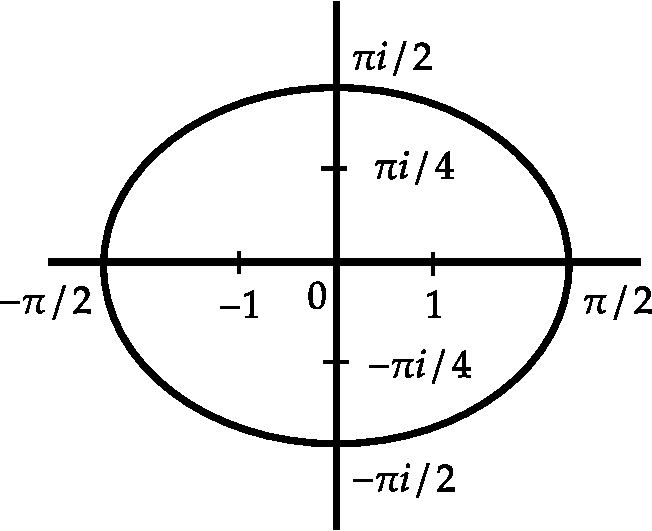
\includegraphics[height=4.5cm,width=5.5cm]{diagram-20211005(2)-crop}
		\end{figure}
		\begin{align*}
		&\oint_{C} \frac{d z}{z} \frac{\tanh 2 z}{\sin \pi z} d z\\
		z&=0,1,-1, \frac{\pi i}{4}, \frac{-\pi i}{4}\\
		f(z)&=\frac{2 z-\frac{1}{3}(2 z)^{3}+\frac{2}{15}(2 z)^{5} \ldots .}{z\left(\pi z-\frac{\pi^{3} z^{3}}{3 !}+\ldots\right)}\\
		\frac{2}{\pi z}&\left(1-\frac{1}{2} z^{2}+\ldots\right)\left(1-\frac{\pi^{2} z^{2}}{2 !}+\ldots\right)\\
		b_{1}&=\frac{2}{\pi}\\
		\text{As Re } z&=1, \frac{\tanh ^{2}}{-\pi}\text{ and }\operatorname{Re} z=-1, \frac{\tanh ^{2}}{-\pi}\\
		\operatorname{Re} z&=\frac{i \pi}{4}=-\frac{1}{\pi}\left(2 \operatorname{cosec} h \frac{\pi^{2}}{4}\right)\\
		\operatorname{Re} z&=\frac{-i \pi}{4}=-\frac{1}{\pi}\left(2 \operatorname{cosec} \mathrm{h} \frac{\pi^{2}}{4}\right)
		\intertext{$I=2 \pi i \Sigma R=4 i$ only when 0 lies inside, otherwise wrong question.}
		\end{align*}
		So the correct answer is \textbf{Option (B)}
	\end{answer}
	\item The integral $I=\int_{C} e^{z} d z$ is evaluated from the point $(-1,0)$ to $(1,0)$ along the contour $C$, which is an arc of the parabola $y=x^{2}-1$, as shown in the figure. The value of $I$ is
	{\exyear{NET/JRF(DEC-2018)}}
	\begin{figure}[H]
		\centering
		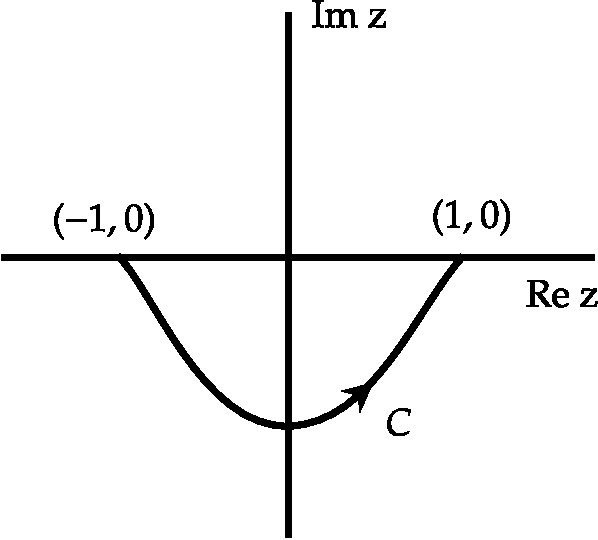
\includegraphics[height=4.5cm,width=5cm]{diagram-20211005(3)-crop}
	\end{figure}
	\begin{tasks}(4)
		\task[\textbf{A.}]  0
		\task[\textbf{B.}] $2 \sinh 1$
		\task[\textbf{C.}]  $e^{2 i} \sinh 1$
		\task[\textbf{D.}] $e+e^{-1}$
	\end{tasks}
	\begin{answer}
		\begin{align*}
		\int_{C} f(z) d z&=2 \pi i \Sigma R\\
		\int_{C} f(z) d z+\int_{1}^{-1} e^{x} d x&=0\\
		\int_{C} f(z) d z&=-\int_{1}^{-1} e^{x} d x=\int_{1}^{-1} e^{x} d x\\&=\frac{\left(e^{1}-e^{-1}\right)}{2} \cdot 2=2 \sinh 1
		\end{align*}
		So the correct answer is \textbf{Option (B)}
	\end{answer}
	\item The contour $C$ of the following integral
	$$
	\oint_{C} d z \frac{\sqrt{(z-1)(z-3)}}{\left(z^{2}-25\right)^{3}}
	$$
	in the complex $z$ plane is shown in the figure below.\\
	\begin{figure}[H]
		\centering
		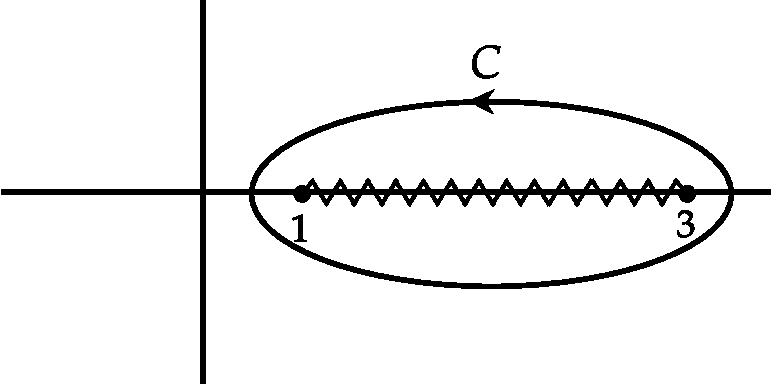
\includegraphics[height=3.5cm,width=6cm]{diagram-20211005(8)-crop}
	\end{figure}
	This integral is equivalent to an integral along the contours
	{\exyear{NET/JRF(DEC-2018)}}
	\begin{tasks}(2)
		\task[\textbf{A.}] \begin{figure}[H]
			\centering
			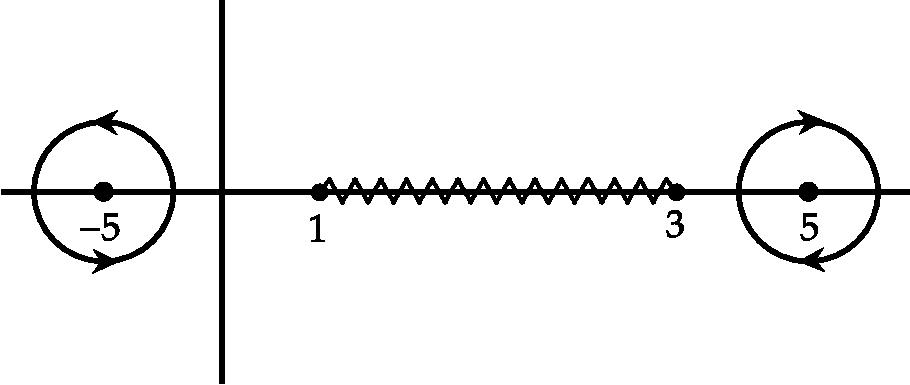
\includegraphics[height=3cm,width=6.5cm]{diagram-20211005(4)-crop}
		\end{figure}
		\task[\textbf{B.}] \begin{figure}[H]
			\centering
			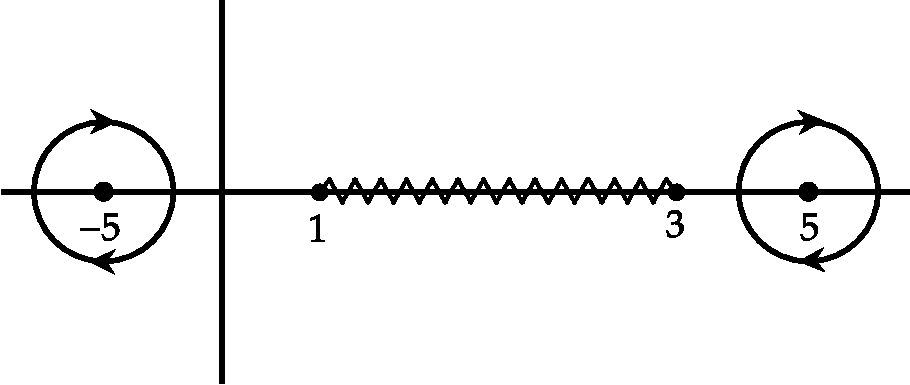
\includegraphics[height=3cm,width=6.5cm]{diagram-20211005(5)-crop}
		\end{figure}
		\task[\textbf{C.}] \begin{figure}[H]
			\centering
			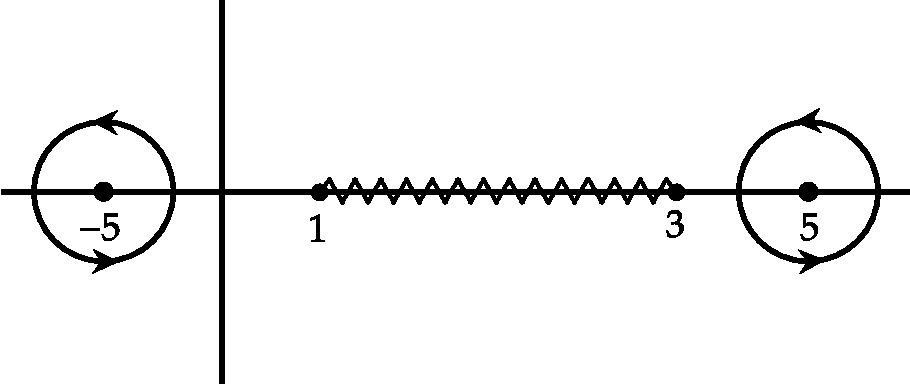
\includegraphics[height=3cm,width=6.5cm]{diagram-20211005(6)-crop}
		\end{figure}
		\task[\textbf{D.}] \begin{figure}[H]
			\centering
			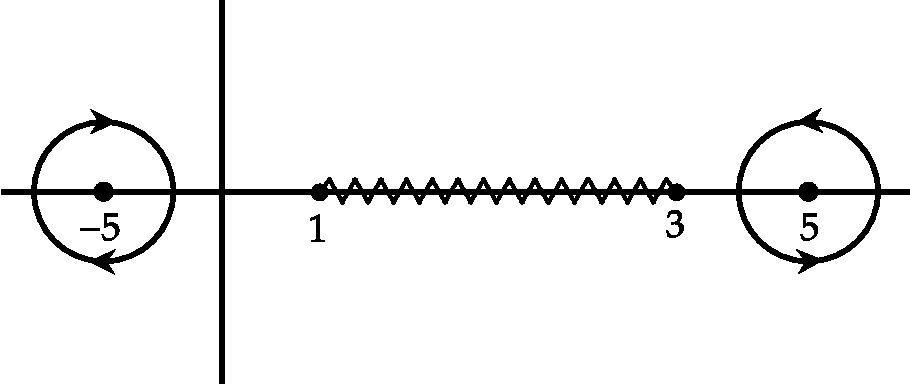
\includegraphics[height=3cm,width=6.5cm]{diagram-20211005(7)-crop}
		\end{figure}
	\end{tasks}
	\begin{answer}
		\begin{align*}
		\intertext{$z=1,3$ are branch points $\infty$ is not a branch point 1 branch cut 3}
		\end{align*}
		So the correct answer is \textbf{Option (C)}
	\end{answer}
	\item  Let $C$ be the circle of radius $\frac{\pi}{4}$ centered at $z=\frac{1}{4}$ in the complex $z$-plane that is traversed counter-clockwise. The value of the contour integral $\oint_{C} \frac{z^{2}}{\sin ^{2} 4 z} d z$ is
	{\exyear{NET/JRF(DEC-2019)}}
	\begin{tasks}(4)
		\task[\textbf{A.}] 0
		\task[\textbf{B.}] $\frac{i \pi^{2}}{4}$
		\task[\textbf{C.}] $\frac{i \pi^{2}}{16}$
		\task[\textbf{D.}] $\frac{i \pi}{4}$
	\end{tasks}
	\begin{answer}$\left. \right. $
		\begin{figure}[H]
			\centering
			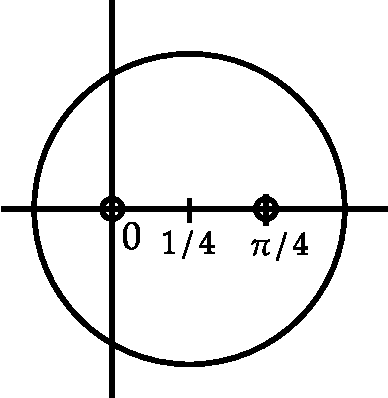
\includegraphics[height=3cm,width=3cm]{diagram-20211026(16)-crop}
		\end{figure}
		\begin{align*}
		f(z)&=\left(\frac{\pi}{\sin 4 z}\right)^{2}\\
		z_{0}&=0, \frac{\pi}{4}\text{ are poles}\\
		4 z&=n \pi, z=0, \frac{\pi}{4}
		\intertext{Others are outside the contour.}
		\text{Residue at }z&=0\text{ is }\left[\frac{\pi}{4 z-\frac{4^{3} z^{3}}{3 !}+\ldots}\right]^{2}\\
		&=\left[\frac{1}{4-\frac{4^{3} z^{2}}{3 !}+\ldots .}\right]^{2}\qquad \text{ No terms for } \frac{1}{z}, b_{1}=0\\
		&=\left[4-\frac{4^{3} z^{2}}{3 !}+\ldots .\right]^{-2}\\
		\text{Residue for }z&=\frac{\pi}{4}\\
		z-\frac{\pi}{4}&=t
		\intertext{$\sin (4 t+\pi)=-\sin 4 t \quad$ (But square so no effect)}
		&\left[\frac{t+\frac{\pi}{4}}{\sin 4\left(t+\frac{\pi}{4}\right)}\right]^{2}\\
		\left(\frac{t+\frac{\pi}{4}}{\sin 4 t}\right)^{2}&=\frac{t^{2}+\frac{\pi^{2}}{4}+2 t \cdot \frac{\pi}{4}}{\sin ^{2} 4 t}\\
		\frac{\pi}{2} \frac{t}{16 t^{2}[1-\ldots .]^{2}}&=\frac{\pi}{32 t}[1-\ldots .]^{-2} \text{(from first term)}\\
		b_{1}&=\frac{\pi}{32}\\
		\oint_{C} \frac{z^{2}}{\sin ^{2} 4 z} d z&=2 \pi i\left[0+\frac{\pi}{32}\right]=\frac{i \pi^{2}}{16}
		\end{align*}
		So the correct answer is \textbf{Option (C)}
	\end{answer}
	\item  A function of a complex variable $z$ is defined by the integral $f(z)=\oint_{\Gamma} \frac{w^{2}-2}{w-z} d w$, where $\Gamma$ is a circular contour of radius 3 , centred at origin, running counter-clockwise in the $w$ - plane. The value of the function at $z=(2-i)$ is
	{\exyear{NET/JRF(JUNE-2020)}}
	\begin{tasks}(4)
		\task[\textbf{A.}] 0
		\task[\textbf{B.}] $1-4 i$
		\task[\textbf{C.}]  $8 \pi+2 \pi \mathrm{i}$
		\task[\textbf{D.}] $-\frac{2}{\pi}-\frac{i}{2 \pi}$
	\end{tasks}
	\begin{answer}$\left. \right. $
		\begin{figure}[H]
			\centering
			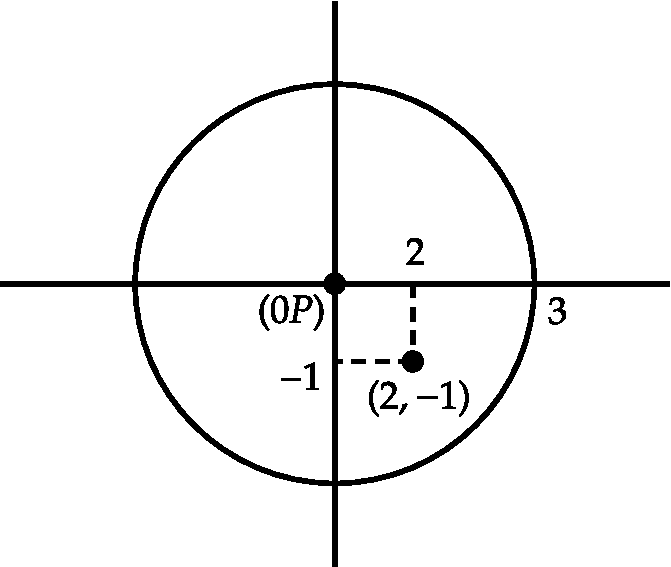
\includegraphics[height=4cm,width=4.6cm]{diagram-20211027-crop}
		\end{figure}
		\begin{align*}
		f(z)&=\oint_{\Gamma} \frac{w^{2}-2}{w-z} d w\\
		\omega&=z\text{ is a simple pole.}\\
		\text{Residue }\lim _{\omega \rightarrow z}(\omega-z) \frac{\left(\omega^{2}-2\right)}{(\omega-z)}&=(2-i)^{2}-2 \\&=4-1-4 i-2=(1-4 i)\\
		f(z)&=\oint_{\Gamma} \frac{w^{2}-2}{w-z} d w=2 \pi i(1-4 i)=2 \pi i+8 \pi
		\end{align*}
		So the correct answer is \textbf{Option (C)}
	\end{answer}
\end{enumerate}
\colorlet{ocre1}{ocre!70!}
\colorlet{ocrel}{ocre!30!}
\setlength\arrayrulewidth{1pt}
\begin{table}[H]
	\centering
	\arrayrulecolor{ocre}
	\begin{tabular}{|p{1.5cm}|p{1.5cm}||p{1.5cm}|p{1.5cm}|}
		\hline
		\multicolumn{4}{|c|}{\textbf{Answer key}}\\\hline\hline
		\rowcolor{ocrel}Q.No.&Answer&Q.No.&Answer\\\hline
		1&\textbf{C} &2&\textbf{B}\\\hline 
		3&\textbf{B} &4&\textbf{A} \\\hline
		5&\textbf{A} &6&\textbf{D} \\\hline
		7&\textbf{A}&8&\textbf{-}\\\hline
		9&\textbf{C}&10&\textbf{A}\\\hline
		11&\textbf{C} &12&\textbf{-}\\\hline
		13&\textbf{A}&14&\textbf{B}\\\hline
		15&\textbf{C}&16&\textbf{B}\\\hline
		17&\textbf{C} &18&\textbf{A}\\\hline
		19&\textbf{B}&20&\textbf{B}\\\hline
		21&\textbf{C}&22&\textbf{C}\\\hline
		23&\textbf{C}& &\\\hline
		
	\end{tabular}
\end{table}
\newpage
\begin{abox}
	Practise Set-2
\end{abox}
\begin{enumerate}[label=\color{ocre}\textbf{\arabic*.}]
	\item  The value of the integral $\oint_{C} \frac{e^{z} \sin (z)}{z^{2}} d z$, where the contour $C$ is the unit circle: $|z-2|=1$, is
	{\exyear{GATE 2010}}
	\begin{tasks}(4)
		\task[\textbf{A.}] $2 \pi i$
		\task[\textbf{B.}] $4 \pi i$
		\task[\textbf{C.}] $\pi i$
		\task[\textbf{D.}] 0
	\end{tasks}
	\begin{answer}
		\begin{align*}
		\intertext{$|z-2|=1 \Rightarrow 1<z<3$ i.e. the pole $z=0$ does not lie inside the contour.}
		\therefore \quad \oint_{C} \frac{e^{z} \sin z}{z^{2}} d z=2 \pi i \times 0=0 .
		\end{align*}
		So the correct answer is \textbf{Option (D)}
	\end{answer}
	\item Which of the following statements is TRUE for the function $f(z)=\frac{z \sin z}{(z-\pi)^{2}}$ ?
	{\exyear{GATE 2011}}
	\begin{tasks}(1)
		\task[\textbf{A.}] $f(z)$ is analytic everywhere in the complex plane
		\task[\textbf{B.}] $f(z)$ has a zero at $z=\pi$
		\task[\textbf{C.}] $f(z)$ has a pole of order 2 at $z=\pi$
		\task[\textbf{D.}] $f(z)$ has a simple pole at $z=\pi$
	\end{tasks}
	\begin{answer}
		\begin{align*}
		f(z)=\frac{z \sin z}{(z-\pi)^{2}}\text{ has a pole of order 2 at }z=\pi
		\end{align*}
		So the correct answer is \textbf{Option (C)}
	\end{answer}
	\item For the function $f(z)=\frac{16 z}{(z+3)(z-1)^{2}}$, the residue at the pole $z=1$ is (your answer should be an integer)-------
	{\exyear{GATE 2013}}
	\begin{answer}
		\begin{align*}
		\text{	At }z&=1,\text{ pole is of order 2 .} \\&\text{So, residue is }\frac{1}{\lfloor-1} \frac{d^{2-1}}{d z^{2-1}}\left[\frac{(z-1)^{2} 16 z}{(z+3)(z-1)^{2}}\right]_{z=1}=3
		\end{align*}
	\end{answer}
	\item The value of the integral
	$$
	\oint_{C} \frac{z^{2}}{e^{z}+1} d z
	$$
	where $C$ is the circle $|z|=4$, is
	{\exyear{GATE 2014}}
	\begin{tasks}(4)
		\task[\textbf{A.}] $2 \pi i$
		\task[\textbf{B.}] $2 \pi^{2} i$
		\task[\textbf{C.}]  $4 \pi^{3} i$
		\task[\textbf{D.}] $4 \pi^{2} i$
	\end{tasks}
	\begin{answer}
		\begin{align*}
		\text{	Pole }e^{z}&=-1 \Rightarrow e^{z}=e^{i(2 m+1) \pi}\text{ where }m=0,1,2,3 \ldots \ldots\\
		\text{For }z&=i \pi,\text{ Res }=\lim _{z=i \pi} \frac{\phi(z)}{\phi^{\prime}(z)}\\&=-\frac{\pi^{2}}{e^{i \pi}}=\pi^{2}\\
		\text{Similarly, for }z&=-i \pi,\text{ Res }=\pi^{2}\\
		\therefore I&=2 \pi i\left(\pi^{2}+\pi^{2}\right)=4 \pi^{3} i
		\end{align*}
			So the correct answer is \textbf{Option (C)}
	\end{answer}
	\item Consider a complex function $f(z)=\frac{1}{z\left(z+\frac{1}{2}\right) \cos (z \pi)}$. Which one of the following statements is correct?
	{\exyear{GATE 2015}}
	\begin{tasks}(1)
		\task[\textbf{A.}] $f(z)$ has simple poles at $z=0$ and $z=-\frac{1}{2}$
		\task[\textbf{B.}] $f(z)$ has second order pole at $z=-\frac{1}{2}$
		\task[\textbf{C.}] $f(z)$ has infinite number of second order poles
		\task[\textbf{D.}] $f(z)$ has all simple poles
	\end{tasks}
	\begin{answer}
		\begin{align*}
		f(z)&=\frac{1}{z\left(z+\frac{1}{2}\right) \cos (z \pi)}\\
		\text{	For $n^{t h}$ order pole, Res. }&=\lim _{z \rightarrow a}(z-a)^{n} f(z)=\text{ finite}\\
		\text{At }z&=0, \lim _{z \rightarrow 0} z f(z)=\text{ finite }\\\Rightarrow z&=0\text{ is a simple pole.}\\
		\text{At }z&=-\frac{1}{2}, \lim _{z \rightarrow-\frac{1}{2}} \frac{\left(z+\frac{1}{2}\right)^{2}}{z\left(z+\frac{1}{2}\right) \cos z \pi}=\lim _{z \rightarrow-\frac{1}{2}} \frac{\left(z+\frac{1}{2}\right)}{z \cos z \pi}\\&=\lim _{z \rightarrow-\frac{1}{2}} \frac{1}{1 . \cos z \pi+z . \pi(-\sin z \pi)}\\
		&=\lim _{z \rightarrow-\frac{1}{2}} \frac{1}{\cos z \pi-z \pi \sin z \pi}=\frac{1}{-\frac{\pi}{2}}\\&=-\frac{2}{\pi}=\text{ finite}\\
		\Rightarrow f(z)\text{ has second order pole at }z&=-\frac{1}{2}
		\end{align*}
		So the correct answer is \textbf{Option (A)}
	\end{answer}
	\item  Consider $w=f(z)=u(x, y)+i v(x, y)$ to be an analytic function in a domain $D$. Which one of the following options is NOT correct?
	{\exyear{GATE 2015}}
	\begin{tasks}(1)
		\task[\textbf{A.}] $u(x, y)$ satisfies Laplace equation in D
		\task[\textbf{B.}]  $v(x, y)$ satisfies Laplace equation in $D$
		\task[\textbf{C.}] $\int_{1}^{z_{2}} f(z) d z$ is dependent on the choice of the contour between $z_{1}$ and $z_{2}$ in $D$
		\task[\textbf{D.}]  $f(z)$ can be Taylor expended in $D$
	\end{tasks}
	\begin{answer}
		\begin{align*}
		w&=f(z)=u(x, y)+i v(x, y)\text{ to be an analytic function in a domain }D, \int_{z_{1}}^{z_{2}} f(z) d z\text{ is}\\
		&\text{independent of the choice of the contour between }z_{1}\text{ and }z_{2}\text{ in }D.
		\end{align*}
		So the correct answer is \textbf{Option (C)}
	\end{answer}
	\item A function $y(z)$ satisfies the ordinary differential equation $y^{\prime \prime}+\frac{1}{z} y^{\prime}-\frac{m^{2}}{z^{2}} y=0$, where\\
	$m=0,1,2,3, \ldots . .$ Consider the four statements P, Q, R, S as given below.\\
	$\mathrm{P}: z^{m}$ and $z^{-m}$ are linearly independent solutions for all values of $m$\\
	Q: $z^{m}$ and $z^{-m}$ are linearly independent solutions for all values of $m>0$\\
	$\mathrm{R}$ : $\ln z$ and 1 are linearly independent solutions for $m=0$\\
	S: $z^{m}$ and $\ln z$ are linearly independent solutions for all values of $m$\\
	The correct option for the combination of valid statements is
	{\exyear{GATE 2015}}
	\begin{tasks}(4)
		\task[\textbf{A.}] P, R and S only
		\task[\textbf{B.}]  P and R only
		\task[\textbf{C.}] $\mathrm{Q}$ and $\mathrm{R}$ only
		\task[\textbf{D.}] $\mathrm{R}$ and $\mathrm{S}$ only
	\end{tasks}
	\begin{answer}
		\begin{align*}
		y^{\prime \prime}+\frac{1}{z} y^{\prime}-\frac{m^{2}}{z^{2}} y&=0 \Rightarrow z^{2} y^{\prime \prime}+z y^{\prime}-m^{2} y\\&=0, m=0,1,2,3, \ldots, \quad z=e^{x}, D=\frac{d}{d x}\\
		\text{	If }m&=0 ; \quad z^{2} y^{\prime \prime}+z y^{\prime}=0,[D(D-1)+D] y\\&=0 \Rightarrow\left[D^{2}-D+D\right] y=0\\
		D^{2} y&=0 \Rightarrow y=c_{1}+c_{2} x \Rightarrow y\\&=c_{1}+c_{2} \ln z \quad \text{( $R$ is correct)}\\
		\text{And if }m &\neq 0, m>0,\text{ then }m \neq 0,\text{ then }\left(D^{2}-m^{2}\right) y\\&=0 \Rightarrow D=\pm m\\
		y&=c_{1} e^{m x}+c_{2} e^{-m x}=c_{1} e^{m \log z}+c_{2} e^{-m \log z}\\&=c_{1} z^{m}+c_{2} z^{-m}\\
		\text{or if }m &\neq 0, m>0,\text{ then}\\
		y&=c_{1} \cosh (m \log (z))+i c_{2} \sinh (m \log (x)), \quad m>0
		\end{align*}
		So the correct answer is \textbf{Option (C)} 
	\end{answer}
	\item  Which of the following is an analytic function of $z$ everywhere in the complex plane?
	{\exyear{GATE 2016}}
	\begin{tasks}(4)
		\task[\textbf{A.}] $z^{2}$
		\task[\textbf{B.}]  $\left(z^{*}\right)^{2}$
		\task[\textbf{C.}] $|z|^{2}$
		\task[\textbf{D.}] $\sqrt{z}$
	\end{tasks}
	\begin{answer}
		\begin{align*}
		z^{2}&=(x+i y)^{2}=x^{2}-y^{2}+i(2 x y) \Rightarrow u\\&=x^{2}-y^{2}\text{ and }v=2 x y\\
		\text{Cauchy Riemann equations }\frac{\partial u}{\partial x}&=\frac{\partial v}{\partial y}=2 x, \quad \frac{\partial v}{\partial x}=-\frac{\partial u}{\partial y}=2 y\text{ satisfies.}
		\end{align*}
		So the correct answer is \textbf{Option (A)}
	\end{answer}
	\item The contour integral $\oint \frac{d z}{1+z^{2}}$ evaluated along a contour going from $-\infty$ to $+\infty$ along the
	real axis and closed in the lower half-plane circle is equal to............... (up to two decimal places).
	{\exyear{GATE 2017}}
	\begin{answer}
		\begin{align*}
		\oint_{c} \frac{1}{1+z^{2}} d z&=\int_{-\infty}^{+\infty} \frac{1}{1+x^{2}} d x+\oint_{c} \frac{1}{1+z^{2}} d z\\
		\text{Poles, }1+z^{2}&=0 \Rightarrow z=\pm i, \quad z=-i\text{ is inside }C\\
		\therefore \operatorname{Res}(z=-i)&=\lim _{z \rightarrow-i}(z+i) \frac{1}{(z-i)(z+i)}\\&=\frac{1}{-i-i}=\frac{1}{-2 i}\\
		\int_{-\infty}^{+\infty} \frac{1}{1+x^{2}} d x&=-\frac{1}{2 i} \times-2 \pi i=\pi
		\intertext{(Since, here we use lower half plane i.e., we traversed in clockwise direction, hence we have to take $-2 \pi i$ )}
		\end{align*}
	\end{answer}
	\item The imaginary part of an analytic complex function is $v(x, y)=2 x y+3 y .$ The real part of the function is zero at the origin. The value of the real part of the function at $1+i$ is ................. (up to two decimal places)
	{\exyear{GATE 2017}}
	\begin{answer}
		\begin{align*}
		\intertext{Solution: The imaginary part of the given analytic function is $v(x, y)=2 x y+3 y .$ From the
			Cauchy - Riemann condition}
		\frac{\partial v}{\partial y}&=\frac{\partial u}{\partial x}=2 x+3
		\intertext{Integrating partially gives}
		u(x, y)&=x^{2}+3 x+g(y)\\
		\intertext{From the second Cauchy - Riemann condition}
		\frac{\partial u}{\partial y}&=-\frac{\partial v}{\partial x},\text{ we obtain} \frac{\partial u}{\partial y}\\&=-2 y, \mu(x, y)=-y^{2}+g(x)\\
		\frac{d g(y)}{d y}&=-2 y \Rightarrow g(y)=-y^{2}+c\\
		\text{	Hence, }u(x, y)&=x^{2}+3 x-y^{2}+c
		\intertext{Since, the real part of the analytic function is zero at the origin.}
		\text{Hence, }0&=0+0-0+c \Rightarrow c=0\\
		\text{Thus, }u(x, y)&=x^{2}+3 x-y^{2}\\
		\therefore f(z)&=\left(x^{2}+3 x-y^{2}\right)+i(2 x y+3 y)
		\intertext{Thus, the value of real part when}
		z&=1+i, i.e. x=1\text{ and }y=1\text{ is }u(x, y)\\&=(1)^{2}+3(1)-1=3
		\end{align*}
	\end{answer}
	\item The absolute value of the integral
	$$
	\int \frac{5 z^{3}+3 z^{2}}{z^{2}-4} d z
	$$
	over the circle $|z-1.5|=1$ in complex plane, is $\ldots$ (up to two decimal places).
	{\exyear{GATE 2018}}
	\begin{answer}
		\begin{align*}
		f(z)&=\frac{5 z^{3}+3 z^{2}}{(z-2)(z+2)}\\
		\text{Pole, }z&=2,-2\\
		z&=-2 \text{ is outside the center}\\
		|-2-1.5|>1&\text{So, will not be considered}\\
		\text{	Now, }\operatorname{Re} s(2)&=\lim _{z \rightarrow 2}(z-2) \frac{\left(5 z^{3}+3 z^{2}\right)}{(z-2)(z+2)}\\&=\frac{52^{3}+32^{2}}{4}=\frac{40+12}{4}=13\\
		I&=2 \pi i \times residue =2 \pi i \times 13\\&=26 \times 3.14 \Rightarrow I=81.64
		\end{align*}
	\end{answer}
	\item The pole of the function $f(z)=\cot z$ at $z=0$ is
	{\exyear{GATE 2019}}
	\begin{tasks}(2)
		\task[\textbf{A.}] A removable pole
		\task[\textbf{B.}] An essential singularity
		\task[\textbf{C.}]  A simple pole
		\task[\textbf{D.}] A second order pole
	\end{tasks}
	\begin{answer}
		\begin{align*}
		f(z)&=\cot z\text{ at }z=0\\
		f(z)&=\frac{1}{\tan z} \quad z=0\text{ is a simple pole }\\f(z)&=\frac{1}{z}\left[1-\frac{1}{3} z^{2}+\ldots .\right]
		\end{align*}
		So the correct answer is \textbf{Option (C)}
	\end{answer}
	\item The value of the integral $\int_{-\infty}^{\infty} \frac{\cos (k x)}{x^{2}+a^{2}} d x$, where $k>0$ and $a>0$, is
	{\exyear{GATE 2019}}
	\begin{tasks}(4)
		\task[\textbf{A.}] $\frac{\pi}{a} e^{-k a}$
		\task[\textbf{B.}] $\frac{2 \pi}{a} e^{-k a}$
		\task[\textbf{C.}] $\frac{\pi}{2 a} e^{-k a}$
		\task[\textbf{D.}] $\frac{3 \pi}{2 a} e^{-k a}$
	\end{tasks}
	\begin{answer}
		\begin{align*}
		&\int_{-\infty}^{\infty} \frac{\cos k x}{x^{2}+a^{2}} d x\\
		f(z)&=\frac{e^{i k x}}{z^{2}+a^{2}}=\frac{e^{i k z}}{(z+i a)(z-i a)}\\
		I&=\operatorname{Re} .2 \pi i \times \frac{e^{i k(i a)}}{2 i a}=\frac{\pi e^{-k a}}{a}
		\end{align*}
		So the correct answer is \textbf{Option (A)}
	\end{answer}
\item The value of the integral $\int_{0}^{\infty} \frac{\ln x}{\left(x^{2}+1\right)^{2}} d x$ is
{\exyear{ JEST 2012}}
 \begin{tasks}(2)
	\task[\textbf{a.}]0
	\task[\textbf{b.}]$\frac{-\pi}{4}$
	\task[\textbf{c.}] $\frac{-\pi}{2}$
	\task[\textbf{d.}] $\frac{\pi}{2}$
\end{tasks}
\begin{answer}$\left. \right. $
	\begin{figure}[H]
		\centering
		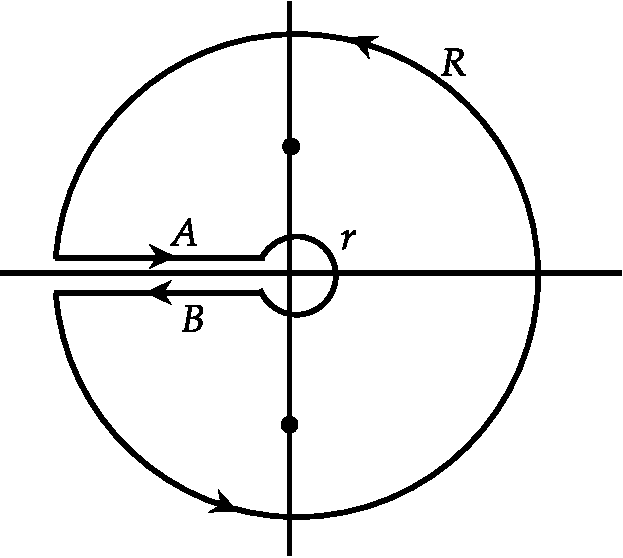
\includegraphics[height=4cm,width=4.6cm]{JEST 01 2012}
	\end{figure}
	\begin{align*}
	\int_{0}^{\infty} \frac{\ln x}{\left(x^{2}+1\right)^{2}} d x&=\int_{0}^{\infty} \frac{\ln z}{\left(z^{2}+1\right)^{2}} d z\\
	\text{Let us consider new function }f(z)&=\left(\frac{\ln z}{z^{2}+1}\right)^{2},\text{ then }I=\int_{0}^{\infty}\left(\frac{\ln z}{z^{2}+1}\right)^{2} d z\\
\text{	Pole at }z&=\pm i\text{ is simple pole of second order.}\\
\text{	Residue at }z&=i\text{ is}\\
&=\frac{d}{d z}(z-i)^{2} \frac{(\ln z)^{2}}{(z-i)^{2}(z+i)^{2}}=\frac{d}{d z} \frac{(\ln z)^{2}}{(z+i)^{2}}\\
&=\frac{(z+i)^{2} 2(\ln z) \cdot \frac{1}{z}-(\ln z)^{2} \cdot 2(z+i)}{(z+i)^{4}}=\frac{(z+i) 2 \ln (z) \frac{1}{z}-(\ln z)^{2} \cdot 2}{(z+i)^{3}}\\
&=\frac{(2 i) 2 \times \frac{1}{i} \ln i-(\ln i)^{2} \cdot 2}{(2 i)^{3}}=\frac{4 \frac{i \pi}{2}-\left(\frac{i \pi}{2}\right)^{2} \times 2}{-8 i}=\frac{2 \pi i+\frac{\pi^{2}}{2}}{-8 i}\\
\left.\Rightarrow \operatorname{Res}\right|_{z=i}&=\frac{-\pi}{4}+\frac{\pi^{2}}{16} i\\
\text{Similarly, at }z&=-i ;\left.\operatorname{Res}\right|_{z=-i}=\frac{-\pi}{4}-\frac{\pi^{2}}{16} i\\
I&=\int_{0}^{\infty}\left(\frac{\ln z}{z^{2}+1}\right)^{2} d z=2 \pi i\left(\frac{-\pi}{4}+\frac{\pi^{2}}{16} i-\frac{\pi}{4}-\frac{\pi^{2}}{16} i\right)=-\pi^{2} i\\
-\pi^{2} i&=\left(\int_{R} \int_{A} \int_{B}\right) f(z) d z=\left(\iint_{A B}\right) f(z) d z ;\qquad \left[\because \int_{A B}\right.\text{ vanish }]\\
\text{Along path }A ;& \quad z=-x+i \varepsilon\text{ and along path }B ; \quad z=-x-i \varepsilon\\
\text{Thus }-\pi^{2} i&=\left(\iint_{A B}\right) f(z) d z=-\int_{-\infty}^{0}\left[\frac{\ln (-x+i \varepsilon)}{(-x+i \varepsilon)^{2}+1}\right] d x-\int_{0}^{\infty}\left[\frac{\ln (-x-i \varepsilon)}{(-x-i \varepsilon)^{2}+1}\right] d x\\
\Rightarrow-\pi^{2} i&=\int_{0}^{\infty}\left[\frac{\ln (-x+i \varepsilon)}{(-x+i \varepsilon)^{2}+1}\right]^{2} d x-\int_{0}^{\infty}\left[\frac{\ln (-x-i \varepsilon)}{(-x-i \varepsilon)^{2}+1}\right]^{2} d x\\
\Rightarrow-\pi^{2} i&=\int_{0}^{\infty}\left[\frac{\ln (x)+i \pi}{1+x^{2}}\right]^{2} d x-\int_{0}^{\infty}\left[\frac{\ln (x)-i \pi}{1+x^{2}}\right]^{2} d x ; \quad \varepsilon \rightarrow 0\\
\Rightarrow-\pi^{2} i&=\int_{0}^{\infty} \frac{(\ln (x)+i \pi)^{2}-(\ln (x)-i \pi)^{2}}{\left(1+x^{2}\right)^{2}} d x\\&=4 \pi i \int_{0}^{\infty} \frac{\ln x}{\left(x^{2}+1\right)^{2}} \Rightarrow \int_{0}^{\infty} \frac{\ln x}{\left(x^{2}+1\right)^{2}}=\frac{-i \pi^{2}}{4 \pi i}=\frac{-\pi}{4}
	\end{align*}
		So the correct answer is \textbf{Option (B)}
\end{answer}
\item Compute $\lim _{z \rightarrow 0} \frac{\operatorname{Re}\left(z^{2}\right)+\operatorname{Im}\left(z^{2}\right)}{z^{2}}$
{\exyear{ JEST 2013}}
 \begin{tasks}(2)
	\task[\textbf{a.}] The limit does not exist
	\task[\textbf{b.}]1
	\task[\textbf{c.}]$-i$
	\task[\textbf{d.}] $-1$
\end{tasks}
\begin{answer}
	\begin{align*}
	\lim _{z \rightarrow 0} \frac{\operatorname{Re}\left(z^{2}\right)+\operatorname{Im}\left(z^{2}\right)}{z^{2}}&=\lim _{z \rightarrow 0} \frac{x^{2}-y^{2}+2 x y}{x^{2}-y^{2}+2 i x y}=\lim _{y=0 \atop x \rightarrow 0} \frac{x^{2}-y^{2}+2 x y}{x^{2}-y^{2}+2 i x y}=1\\
	\lim _{x=0 \atop y \rightarrow 0} \frac{x^{2}-y^{2}+2 x y}{x^{2}-y^{2}+2 i x y}&=1\text{ and }\lim _{y=x \atop x \rightarrow 0} \frac{x^{2}-y^{2}+2 x y}{x^{2}-y^{2}+2 i x y}=-i
	\end{align*}
		So the correct answer is \textbf{Option (A)}
\end{answer}
\item The value of limit
$$
\lim _{z \rightarrow i} \frac{z^{10}+1}{z^{6}+1}
$$
is equal to
{\exyear{ JEST 2014}}
 \begin{tasks}(2)
	\task[\textbf{a.}]1
	\task[\textbf{b.}]0
	\task[\textbf{c.}] $\frac{-10}{3}$
	\task[\textbf{d.}] $\frac{5}{3}$
\end{tasks}
\begin{answer}
	\begin{align*}
	\lim _{z \rightarrow i} \frac{z^{10}+1}{z^{6}+1}=\lim _{z \rightarrow i} \frac{10 z^{9}}{6 z^{5}}=\lim _{z \rightarrow i} \frac{10 z^{4}}{6}=\frac{10}{6}=\frac{5}{3}
	\end{align*}
		So the correct answer is \textbf{Option (D)}
\end{answer}
\item The value of integral
$$
I=\oint \frac{\sin z}{2 z-\pi} d z
$$
with $c$ a circle $|z|=2$, is
{\exyear{ JEST 2014}}
 \begin{tasks}(2)
	\task[\textbf{a.}] 0
	\task[\textbf{b.}]$2 \pi i$
	\task[\textbf{c.}] $\pi i$
	\task[\textbf{d.}]  $-\pi i$
\end{tasks}
\begin{answer}
	\begin{align*}
	I&=\oint_{C} \frac{\sin z}{2 z-\pi},\text{ for pole }2 z-\pi=0 \Rightarrow z=\frac{\pi}{2}\\
\text{	Residue at }z&=\frac{\pi}{2}
	\because|z|=2\text{, so pole will lie within the contour}\\
	I&=\oint_{C} \frac{e^{i z}}{2\left(z-\frac{\pi}{2}\right)}=\sum R \times 2 \pi i\\
	\left.\operatorname{Res}\right|_{z=\frac{\pi}{2}}&=\frac{\left(z-\frac{\pi}{2}\right) e^{i z}}{2\left(z-\frac{\pi}{2}\right)}=\frac{e^{i \pi / 2}}{2}=\frac{i}{2}\text{ (taking imaginary part); Residue }=\frac{1}{2}\\
	\text{Now, }I&=\frac{1}{2} \times 2 \pi i=\pi i
	\end{align*}
		So the correct answer is \textbf{Option (C)}
\end{answer}
\item Given an analytic function $f(z)=\phi(x, y)+i \psi(x, y)$, where $\phi(x, y)=x^{2}+4 x-y^{2}+2 y$
If $C$ is a constant, which of the following relations is true?
{\exyear{ JEST 2015}}
 \begin{tasks}(2)
	\task[\textbf{a.}]$\psi(x, y)=x^{2} y+4 y+C$
	\task[\textbf{b.}]$\psi(x, y)=2 x y-2 x+C$
	\task[\textbf{c.}]$\psi(x, y)=2 x y+4 y-2 x+C$
	\task[\textbf{d.}] $\psi(x, y)=x^{2} y-2 x+C$
\end{tasks}
\begin{answer}
	\begin{align}
	u&=\phi(x, y)=x^{2}+4 x-y^{2}+2 y, v=\psi\notag\\
	\text{From C.R. equation, }\frac{\partial u}{\partial x}&=\frac{\partial v}{\partial y}, \Rightarrow \frac{\partial \phi}{\partial x}=\frac{\partial \psi}{\partial y}, \frac{\partial u}{\partial y}=-\frac{\partial v}{\partial x} \Rightarrow \frac{\partial \phi}{\partial y}=-\frac{\partial \psi}{\partial x}\notag\\
	\text{Now, }\frac{\partial \phi}{\partial x}&=2 x+4=\frac{\partial \psi}{\partial y}\notag\\
	\Rightarrow \psi&=2 x y+4 y+f(x)\label{CN 01}\\
	\text{and }\frac{\partial \phi}{\partial y}&=-2 y+2 \Rightarrow \frac{\partial \psi}{\partial x}=+2 y-2\notag\\
	\psi&=2 x y+2 x+f(y)\label{CN 02}\\
	\text{From (\ref{CN 01}) and (\ref{CN 02}), }&2 x y+4 y+f(x)=2 x y-2 x+f(y)\notag\\
	f(x)&=-2 x, \quad f(y)=4 y \notag\\
	\psi&=2 x y+4 y-2 x+c\notag
	\end{align}
		So the correct answer is \textbf{Option (C)}
\end{answer}
\item Which one is the image of the complex domain $\{z \mid x y \geq 1, x+y>0\}$ under the mapping $f(z)=z^{2}$, if $z=x+i y ?$
{\exyear{ JEST 2017}}
 \begin{tasks}(2)
	\task[\textbf{a.}] $\{z \mid x y \geq 1, x+y>0\}$
	\task[\textbf{b.}]$\{z \mid x \geq 2, x+y>0\}$
	\task[\textbf{c.}]$\{z \mid y \geq 2 \forall x\}$
	\task[\textbf{d.}] $\{z \mid y \geq 1 \forall x\}$
\end{tasks}
\item The integral $I=\int_{1}^{\infty} \frac{\sqrt{x-1}}{(1+x)^{2}} d x$ is
{\exyear{ JEST 2017}}
 \begin{tasks}(2)
	\task[\textbf{a.}]$\frac{\pi}{\sqrt{2}}$
	\task[\textbf{b.}]$\frac{\pi}{2 \sqrt{2}}$
	\task[\textbf{c.}]$\frac{\sqrt{\pi}}{2}$
	\task[\textbf{d.}]$\sqrt{\frac{\pi}{2}}$
\end{tasks}
\begin{answer}
	\begin{align*}
	I&=\int_{1}^{\infty} \frac{\sqrt{x-1}}{(1+x)^{2}} d x\\
\text{	Put,} x&=\left(1+z^{2}\right), d x=2 z d z\\
	\text{Hence, }I&=\int_{0}^{\infty} \frac{2 z^{2} d z}{\left(2+z^{2}\right)^{2}}\\
	\text{Here poles, }\left(2+z^{2}\right)&=0 \Rightarrow(z+i \sqrt{2})(z-i \sqrt{2})=0\\
\text{	Only }&(z=i \sqrt{2})\text{ poles is allowed}\\
\text{Then }R(i \sqrt{2})&=\lim _{z \rightarrow i \sqrt{2}} \frac{1}{\sqrt{2-1}} \frac{d}{d z}\left[\frac{2 z^{2}(z-i \sqrt{2})^{2}}{(z-i \sqrt{2})^{2}(z+i \sqrt{2})^{2}}\right]\\
&=\lim _{z \rightarrow i \sqrt{2}}\left[\frac{(z+i \sqrt{2})^{2} \cdot 4 z-2 z^{2} \cdot 2(z+i \sqrt{2})}{(z+i \sqrt{2})^{4}}\right]\\
&=\frac{(2 i \sqrt{2})^{2} \times 4(i \sqrt{2})-2(i \sqrt{2})^{2} \cdot 2(2 i \sqrt{2})}{(2 i \sqrt{2})^{4}}\\&=-\frac{32 \sqrt{2} i+16 \sqrt{2} i}{64}=-\frac{16 \sqrt{2} i}{64}=-\frac{i}{2 \sqrt{2}}\\
\text{Hence, }\int_{-\infty}^{\infty} \frac{2 z^{2}}{\left(2+z^{2}\right)^{2}} d z&=2 \pi i\left(-\frac{i}{2 \sqrt{2}}\right)=\frac{\pi}{\sqrt{2}}\\
\Rightarrow \int_{0}^{\infty} \frac{2 z^{2}}{\left(2+z^{2}\right)^{2}} d z&=\frac{\pi}{2 \sqrt{2}} \Rightarrow \int_{i}^{\infty} \frac{\sqrt{x-1}}{(1+x)^{2}} d x=\frac{\pi}{2 \sqrt{2}}
	\end{align*}
	So the correct answer is \textbf{Option (B)}
\end{answer}
\item The integral
$$
\int_{-\infty}^{\infty} \frac{\cos x}{x^{2}+1} d x \text { is }
$$
{\exyear{ JEST 2018}}
 \begin{tasks}(2)
	\task[\textbf{a.}]$\frac{\pi}{e}$
	\task[\textbf{b.}] $\pi e^{-2}$
	\task[\textbf{c.}]$\pi$
	\task[\textbf{d.}] zero
\end{tasks}
\begin{answer}
	\begin{align*}
	f(z)&=\frac{e^{i z}}{z^{2}+1}=\frac{e^{i z}}{(z+i)(z-i)}\\
	\int_{-\infty}^{\infty} \frac{\cos x}{x^{2}+1} d x&=\operatorname{Re} 2 \pi i \times \frac{e^{i \cdot i}}{z i}=\frac{\pi}{e}
	\end{align*}
		So the correct answer is \textbf{Option (A)}
\end{answer}
\item Consider the function $f(x, y)=|x|-i|y| .$ In which domain of the complex plane is this function analytic?
{\exyear{ JEST 2019}}
 \begin{tasks}(2)
	\task[\textbf{a.}]First and second quadrants
	\task[\textbf{b.}]Second and third quadrants
	\task[\textbf{c.}]Second and fourth quadrants
	\task[\textbf{d.}]  Nowhere
\end{tasks}
\begin{answer}
	\begin{align*}
	 f(x, y)&=|x|-i|y|\\
	f(x, y)&=x-i y=\bar{z}\\
	f(x, y)&=-x-i y=-z\\
	f(x, y)&=-x+i y=-\bar{z}\\
	f(x, y)&=x+i y=z
	\intertext{We know $\bar{z}$ is not analytic and $z$ and $-z$ are analytic. }
	\end{align*}
	So the correct answer is \textbf{Option (C)}
\end{answer}
\end{enumerate}
 \colorlet{ocre1}{ocre!70!}
\colorlet{ocrel}{ocre!30!}
\setlength\arrayrulewidth{1pt}
\begin{table}[H]
	\centering
	\arrayrulecolor{ocre}
	\begin{tabular}{|p{1.5cm}|p{1.7cm}||p{1.5cm}|p{1.5cm}|}
		\hline
		\multicolumn{4}{|c|}{\textbf{Answer key}}\\\hline\hline
		\rowcolor{ocrel}Q.No.&Answer&Q.No.&Answer\\\hline
		1&\textbf{D} &2&\textbf{C}\\\hline 
		3&\textbf{3(NAT)} &4&\textbf{C} \\\hline
		5&\textbf{A} &6&\textbf{C} \\\hline
		7&\textbf{C}&8&\textbf{A}\\\hline
		9&\textbf{$\pi$(NAT)}&10&\textbf{3(NAT)}\\\hline
		11&\textbf{81.64(NAT)} &12&\textbf{C}\\\hline
		13&\textbf{A}& 14&\textbf{B}\\\hline
		15&\textbf{A}&16 &\textbf{D}\\\hline
		17&\textbf{C}&18&\textbf{C}\\\hline
		19&\textbf{-} &20&\textbf{B}\\\hline
		21&\textbf{A}&22&\textbf{C}\\\hline
	\end{tabular}
\end{table}
%\chapter{Complex Numbers}
A simple algebraic equation like $x^{2}=-1$ may not have a real solution. Introducing complex numbers validates the existence of 'root' for every polynomial with a positive degree . Which then proves the fundamental theorem of algebra. The idea of complex numbers are widely used in Physics and Mathematics.
\begin{definition}
	A number of the form {${x+i y}$} , where $x$ and $y$ are real numbers and $i=\sqrt{(-1)},$ is called a complex number.
\end{definition}
	\textbf{\large Real Part\ \hspace{1.08cm}:} $x$ is called the real part of the complex number,  $x+i y$ and is written as,\ ${{R(x+i y)}}$.\\\\ 
	\textbf{\large Imaginary Part\ :} $y$ is called the imaginary part of the complex number and is written as,\ ${I(x+i y)}$.
	\section{Representation of a Complex number}
The point whose cartesian coordinates are $(x, y)$ uniquely
represents the complex number, {${z=x+i y}$} on the complex plane $z$. The diagram in which this representation is carried out is called the Argand's diagram. It's shown in the figure \ref{Argand Diagram}.  Since $x$ is the real part of $z$ we call the $x$ -axis the real axis. Likewise, the $y$ -axis is the imaginary axis.

		\begin{figure}[H]
				\begin{center}
			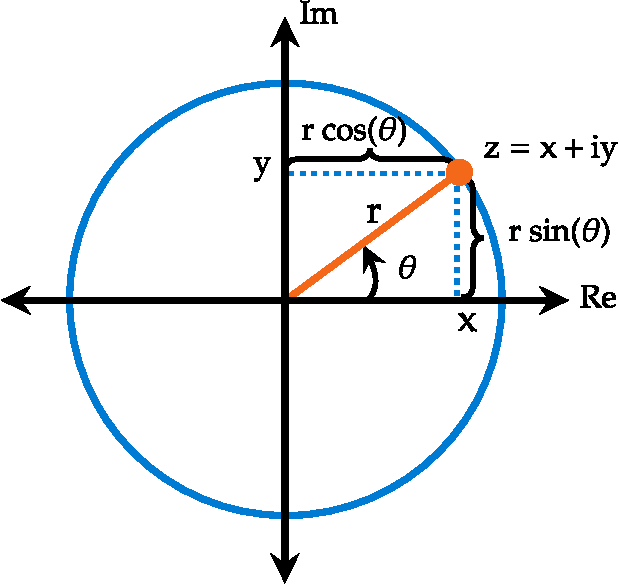
\includegraphics[width=0.30\textwidth]{cn1}
				\end{center}
			\caption{Argand Diagram}
			\label{Argand Diagram}
	    \end{figure}
    In terms of the polar coordinates  , we have
    \begin{align}
    x&=r \cos \theta, \quad y=r \sin \theta\\
    z&=x+\text { iy }=re^{i\theta} \notag \\&=r(\cos \theta+i \sin \theta)
    \label{Euler's equation}
    \end{align}
    Then, the  equation \ref{Euler's equation} is known as, Euler's formula
    \begin{figure}[H]
    	\begin{minipage}{0.40\textwidth}
    		\begin{center}
    		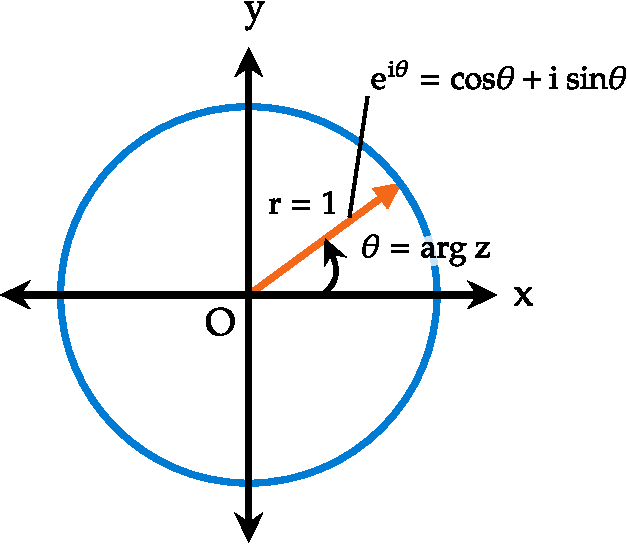
\includegraphics[width=0.70\textwidth]{cn2}
    	\end{center}
    	\end{minipage}\hfil
    	\begin{minipage}{0.40\textwidth}
    	\begin{center}
    		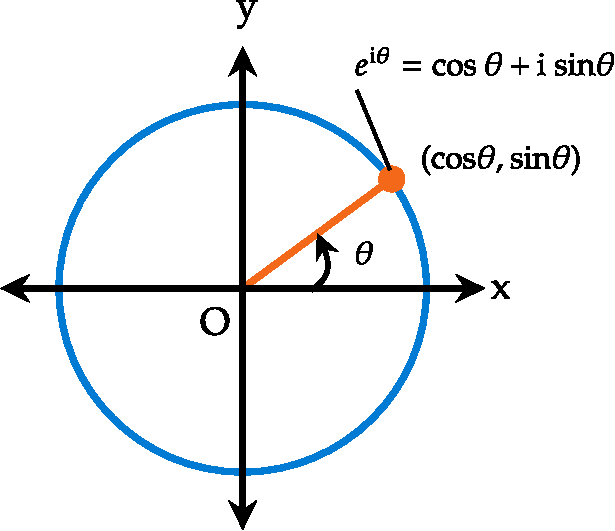
\includegraphics[width=0.70\textwidth]{cn3}
    	\end{center}
    \end{minipage}
    
    \caption{Polar representation}
    \end{figure}
   \subsection{Absolute Value}
    We define the absolute value of a complex number $x+i y$ to be the length ${r}$ of the vector from the origin to $P(x, y)$. 
    $$
    r=|x+i y|=\sqrt{x^{2}+y^{2}}
    $$
    \\\textbf{Properties:}
    \begin{itemize}
    	\item $\left|z_{1}+z_{2}\right| \leq\left|z_{1}\right|+\left|z_{2}\right|$
    	\item $\left|z_{1}-z_{2}\right| \geq\left|z_{1}\right|-\left|z_{2}\right|$
    	\item $\left|z_{1} z_{2}\right|=\left|z_{1}\right|\left|z_{2}\right|$
    	\item $\left|\frac{z_{1}}{z_{2}}\right|=\frac{\left|z_{1}\right|}{\left|z_{2}\right|}$
    \end{itemize}
    \subsection{Argument of $\mathbf{z}$ }
    The polar angle $\theta$ is called the {argument} of $z$ and it is written as, $${\theta=\arg z }$$ Any integer multiple of $2 \pi$ may be added to $\theta$ to produce another appropriate  angle.\\From the figure \ref{Argand Diagram},
    $${\theta=\arg z }=\tan ^{-1}\left(\frac{y}{x}\right)$$
    \\\textbf{Properties:}
    \begin{itemize}
    	\item $\operatorname{Arg}\left(z_{1}  z_{2} \cdot z_{3} \ldots \ldots z_{n}\right)=\operatorname{Arg} \left(z_{1}\right)+\operatorname{Arg}  \left(z_{2}\right)+\operatorname{Arg}  \left(z_{3}\right)+\ldots \ldots . .+\operatorname{Arg}\left(z_{n}\right)$
    	\item $\operatorname{Arg}\left(\frac{z_{1}}{z_{2}}\right)=\operatorname{Arg}\left(z_{1}\right)-\operatorname{Arg}\left(z_{2}\right)$
    \end{itemize}
\begin{exercise}
	Find the modulus and principal argument of the complex number
	$\frac{1+2 i}{1-(1-i)^{2}}$
\end{exercise}
\begin{answer}
	\begin{align*}
	\frac{1+2 i}{1-(1-i)^{2}}&=\frac{1+2 i}{1-(1-1-2 i)}=\frac{1+2 i}{1+2 i}\\&=1=1+0 i \\
	\therefore \quad\left|\frac{1+2 i}{1-(1-i)^{2}}\right|&=|1+0 i|=\sqrt{1^{2}}=1\\
	\text{Principal argument of}\ \frac{1+2 i}{1-(1-i)^{2}}&= \text{Principal argument of} \quad \left( 1+0 i\right) \\
	\tan ^{-1} \frac{0}{1}&=\tan ^{-1} 0\\&=0^{\circ}
	\end{align*}
\end{answer}

     \subsection{Conjugate of a Complex number}
	The conjugate of a complex number $z$ is represented by, $${\bar{z}=x-i y}$$
	\begin{note}\newline 
	$ \left. \right. $ \hspace{1.5cm}	$\begin{aligned}
		\frac{z + \bar{z}}{2}&=Re\left\lbrace z\right\rbrace \\
		\frac{z - \bar{z}}{2i}&=Im\left\lbrace z\right\rbrace\\
		z \cdot \bar{z}&=|z|^{2}
		\end{aligned}$
	\end{note}

\section{Algebra of Complex numbers}
For two Complex numbers, $a+i b$ and $c+i d $
\subsubsection{Equality:}
	\begin{align*}
	a+i b&=c+i d \quad
	\end{align*}
	Two complex numbers $(a, b)$
 and $(c, d)$ are equal if and only $a=c$ and $b=d$.
 \subsubsection{Addition:} 
 \begin{align*}
 (a+i b)+(c+i d) \quad&=(a+c)+i(b+d) \quad
 \end{align*}
 \subsubsection{Multiplication:} \begin{align*}
 (a+i b)(c+i d) &=(a c-b d)+i(a d+b c) \\
 c(a+i b)&=a c+i(b c)
 \end{align*}
 \textbf{Polar form:} 
 \begin{align*} 
 \text{Let,} \quad z_{1}&=r_{1}\left(\cos \theta_{1}+i \sin \theta_{1}\right) \quad \text{and}\quad z_{2}=r_{2}\left(\cos \theta_{2}+i \sin \theta_{2}\right)\\
 z_{1} . z_{2} &=r_{1} r_{2}\left(\cos \theta_{1}+i \sin \theta_{1}\right)\left(\cos \theta_{2}+i \sin \theta_{2}\right) \\ &=r_{1} r_{2}\left[\cos \theta_{1} \cos \theta_{2}-\sin \theta_{1} \sin \theta_{2}+i\left(\sin \theta_{1} \cos \theta_{2}+\cos \theta_{1} \sin \theta_{2}\right)\right] \\ &=r_{1} r_{1}\left[\cos \left(\theta_{1}+\theta_{2}\right)+i \sin \left(\theta_{1}+\theta_{2}\right)\right], \end{align*}
 
 \subsubsection{Division:}\begin{align*}
 \frac{c+i d}{a+i b}&=\frac{(c+i d)(a-i b)}{(a+i b)(a-i b)}\\&=\frac{(a c+b d)+i(a d-b c)}{a^{2}+b^{2}}\\
 \text{Where,}\quad x&=\frac{a c+b d}{a^{2}+b^{2}},\quad \text{and} \quad y=\frac{a d-b c}{a^{2}+b^{2}}
 \end{align*}
 \textbf{Polar form:}\\ Let $z_{1}=r_{1}\left(\cos \theta_{1}+i \sin \theta_{1}\right)$ and $z_{2}=r_{2}\left(\cos \theta_{2}+i \sin \theta_{2}\right)$\\\\\\
 $\begin{aligned} \frac{z_{1}}{z_{2}} &=\frac{r_{1}\left(\cos \theta_{1}+i \sin \theta_{1}\right)}{r_{2}\left(\cos \theta_{2}+i \sin \theta_{2}\right)}\\\\&=\frac{r_{1}\left(\cos \theta_{1}+i \sin \theta_{1}\right)\left(\cos \theta_{2}-i \sin \theta_{2}\right)}{r_{2}\left(\cos \theta_{2}+i \sin \theta_{2}\right)\left(\cos \theta_{2}-i \sin \theta_{2}\right)} \\\\ &=\frac{r_{1}\left[\left(\cos \theta_{1} \cos \theta_{2}+\sin \theta_{1} \sin \theta_{2}\right)+i\left(\sin \theta_{1} \cos \theta_{2}-\sin \theta_{2} \cos \theta_{1}\right)\right]}{r_{2}\left(\cos ^{2} \theta_{2}+\sin ^{2} \theta_{2}\right)} \\ &=\frac{r_{1}}{r_{2}}\left[\cos \left(\theta_{1}-\theta_{2}\right)+i \sin \left(\theta_{1}-\theta_{2}\right)\right] \end{aligned}$
\begin{exercise}
	Find
	\begin{enumerate}
		\item $(2+3 i)+(6-2 i)$
		\item $(2+3 i)-(6-2 i) $
		\item $(2+3 i)(6-2 i)$
		\item $\frac{2+3 i}{6-2 i}$
	\end{enumerate}
\end{exercise}
\begin{answer}\hspace{0.5cm}
		\begin{enumerate}
		\item $(2+3 i)+(6-2 i)=(2+6)+(3-2) i=8+i $
		
		\item $(2-6)+(3-(-2)) i=-4+5 i $
		\item
		\begin{align*}
		(2+3 i)(6-2 i)&=(2)(6)+(2)(-2 i)+(3 i)(6)+(3 i)(-2 i)\\
		&=12-4 i+18 i-6 i^{2}\\&=12+14 i+6=18+14 i
		\end{align*}
		\item 
		\begin{align*}
		\frac{2+3 i}{6-2 i}&=\frac{2+3 i}{6-2 i} \frac{6+2 i}{6+2 i}\\
		&=\frac{12+4 i+18 i+6 i^{2}}{36+12 i-12 i-4 i^{2}}\\
		&=\frac{6+22 i}{40}\\&=\frac{3}{20}+\frac{11}{20} i
		\end{align*}
	\end{enumerate}
\end{answer}
\begin{exercise}
	Express $\frac{(6+i) \cdot(2-i)}{(4+3 i) \cdot(1-2 i)}$ in the form of $a+i b$
\end{exercise}
\begin{answer}
	\begin{align*} \frac{(6+i) \cdot(2-i)}{(4+3 i) \cdot(1-2 i)} &=\frac{12+1+i(2-6)}{4+6+i(3-8)}=\frac{13-4 i}{10-5 i} \\ &=\frac{(13-4 i)(10+5 i)}{(10-5 i)(10+5 i)}=\frac{150+25 i}{100+25}\\&=\frac{6+i}{5}\\&=\frac{6}{5}+\frac{1}{5} i \end{align*}
\end{answer}


\section{Important Identities}
\subsection{Circular functions of Complex numbers}

\begin{align*}
	\bullet\quad\sin \theta=\frac{e^{i \theta}-e^{-i \theta}}{2 i}\quad\bullet&\quad\cos \theta=\frac{e^{i \theta}+e^{-i \theta}}{2}\\\\
\bullet\quad\sin z=\frac{e^{i z}-e^{-i z}}{2 i}\quad\bullet&\quad\cos z=\frac{e^{i z}+e^{-i z}}{2}
\end{align*}

\subsection{Hyperbolic functions of Complex numbers}
\begin{alignat*}{2}
&\bullet\quad \sinh x=\frac{e^{x}-e^{-x}}{2}\quad&&\bullet\quad \cosh x=\frac{e^{x}+e^{-x}}{2}\\
&\bullet\quad\tanh x=\frac{e^{x}-e^{-x}}{e^{x}+e^{-x}}\quad&&\bullet \quad {\coth} x=\frac{e^{x}+e^{-x}}{e^{x}-e^{-x}}
\\
&\bullet\quad{\operatorname{sech}} x=\frac{2}{e^{x}+e^{-x}} \quad&&\bullet \quad {\operatorname{cosech}} x=\frac{2}{e^{x}-e^{-x}}\\
&\bullet\quad\cosh x+\sinh x=\frac{e^{x}+e^{-x}}{2}+\frac{e^{x}-e^{-x}}{2}=e^{x} \quad&& \quad
\end{alignat*}
\begin{note}
\textbf{\textbf{Relation between Circular and Hyperbolic functions:}}\\\\
$\begin{array}{ll}\bullet\quad\sin i x=i \sinh x & \bullet\quad \sinh i x=i \sin x \\ \bullet\quad\cos i x=\cosh x & \bullet\quad \cosh i x=\cos x \\ \bullet\quad\tan i x=i \tanh x& \bullet\quad \tanh i x=i \tan x\end{array}$

\end{note}

\begin{theorem}
	\textbf{De Moivre's Theorem:}
	\begin{enumerate}
		\item For any integer $n,$ $(\cos \theta+i \sin \theta)^{n}=\cos n \theta+i \sin n \theta$
		\item 	If $n$ is a fraction, then $(\cos n \theta+i \sin n \theta)$ is one of the values .
	\end{enumerate}
\end{theorem}
\begin{exercise}
  Express $\frac{(\cos \theta+i \sin \theta)^{8}}{(\sin \theta+i \cos \theta)^{4}}$ in the form $(x+i y)$
\end{exercise}
\begin{answer}
	$$
	\begin{aligned}
	\frac{(\cos \theta+i \sin \theta)^{8}}{(\sin \theta+i \cos \theta)^{4}}=&\frac{(\cos \theta+i \sin \theta)^{8}}{(i)^{4}\left(\cos \theta+\frac{1}{i} \sin \theta\right)^{4}} \\
	=& \frac{(\cos \theta+i \sin \theta)^{8}}{(\cos \theta-i \sin \theta)^{4}}=\frac{(\cos \theta+i \sin \theta)^{8}}{[\cos (-\theta)+i \sin (-\theta)]^{4}} \\
	=& \frac{(\cos \theta+i \sin \theta)^{8}}{\left[(\cos \theta+i \sin \theta)^{-1}\right]^{4}}=\frac{(\cos \theta+i \sin \theta)^{8}}{(\cos \theta+i \sin \theta)^{-4}}=(\cos \theta+i \sin \theta)^{12} \\
	=& \cos 12 \theta+i \sin 12 \theta
	\end{aligned}
	$$
\end{answer}
\begin{note}
	Series expansion of different functions
	
	\begin{align*}
	e^{x}&=1+x+\frac{x^{2}}{2 !}+\frac{x^{3}}{3 !}+\frac{x^{4}}{4 !}+\ldots \\
	\sin x&=x-\frac{x^{3}}{3 !}+\frac{x^{5}}{5 !}-\frac{x^{7}}{7 !}+\ldots \\
	\cos x&=1-\frac{x^{2}}{2 !}+\frac{x^{4}}{4 !}-\frac{x^{6}}{6 !}+\ldots \\
	\tan x&=x+\frac{x^{3}}{3}+\frac{2 x^{5}}{15}+\frac{17 x^{7}}{315}+\frac{62 x^{9}}{2835} +\cdots\\
	\ln (1+x)&=x-\frac{x^{2}}{2}+\frac{x^{3}}{3}-\frac{x^{4}}{4}+\ldots \\
    \tan ^{-1}(x)&=x-\frac{x^{3}}{3}+\frac{x^{5}}{5}-\frac{x^{7}}{7}+\ldots
	\end{align*}
	
\end{note}
\newpage
\begin{abox}
	Practise Set-1
	\end{abox}
\begin{enumerate}[label=\color{ocre}\textbf{\arabic*.}]
	\item The value of the integral $\int_{C} d z z^{2} e^{z}$, where $C$ is an open contour in the complex $z$-plane as shown in the figure below, is:
	{\exyear{NET/JRF(JUNE-2011)}}
	\begin{figure}[H]
		\centering
		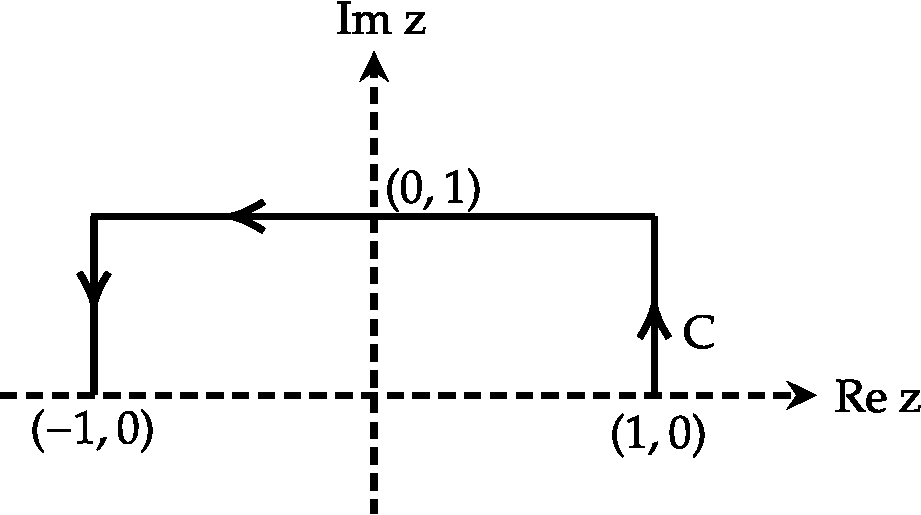
\includegraphics[height=5cm,width=9cm]{diagram-20211005-crop}
	\end{figure}
	\begin{tasks}(4)
		\task[\textbf{A.}] $\frac{5}{e}+e$
		\task[\textbf{B.}] $e-\frac{5}{e}$
		\task[\textbf{C.}] $\frac{5}{e}-e$
		\task[\textbf{D.}] $-\frac{5}{e}-e$
	\end{tasks}
	\item Which of the following is an analytic function of the complex variable $z=x+i y$ in the domain $|z|<2 ?$
	{\exyear{NET/JRF(JUNE-2011)}}
	\begin{tasks}(2)
		\task[\textbf{A.}] $(3+x-i y)^{7}$
		\task[\textbf{B.}] $(1+x+i y)^{4}(7-x-i y)^{3}$
		\task[\textbf{C.}] $(1-x-i y)^{4}(7-x+i y)^{3}$
		\task[\textbf{D.}] $(x+i y-1)^{1 / 2}$
	\end{tasks}
	\item The first few terms in the Laurent series for $\frac{1}{(z-1)(z-2)}$ in the region $1 \leq|z| \leq 2$ and around $z=1$ is
	{\exyear{NET/JRF(JUNE-2012)}}
	\begin{tasks}(1)
		\task[\textbf{A.}] $\frac{1}{2}\left[1+z+z^{2}+\ldots\right]\left[1+\frac{z}{2}+\frac{z^{2}}{4}+\frac{z^{3}}{8}+\ldots .\right]$
		\task[\textbf{B.}] $\frac{1}{1-z}-z-(1-z)^{2}+(1-z)^{3}+\ldots .$
		\task[\textbf{C.}] $\frac{1}{\mathrm{z}^{2}}\left[1+\frac{1}{\mathrm{z}}+\frac{1}{\mathrm{z}^{2}}+\ldots .\right]\left[1+\frac{2}{\mathrm{z}}+\frac{4}{\mathrm{z}^{2}}+\ldots . .\right]$
		\task[\textbf{D.}]  $2(z-1)+5(z-1)^{2}+7(z-1)^{3}+\ldots$
	\end{tasks}
	\item Let $u(x, y)=x+\frac{1}{2}\left(x^{2}-y^{2}\right)$ be the real part of analytic function $f(z)$ of the complex variable $z=x+i y$. The imaginary part of $f(z)$ is
	{\exyear{NET/JRF(JUNE-2012)}}
	\begin{tasks}(4)
		\task[\textbf{A.}] $y+x y$
		\task[\textbf{B.}] $x y$
		\task[\textbf{C.}] $y$
		\task[\textbf{D.}] $y^{2}-x^{2}$
	\end{tasks}
	\item The value of the integral $\int_{C} \frac{z^{3} d z}{\left(z^{2}-5 z+6\right)}$, where $C$ is a closed contour defined by the equation $2|z|-5=0$, traversed in the anti-clockwise direction, is
	{\exyear{NET/JRF(DEC-2012)}}
	\begin{tasks}(4)
		\task[\textbf{A.}] $-16 \pi i$
		\task[\textbf{B.}] $16 \pi \mathrm{i}$
		\task[\textbf{C.}] $8 \pi i$
		\task[\textbf{D.}] $2 \pi i$
	\end{tasks}
	\item  With $z=x+i y$, which of the following functions $f(x, y)$ is NOT a (complex) analytic function of $z$ ?
	{\exyear{NET/JRF(JUNE-2013)}}
	\begin{tasks}(1)
		\task[\textbf{A.}] $f(x, y)=(x+i y-8)^{3}\left(4+x^{2}-y^{2}+2 i x y\right)^{7}$
		\task[\textbf{B.}] $f(x, y)=(x+i y)^{7}(1-x-i y)^{3}$
		\task[\textbf{C.}] $f(x, y)=\left(x^{2}-y^{2}+2 i x y-3\right)^{5}$
		\task[\textbf{D.}] $f(x, y)=(1-x+i y)^{4}(2+x+i y)^{6}$
	\end{tasks}
	\item  Which of the following functions cannot be the real part of a complex analytic function of $z=x+i y ?$
	{\exyear{NET/JRF(DEC-2013)}}
	\begin{tasks}(4)
		\task[\textbf{A.}] $x^{2} y$
		\task[\textbf{B.}]  $x^{2}-y^{2}$
		\task[\textbf{C.}] $x^{3}-3 x y^{2}$
		\task[\textbf{D.}] $3 x^{2} y-y-y^{3}$
	\end{tasks}
	\item  Given that the integral $\int_{0}^{\infty} \frac{d x}{y^{2}+x^{2}}=\frac{\pi}{2 y}$, the value of $\int_{0}^{\infty} \frac{d x}{\left(y^{2}+x^{2}\right)^{2}}$ is
	{\exyear{NET/JRF(DEC-2013)}}
	\begin{tasks}(4)
		\task[\textbf{A.}] $\frac{\pi}{y^{3}}$
		\task[\textbf{B.}] $\frac{\pi}{4 y^{3}}$
		\task[\textbf{C.}]  $\frac{\pi}{8 y^{3}}$
		\task[\textbf{D.}] $\frac{\pi}{2 y^{3}}$
	\end{tasks}
	\item If $C$ is the contour defined by $|z|=\frac{1}{2}$, the value of the integral
	$$
	\oint_{C} \frac{d z}{\sin ^{2} z}
	$$
	is
	{\exyear{NET/JRF(JUNE-2014)}}
	\begin{tasks}(4)
		\task[\textbf{A.}] $\infty$
		\task[\textbf{B.}] $2 \pi i$
		\task[\textbf{C.}] 0
		\task[\textbf{D.}] $\pi i$
	\end{tasks}
	\item The principal value of the integral $\int_{-\infty}^{\infty} \frac{\sin (2 x)}{x^{3}} d x$ is
	{\exyear{NET/JRF(DEC-2014)}}
	\begin{tasks}(4)
		\task[\textbf{A.}] $-2 \pi$
		\task[\textbf{B.}]  $-\pi$
		\task[\textbf{C.}] $\pi$
		\task[\textbf{D.}]  $2 \pi$
	\end{tasks}
	\item The Laurent series expansion of the function $f(z)=e^{2}+e^{1 / 2}$ about $z=0$ is given by
	{\exyear{NET/JRF(DEC-2014)}}
	\begin{tasks}(2)
		\task[\textbf{A.}] $\sum_{n=-\infty}^{\infty} \frac{z^{n}}{n !}$ for all $|z|<\infty$
		\task[\textbf{B.}] $\sum_{n=0}^{\infty}\left(z^{n}+\frac{1}{z^{n}}\right) \frac{1}{n !}$ only if $0<|z|<1$
		\task[\textbf{C.}] $\sum_{n=0}^{\infty}\left(z^{n}+\frac{1}{z^{n}}\right) \frac{1}{n !}$ for all $0<|z|<\infty$
		\task[\textbf{D.}]  $\sum_{n=-\infty}^{\infty} \frac{z^{n}}{n !}$ only if $|z|<1$
	\end{tasks}
	\item Consider the function $f(z)=\frac{1}{z} \ln (1-z)$ of a complex variable $z=r e^{i \theta}(r \geq 0, \quad-\infty<\theta<\infty)$. The singularities of $f(z)$ are as follows:
	{\exyear{NET/JRF(DEC-2014)}}
	\begin{tasks}(1)
		\task[\textbf{A.}]  Branch points at $z=1$ and $z=\infty$; and a pole at $z=0$ only for $0 \leq \theta<2 \pi$
		\task[\textbf{B.}] Branch points at $z=1$ and $z=\infty$; and a pole at $z=0$ for all $\theta$ other than $0 \leq \theta<2 \pi$
		\task[\textbf{C.}] Branch points at $z=1$ and $z=\infty$; and a pole at $z=0$ for all $\theta$
		\task[\textbf{D.}] Branch points at $z=0, z=1$ and $z=\infty$.
	\end{tasks}
	\item  The value of integral $\int_{-\infty}^{\infty} \frac{d x}{1+x^{4}}$
	{\exyear{NET/JRF(JUNE-2015)}}
	\begin{tasks}(4)
		\task[\textbf{A.}] $\frac{\pi}{\sqrt{2}}$
		\task[\textbf{B.}] $\frac{\pi}{2}$
		\task[\textbf{C.}] $\sqrt{2} \pi$
		\task[\textbf{D.}] $2 \pi$
	\end{tasks}
	\item  The function $\frac{Z}{\sin \pi z^{2}}$ of a complex variable $z$ has
	{\exyear{NET/JRF(DEC-2015)}}
	\begin{tasks}(1)
		\task[\textbf{A.}] A simple pole at 0 and poles of order 2 at $\pm \sqrt{n}$ for $n=1,2,3 \ldots$
		\task[\textbf{B.}] A simple pole at 0 and poles of order 2 at $\pm \sqrt{n}$ and $\pm i \sqrt{n}$ for $n=1,2,3 \ldots$
		\task[\textbf{C.}] Poles of order 2 at $\pm \sqrt{n}, n=0,1,2,3 \ldots$
		\task[\textbf{D.}] Poles of order 2 at $\pm n, n=0,1,2,3 \ldots$
	\end{tasks}
	\item The value of the contour integral $\frac{1}{2 \pi i} \oint_{C} \frac{e^{4 z}-1}{\cosh (z)-2 \sinh (z)} d z$ around the unit circle $C$ traversed in the anti-clockwise direction, is
	{\exyear{NET/JRF(JUNE-2016)}}
	\begin{tasks}(4)
		\task[\textbf{A.}] 0
		\task[\textbf{B.}] 2
		\task[\textbf{C.}] $\frac{-8}{\sqrt{3}}$
		\task[\textbf{D.}] $-\tanh \left(\frac{1}{2}\right)$
	\end{tasks}
	\item  Let $u(x, y)=e^{a x} \cos (b y)$ be the real part of a function $f(z)=u(x, y)+i v(x, y)$ of the complex variable $z=x+i y$, where $a, b$ are real constants and $a \neq 0 .$ The function $f(z)$ is complex analytic everywhere in the complex plane if and only if
	{\exyear{NET/JRF(JUNE-2017)}}
	\begin{tasks}(4)
		\task[\textbf{A.}] $b=0$
		\task[\textbf{B.}] $b=\pm a$
		\task[\textbf{C.}] $b=\pm 2 \pi a$
		\task[\textbf{D.}]  $b=a \pm 2 \pi$
	\end{tasks}
	\item  The integral $\oint_{\Gamma} \frac{z e^{i \pi z / 2}}{z^{2}-1} d z$ along the closed contour $\Gamma$ shown in the figure is
	{\exyear{NET/JRF(JUNE-2017)}}
	\begin{figure}[H]
		\centering
		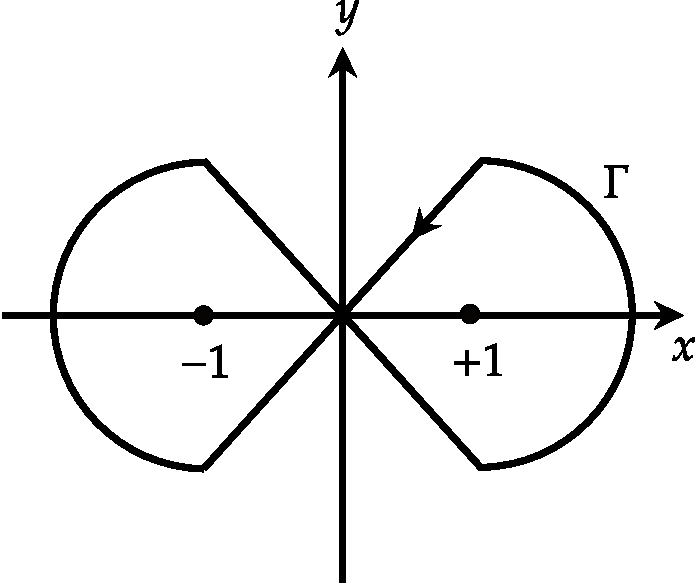
\includegraphics[height=4cm,width=5cm]{diagram-20211005(19)-crop}
	\end{figure}
	\begin{tasks}(4)
		\task[\textbf{A.}] 0
		\task[\textbf{B.}] $2 \pi$
		\task[\textbf{C.}] $-2 \pi$
		\task[\textbf{D.}] $4 \pi i$
	\end{tasks}
	\item What is the value of $a$ for which $f(x, y)=2 x+3\left(x^{2}-y^{2}\right)+2 i(3 x y+a y)$ is an analytic function of complex variable $z=x+i y$
	{\exyear{NET/JRF(JUNE-2018)}}
	\begin{tasks}(4)
		\task[\textbf{A.}] 1
		\task[\textbf{B.}] 0
		\task[\textbf{C.}] 3
		\task[\textbf{D.}] 2
	\end{tasks}
\item  The value of the integral $\oint_{C} \frac{d z}{z} \frac{\tanh 2 z}{\sin \pi z}$, where $C$ is a circle of radius $\frac{\pi}{2}$, traversed counter-clockwise, with centre at $z=0$, is
{\exyear{NET/JRF(DEC-2018)}}
\begin{tasks}(4)
	\task[\textbf{A.}] 4
	\task[\textbf{B.}] $4 i$
	\task[\textbf{C.}] $2 i$
	\task[\textbf{D.}] 0
\end{tasks}
	\item The integral $I=\int_{C} e^{z} d z$ is evaluated from the point $(-1,0)$ to $(1,0)$ along the contour $C$, which is an arc of the parabola $y=x^{2}-1$, as shown in the figure. The value of $I$ is
	{\exyear{NET/JRF(DEC-2018)}}
	\begin{figure}[H]
		\centering
		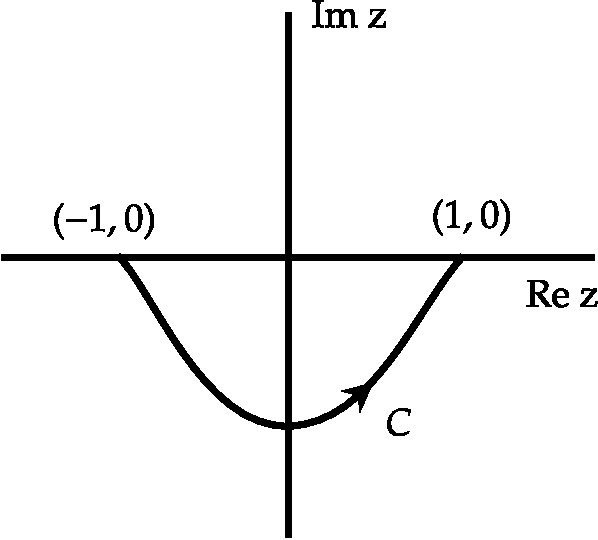
\includegraphics[height=4.5cm,width=5cm]{diagram-20211005(3)-crop}
	\end{figure}
	\begin{tasks}(4)
		\task[\textbf{A.}]  0
		\task[\textbf{B.}] $2 \sinh 1$
		\task[\textbf{C.}]  $e^{2 i} \sinh 1$
		\task[\textbf{D.}] $e+e^{-1}$
	\end{tasks}
	\item The contour $C$ of the following integral
	$$
	\oint_{C} d z \frac{\sqrt{(z-1)(z-3)}}{\left(z^{2}-25\right)^{3}}
	$$
	in the complex $z$ plane is shown in the figure below.\\
	\begin{figure}[H]
		\centering
		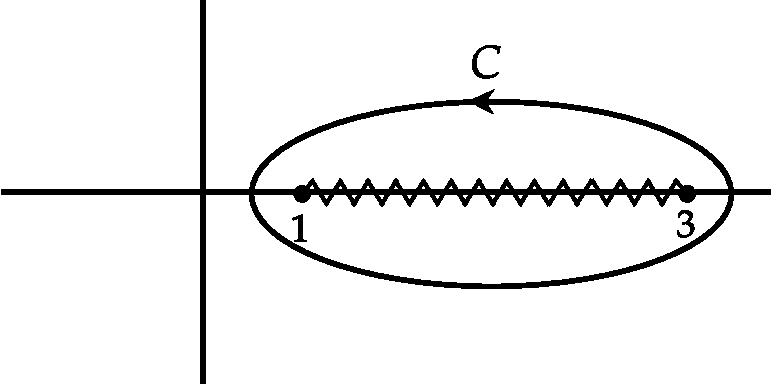
\includegraphics[height=3.5cm,width=6cm]{diagram-20211005(8)-crop}
	\end{figure}
	This integral is equivalent to an integral along the contours
	{\exyear{NET/JRF(DEC-2018)}}
	\begin{tasks}(2)
		\task[\textbf{A.}] \begin{figure}[H]
			\centering
			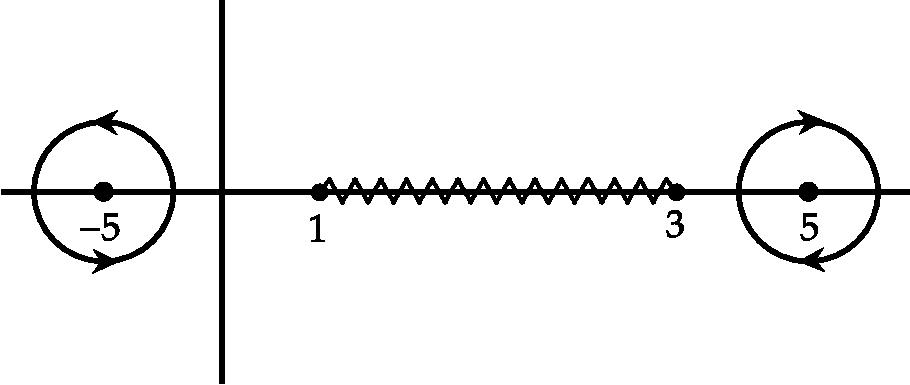
\includegraphics[height=3cm,width=6.5cm]{diagram-20211005(4)-crop}
		\end{figure}
		\task[\textbf{B.}] \begin{figure}[H]
			\centering
			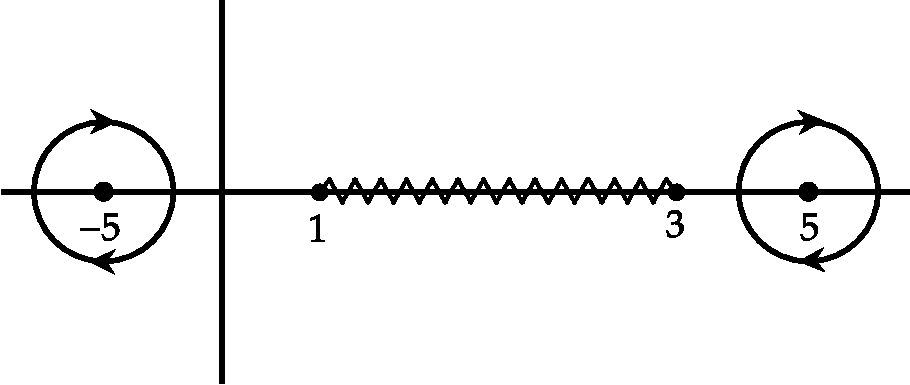
\includegraphics[height=3cm,width=6.5cm]{diagram-20211005(5)-crop}
		\end{figure}
		\task[\textbf{C.}] \begin{figure}[H]
			\centering
			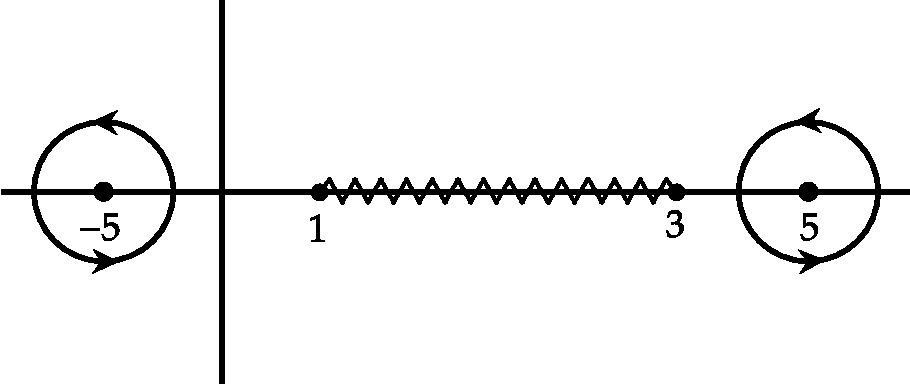
\includegraphics[height=3cm,width=6.5cm]{diagram-20211005(6)-crop}
		\end{figure}
		\task[\textbf{D.}] \begin{figure}[H]
			\centering
			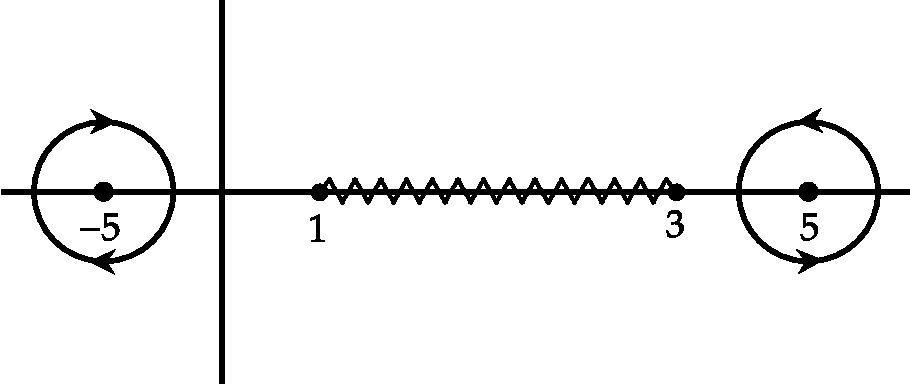
\includegraphics[height=3cm,width=6.5cm]{diagram-20211005(7)-crop}
		\end{figure}
	\end{tasks}
	\item  Let $C$ be the circle of radius $\frac{\pi}{4}$ centered at $z=\frac{1}{4}$ in the complex $z$-plane that is traversed counter-clockwise. The value of the contour integral $\oint_{C} \frac{z^{2}}{\sin ^{2} 4 z} d z$ is
	{\exyear{NET/JRF(DEC-2019)}}
	\begin{tasks}(4)
		\task[\textbf{A.}] 0
		\task[\textbf{B.}] $\frac{i \pi^{2}}{4}$
		\task[\textbf{C.}] $\frac{i \pi^{2}}{16}$
		\task[\textbf{D.}] $\frac{i \pi}{4}$
	\end{tasks}
	\item  A function of a complex variable $z$ is defined by the integral $f(z)=\oint_{\Gamma} \frac{w^{2}-2}{w-z} d w$, where $\Gamma$ is a circular contour of radius 3 , centred at origin, running counter-clockwise in the $w$ - plane. The value of the function at $z=(2-i)$ is
	{\exyear{NET/JRF(JUNE-2020)}}
	\begin{tasks}(4)
		\task[\textbf{A.}] 0
		\task[\textbf{B.}] $1-4 i$
		\task[\textbf{C.}]  $8 \pi+2 \pi \mathrm{i}$
		\task[\textbf{D.}] $-\frac{2}{\pi}-\frac{i}{2 \pi}$
	\end{tasks}
\end{enumerate}
 \colorlet{ocre1}{ocre!70!}
\colorlet{ocrel}{ocre!30!}
\setlength\arrayrulewidth{1pt}
\begin{table}[H]
	\centering
	\arrayrulecolor{ocre}
	\begin{tabular}{|p{1.5cm}|p{1.5cm}||p{1.5cm}|p{1.5cm}|}
		\hline
		\multicolumn{4}{|c|}{\textbf{Answer key}}\\\hline\hline
		\rowcolor{ocrel}Q.No.&Answer&Q.No.&Answer\\\hline
		1&\textbf{C} &2&\textbf{B}\\\hline 
		3&\textbf{B} &4&\textbf{A} \\\hline
		5&\textbf{A} &6&\textbf{D} \\\hline
		7&\textbf{A}&8&\textbf{-}\\\hline
		9&\textbf{C}&10&\textbf{A}\\\hline
		11&\textbf{C} &12&\textbf{-}\\\hline
		13&\textbf{A}&14&\textbf{B}\\\hline
		15&\textbf{C}&16&\textbf{B}\\\hline
		17&\textbf{C} &18&\textbf{A}\\\hline
		19&\textbf{B}&20&\textbf{B}\\\hline
		21&\textbf{C}&22&\textbf{C}\\\hline
		23&\textbf{C}& &\\\hline
		
	\end{tabular}
\end{table}
\newpage
\begin{abox}
	Practise Set-2
\end{abox}
\begin{enumerate}[label=\color{ocre}\textbf{\arabic*.}]
	\item  The value of the integral $\oint_{C} \frac{e^{z} \sin (z)}{z^{2}} d z$, where the contour $C$ is the unit circle: $|z-2|=1$, is
	{\exyear{GATE 2010}}
	\begin{tasks}(4)
		\task[\textbf{A.}] $2 \pi i$
		\task[\textbf{B.}] $4 \pi i$
		\task[\textbf{C.}] $\pi i$
		\task[\textbf{D.}] 0
	\end{tasks}
	\item Which of the following statements is TRUE for the function $f(z)=\frac{z \sin z}{(z-\pi)^{2}}$ ?
	{\exyear{GATE 2011}}
	\begin{tasks}(1)
		\task[\textbf{A.}] $f(z)$ is analytic everywhere in the complex plane
		\task[\textbf{B.}] $f(z)$ has a zero at $z=\pi$
		\task[\textbf{C.}] $f(z)$ has a pole of order 2 at $z=\pi$
		\task[\textbf{D.}] $f(z)$ has a simple pole at $z=\pi$
	\end{tasks}
	\item For the function $f(z)=\frac{16 z}{(z+3)(z-1)^{2}}$, the residue at the pole $z=1$ is (your answer should be an integer)-------
	{\exyear{GATE 2013}}
	\item The value of the integral
	$$
	\oint_{C} \frac{z^{2}}{e^{z}+1} d z
	$$
	where $C$ is the circle $|z|=4$, is
	{\exyear{GATE 2014}}
	\begin{tasks}(4)
		\task[\textbf{A.}] $2 \pi i$
		\task[\textbf{B.}] $2 \pi^{2} i$
		\task[\textbf{C.}]  $4 \pi^{3} i$
		\task[\textbf{D.}] $4 \pi^{2} i$
	\end{tasks}
	\item Consider a complex function $f(z)=\frac{1}{z\left(z+\frac{1}{2}\right) \cos (z \pi)}$. Which one of the following statements is correct?
	{\exyear{GATE 2015}}
	\begin{tasks}(1)
		\task[\textbf{A.}] $f(z)$ has simple poles at $z=0$ and $z=-\frac{1}{2}$
		\task[\textbf{B.}] $f(z)$ has second order pole at $z=-\frac{1}{2}$
		\task[\textbf{C.}] $f(z)$ has infinite number of second order poles
		\task[\textbf{D.}] $f(z)$ has all simple poles
	\end{tasks}
	\item  Consider $w=f(z)=u(x, y)+i v(x, y)$ to be an analytic function in a domain $D$. Which one of the following options is NOT correct?
	{\exyear{GATE 2015}}
	\begin{tasks}(1)
		\task[\textbf{A.}] $u(x, y)$ satisfies Laplace equation in D
		\task[\textbf{B.}]  $v(x, y)$ satisfies Laplace equation in $D$
		\task[\textbf{C.}] $\int_{1}^{z_{2}} f(z) d z$ is dependent on the choice of the contour between $z_{1}$ and $z_{2}$ in $D$
		\task[\textbf{D.}]  $f(z)$ can be Taylor expended in $D$
	\end{tasks}
	\item A function $y(z)$ satisfies the ordinary differential equation $y^{\prime \prime}+\frac{1}{z} y^{\prime}-\frac{m^{2}}{z^{2}} y=0$, where\\
	$m=0,1,2,3, \ldots . .$ Consider the four statements P, Q, R, S as given below.\\
	$\mathrm{P}: z^{m}$ and $z^{-m}$ are linearly independent solutions for all values of $m$\\
	Q: $z^{m}$ and $z^{-m}$ are linearly independent solutions for all values of $m>0$\\
	$\mathrm{R}$ : $\ln z$ and 1 are linearly independent solutions for $m=0$\\
	S: $z^{m}$ and $\ln z$ are linearly independent solutions for all values of $m$\\
	The correct option for the combination of valid statements is
	{\exyear{GATE 2015}}
	\begin{tasks}(4)
		\task[\textbf{A.}] P, R and S only
		\task[\textbf{B.}]  P and R only
		\task[\textbf{C.}] $\mathrm{Q}$ and $\mathrm{R}$ only
		\task[\textbf{D.}] $\mathrm{R}$ and $\mathrm{S}$ only
	\end{tasks}
	\item  Which of the following is an analytic function of $z$ everywhere in the complex plane?
	{\exyear{GATE 2016}}
	\begin{tasks}(4)
		\task[\textbf{A.}] $z^{2}$
		\task[\textbf{B.}]  $\left(z^{*}\right)^{2}$
		\task[\textbf{C.}] $|z|^{2}$
		\task[\textbf{D.}] $\sqrt{z}$
	\end{tasks}
	\item The contour integral $\oint \frac{d z}{1+z^{2}}$ evaluated along a contour going from $-\infty$ to $+\infty$ along the
	real axis and closed in the lower half-plane circle is equal to............... (up to two decimal places).
	{\exyear{GATE 2017}}
	\item The imaginary part of an analytic complex function is $v(x, y)=2 x y+3 y .$ The real part of the function is zero at the origin. The value of the real part of the function at $1+i$ is ................. (up to two decimal places)
	{\exyear{GATE 2017}}
	\item The absolute value of the integral
	$$
	\int \frac{5 z^{3}+3 z^{2}}{z^{2}-4} d z
	$$
	over the circle $|z-1.5|=1$ in complex plane, is $\ldots$ (up to two decimal places).
	{\exyear{GATE 2018}}
	\item The pole of the function $f(z)=\cot z$ at $z=0$ is
	{\exyear{GATE 2019}}
	\begin{tasks}(2)
		\task[\textbf{A.}] A removable pole
		\task[\textbf{B.}] An essential singularity
		\task[\textbf{C.}]  A simple pole
		\task[\textbf{D.}] A second order pole
	\end{tasks}
	\item The value of the integral $\int_{-\infty}^{\infty} \frac{\cos (k x)}{x^{2}+a^{2}} d x$, where $k>0$ and $a>0$, is
	{\exyear{GATE 2019}}
	\begin{tasks}(4)
		\task[\textbf{A.}] $\frac{\pi}{a} e^{-k a}$
		\task[\textbf{B.}] $\frac{2 \pi}{a} e^{-k a}$
		\task[\textbf{C.}] $\frac{\pi}{2 a} e^{-k a}$
		\task[\textbf{D.}] $\frac{3 \pi}{2 a} e^{-k a}$
	\end{tasks}
\end{enumerate}
 \colorlet{ocre1}{ocre!70!}
\colorlet{ocrel}{ocre!30!}
\setlength\arrayrulewidth{1pt}
\begin{table}[H]
	\centering
	\arrayrulecolor{ocre}
	\begin{tabular}{|p{1.5cm}|p{1.7cm}||p{1.5cm}|p{1.5cm}|}
		\hline
		\multicolumn{4}{|c|}{\textbf{Answer key}}\\\hline\hline
		\rowcolor{ocrel}Q.No.&Answer&Q.No.&Answer\\\hline
		1&\textbf{D} &2&\textbf{C}\\\hline 
		3&\textbf{3(NAT)} &4&\textbf{C} \\\hline
		5&\textbf{A} &6&\textbf{C} \\\hline
		7&\textbf{C}&8&\textbf{A}\\\hline
		9&\textbf{$\pi$(NAT)}&10&\textbf{3(NAT)}\\\hline
		11&\textbf{81.64(NAT)} &12&\textbf{C}\\\hline
		13&\textbf{A}& &\textbf{}\\\hline
		
	\end{tabular}
\end{table}
\newpage
\begin{abox}
	Practise Set-3
\end{abox}
\begin{enumerate}[label=\color{ocre}\textbf{\arabic*.}]
	\item Find the smallest positive integer $n$ for which
	$$
	\left(\frac{1+i}{1-i}\right)^{n}=1
	$$
	\begin{answer}
		\begin{align*}
		{\left[\frac{1+i}{1-i}\right]^{n}}&=1 \\
		{\left[\frac{1+i}{1-i} \times \frac{1+i}{1+i}\right]^{n}}&=1\\ \Rightarrow\left(\frac{1-1+2 i}{1+1}\right)^{n}&=1 \\
		(i)^{n}&=1=(i)^{4} \Rightarrow n=4
		\end{align*}
	
	\end{answer}
\item  Find the square root of the complex number $5+12 i$.

\begin{answer}
\begin{align}
\text{Let,}\quad \sqrt{5+12 i}&=x+i y \label{1}\\
\text{Squaring both sides of\quad \ref{1}}\quad \text{we get,}\notag\\
5+12 i=(x+i y)^{2}&=\left(x^{2}-y^{2}\right)+i 2 x y \label{2}\\
\text{Equating real and imaginary parts of \ref{2}}\notag\\
\text{we get,}\quad x^{2}-y^{2}&=5\label{3}\\
\text{and}\quad
2 x y &=12 \notag\\
x^{2}+y^{2} &=\sqrt{{({x^{2}-y^{2}})^{2}} +{4{x^{2}y^{2}}}}=\sqrt{(5)^{2}+(12)^{2}}\notag\\
&=\sqrt{25+144}=\sqrt{169}=13 \\
x^{2}+y^{2} &=13\label{4}\\
\text{adding}\quad\ref{3} \quad\text{and}\quad\ref{4}\quad\text{we get,}\notag\\
2 x^{2}=5+13=18 &\Rightarrow x=\sqrt{\frac{18}{2}}=\sqrt{9}=\pm 3\\
\text{subtracting}\quad\ref{3} \quad\text{by}\quad\ref{4}\quad\text{we get,}\notag\\
2 y^{2}=13-5=8 &\Rightarrow y=\sqrt{\frac{8}{2}}=\sqrt{4}=\pm 2\\
\text{since $ xy$ is positive,}&\text{ so $x$ and $y$ are of same sign}\notag \\
\text{Hence, $x=\pm 3, y=\pm 2$}\notag\\\therefore \sqrt{5+12 i}&=\pm 3 \pm 2 i \notag\\ i.e. \quad(3+2 i) &\text{or} -(3+2 i)\notag
\end{align}
\end{answer}
\item The value of $\frac{(\cos 3 \theta+i \sin 3 \theta)^{4}(\cos 4 \theta-i \sin 4 \theta)^{5}}{(\cos 4 \theta+i \sin 4 \theta)^{3}(\cos 5 \theta+i \sin 5 \theta)^{-4}}$ is
\begin{answer}
\begin{align*}
\text{We have, }
(\cos 3 \theta+i \sin 3 \theta)^{4}&=\cos 12 \theta+i \sin 12 \theta=(\cos \theta+i \sin \theta)^{12}\\
(\cos 4 \theta-i \sin 4 \theta)^{5}&=\cos 20 \theta-i \sin 20 \theta=(\cos \theta+i \sin \theta)^{-20} \\
(\cos 4 \theta+i \sin 4 \theta)^{3}&=\cos 12 \theta+i \sin 12 \theta=(\cos \theta+i \sin \theta)^{12}\\
(\cos 5 \theta+i \sin 5 \theta)^{-4}&=\cos 20 \theta-i \sin 20 \theta=(\cos \theta+i \sin \theta)^{-20}\\
\text{Hence the value of given expression is 1}
\end{align*}
\end{answer}
\item Write $i^{(1-i)}$ in the form $r(\cos \theta+i \sin \theta)$
\begin{answer}
	\begin{align*}
		i^{1-i} &=e^{\log i^{(1-i)}}=e^{(1-i) \log i} \\
		&=e^{(1-i) \log \left(\cos \frac{\pi}{2}+i \sin \frac{\pi}{2}\right)}\\
		&=e^{(1-i) \log \left\{\cos \left(2 n \pi+\frac{\pi}{2}\right)+i \sin \left(2 n \pi+\frac{\pi}{2}\right)\right\}} \\
		&=e^{(1-i)} \log e^{i\left(2 n \pi+\frac{\pi}{2}\right)} \\
		&=e^{(1-i) i\left(2 n \pi+\frac{\pi}{2}\right)}=e^{(i+1)\left(2 n \pi+\frac{\pi}{2}\right)} \\
		&=e^{i\left(2 n \pi+\frac{\pi}{2}\right)} \cdot e^{\left(2 n \pi+\frac{\pi}{2}\right)} \\
		&=\mathrm{e}^{\left(2 n \pi+\frac{\pi}{2}\right)}\left\{\cos \left(2 n \pi+\frac{\pi}{2}\right)+i \sin \left(2 n \pi+\frac{\pi}{2}\right)\right\} \\
		&=e^{\left(2 n \pi+\frac{\pi}{2}\right)} . i=i e^{\left(2 n \pi+\frac{\pi}{2}\right)}
	\end{align*}
\end{answer}
\item Find the general value of $\log (1+i)+\log (1-i)$
\begin{answer}
	\begin{align*}
	1+i&=\sqrt{2}\left(\frac{1}{\sqrt{2}}+\frac{i}{\sqrt{2}}\right)\\
		&=\sqrt{2}\left\{\cos \left(2 n+\frac{1}{4}\right) \pi+i \sin \left(2 n+\frac{1}{4}\right) \pi\right\} \\
		&=\sqrt{2} e^{\left(2 n+\frac{1}{4}\right) \pi} \\
		\log (1+i) &=\log \left\{\sqrt{2} e^{\left(2 n+\frac{1}{4}\right) \pi}\right\}=\log \sqrt{2}+i\left(2 n+\frac{1}{4}\right) \pi \\
		\operatorname{Similarly}(1-i) &=\sqrt{2} e^{+i\left(2 n-\frac{1}{4}\right) \pi} \\
		\log (1-i) &=\log \left\{\sqrt{2} e^{+i\left(2 n-\frac{1}{4} \pi\right)}=\log \sqrt{2}+i\left(2 n-\frac{1}{4}\right) \pi\right.\\
		\log (1+i)+\log (1-i) &=\log \sqrt{2}+i\left(2 n+\frac{1}{4}\right) \pi+\log \sqrt{2}+i\left(2 n-\frac{1}{4}\right) \pi \\
		&=2 \log \sqrt{2}+4 n \pi i=\log 2+4 n \pi i
	\end{align*}
\end{answer}
\item The point representing complex number for which $|z+4|^{2}-|z-4|^{2}=8$ lie on
\begin{tasks}(2)
	\task[\textbf{a.}]A straight line parallel to $x$ -axis.  
	\task[\textbf{b.}]A straight line parallel to $y$ -axis.
	\task[\textbf{c.}]A circle with centre as origin. 
	\task[\textbf{d.}]A circle with centre other than origin. 
\end{tasks}
\begin{answer}
	Let $z=x+i y,$ then
	$$
	|z+4|^{2}-|z-4|^{2}=8 \Rightarrow 4 \operatorname{Re}(4 z)=8
	$$
	where $\operatorname{Re}(4 z)$ is the real part of the complex number $4 z$
	\\$\Rightarrow \quad \operatorname{Re}(z)=\frac{1}{2} \Rightarrow x=\frac{1}{2},$ which is a straight line parallel to the $y$ -axis.\\Hence option(b)is correct.
\end{answer}
\item Given two complex numbers $z_{1}=5+(5 \sqrt{3}) i$ and
$z_{2}=\frac{z}{\sqrt{3}}+2 i,$ the argument of $\frac{z_{1}}{z_{2}}$ in degrees is
\begin{tasks}(4)
	\task[\textbf{a.}]0  
	\task[\textbf{b.}]30
	\task[\textbf{c.}]60 
	\task[\textbf{d.}]90 
\end{tasks}
\begin{answer}
	\begin{align*}
	z_{1}&=5+(5 \sqrt{3}) i\text{and} z_{2}=\frac{z}{\sqrt{3}}+2 i\\
	\arg z_{1}&=\tan ^{-1}\left(\frac{5 \sqrt{3}}{5}\right)=\tan ^{-1}(\sqrt{3})=60\\
	\arg z_{2}&=\tan ^{-1}\left(\frac{2}{\frac{2}{\sqrt{3}}}\right)=\tan ^{-1}(\sqrt{3})=60^{\circ}\\
	\arg \left(\frac{z_{1}}{z_{2}}\right)&=\arg \left(z_{1}\right)-\arg \left(z_{2}\right)=60^{\circ}-60^{\circ}=0
	\end{align*}
\end{answer}
\item If $z=x+i y$, then the realpart of $\cos (z)$ is 
\begin{tasks}(2)
	\task[\textbf{a.}]$\cos (x) \cosh (y)$  
	\task[\textbf{b.}]$\cos (x) \cos (y)$
	\task[\textbf{c.}] $\sin (x) \sinh (y)$ 
	\task[\textbf{d.}]$-\sin (x) \sinh (y)$ 
\end{tasks}
\begin{answer}
	\begin{align*}
	\cos z&=\cos (x+i y)=\cos x \cos i y-\sin x \sin i y\\&=\cos x \cosh y-i \sin x \sinh y
	\end{align*}
Therefore, real part is, $\cos x \cosh y$
\end{answer}
\item For the roots of unity $z=e^{2 \pi \frac{i}{m}}, m>1$. The value of $1+z+z^{2}+\cdots z^{m-1}$ is equal to
\begin{answer}
	\begin{align*}
1+z+z^{2}+\cdots z^{m-1}&=\frac{1-z^{m}}{1-z}\\\text{(sum of ' $m$ ' terms of G.P.)}\\
\text{Here, }z^{m}&=e^{2 \pi \frac{i}{m} \times m}=e^{2 \pi i}=1\\
\therefore \frac{1-z^{m}}{1-z}&=0
\\\text{Correct answer is (0)}
\end{align*}
\end{answer}
\item If $|z|=1,$ then for all complex numbers ' $a$ ' and $b$ ' value of $\left|\frac{a z+b}{\vec{b} z+\bar{a}}\right|$ is equal to
\begin{tasks}(4)
	\task[\textbf{a.}]$\sqrt{a^{2}+b^{2}}$  
	\task[\textbf{b.}]1
	\task[\textbf{c.}] $\frac{a}{b}$
    \task[\textbf{d.}]$\frac{b}{a}$  
\end{tasks}
\begin{answer}
	\begin{align*}
	\left|\frac{a z+b}{\bar{b} z+\bar{a}}\right|&=\frac{\left|z\left(a+\frac{b}{z}\right)\right|}{|\bar{b} z+\bar{a}|}=\frac{|z|\left|a+b z^{-1}\right|}{|\bar{b} z+\bar{a}|}\\&=\frac{|a+b \bar{z}|}{|\bar{b} z+\bar{a}|} \qquad\left[\because|z|=1, z \bar{z}=1, \bar{z}=z^{-1}\right]\\
	\text{Now, since }|\bar{z}|&=|z|\\
	|a+b \bar{z}|&=|\overline{a+b \bar{z}}|=|\bar{a}+\bar{b} \bar{z}|=|\bar{a}+\bar{b} z| \\
	\left|\frac{a z+b}{\bar{b} z+\bar{a}}\right|&=\frac{|a+b \bar{z}|}{|\bar{b} z+\bar{a}|}=\frac{|\bar{a}+\bar{b} z|}{|\bar{a}+\bar{b} z|}=1
	\end{align*}
	
	
\end{answer}
\end{enumerate}


% !TeX spellcheck = en_GB
\chapter{Matrices}
We  come  across  matrices often while  we  deal  with various physical systems. When we need to solve  a  set  of  linear  equations  ,  when  we  need  to  rotate  vectors, in quantum mechanics etc. Let us find what a matrix is.
\begin{definition}
A matrix can be defned as a collection of numbers arranged in a rectangular way, in rows and columns and bounded by brackets , $[\hspace{0.2cm} ]$  or  $(\hspace{0.2cm})$. Individual numbers or functions inside a matrix  are known as elements of the matrix.\\ A matrix can also be viewed as an operator (a linear transformation) from $\mathbb{R}^{n}$ to $\mathbb{R}^{n}$.	
\end{definition}
\begin{example}
$\left[\begin{array}{ll}2 & 3 \\ 4 & 7\end{array}\right]$,$\left[\begin{array}{lll}-7 & 5 &3i\\ 4 & -7i&8\\4 & 5-i &3i \end{array}\right]$,$\left[\begin{array}{llll}x & y &z&w\\ p & q&r&s\\a & b &c&d \end{array}\right]$		
\end{example}
\textbf{Order of a matrix}
\newline A matrix of order $m\times n$ has $m$ number of rows and  $n$  number of columns.Every elment of the matrix is charecterized by a row index $i$ and a column index $j$.Then an element of $i^{th}$ row and $j^{th}$ column of a matrix can be represented as, $a_{ij}$.
\\A matrix $A$ of $m$ rows and $n$ columns is written as,
$A=[a_{ij}]_{m\times n}$

\section{Types of matrices}
\begin{itemize}
	\item \textbf{Row Matrix}\\
	If a matrix has only one row and any number of columns, it is called a Row matrix, \begin{example}
		$\left[\begin{array}{llll}
		2 & 7 & 3 & 9
	\end{array}\right]$
	\end{example}

	\item \textbf{Column Matrix}\\
	 A matrix, having one column and any number of rows, is called a Column  matrix .
	\begin{example}
		$
	\text {}\left[\begin{array}{l}
		1 \\
		2 \\
		3
	\end{array}\right]
	$
	\end{example}
	\item \textbf{Null Matrix or Zero Matrix}\\
	 Any matrix, in which all the elements are zeros, is called a Zero matrix or Null matrix .
	\begin{example}
		$
	\left[\begin{array}{llll}
		0 & 0 & 0 & 0 \\
		0 & 0 & 0 & 0
	\end{array}\right]
	$
	\end{example}
	\item \textbf{Square Matrix }\\
	A matrix, in which the number of rows is equal to the number of columns, is called a square matrix 
\begin{example}
		$\left[\begin{array}{ll}
		2 & 5 \\
		1 & 4
	\end{array}\right]$
\end{example}

	 \item \textbf{Diagonal matrix}\\
	 Matrix having elements other than the principal diagonal elements are zero
	 i.e $a_{i j}=0$ for $i \neq j$.
	\begin{example}
		 $\left[\begin{array}{ll}a & 0 \\ 0 & b\end{array}\right]$
	\end{example}
	 \item \textbf{Scalar matrix}
	 \\ A diagonal matrix in which all the diagonal elements are equal to a scalar, say $(k)$ is called a scalar matrix. i.e., $\mathrm{A}=\left[a_{i j}\right]_{n \times n}$ is a scalar matrix if $a_{i j}=\left\{\begin{array}{ll}0, & \text { when } i \neq j \\ k, & \text { when } i=j\end{array}\right.$ 
	 \begin{example}
	 	$
	 \left[\begin{array}{lll}
	 	2 & 0 & 0 \\
	 	0 & 2 & 0 \\
	 	0 & 0 & 2
	 \end{array}\right],\left[\begin{array}{rrrr}
	 	-6 & 0 & 0 & 0 \\
	 	0 & -6 & 0 & 0 \\
	 	0 & 0 & -6 & 0 \\
	 	0 & 0 & 0 & -6
	 \end{array}\right]
	 $
	
	 \end{example}
	 \item  \textbf{ldentity/unit matrix}\\
	 Diagonal matrix having all principal diagonal elements equal to one.
	 i.e. $a_{i j}=0$ for $i \neq j$ and $a_{i i}$ is equal to 1 for all $i$.
	\begin{example}
		  $\left[\begin{array}{ll}1 & 0 \\ 0 & 1\end{array}\right]$
	\end{example}
	 \item\textbf{ Triangular Matrix}\\  A square matrix, all of whose elements below the leading diagonal are zero, is called an upper triangular matrix. A square matrix, all of whose elements above the leading diagonal are zero, is called a lower triangular matrix
	
	\begin{example}
		 $\text{Upper triangular matrix}\rightarrow
	 \left[\begin{array}{lll}
	 	1 & 3 & 2 \\
	 	0 & 4 & 1 \\
	 	0 & 0 & 6
	 \end{array}\right]\\ \rightarrow\text{Lower triangular matrix}\left[\begin{array}{lll}
	 	2 & 0 & 0 \\
	 	4 & 1 & 0 \\
	 	5 & 6 & 7
	 \end{array}\right]
	 $
	\end{example}
	 \item \textbf{ Periodic matrix}\\
	  A square matrix ' $A$ ' for which $A^{k+1}=A,$ is called periodic matrix of period $k$.
	 \begin{example}
	 	 $A=\left[\begin{array}{cc}0 & -1 \\ 1 & 0\end{array}\right] \Rightarrow A^{5}=A$ i.e $A$ is periodic matrix of period 4
	 \end{example}
	 \item \textbf{ Idempotent matrix}\\
	 A square matrix ' $A$ ' for which $A^{2}=A,$ is called idempotent matrix. It is a periodic matrix of period 1 . Any idempotent matrix will be either singular matrix or non-singular unit matrix.
	\begin{example}
		 $\left[\begin{array}{ll}1 & 1 \\ 0 & 0\end{array}\right],\left[\begin{array}{ccc}2 & -2 & -4 \\ -1 & 3 & 4 \\ 1 & -2 & -3\end{array}\right]$
	\end{example}
	 \item \textbf{Nilpotent matrix}\\
	  A square matrix for which $A^{p}=0,$ is called nilpotent matrix of index ' $p$ '. The trace and determinant of the nilpotent matrix is always zero.
	\begin{example}
		 $A=\left[\begin{array}{ll}0 & 0 \\ 1 & 0\end{array}\right]$ is a nilpotent matrix of index '2'.
	\end{example}
	 \item  \textbf{Involutory Matrix}\\ A square matrix for which $A^{2}=I$, is called involutory matrix. It is a self-inverse matrix.
	 \begin{example}
	 	$\left[\begin{array}{lll}1 & 0 & 0 \\ 0 & 0 & 1 \\ 0 & 1 & 0\end{array}\right]$
	 \end{example}
	 \item \textbf{Symmetric Matrix}\\
	 A square matrix will be called symmetric, if for all values of $i$ and $j,$ $a_{i j}=a_{j i}$ i.e., $A^{\prime}=A$
	\begin{example}
		 $
	 \left[\begin{array}{lll}
	 	a & h & g \\
	 	h & b & f \\
	 	g & f & c
	 \end{array}\right]
	 $
	\end{example}
	 \item \textbf{Skew Symmetric Matrix}\\A square matrix is called skew symmetric matrix, if
	 (1) $a_{i j}=-a_{j i}$ for all values of $i$ and $j,$ or $A^{\prime}=-A$
	 (2) All diagonal elements are zero.
	\begin{example}
		 $
	 \left[\begin{array}{ccc}
	 	0 & -h & -g \\
	 	h & 0 & -f \\
	 	g & f & 0
	 \end{array}\right]
	 $
	\end{example}
	 \end{itemize}
	 \section{Elementary matrix arithmetic}
	 \subsection{Matrix addition}
	 The operation of addition of two matrices is only defined when both matrices have the same dimensions. If ${A}$ and ${B}$ are both $(m \times n)$, then the sum,
	 \\$
	 {C}={A}+{B}
	 $\\
	 the order of the sum is also $(m \times n)$ and is defined to have each element the sum of the corresponding elements of ${A}$ and ${B},$ thus
	 \\$
	 c_{i j}=a_{i j}+b_{i j}
	 $
	 \subsubsection{Properties of vector addition}
	 Only matrices of the same order can be added or subtracted.
	 \begin{itemize}
	 	\item  Commutative Law \quad  $A+B=B+A$.
	 	\item Associative law \quad $A+(B+C)=(A+B)+C$.
	 \end{itemize}
	
	 \begin{exercise}
	 	If $\begin{aligned} A &=\left[\begin{array}{rrr}4 & 2 & 5 \\ 1 & 3 & -6\end{array}\right] \text{and} & B=\left[\begin{array}{lll}1 & 0 & 2 \\ 3 & 1 & 4\end{array}\right] \end{aligned}$ find (A+B).\end{exercise}
 	\begin{answer}
 			$$\begin{aligned}
 			A+B &=\left[\begin{array}{lrl}4+1 & 2+0 & 5+2 \\ 1+3 & 3+1 & -6+4\end{array}\right]=\left[\begin{array}{lll}5 & 2 & 7 \\ 4 & 4 & -2\end{array}\right] \end{aligned}$$
 	\end{answer}
	 
	 
	 %........................................................
	 \subsection{Matrix multiplication}
	 \subsubsection{$\bullet$Scalar multiple of a matrix}
	 If a matrix is multiplied by a scalar quantity $k$, then each element o fthe matrix is multiplied by $k$.
	 \subsubsection{$\bullet$Multiplication between matrices}
	The product of two matrices $A$ and $\mathrm{B}$ is only possible if the number of columns in $A$ is equal to the number of rows in $B$.
	 
	 Let $A=\left[a_{i j}\right]$ be an $m \times n$ matrix and $B=\left[b_{i j}\right]$ be an $n \times p$ matrix. Then the product $A B$ of these matrices is an $m \times p$ matrix $C=\left[c_{i j}\right]$ where
	 $$
	 c_{i j}=a_{i 1} b_{1 j}+a_{i 2} b_{2 j}+a_{i 3} b_{3 j}+\ldots .+a_{i n} b_{n j}
	 $$
	 $$\left[\begin{array}{ll}a_{1 1} & a_{1 2} \\ a_{2 1} & a_{2 2 }\end{array}\right] \cdot\left[\begin{array}{ll} b_{1 1} &  b_{1 2} \\b_{2 1} & b_{22 }\end{array}\right]=\left[\begin{array}{ll}{a_{1}} \cdot {b_{1}} & {a_{1}} \cdot b_{2} \\ {a_{2}} \cdot {b_{1}} & {a_{2}} \cdot {b_{2}}\end{array}\right]$$\\\\
	 \textbf{Properties of matrix multiplication}
	 \begin{itemize}
	 	\item Multiplication of matrices is not commutative.
	 	$$
	 	A B \neq B A
	 	$$
	 	\item Matrix multiplication is associative, if conformability is assured.
	 	$$
	 	A(B C)=(A B) C
	 	$$
	 	\item  Matrix multiplication is distributive with respect to addition.
	 	$$
	 	A(B+C)=A B+A C
	 	$$
	 	\item Multiplication of matrix $A$ by unit matrix.
	 	$$
	 	A I=I A=A
	 	$$
	 	\item Multiplicative inverse of a matrix exists if $|\mathrm{A}| \neq 0$.
	 	$$
	 	A \cdot A^{-1}=A^{-1} \cdot A=I
	 	$$
	 	\item  If $\mathrm{A}$ is a square then $A \times A=A^{2}, A \times A \times A=\mathrm{A}^{3}$.
	 	\item  $\quad A^{0}=I$
	 	\item  $\quad I^{n}=I,$ where $n$ is positive integer.
	 \end{itemize}
 \begin{exercise}
 	$$
 	\text {  If } A=\left[\begin{array}{rrr}
 		1 & -2 & 3 \\
 		2 & 3 & -1 \\
 		-3 & 1 & 2
 	\end{array}\right] \text { and } B=\left[\begin{array}{lll}
 		1 & 0 & 2 \\
 		0 & 1 & 2 \\
 		1 & 2 & 0
 	\end{array}\right]
 	$$ \end{exercise}
 \begin{answer}
 	from the products $A B$ and $B A,$ and show that $A B \neq B A$.\\
 \\Here,
 $$
 A B=\left[\begin{array}{rrr}
 	1 & -2 & 3 \\
 	2 & 3 & -1 \\
 	-3 & 1 & 2
 \end{array}\right]\left[\begin{array}{lll}
 	1 & 0 & 2 \\
 	0 & 1 & 2 \\
 	1 & 2 & 0
 \end{array}\right]
 $$
 $$
 =\left[\begin{array}{ccc}
 	1-0+3 & 0-2+6 & 2-4+0 \\
 	2+0-1 & 0+3-2 & 4+6-0 \\
 	-3+0+2 & 0+1+4 & -6+2+0
 \end{array}\right]=\left[\begin{array}{rrr}
 	4 & 4 & -2 \\
 	1 & 1 & 10 \\
 	-1 & 5 & -4
 \end{array}\right]
 $$$$
 \begin{array}{l}
 	B A=\left[\begin{array}{lll}
 		1 & 0 & 2 \\
 		0 & 1 & 2 \\
 		1 & 2 & 0
 	\end{array}\right]\left[\begin{array}{rrr}
 		1 & -2 & 3 \\
 		2 & 3 & -1 \\
 		-3 & 1 & 2
 	\end{array}\right]\\=\left[\begin{array}{ccc}
 		1+0-6 & -2+0+2 & 3-0+4 \\
 		0+2-6 & 0+3+2 & 0-1+4 \\
 		1+4+0 & -2+6+0 & 3-2+0
 	\end{array}\right]=\left[\begin{array}{rrr}
 		-5 & 0 & 7 \\
 		-4 & 5 & 3 \\
 		5 & 4 & 1
 	\end{array}\right] 
 	
 \end{array}
 $$
 
 \end{answer}
 


\subsection{Trace of a matrix}
In linear algebra, tthe trace of a matrix is defined as the sum of the principal diagonal elements of the matrix i.e.
$$
\operatorname{Tr}({A})=a_{11}+a_{22}+a_{33}+\ldots \ldots \ldots \ldots+a_{n n}=\sum_{i=1}^{n} a_{i i}
$$
\textbf{Properties of trace}
\begin{itemize}
	\item  $\operatorname{Tr}(A+B)=\operatorname{Tr}(A)+\operatorname{Tr}(B)$
	\item $\operatorname{Tr}(c A)=c \operatorname{Tr}(A)[$ where $c$ is constant $]$
	\item $\operatorname{Tr}(A B)=\operatorname{Tr}(B A)$
	\item $\operatorname{Tr}(A B C D)=\operatorname{Tr}(B C D A)=\operatorname{Tr}(C D A B)=\operatorname{Tr}(D A B C)$
\end{itemize}
\begin{example}
	\leavevmode
	\newline
	$
	\begin{array}{l}
		A=\left[\begin{array}{rrr}
			3 & 5 & 6 \\
			7 & 8 & 9 \\
			12 & 15 & 12
		\end{array}\right] \\\\
		\operatorname{Tr}(\mathrm{A})=\mathrm{a}_{11}+\mathrm{a}_{22}+\mathrm{a}_{33}=8+3+12=23
	\end{array}
	$
\end{example}
\subsection{Transpose of a matrix}
The transpose of an arbitrary matrix $A$ is written as $A^{T}$ is obtained by interchanging corresponding rows into column of $A$ i.e. if element of $A$ is $a_{i j}$ then element of $A^{T}$ is $a_{j i}$.\\
\textbf{Properties:}
\begin{itemize}
	\item $\left(A^{T}\right)^{T}=A$
	\item $(A B)^{T}=B^{T} A^{T}$
\end{itemize}
 
\begin{example}
$
A=\left[\begin{array}{lll}
	2 & 3 & 4 \\
	1 & 0 & 5 \\
	6 & 7 & 8
\end{array}\right], A^{T}=\left[\begin{array}{lll}
	2 & 1 & 6 \\
	3 & 0 & 7 \\
	4 & 5 & 8
\end{array}\right]
$	
\end{example}
\subsection{Conjugate of a Matrix}
Conjugate of a matrix obtained by taking the complex conjugate of each element  i.e
\begin{example}
	$
	A=\left[\begin{array}{ccc}
		2+i & 2-3 i & 0 \\
		1-2 i & -i & 3-2 i
	\end{array}\right]
	 \Rightarrow{A^{\ast}}=\left[\begin{array}{ccc}
		2-i & 2+3 i & 0 \\
		1+2 i & i & 3+2 i
	\end{array}\right]
	$
\end{example}

\subsection{Transpose Conjugate of a Matrix:}
Transpose conjugate of a matrix obtained by taking the transpose of the matrix and then taking the complex conjugate of each element or vice versa i.e
$$
A^{\dagger}=\left(A^{T}\right)^{*}=\left(A^{*}\right)^{T}
$$
\begin{example}
	$
	 \quad A=\left[\begin{array}{ccc}
		2 & 4+i & 1 \\
		-i & 5 & 4-i \\
		3i & 0 & 3i
	\end{array}\right] \Rightarrow A^{\dagger}=\left[\begin{array}{ccc}
		2 & i & -3i \\
		4-i & 5 & 0 \\
		1 & 4+ i & -3i
	\end{array}\right]
	$
\end{example}
\subsection{Unitary Matrix}
 A square matrix $A$ is said to be unitary if,
 \begin{equation*}
 A^{\dagger}A=I
 \end{equation*}
Where $A^{\dagger}$ is the conjugate transpose of the matrix, $ A$ and $I$ is a unit matrix. And 
 \begin{equation*}
 A^{\dagger}=A^{-1}
 \end{equation*} 
\subsection{Symmetric matrix}
A square matrix is called symmetric if for all values of i and j, $a_{i j}=a_{j i}$, then $A^{T}=A$ 
\begin{example} $\left[\begin{array}{lll}a & b & f \\ b & c & d \\ f & d & e\end{array}\right]$	 
	\end{example}
\subsubsection{Skew-Symmetric matrix}
A square matrix is called skew-symmetric if for all values of i and j, $a_{i j}=-a_{j i}$, then $A^{T}=-A$ 
\begin{example} $\left[\begin{array}{ccc}a & -b & -f\\ b & c & -d \\ f & d & e\end{array}\right]$	 
\end{example}
\begin{note}
Every square matrix can be uniquely expressed as the sum of symmetric and a skew symmetric matrix.$$  A=\frac{1}{2}(A+A^{T})+\frac{1}{2}(A-A^{T})$$	
\end{note}
\subsection{Orthogonal matrix}
 A square matrix $A$ is called an orthogonal matrix if the product of the matrix $A$ and the transpose matrix $A^{T}$ , is an identity matrix 
\\$
\text { A. } A^{T}=I
$\hspace{1cm}if $|A|=1,$ matrix $A$ is proper.
\begin{example}
	$$\begin{aligned}
		\text{If  }A&=\left[\begin{array}{ccc}1 / 3 & 2 / 3 & -2 / 3 \\ -2 / 3 & 2 / 3 & 1 / 3 \\ 2 / 3 & 1 / 3 & 2 / 3\end{array}\right]\\
	A^{T} A&=\left[\begin{array}{ccc}1 / 3 & 2 / 3 & -2 / 3 \\ -2 / 3 & 2 / 3 & 1 / 3 \\ 2 / 3 & 1 / 3 & 2 / 3\end{array}\right]\left[\begin{array}{ccc}1 / 3 & -2 / 3 & 2 / 3 \\ 2 / 3 & 2 / 3 & 1 / 3 \\ -2 / 3 & 1 / 3 & 2 / 3\end{array}\right]&=\left[\begin{array}{ccc}1 & 0 & 0 \\ 0 & 1 & 0 \\ 0 & 0 & 1\end{array}\right]
	\end{aligned}$$
	

	\end{example}
\subsection{Hermitian Matrix}
A square matrix $A=\left(a_{i j}\right)$ is called Hermitian matrix, if every $i$ -jth element of $A$ is equal to conjugate complex $j-i$ th element of $A$. Then, $A^{\dagger}=A$
\begin{example}
	$\text{A=}\left[\begin{array}{lll}
			1 & 2+3 i & 3+i \\
			2-3 i & 2 & 1-2 i \\
			3-i & 1+2 i & 5
	\end{array}\right]$
\end{example}
\subsubsection{Skew Hermitian Matrix}
 A square matrix $A=\left(a_{i j}\right)$ will be called a Skew Hermitian matrix if every $i$ -$j^{th}$ element of $A$ is equal to negative conjugate complex of $j$ -$i^{th}$ element of $A$.
\\In other words, $\quad a_{i j}=-{a}_{j i}^{\ast}$.\\All the diagonal elements of a Skew Hermitian matrix are either zeros or pure imaginary.
\begin{example}
	$\left[\begin{array}{ccc}i & 1-3 i & 4+7 i \\ -(1+3 i) & 0 &  i \\ -(4-7i) &  i & -5 i\end{array}\right]$
\end{example}
\subsection{Singular Matrix} If the determinant of the matrix is zero, then the matrix is known as singular matrix \begin{example}
	 $A=\left[\begin{array}{ll}1 & 2 \\ 3 & 6\end{array}\right]$ is singular matrix, because $|A|=6-6=0$..
\end{example}
%............................................................................................
\subsection{Adjoint of a square matrix}
\textbf{Minor}:\\In a square matrix, each element possesses its own minor. The minor is defined as a value obtained from the determinant of a square matrix by deleting out a row and a column corresponding to the element of a matrix.
\\\\\textbf{Cofactor}:\\ The cofactor is defined the signed minor. An (i,j) cofactor is computed by multiplying
(i, j) minor by $(-1)^{i+j}$ and is denoted by $C_{i j}$. The formula to find cofactor $=C_{i j}=(-1)^{i+j} . M_{i j}$ where $M_{i j}$ denotes the minor of $i^{t h}$ row and $j^{\text {th }}$ column of a matrix.
\\\\\textbf{Adjoint:}\\
Let $A=\left[a_{i j}\right]$ be a square matrix of order $n$ and let $C_{i j}$ be the cofactor of $a_{i j}$ in $A .$ Then the transpose of the matrix of cofactors of ellements of $A$ is called the adjoint of $A$ and is denoted by adj $A$.
\\Thus, adj $A=\left[C_{i j}\right]^{T} \Rightarrow(\operatorname{adj} A)_{i j}=C_{j i}=$ cofactor of
$a_{j i}$ in
$A .$
$$
\begin{array}{l}
	\text { If } A=\left[\begin{array}{lll}
		a_{11} & a_{12} & a_{13} \\
		a_{21} & a_{22} & a_{23} \\
		a_{31} & a_{32} & a_{33}
	\end{array}\right] \\
	\text { Then } \operatorname{adj}(A)=\left[\begin{array}{lll}
		c_{11} & c_{12} & c_{13} \\
		c_{21} & c_{22} & c_{23} \\
		c_{31} & c_{32} & c_{33}
	\end{array}\right]=\left[\begin{array}{lll}
		c_{11} & c_{21} & c_{31} \\
		c_{12} & c_{22} & c_{32} \\
		c_{13} & c_{23} & c_{33}
	\end{array}\right]
\end{array}
$$
\subsection{Inverse of a matrix}
A square matrix of order $n$ is invertible if there exists a square matrix $B$ of the same order such that
$$
A B=I_{n}=B A
$$
In the above case, $B$ is called the inverse of $A$ and is denoted by $A^{-1}$ where,
$$
A^{-1}=\frac{(\operatorname{adj} A)}{|A|}
$$
\subsubsection{Properties}
\begin{itemize}
	\item  $A^{-1}$ exists only when $A$ is non-singular, i.e. $|A| \neq 0$.
	\item The inverse of a matrix is unique.
	\item Reversal laws: If $A$ and $B$ are invertible matrices of the same order, then,
	$$
	(A B)^{-1}=B^{-1} A^{-1}
	$$
	\item If $A$ is an invertible square matrix, then, $$\left(A^{T}\right)^{-1}= \left(A^{-1}\right)^{T}$$
   \item The inverse of an invertible symmetric matrix is a symmetric matrix.
	\item Let $A$ be a non-singular square matrix of order $n$. Then,
	$$
	|\operatorname{adj} A|=|A|^{n-1}
	$$
	\item If $A$ is an invertible square matrix, then, $$\operatorname{adj} A^{T}=(\operatorname{adj} A)^{T}$$
	\item If $A$ and $B$ are non-singular square matrices of the same order. then, $$\operatorname{adj}(A B)=(\operatorname{adj} B)(\operatorname{adj} A)$$
	\item If $A$ is a non-singular matrix, then,
	$$
	\left|A^{-1}\right|=|A|^{-1}, \text {i.e. }\left|A^{-1}\right|=\frac{1}{|A|}
	$$
\end{itemize}
\begin{exercise}
	If $A=\left[\begin{array}{rrr}3 & -3 & 4 \\ 2 & -3 & 4 \\ 0 & -1 & 1\end{array}\right],$ find $A^{-1}$\end{exercise}
\begin{answer}
$$
\begin{aligned}
	A&=\left[\begin{array}{rrr}3 & -3 & 4 \\ 2 & -3 & 4 \\ 0 & -1 & 1\end{array}\right]\\
	|A|&=3(-3+4)+3(2-0)+4(-2-0)=3+6-8=1\\
	\text{cofactor of A}&=\left[\begin{array}{lll}
		(-3+4) & (-2-0) & (-2-0) \\
		(3-4) & (3-0) & (3-0) \\
		(-12+12) & (-12+8) & (-9+6)
	\end{array}\right]\\&= \left[\begin{array}{rrr}1 & -2 & -2 \\ -1 & 3 & 3 \\ 0 & -4 & -3\end{array}\right]\\\text { Adj. } A&=\left[\begin{array}{rrr}1 & -1 & 0 \\ -2 & 3 & -4 \\ -2 & 3 & -3\end{array}\right]\\ A^{-1}&=\frac{1}{|A|} \text { Adj.A }\\ &=\frac{1}{1}\left[\begin{array}{rrr}1 & -1 & 0 \\ -2 & 3 & -4 \\ -2 & 3 & -3\end{array}\right]=\left[\begin{array}{rrr}1 & -1 & 0 \\ -2 & 3 & -4 \\ -2 & 3 & -3\end{array}\right]
\end{aligned}$$
\end{answer}
	

\subsubsection{Rank of a matrix}

The rank of a matrix is said to be $r$ if,
\begin{itemize}
	\item It has at least one non-zero minor of order $r$.
	\item Every minor of $A$ of order higher than $r$ is zero. 
\end{itemize}
 
 \begin{note}
 	\begin{itemize}
 		\item Non-zero row is that row in which all the elements are not zero.\\
 		\item  $\text{Rank(AB)}< \text{Rank(A) or} \text{ Rank(B)}$
 		The rank of the product matrix $A B$ of two matrices $A$ and $B$ is less than the rank of either of the matrices $A$ and $B$.\\
 		\item  Corresponding to every matrix $A$ of rank $r,$ there exist non-singular matrices $P$ and $Q$ such
 		that $P A Q=\left[\begin{array}{cc}I_{r} & 0 \\ 0 & 0\end{array}\right]$
 	\end{itemize}
 \end{note}
\section{Determinants}
The concept of determinant and the notation were introduced by the renowned German mathematician and philosopher Gottfried Wilhelm von Leibniz. A determinant can be defined as  a number associated with any \textbf{square} matrix. We'll write it as,  $\operatorname{det}A$ or $|A|$. The determinant encodes a lot of information about the matrix. 
\subsection{Properties}
\begin{enumerate}
	\item The matrix is invertible exactly when the determinant is non-zero.
	\item Determinant of identity Matrix is unity $\operatorname{det} I=1$
	\item If you exchange two rows of a matrix, you reverse the sign of its determinant from positive to negative or from negative to positive.
	i.e., If $\left|\begin{array}{ll}
	1 & 0 \\
	0 & 1
	\end{array}\right|=1$ ,\ then, $\left|\begin{array}{ll}0 & 1 \\ 1 & 0\end{array}\right|=-1$
	\item 
	\begin{itemize}
		\item If we multiply one row of a matrix by $p$, the determinant is multiplied by $p:$\\\\ $\left|\begin{array}{rr}p a & p b \\ c & d\end{array}\right|=p\left|\begin{array}{cc}a & b \\ c & d\end{array}\right|$
		\item The determinant behaves like a linear function on the rows of the
		matrix:\\\\
		$
		\left|\begin{array}{cc}
		a+a^{\prime} & b+b^{\prime} \\
		c & d
		\end{array}\right|=\left|\begin{array}{ll}
		a & b \\
		c & d
		\end{array}\right|+\left|\begin{array}{cc}
		a^{\prime} & b^{\prime} \\
		c & d
		\end{array}\right|
		$
	\end{itemize}
	\item If any two rows or columns of a determinant are identical, then the value of the
	determinant is zero.
	\item The determinant of a triangular matrix is the product of the diagonal elemets. This propery holds true for diagonal matrix also.
	\item $\operatorname{det} A=0$\\  Exactly when $A$ is singular.
	\item $\operatorname{det} A B=(\operatorname{det} A)(\operatorname{det} B)$\\
	Although the determinant of a sum does not equal the sum of the determinants, it is true that the determinant of a product equals the product of the determinants. For example:
	$$
	\operatorname{det} A^{-1}=\frac{1}{\operatorname{det} A}\quad 	(\text{Because,}\ A^{-1} A=1)
	$$
	(Note that if $A$ is singular then,\  $A^{-1}$ does not exist and $\operatorname{det} A^{-1}$ is undefined.) Also, $\operatorname{det} A^{2}=(\operatorname{det} A)^{2}$ and $\operatorname{det} 2 A=2^{n} \operatorname{det} A$
	(applying property 3 to each row of the matrix). 
	\item Determinant of Matrix and its Transpose are equal. $$\operatorname{det} A^{T}=\operatorname{det} A$$
\end{enumerate}
\section{Eigen values and eigen vectors}

 If $A=\left[a_{i j}\right]_{n \times n}$ is a square matrix of order $n,$ then the vector equation $$A X=\lambda X$$ Where $X$ is an unknown column vector and $\lambda$ is an unknown scalar value, is called an eigenvalue problem. To solve this, we need to determine the value of $X$ 's and $\lambda$ 's to satisfy the above mentioned vector.
 Take all unknowns to one side:$$(A-\lambda I) X=0$$
 Where $I$ is a unit matrix with the same dimensions as $A$.
 (Note that $A X-\lambda X=0$ does not simplify to $(A-\lambda) X=0$ as you cannot subtract a scalar $\lambda$ from a matrix $A$ ).
 For this system non-trivial solutions will only exist if the determinant of the coefficient matrix is zero.
 $$
 \operatorname{det}(A-\lambda I)=0
 $$
 \begin{itemize}
 	\item \textbf{Characteristic Polynomial}:\\ The determinant $|A-\lambda I|$ when expanded will give a polynomial, which we call as characteristic polynomial of matrix $A$.With degree being the same order of $A$.
 	\item \textbf{Characteristic Equation:}\\ The equation $|A-\lambda I|=0$ is called the characteristic equation of the matrix $A$.
 	\item \textbf{Characteristic Roots or Eigen Values:}\\ The roots of characteristic equation $|A-\lambda I|=0$ are called characteristic roots of matrix .
 \end{itemize}
For every $\lambda$ there corresponds $X\neq 0$ which satisfies the equation $A X=\lambda X$
Then $X$ is said to be Eigen vector corresponding to Eigen value $\lambda$ of matrix $A$.


\section{Eigenvalues}
The eigenvalues of a square matrix A are the roots of the characteristic equation
 of A.\\
Hence an n $\times$ n matrix has at least one eigenvalue and at most 'n' numerically
different eigenvalues.
\begin{note}
	\begin{itemize}
		\item 	 The trace of a matrix is equal to the sum of the
		eigenvalues of a matrix.
		\[
		\sum_{\substack{i }} a_{ii}=\sum_{\substack{i }} \lambda_{i}
		\]
		\item The product of the eigenvalues of a matrix is equal
		to the determinant of that matrix.
		\[
		Det(A)=\prod_{\substack{i }} \lambda_{i}
		\]
		
	\end{itemize}
	
\end{note}
\begin{exercise}
	Obtain eigen values of the following matrices.\\$1.\left[\begin{array}{ccc}2 & 1 & 1\\ 1 & 2 & 1\\ 0 & 0& 1\end{array}\right]$\\$2.\left[\begin{array}{cc}4 & 1 \\ 2 & 3\end{array}\right]$
\end{exercise}
\begin{answer}
	$$
	\begin{aligned}
		1.\text{Trace}&=5, \text{Determinant}=3\Longrightarrow \lambda=1,1,3(\because 1+1+3=5,1\times1\times3=3)\\
		2.\text{Trace}&=7, \text{Determinant}=10\Longrightarrow \lambda=5,2(\because 5+2=7,5\times2=10)	
	\end{aligned}$$
 
\end{answer}



\subsection{Properties of eigen values}
\begin{itemize}
	\item  Any square matrix $A$ and its transpose $A^{T}$ have the same eigen values.
    \item If $\lambda_{1}, \lambda_{2}, \ldots \lambda_{n}$ are the eigen values of $A,$ then the eigen values of,
	\begin{itemize}
		\item  $k A$ are $k \lambda_{1}, \quad k \lambda_{2}, \ldots \ldots, k \lambda_{n}$\\
		\item  $A^{m}$ are $\lambda_{1}^{m}, \lambda_{2}^{m}, \ldots \ldots ., \lambda_{n}^{m}$\\
		\item $A^{-1}$ are $\frac{1}{\lambda_{1}}, \frac{1}{\lambda_{2}}, \ldots, \frac{1}{\lambda_{n}}$.
	\end{itemize}
	\item  If $A$ and $B$ are similar matrices, i.e. $A=I B,$ then $A$ and $B$ have the same eigenvalues.
\item  If $A$ and $B$ are two matrices of same order, then the matrices $A B$ and $B A$ have the same eigenvalues.
\item  The eigenvalues of a triangular matrix are equal to the diagonal elements of the matrix.
\begin{example}
		$\left[\begin{array}{ccc}a & d & e \\ 0 & b & f \\ 0 & 0 & c\end{array}\right]$, $ \lambda=a,b,c$
\end{example}
\item The eigen values of diagonal matrix are equal to the diagonal elements of the matrix.
\begin{example}
	$\left[\begin{array}{ccc}a & 0 & 0 \\ 0 & b & 0 \\ 0 & 0 & c\end{array}\right]$, $ \lambda=a,b,c$
\end{example}
\item For matrix whose rows or columns are identical, then $ \lambda=\text{Trace},0,0,0,..(n-1)$
\begin{example}
		$\left[\begin{array}{ccc}a & a & a \\ a & a & a \\ a & a & a\end{array}\right]$, $ \lambda=3a,0,0$,$\left[\begin{array}{ccc}2 & 1 & 3 \\ 2 & 1 & 3 \\ 2 & 1 & 3\end{array}\right]$, $ \lambda=6,0,0$
\end{example}
\item For a skew symmetric matrix eigen value is , $\lambda= 0,\pm i\sqrt {\text{sum of squares of non diagonal elements}}$
\begin{example}
$\left[\begin{array}{ccc}0 & -a & -b \\ a & 0 & -c \\ b & c & 0\end{array}\right]$ $ \lambda=0,\pm i\sqrt{a^{2}+b^{2}+c^{2}}$	
\end{example}

\end{itemize}
\begin{exercise}
	 Find the characteristic roots of the matrix $\left[\begin{array}{rrr}6 & -2 & 2 \\ -2 & 3 & -1 \\ 2 & -1 & 3\end{array}\right]$ \end{exercise}
 \begin{answer}
 	 The characteristic equation of the given matrix is $\left|\begin{array}{rrr}6-\lambda & -2 & 2 \\ -2 & 3-\lambda & -1 \\ 2 & -1 & 3-\lambda\end{array}\right|=0$
 	\\\\$\Rightarrow \quad(6-\lambda)\left(9-6 \lambda+\lambda^{2}-1\right)+2(-6+2 \lambda+2)+2(2-6+2 \lambda)=0$
 	\\\\	$\Rightarrow$
 	$-\lambda^{3}+12 \lambda^{2}-36 \lambda+32=0$
 	\\\\By trial, $\lambda=2$ is a root of this equation. \\\\$\Rightarrow \quad(\lambda-2)\left(\lambda^{2}-10 \lambda+16\right)=0 \\\\\Rightarrow(\lambda-2)(\lambda-2)(\lambda-8)=0$
 	\\\\$\Rightarrow \quad \lambda=2,2,8$ are the characteristic roots or Eigen values.
 	
 \end{answer}
 
\begin{exercise}
	 The matrix $A$ is defined as $A=\left[\begin{array}{rrr}1 & 2 & -3 \\ 0 & 3 & 2 \\ 0 & 0 & -2\end{array}\right]$Find the eigen values of $3 A^{3}+5 A^{2}-6 A+2 I$
	\end{exercise}
\begin{answer}
	 
	\begin{align*}
		|A-\lambda I|&=0\\
		\Rightarrow \quad(1-\lambda)(3-\lambda)(-2-\lambda)&=0\\ \text { or } \lambda&=1,3,-2\\
		\text{ie,Eigen values of } A&=1,3,-2\\
		\text{Eigen values of } A^{3}&=1,27,-8\\
		\text{Eigen values of }A^{2}&=1,9,4\\
		\text{Eigen values of }I&=1,1,1\\
		\text{Eigen values of }3 A^{3}+5 A^{2}-6 A+2 I,\\
		\text{First eigen value}&=3(1)^{3}+5(1)^{3}-6(1)+2(1)=4\\	
		\text{Second eigen value}&=3(27)+5(9)-6(3)+2(1)=110\\
		\text{Third eigen value}&=3(-8)+5(4)-6(-2)+2(1)=10\\\text{Then Required eigen values are } 4,110,10
	\end{align*}
	
\end{answer}
	
\subsection{Eigen vectors}
\subsubsection{Properties of eigen vectors}
\begin{itemize}
	\item The eigen vector $X$ of a matrix $A$ is not unique.
	\item  If $\lambda_{1}, \lambda_{2}, \ldots, \lambda_{n}$ be distinct eigen values of an $n \times n$ matrix then corresponding eigen vectors $X_{1}, X_{2}, \ldots \ldots ., X_{n}$ form a linearly independent set.
	\item If two or more eigen values are equal it may or may not be possible to get linearly independent eigen vectors corresponding to the equal roots.
	\item  Two eigen vectors $X_{1}$ and $X_{2}$ are called orthogonal vectors if $X_{1}^{T} X_{2}=0$.
	\item Eigen vectors of a symmetric matrix corresponding to different eigen values are orthogonal.
	
\end{itemize}
\begin{note}
	  To find normalised form of $\left[\begin{array}{l}a \\ b \\ c\end{array}\right],$ we divide each element by $\sqrt{a^{2}+b^{2}+c^{2}}$
	  \begin{exampleT}
	  	normalised form of $\left[\begin{array}{l}1 \\ 2 \\ 3\end{array}\right]$ is $\left[\begin{array}{l}1 / \sqrt{14} \\ 2 / \sqrt{14} \\ 2 / \sqrt{14}\end{array}\right]$\\$ \left[ \because \sqrt {1^{2}+2^{2}+3^{2}}=\sqrt{14}\right]$
	  \end{exampleT}
\end{note} 

\begin{exercise}
	 Find the eigen values and eigen vectors of matrix $A=\left[\begin{array}{lll}3 & 1 & 4 \\ 0 & 2 & 6 \\ 0 & 0 & 5\end{array}\right]$\end{exercise}
 \begin{answer}
 	\begin{align*}
 		|A-\lambda I|&=\left|\begin{array}{ccc}
 			3-\lambda & 1 & 4 \\
 			0 & 2-\lambda & 6 \\
 			0 & 0 & 5-\lambda
 		\end{array}\right|\\&=(3-\lambda)(2-\lambda)(5-\lambda)\\
 	\end{align*}
 	\begin{align*}
 		\text{Hence the characteristic equation of matrix $A$ is given by},\\
 		|A-\lambda I| &=0 \\\Rightarrow (3-\lambda)(2-\lambda)(5-\lambda)&=0 \\
 		\therefore  \lambda &=2,3,5\\
 		\text{Thus the eigen values of matrix A are 2,3,5 .}
 		\\\text{The eigen vectors of the matrix A corresponding to the eigen value}\\\text{$\lambda$ is given by the nonzero solution of the equation (A-$\lambda I)$ X=0}\\
 		\left[\begin{array}{lll}
 			3-\lambda & 1 & 4 \\
 			0 & 2-\lambda & 6 \\
 			0 & 0 & 5-\lambda
 		\end{array}\right]\left[\begin{array}{l}
 			x_{1} \\
 			x_{2} \\
 			x_{3}
 		\end{array}\right]=\left[\begin{array}{l}
 			0 \\
 			0 \\
 			0
 		\end{array}\right]\\
 		\text{When $\lambda=2,$ the corresponding eigen vector is given by}\\
 		\left[\begin{array}{lll}
 			3-2 & 1 & 4 \\
 			0 & 2-2 & 6 \\
 			0 & 0 & 5-2
 		\end{array}\right]\left[\begin{array}{l}
 			x_{1} \\
 			x_{2} \\
 			x_{3}
 		\end{array}\right]=\left[\begin{array}{l}
 			0 \\
 			0 \\
 			0
 		\end{array}\right]\\
 		\Rightarrow\left[\begin{array}{lll}
 			1 & 1 & 4 \\
 			0 & 0 & 6 \\
 			0 & 0 & 3
 		\end{array}\right]\left[\begin{array}{l}
 			x_{1} \\
 			x_{2} \\
 			x_{3}
 		\end{array}\right]=\left[\begin{array}{l}
 			0 \\
 			0 \\
 			0
 		\end{array}\right]\\
 		\begin{array}{r}
 			x_{1}+x_{2}+4 x_{3}=0 \\
 			0 x_{1}+0 x_{2}+6 x_{3}=0 \\
 			\frac{x_{1}}{6-0}=\frac{x_{2}}{0-6}=\frac{x_{3}}{0-0}=k
 		\end{array}\\
 		\Rightarrow \quad \frac{x_{1}}{1}=\frac{x_{2}}{-1}=\frac{x_{3}}{0}=k \quad \Rightarrow \quad x_{1}=k, x_{2}=-k, x_{3}=0\\
 		\text { Hence } X_{1}=\left[\begin{array}{r}
 			k \\
 			-k \\
 			0
 		\end{array}\right]=k\left[\begin{array}{r}
 			1 \\
 			-1 \\
 			0
 		\end{array}\right] \\
 		\text { can be taken as an eigen vector of A corresponding to the eigen } \\
 		\text { value } \lambda=2
 	\end{align*}
 \end{answer}
	


\subsection{Cayley-Hamilton theorem}
According to the Cayley-Hamilton theorem, every square matrix satisfies its own characteristic equations. 
\begin{equation}
|A-\lambda I|=(-1)^{n}\left(\lambda^{n}+a_{1} \lambda^{n-1}+a_{2} \lambda^{n-2}+\cdots+a_{n}\right)
\label{cayley hamilton}
\end{equation}

Hence, if  equation \ref{cayley hamilton}  is the characteristic polynomial of a matrix $A$ of order $n$, then the matrix equation,
\begin{equation}
X^{n}+a_{1} X^{n-1}+a_{2} X^{n-2}+\cdots+a_{n} I=0
\end{equation}

Is satisfied by $X=A$.ie,
\begin{equation}
A^{n}+a_{1} A^{n-1}+a_{2} A^{n-2}+\ldots+a_{n} I=0
\end{equation} 
\begin{exercise}
	 Verify Cayley-Hamilton theorem for the matrix $A=\left(\begin{array}{cc}1 & 2 \\ 2 & -1\end{array}\right)$ and hence find $A^{-1}$.\end{exercise}


\begin{answer}
 The characteristic equation of the matrix is 

\begin{align*}
	| A-\lambda I|&=0\\
	\begin{array}{cc}|1-\lambda & 2 \\ 2 & -1-\lambda\end{array}|=0\\
	(1-\lambda)(-1-\lambda)-4&=0\\ \Rightarrow-1+\lambda^{2}-4&=0 \\\Rightarrow \lambda^{2}-5&=0\\
	\newline\text{By Cayley-Hamilton Theorem,} A^{2}-5 I&=0\\
	A^{2}=A . A &=\left[\begin{array}{rr}1 & 2 \\ 2 & -1\end{array}\right]\left[\begin{array}{rr}1 & 2 \\ 2 & -1\end{array}\right]=\left[\begin{array}{cc}5 & 0 \\ 0 & 5\end{array}\right] \\A^{2}-5 I&=\left[\begin{array}{ll}5 & 0 \\ 0 & 5\end{array}\right]-5\left[\begin{array}{ll}1 & 0 \\ 0 & 1\end{array}\right]\\&=\left[\begin{array}{ll}5 & 0 \\ 0 & 5\end{array}\right]+\left[\begin{array}{rr}-5 & 0 \\ 0 & -5\end{array}\right]\\&=\left[\begin{array}{ll}0 & 0 \\ 0 & 0\end{array}\right]=0 \\
	\text{ Thus Cayley hamilton theorem is verified.}\\
	A^{2}-5 I&=0\\\text{Multiplying by}\ A^{-1} \ \text{we get},\\
	A-5 A^{-1}&=0 \\\Rightarrow A^{-1}=\frac{1}{5} A \\\Rightarrow A^{-1}=\frac{1}{5}\left[\begin{array}{cc}
		1 & 2 \\
		2 & -1
	\end{array}\right]=\left[\begin{array}{cc}
		\frac{1}{5} & \frac{2}{5} \\
		\frac{2}{5} & -\frac{1}{5}
	\end{array}\right]
\end{align*}

\end{answer}

\subsection{Similiarity transformation}
Let $A$ and $B$ be two square matrices of order $n$. Then $B$ is said to be similar to $A$ if there exists a non-singular matrix $P$ such that
\begin{equation}
B=P^{-1} A P
\end{equation}

This transformation that gives B from A is called a similarity transformation.
\begin{note}
	If A and B are similiar matrices then both of them have same eigen values.Furthermore, if $\mathbf{x}$ is an eigenvector of $\mathbf{A},$ then $\mathbf{y}=\mathbf{P}^{-1} \mathbf{x}$ is an eigenvector of $\mathbf{B}$ corresponding to the same eigenvalue.\end{note}
\subsection{Diagonalisation}
Diagonalisation of a matrix A is the process of reduction of A to a diagonal form D.

If an $n \times n$ matrix $\mathbf{A}$ has a basis of eigenvectors, then
\begin{equation}
\mathbf{D}=\mathbf{P}^{-1} \mathbf{A} \mathbf{P}
\end{equation}
is diagonal, with the eigenvalues of $\mathbf{A}$ as the entries on the main diagonal. Here $\mathbf{X}$ is the matrix with these eigenvectors as column vectors. Also,
\begin{equation}
\mathbf{D}^{m}=\mathbf{P}^{-1} \mathbf{A}^{m} \mathbf{P} \quad(m=2,3, \cdots)
\end{equation}
\subsubsection{Theorem on diagonalisation of matrix}
\begin{theorem}
	If a square matrix $A$ of order $n$ has $n$ linearly independent eigen vectors, then a matrix $P$ can be found such that $P^{-1} A P$ is a diagonal matrix.
\end{theorem}

	$\bullet$ The square matrix $P$, which diagonalises $A$, is found by grouping the eigen vectors of $A$ into square-matrix and the resulting diagonal matrix has the eigen values of $A$ as its diagonal elements.
	 
\begin{exercise}
	Let $A=\left[\begin{array}{rrr}6 & -2 & 2 \\ -2 & 3 & -1 \\ 2 & -1 & 3\end{array}\right]$ Find matrix $P$ such that $P^{-1} A P$ is diagonal matrix.\end{exercise}
\begin{answer}
The characteristic equation of the  matrix $A$\\
$$\left|\begin{array}{rrr}6-\lambda & -2 & 2 \\ -2 & 3-\lambda & -1 \\ 2 & -1 & 3-\lambda\end{array}\right|=0$$
\begin{align*}
	(6-\lambda)\left[9+\lambda^{2}-6 \lambda-1\right]+2[-6+2 \lambda+2]+2[2-6+2 \lambda]&=0 \\(6-\lambda)\left(\lambda^{2}-6 \lambda+8\right)-8+4 \lambda-8+4 \lambda&=0 \\
	6 \lambda^{2}-36 \lambda+48-\lambda^{3}+6 \lambda^{2}-8 \lambda-16+8 \lambda&=0 \\-\lambda^{3}+12 \lambda^{2}-36 \lambda+32=0 \quad \Rightarrow \quad \lambda^{3}-12 \lambda^{2}+36 \lambda-32&=0 \\
	(\lambda-2)^{2}(\lambda-8)=0 \quad \Rightarrow \quad \lambda=2,2,8
\end{align*}
Eigen vector for $\lambda=2$\\
\begin{align*}
	\left[\begin{array}{ccc}
		4 & -2 & 2 \\
		-2 & 1 & -1 \\
		2 & -1 & 1
	\end{array}\right]\left[\begin{array}{l}
		x_{1} \\
		x_{2} \\
		x_{3}
	\end{array}\right]&=\left[\begin{array}{l}
		0 \\
		0 \\
		0
	\end{array}\right]\\\left[\begin{array}{rrr}
		2 & -1 & 1 \\
		-2 & 1 & -1 \\
		2 & -1 & 1
	\end{array}\right]\left[\begin{array}{l}
		x_{1} \\
		x_{2} \\
		x_{3}
	\end{array}\right]&=\left[\begin{array}{l}
		0 \\
		0 \\
		0
	\end{array}\right] \begin{array}{l}
		R_{2} \rightarrow R_{1}+R_{2} \\
		R_{3} \rightarrow R_{2}+R_{3}
	\end{array}\\
	\left[\begin{array}{ccc}
		2 & -1 & 1 \\
		0 & 0 & 0 \\
		0 & 0 & 0
	\end{array}\right]\left[\begin{array}{l}
		x_{1} \\
		x_{2} \\
		x_{3}
	\end{array}\right]&=\left[\begin{array}{l}
		0 \\
		0 \\
		0
	\end{array}\right] \text { or } 2 x_{1}-x_{2}+x_{3}=0\\
	\intertext{This equation is satisfied by $ x_{1}=0, x_{2}=1, x_{3}=1$}
X_{1}&=\left[\begin{array}{l}
		0 \\
		1 \\
		1
	\end{array}\right]
	\text{and again }
	x_{1}=1, x_{2}=3, x_{3}=1
	\\X_{2}&=\left[\begin{array}{l}
		1 \\
		3 \\
		1
	\end{array}\right]
	\intertext{Eigen vector for $ \lambda=8$}\begin{array}{r}
		{\left[\begin{array}{rrr}
				-2 & -2 & 2 \\
				-2 & -5 & -1 \\
				2 & -1 & -5
			\end{array}\right]\left[\begin{array}{l}
				x_{1} \\
				x_{2} \\
				x_{3}
			\end{array}\right]=\left[\begin{array}{l}
				0 \\
				0 \\
				0
			\end{array}\right]} \\
		-2 x_{1}-2 x_{2}+2 x_{3}=0 \\
		-2 x_{1}-5 x_{2}-x_{3}=0
	\end{array}
\end{align*}
\begin{align*}
	\frac{x_{1}}{2+10}&=\frac{x_{2}}{-4-2}=\frac{x_{3}}{10-4}\\ \Rightarrow \frac{x_{1}}{12}&=\frac{x_{2}}{-6}=\frac{x_{3}}{6}\\ \Rightarrow \frac{x_{1}}{2}&=\frac{x_{2}}{-1}=\frac{x_{3}}{1}\\X_{3}&=\left[\begin{array}{r}
		2 \\
		-1 \\
		1
	\end{array}\right]
\end{align*}
\begin{align*}
	\therefore \quad P&=\left[\begin{array}{rrr}
		0 & 1 & 2 \\
		1 & 3 & -1 \\
		1 & 1 & 1
	\end{array}\right], \quad P^{-1}=-\frac{1}{6}\left[\begin{array}{rrr}
		4 & 1 & -7 \\
		-2 & -2 & 2 \\
		-2 & 1 & -1
	\end{array}\right]\intertext { Now }\\ \quad P^{-1} A P&=-\frac{1}{6}\left[\begin{array}{rrr}
		4 & 1 & -7 \\
		-2 & -2 & 2 \\
		-2 & 1 & -1
	\end{array}\right]\left[\begin{array}{rrr}
		6 & -2 & 2 \\
		-2 & 3 & -1 \\
		2 & -1 & 3
	\end{array}\right]\left[\begin{array}{rrr}
		0 & 1 & 2 \\
		1 & 3 & -1 \\
		1 & 1 & 1
	\end{array}\right]|\\&=\left[\begin{array}{lll}
		2 & 0 & 0 \\
		0 & 2 & 0 \\
		0 & 0 & 8
	\end{array}\right]
\end{align*}

\end{answer}



\subsubsection{Power of a matrix}
We can obtain powers of a matrix by using diagonalisation.
We know that
$$
D=P^{-1} A P
$$
\\We have ,\ $${D}^{m}={P}^{-1} {A}^{m} {P} \quad(m=2,3, \cdots)$$
\\Pre-multiply by $P$ and post-multiply by $P^{-1}$ we get\\
$$
\begin{aligned}
	P D^{m} P^{-1} &=P\left(P^{-1} A^{m} P\right) P^{-1} \\
	&=\left(P P^{-1}\right) A^{m}\left(P P^{-1}\right) \\
	&=A^{m}
\end{aligned}
$$
\begin{itemize}
	\item  Find eigen values for a square matrix $A$.
	\item  Find eigen vectors to get the matrix $P$.
	\item  Find the diagonal matrix $D,$ by the formula $D=P^{-1} \mathrm{AP}$
	\item  Obtain $A^{m}$ by the formula $A^{m}=P D^{m} P^{-1}$.
\end{itemize}
\begin{exercise}
	Evaluate $A^{50}$ for the matrix $A=\left[ \begin{array}{cc}
	\frac{4}{3}& \frac{\sqrt{2}}{3}\\
	\frac{\sqrt{2}}{3}& \frac{5}{3} 
	\end{array}\right]$\\Their eigen values and eigen vectors are given as,$1\Longrightarrow \left\lbrace \sqrt{2},1\right\rbrace $ and for $2\Longrightarrow \left\lbrace  1,\sqrt{2}\right\rbrace $\end{exercise}
\begin{answer}
	$P=\left[ \begin{array}{cc}
		\sqrt{2}& 1\\
		1& \sqrt{2} 
	\end{array}\right]\Longrightarrow p^{-1}AP=\left[ \begin{array}{cc}
		1& 0\\
		0& 2 
	\end{array}\right]=D$\\
	$|A|\neq 0\Longrightarrow\text{matrix A is non singular}$\\
	hence, $$
	\begin{aligned}
		A^{50}=PD^{50}P^{-1}&=\left[ \begin{array}{cc}
			\sqrt{2}& 1\\
			1& \sqrt{2} 
		\end{array}\right] \left[ \begin{array}{cc}
			1& 0\\
			0& 2^{50} 
		\end{array}\right] \left[ \begin{array}{cc}
			\frac{\sqrt{2}}{3}& \frac{-1}{3}\\
			\frac{{1}}{3}& \frac{\sqrt{2}}{3} 
		\end{array}\right]
		\\&=\frac{1}{3} \left[ \begin{array}{cc}
			2^{50}+2& 2^{50}-{\sqrt{2}}\\
			(2^{50}-1)\sqrt{2}& 2^{51}+1 
		\end{array}\right]
	\end{aligned}$$
	
	
\end{answer}

\subsubsection{Exponential of matrix}
According to similarity tranformation, $$D=P^{-I} A P \quad \Rightarrow A=P D P^{-1}$$Then,
$$(\exp A)=P(e x p D) P^{-1}$$
\begin{exercise}
	Evaluate $ e^{A}$ where matrix A is given by, $\left[ \begin{array}{cc}
		1& 0\\
		0& 2 
	\end{array}\right] $
The eigen values of the given diagonal matrix are,$ \lambda_{1}=1  \text{and}  \lambda_{2}=2$
\end{exercise}
\begin{answer}
It is given that,
$$ \begin{aligned}
	(\exp A)&=P(e x p D) P^{-1} \\
	&\text{then,}\\
	e^{A}=\left[ \begin{array}{cc}
		e^{\lambda_{1}}& 0\\
		0& e^{\lambda_{2}}
	\end{array}\right]&=\left[ \begin{array}{cc}
	e^{1}& 0\\
	0& e^{2}
\end{array}\right]
\end{aligned}$$
\end{answer}
\subsubsection{Logarithm of a matrix}
According to similarity tranformation, $$D=P^{-I} A P \quad \Rightarrow A=P D P^{-1}$$
$$
\Rightarrow(\ln A)=P(\ln D) P^{-1}
$$
\section{Applications}
\subsection{Matrix representation of vector}
We can use matrix formalism to represent vectors.a vector can be representsed as a one-column matrix.\\
$\vec{A}=a\hat{i}+b\hat{j}+c\hat{k}$
$\Longrightarrow \left[ \begin{array}{c}
	a\\b\\c\end{array}\right] $
\\We can also use the matrix formalism to generate scalar products, but in
order to do so we must convert one of the column vectors into a row vector. The operation
of transposition provides a way to do this. Thus, letting $a$ and $b$ stand for vectors in $R^{3}$,\\\\
if $\vec{A}=a_{1}\hat{i}+a_{2}\hat{j}+a_{3}\hat{k}$ and $\vec{B}=b_{1}\hat{i}+b_{2}\hat{j}+b_{3}\hat{k}$ then their scalar product,
$${A} \cdot {B} \quad \longrightarrow \quad\left(\begin{array}{lll}a_{1} & a_{2} & a_{3}\end{array}\right)\left(\begin{array}{l}b_{1} \\ b_{2} \\ b_{3}\end{array}\right)=a_{1} b_{1}+a_{2} b_{2}+a_{3} b_{3}$$
If in a matrix context we regard a and ${b}$ as column vectors, the above equation assumes the form
$$
{A} \cdot {B} \quad \longrightarrow  {A}^{T} {B}
$$
\subsection{Cooordinate transformation}
Matrices are linear operators or maps such as rotations. In many problems we will need to use different coordinate systems inorder to describe different vector quantities .Components of a vector are transformed when we change the reference frame.
\newline Let $(x, y, z)$ be a cartesian coordinate system in a three dimension space. \\\\Let $\vec{r}=x \hat{i}+y \hat{j}$ be a vector in $x-y$ plane. \\\\If we consider a rotation of coordinate system about $z$ -axis through an angle $\theta$ in anticlockwise sense
and indicate the new axis by then the components of the same vector \ $\vec{r}=x^{\prime} \hat{i}+y^{\prime} \hat{j}^{\prime}$\  relative to the new system may be expressed as,
\\\\$x^{\prime}=x \cos \theta+y \sin \theta$\\
$y^{\prime}=-x \sin \theta+y \cos \theta$\\\\
Then equations in matrix form can be represented as ,\\\\
$\left[\begin{array}{l}x \\ y\end{array}\right]=\left[\begin{array}{cc}\cos \theta & \sin \theta \\ -\sin \theta & \cos \theta\end{array}\right]\left[\begin{array}{l}x \\ y\end{array}\right]=R_{z}(\theta)\left[\begin{array}{l}x \\ y\end{array}\right]$
\\\\
Where $R_{z}(\theta)$ is the transformation matrix corresponding to the rotation in $x-y$ plane about $z$ -axis.\\\\\textbf{Properties of Transformation matrix matrix}
\begin{itemize}
	\item $R_{z}(\theta)$ is orthogonal matrix.
	\item Determinant of $R_{=}(\theta)$ is 1.
	\item  Eigenvalues of $R_{z}(\theta)$ are $e^{i \theta}$ and $e^{-i \theta}$.
\end{itemize}
Let us consider a vector in space i.e. $\vec{r}=x \hat{i}+y \hat{j}+z \hat{k} .$ Here, three types of rotation is possible:
\\\\\textbf{Type I: Rotation about z-axis:}
Rotation matrix. $$R_{z}(\theta)=\left[\begin{array}{ccc}\cos \theta & \sin \theta & 0 \\ -\sin \theta & \cos \theta & 0 \\ 0 & 0 & 1\end{array}\right]$$
\\\textbf{Type  II: Rotation about x-axis:}
Rotation matrix. $$R_{x}(\theta)=\left[\begin{array}{ccc}1 & 0 & 0 \\ 0 & \cos \theta & \sin \theta \\ 0 & -\sin \theta & \cos \theta\end{array}\right]$$
\textbf{Type III: Rotation about y-axis:}
Rotation matrix. $$R_{y}(\theta)=\left[\begin{array}{ccc}\cos \theta & 0 & -\sin \theta \\ 0 & 1 & 0 \\ \sin \theta & 0 & \cos \theta\end{array}\right]$$
%.................................net..............................................

\section{Linear system of equations and  their solutions}
One of the major applications of determinants is in the establishment of a condition for the existence of a nontrivial solution for a set of linear homogeneous algebraic equations.\\
Let $\mathrm{a}_{1}, \ldots \mathrm{a}_{\mathrm{n}}$ be elements of a vector  field , and let $\mathrm{x}_{1}, \ldots \mathrm{x}_{\mathrm{n}}$ be unknowns
(also called variables or indeterminates). Then an equation of the form
$$
\mathrm{a}_{1} \mathrm{x}_{1}+\cdots+\mathrm{a}_{\mathrm{n}} \mathrm{x}_{\mathrm{n}}=\mathrm{y}
$$
is called a linear equation in $n$ unknowns (over the vector field.)
in which case we say that $\left(c_{1}, \ldots, c_{n}\right)$ satisfies the equation. The set of all such solutions is called the solution set (or the general solution).
Now consider the following system of ${m}$ linear equations in '${n}$' unknowns:
$$
\begin{array}{c}
	a_{11} x_{1}+\cdots+a_{1 n} x_{n}=y_{1} \\
	a_{21} x_{1}+\cdots+a_{2 n} x_{n}=y_{2} \\
	\vdots \\
	a_{m 1} x_{1}+\cdots+a_{m n} x_{n}=y_{m}
\end{array}
$$
We abbreviate this system as,
$$
\sum_{j=1}^{n} a_{i j} x_{j}=y_{i}, \quad i=1, \ldots m
$$
Suppose we have a system of '$ i $' linear equation in '$ j $' unknowns, such as,
$$
\begin{array}{c}
	a_{11} x_{1}+a_{12} x_{2}+\cdots+a_{i j} x_{j}=b_{1} \\
	a_{221} x_{1}+a_{22} x_{2}+\cdots+a_{2 j} x_{j}=b_{2} \\
	: \quad: \quad: \quad: \quad:
\end{array}
$$
The above system of equations can be written in the matrix form as follows:
$$
\left[\begin{array}{cccc}
	a_{11} & a_{12} & \cdots & a_{i j} \\
	a_{21} & a_{22} & \cdots & a_{2 j} \\
	\vdots & \vdots & \vdots & \vdots \\
	a_{i 1} & a_{i 2} & \cdots & a_{i j}
\end{array}\right]\left[\begin{array}{c}
	x_{1} \\
	x_{2} \\
	\vdots \\
	x_{j}
\end{array}\right]=\left[\begin{array}{c}
	b_{1} \\
	b_{2} \\
	\vdots \\
	b_{j}
\end{array}\right]
$$
The equation can be represented by the form $A X=B$.\\
$x=\left[\begin{array}{c}x_{1} \\ x_{2} \\ \vdots \\ x_{j}\end{array}\right]$ is of the order of $j \times 1$ and\\
$B=\left[\begin{array}{c}b_{1} \\ b_{2} \\ \vdots \\ b_{i}\end{array}\right]$ is of the order of $i \times 1 .$\\ $[A]_{i \times j}$ is called the coefficient matrix of system of linear equations.
\subsection{Solution of Homogeneous System of Linear Equations}
As already discussed, for a homogeneous system of linear equation with ' $j$ unknowns,
$$
\begin{array}{c}
	A X=B \text { becomes } \\
	A X=0(\because B=0)
\end{array}
$$
There are two cases that arise for homogeneous systems:
\begin{enumerate}
	\item  \textbf{Matrix $A$ is non-singular or $|A| \neq 0$.}\\
	The solution of the homogeneous system in the above equation has a unique solution, $X=0,$ i.e. $x_{1}=x_{2}=\cdots=x_{j}=0$
		\item \textbf{Matrix $A$ is singular or $|A|=0.$}\\ Then it has infinite many solutions. To find the solution when $|A|=0$, put $z=k$ (where $k$ is any real number) and solve any two equations for $x$ and $y$ using the matrix method. The values obtained for $x$ and $y$ with $z=$ $k$ is the solution of the system.
\end{enumerate}

\subsection{Solution of Non-Homogeneous System of Simultaneous Linear Equations}
To solve a non-homogeneous system of simultaneous linear equations. We have to find the number of unknowns and the number of equations.
\begin{enumerate}
	\item  Given that $A$ is a non-singular matrix, then a system of equations represented by $A X=B$ has the unique solution which can be calculated by $X=A^{-1} B$
	\item  If $A X=B$ is a system with linear equations equal to the number of unknowns, then three cases arise:
\end{enumerate}

\begin{itemize}
	\item  If $|A| \neq 0$, system is consistent and has a unique solution given by $X=A^{-1} B$.
	\item If $|A|=0$ and $(\operatorname{adj} A) B=0,$ system is consistent and has infinite solutions.
	\item If $|A|=0$ and $(\operatorname{adj} A) B \neq 0,$ system is inconsistent.
	
\end{itemize}
\subsection{Cramer's rule}
Our real problem in solving a linear equation is to determine under what conditions there is any solution, apart from the trivial one $x_{1}=0, x_{2}=0, x_{3}=0$. 
Suppose we have the following system of linear equations:
\begin{equation}
\begin{array}{l}
a_{1} x+b_{1} y+c_{1} z=k_{1} \\
a_{2} x+b_{2} y+c_{2} z=k_{2} \\
a_{3} x+b_{3} y+c_{3} z=k_{3}
\end{array}\label{Matrices linear 001}
\end{equation}
If we use vector notation $\mathbf{x}=\left(x_{1}, x_{2}, x_{3}\right)$ for the solution and three rows $\mathbf{a}=\left(a_{1}, a_{2}, a_{3}\right), \mathbf{b}=\left(b_{1}, b_{2}, b_{3}\right), \mathbf{c}=\left(c_{1}, c_{2}, c_{3}\right)$ of coefficients, then the three equations, Equation.\label{Matrices linear 001}, become
Now, if
$$
\begin{array}{l}
	\Delta=\left[\begin{array}{lll}
		a_{1} & b_{1} & c_{1} \\
		a_{2} & b_{2} & c_{2} \\
		a_{3} & b_{3} & c_{3}
	\end{array}\right] \neq 0 \\
	\Delta_{1}=\left[\begin{array}{lll}
		k_{1} & b_{1} & c_{1} \\
		k_{2} & b_{2} & c_{2} \\
		k_{3} & b_{3} & c_{3}
	\end{array}\right] \neq 0 \\
	\Delta_{2}=\left[\begin{array}{lll}
		a_{1} & k_{1} & c_{1} \\
		a_{2} & k_{2} & c_{2} \\
		a_{3} & k_{3} & c_{3}
	\end{array}\right] \neq 0 \\
	\Delta_{3}=\left[\begin{array}{lll}
		a_{1} & b_{1} & k_{1} \\
		a_{2} & b_{2} & k_{2} \\
		a_{3} & b_{3} & k_{3}
	\end{array}\right] \neq 0
\end{array}
$$
Thus, the solution of the system of equations is given by
$$
\begin{array}{l}
	x=\frac{\Delta_{1}}{\Delta} \\
	y=\frac{\Delta_{2}}{\Delta} \\
	z=\frac{\Delta_{3}}{\Delta}
\end{array}
$$\subsection{Augmented matrix}
Consider the following system of equations:
$$
\begin{array}{c}
	a_{11} x_{1}+a_{12} x_{2}+\cdots+a_{1 n} x_{n}=b_{1} \\
	a_{21} x_{1}+a_{22} x_{2}+\cdots+a_{2 n} x_{n}=b_{2} \\
	\vdots \quad \vdots \\
	a_{m 1} x_{1}+a_{m 2} x_{2}+\cdots+a_{m n} x_{n}=b_{m}
\end{array}
$$
This system can be represented as $A X=B$.
$$
\begin{aligned}
	\text { where } A &=\left[\begin{array}{cccc}
		a_{11} & a_{12} & \cdots & a_{1 n} \\
		a_{21} & a_{22} & \cdots & a_{2 n} \\
		\vdots & \vdots & \vdots & \vdots \\
		a_{m 1} & a_{m 2} & \cdots & a_{m n}
	\end{array}\right], X=\left[\begin{array}{l}
		x_{1} \\
		x_{2} \\
		\vdots \\
		x_{n}
	\end{array}\right] \text { and } \\
	& B=\left[\begin{array}{c}
		b_{1} \\
		b_{2} \\
		\vdots \\
		b_{n}
	\end{array}\right] .
\end{aligned}
$$
The matrix $[A \mid B]=\left[\begin{array}{cccc|c}a_{11} & a_{12} & \cdots & a_{1 n} & b_{1} \\ a_{21} & a_{22} & \cdots & a_{2 n} & b_{2} \\ \vdots & \vdots & \vdots & \vdots & \vdots \\ a_{m 1} & a_{m 2} & \cdots & a_{m n} & b_{m}\end{array}\right]$ is called
augmented matrix
\begin{exercise}
	Show that the homogeneous system of equations has a non-trivial solution and find the solution.
	$$
	\begin{array}{r}
		x-2 y+z=0 \\
		x+y-z=0 \\
		3 x+6 y-5 z=0
	\end{array}
	$$
\end{exercise}
\begin{answer}[H]
	The given system of equations can be written in the matrix form as follows:
	\begin{align*}
		\left[\begin{array}{ccc}
			1 & -2 & 1 \\
			1 & 1 & -1 \\
			3 & 6 & -5
		\end{array}\right]\left[\begin{array}{l}
			x \\
			y \\
			z
		\end{array}\right]&=\left[\begin{array}{l}
			0 \\
			0 \\
			0
		\end{array}\right]\\
\text{	Which is similar to }\ A X=O, \\\text{Where}\ A&=\left[\begin{array}{ccc}3 & 6 & -5\end{array}\right]\left[\begin{array}{ccc}1 & -2 & 1 \\ 1 & 1 & -1 \\ 3 & 6 & -5\end{array}\right],\\
	X&=\left[\begin{array}{l}x \\ y \\ z\end{array}\right]\text{ and } O=\left[\begin{array}{l}0 \\ 0 \\ 0\end{array}\right]\\\text{Now,}\
|A|&=\left|\begin{array}{ccc}
			1 & -2 & 1 \\
			1 & 1 & -1 \\
			3 & 6 & -5
		\end{array}\right|\\&=1(-5+6)-1(10-6)+3(2-1)=0 
	\end{align*}
Thus, $|A|=0$ and hence the given system of equations has a non-trivial solution.
Now, to find the solution, we put $z=k$ in the first two equations.
\begin{align*}
	\begin{array}{c}
		x-2 y=-k \\
		x+y=k \\
		{\left[\begin{array}{cc}
				1 & -2 \\
				1 & 1
			\end{array}\right]\left[\begin{array}{l}
				x \\
				y
			\end{array}\right]=\left[\begin{array}{l}
				-k \\
				k
			\end{array}\right]}
	\end{array}\\
\text{which is similar to}\ A X=B, \text{where}\ A=\left[\begin{array}{cc}1 & -2 \\ 1 & 1\end{array}\right],\\ X=\left[\begin{array}{l}x \\ y\end{array}\right] \text{and}\ B=\left[\begin{array}{l}-k \\ k\end{array}\right]\\
\text{Now,}
|A|=\left|\begin{array}{cc}
	1 & -2 \\
	1 & 1
\end{array}\right|=3 \neq 0\\\text{Hence,}\  A^{-1} exists.
\\
\begin{array}{r}
\text { Now, adj } A=\left[\begin{array}{cc}
	1 & 2 \\
	-1 & 1
\end{array}\right] \\
A^{-1}=\frac{1}{3}\left[\begin{array}{cc}
	1 & 2 \\
	-1 & 1
\end{array}\right]
\end{array}
\\
\text { Now, } X=A^{-1} B \\ \Rightarrow\left[\begin{array}{l}
		x \\
		y
	\end{array}\right]=\frac{1}{3}\left[\begin{array}{cc}
		1 & 2 \\
		-1 & 1
	\end{array}\right]\left[\begin{array}{l}
		-k \\
		k
	\end{array}\right]=\left[\begin{array}{l}
		k / 3 \\
		2 k / 3
	\end{array}\right]
	\\ \Rightarrow x=\frac{k }{3}, y=\frac{2 k}{3}\\
\text{Hence,}\ x=\frac{k }{3}, y=\frac{2 k}{3}\ \text{and}\ z=k
\end{align*}
Where k is any real number that satisfies the given set of equations.
\end{answer}

\newpage
\pagestyle{plain}


\begin{abox}
	Problem set-1
	\end{abox}
\begin{enumerate}[label=\color{ocre}\textbf{\arabic*.}]
	\item Consider the matrix $M=\left(\begin{array}{lll}1 & 1 & 1 \\ 1 & 1 & 1 \\ 1 & 1 & 1\end{array}\right)$\\
	\textbf{A.} The eigenvalues of $M$ are
	{\exyear{NET/JRF(JUNE-2011)}}
	\begin{tasks}(4)
		\task[\textbf{A.}] $0,1,2$
		\task[\textbf{B.}] $0,0,3$
		\task[\textbf{C.}] $1,1,1$
		\task[\textbf{D.}] $-1,1,3$
	\end{tasks}
	\textbf{B.} The exponential of $M$ simplifies to ( $I$ is the $3 \times 3$ identity matrix)
	\begin{tasks}(2)
		\task[\textbf{A.}] $e^{M}=I+\left(\frac{e^{3}-1}{3}\right) M$
		\task[\textbf{B.}] $e^{M}=I+M+\frac{M^{2}}{2 !}$
		\task[\textbf{C.}] $e^{M}=I+3^{3} M$
		\task[\textbf{D.}] $e^{M}=(e-1) M$
	\end{tasks}
	\item A $3 \times 3$ matrix $M$ has $\operatorname{Tr}[M]=6, \operatorname{Tr}\left[M^{2}\right]=26$ and $\operatorname{Tr}\left[M^{3}\right]=90$. Which of the following can be a possible set of eigenvalues of $M ?$
	{\exyear{NET/JRF(DEC-2011)}}
	\begin{tasks}(4)
		\task[\textbf{A.}] $\{1,1,4\}$
		\task[\textbf{B.}] $\{-1,0,7\}$
		\task[\textbf{C.}] $\{-1,3,4\}$
		\task[\textbf{D.}] $\{2,2,2\}$
	\end{tasks}
	\item The eigen values of the matrix $A=\left(\begin{array}{lll}1 & 2 & 3 \\ 2 & 4 & 6 \\ 3 & 6 & 9\end{array}\right)$ are
	{\exyear{NET/JRF(JUNE-2012)}}
	\begin{tasks}(4)
		\task[\textbf{A.}] $(1,4,9)$
		\task[\textbf{B.}] $(0,7,7)$
		\task[\textbf{C.}] $(0,1,13)$
		\task[\textbf{D.}] $(0,0,14)$
	\end{tasks}
	\item The eigenvalues of the antisymmetric matrix,
	$$
	A=\left(\begin{array}{ccc}
	0 & -n_{3} & n_{2} \\
	n_{3} & 0 & -n_{1} \\
	-n_{2} & n_{1} & 0
	\end{array}\right)
	$$
	where $n_{1}, n_{2}$ and $n_{3}$ are the components of a unit vector, are
	{\exyear{NET/JRF(JUNE-2012)}}
	\begin{tasks}(4)
		\task[\textbf{A.}] $0, i,-i$
		\task[\textbf{B.}] $0,1,-1$
		\task[\textbf{C.}] $0,1+i,-1,-i$
		\task[\textbf{D.}]  $0,0,0$
	\end{tasks}
	\item Consider an $n \times n(n>1)$ matrix $A$, in which $A_{i j}$ is the product of the indices $i$ and $j$ $\left(\right.$ namely $\left.A_{i j}=i j\right)$. The matrix $A$
	{\exyear{NET/JRF(DEC-2013)}}
	\begin{tasks}(1)
		\task[\textbf{A.}]  Has one degenerate eigevalue with degeneracy $(n-1)$
		\task[\textbf{B.}] Has two degenerate eigenvalues with degeneracies 2 and $(n-2)$
		\task[\textbf{C.}] Has one degenerate eigenvalue with degeneracy $n$
		\task[\textbf{D.}] Does not have any degenerate eigenvalue
	\end{tasks}
	\item Consider the matrix
	$$
	M=\left(\begin{array}{ccc}
	0 & 2 i & 3 i \\
	-2 i & 0 & 6 i \\
	-3 i & -6 i & 0
	\end{array}\right)
	$$
	The eigenvalues of $M$ are
	{\exyear{NET/JRF(JUNE-2014)}}
	\begin{tasks}(4)
		\task[\textbf{A.}] $-5,-2,7$
		\task[\textbf{B.}] $-7,0,7$
		\task[\textbf{C.}] $-4 i, 2 i, 2 i$
		\task[\textbf{D.}] $2,3,6$
	\end{tasks}
	\item The column vector $\left(\begin{array}{l}a \\ b \\ a\end{array}\right)$ is a simultaneous eigenvector of $A=\left(\begin{array}{ccc}0 & 0 & 1 \\ 0 & 1 & 0 \\ 1 & 0 & 0\end{array}\right)$ and $B=\left(\begin{array}{lll}0 & 1 & 1 \\ 1 & 0 & 1 \\ 1 & 1 & 0\end{array}\right)$ if
	{\exyear{NET/JRF(DEC-2014)}}
	\begin{tasks}(2)
		\task[\textbf{A.}] $b=0$ or $a=0$
		\task[\textbf{B.}] $b=a$ or $b=-2 a$
		\task[\textbf{C.}] $b=2 a$ or $b=-a$
		\task[\textbf{D.}] $b=a / 2$ or $b=-a / 2$
	\end{tasks}
	\item The matrix $M=\left(\begin{array}{ccc}1 & 3 & 2 \\ 3 & -1 & 0 \\ 0 & 0 & 1\end{array}\right)$ satisfies the equation
	{\exyear{NET/JRF(DEC-2016)}}
	\begin{tasks}(2)
		\task[\textbf{A.}] $M^{3}-M^{2}-10 M+12 I=0$
		\task[\textbf{B.}] $M^{3}+M^{2}-12 M+10 I=0$
		\task[\textbf{C.}] $M^{3}-M^{2}-10 M+10 I=0$
		\task[\textbf{D.}] $M^{3}+M^{2}-10 M+10 I=0$
	\end{tasks}
	\item   Which of the following can not be the eigen values of a real $3 \times 3$ matrix
	{\exyear{NET/JRF(JUNE-2017)}}
	\begin{tasks}(4)
		\task[\textbf{A.}]  $2 i, 0,-2 i$
		\task[\textbf{B.}] $1,1,1$
		\task[\textbf{C.}] $e^{i \theta}, e^{-i \theta}, 1$
		\task[\textbf{D.}] $i, 1,0$
	\end{tasks}
	\item  Let $\sigma_{x}, \sigma_{y}, \sigma_{z}$ be the Pauli matrices and $x^{\prime} \sigma_{x}+y^{\prime} \sigma_{y}+z^{\prime} \sigma_{z}=\exp \left(\frac{i \theta \sigma_{z}}{2}\right) \times$
	$$
	\left[x \sigma_{x}+y \sigma_{y}+z \sigma_{z}\right] \exp \left(-\frac{i \theta \sigma_{z}}{2}\right)
	$$
	Then the coordinates are related as follows
	{\exyear{NET/JRF(JUNE-2017)}}
	\begin{tasks}(1)
		\task[\textbf{A.}] $\left(\begin{array}{l}x^{\prime} \\ y^{\prime} \\ z^{\prime}\end{array}\right)=\left(\begin{array}{ccc}\cos \theta & -\sin \theta & 0 \\ \sin \theta & \cos \theta & 0 \\ 0 & 0 & 1\end{array}\right)\left(\begin{array}{l}x \\ y \\ z\end{array}\right)$
		\task[\textbf{B.}] $\left(\begin{array}{l}x^{\prime} \\ y^{\prime} \\ z^{\prime}\end{array}\right)=\left(\begin{array}{ccc}\cos \theta & \sin \theta & 0 \\ -\sin \theta & \cos \theta & 0 \\ 0 & 0 & 1\end{array}\right)\left(\begin{array}{l}x \\ y \\ z\end{array}\right)$
		\task[\textbf{C.}] $\left(\begin{array}{l}x^{\prime} \\ y^{\prime} \\ z^{\prime}\end{array}\right)=\left(\begin{array}{ccc}\cos \frac{\theta}{2} & \sin \frac{\theta}{2} & 0 \\ -\sin \frac{\theta}{2} & \cos \frac{\theta}{2} & 0 \\ 0 & 0 & 1\end{array}\right)\left(\begin{array}{l}x \\ y \\ z\end{array}\right)$
		\task[\textbf{D.}] $\left(\begin{array}{l}x^{\prime} \\ y^{\prime} \\ z^{\prime}\end{array}\right)=\left(\begin{array}{ccc}\cos \frac{\theta}{2} & -\sin \frac{\theta}{2} & 0 \\ \sin \frac{\theta}{2} & \cos \frac{\theta}{2} & 0 \\ 0 & 0 & 1\end{array}\right)\left(\begin{array}{l}x \\ y \\ z\end{array}\right)$
	\end{tasks}
	\item  Let $A$ be a non-singular $3 \times 3$ matrix, the columns of which are denoted by the vectors $\vec{a}, \vec{b}$ and $\vec{c}$, respectively. Similarly, $\vec{u}, \vec{v}$ and $\vec{w}$ denote the vectors that form the corresponding columns of $\left(A^{T}\right)^{-1}$. Which of the following is true?
	{\exyear{NET/JRF(DEC-2017)}}
	\begin{tasks}(2)
		\task[\textbf{A.}] $\vec{u} \cdot \vec{a}=0, \vec{u} \cdot \vec{b}=0, \vec{u} \cdot \vec{c}=1$
		\task[\textbf{B.}]  $\vec{u} \cdot \vec{a}=0, \vec{u} \cdot \vec{b}=1, \vec{u} \cdot \vec{c}=0$
		\task[\textbf{C.}] $\vec{u} \cdot \vec{a}=1, \vec{u} \cdot \vec{b}=0, \vec{u} \cdot \vec{c}=0$
		\task[\textbf{D.}]  $\vec{u} \cdot \vec{a}=0, \vec{u} \cdot \vec{b}=0, \vec{u} \cdot \vec{c}=0$
	\end{tasks}
	\item Consider the matrix equation
	$$
	\left(\begin{array}{llc}
	1 & 1 & 1 \\
	1 & 2 & 3 \\
	2 & b & 2 c
	\end{array}\right)\left(\begin{array}{l}
	x \\
	y \\
	z
	\end{array}\right)=\left(\begin{array}{l}
	0 \\
	0 \\
	0
	\end{array}\right)
	$$
	The condition for existence of a non-trivial solution and the corresponding normalised solution (upto a sign) is
	{\exyear{NET/JRF(DEC-2017)}}
	\begin{tasks}(2)
		\task[\textbf{A.}] $b=2 c$ and $(x, y, z)=\frac{1}{\sqrt{6}}(1,-2,1)$
		\task[\textbf{B.}] $c=2 b$ and $(x, y, z)=\frac{1}{\sqrt{6}}(1,1,-2)$
		\task[\textbf{C.}] $c=b+1$ and $(x, y, z)=\frac{1}{\sqrt{6}}(2,-1,-1)$
		\task[\textbf{D.}] $b=c+1$ and $(x, y, z)=\frac{1}{\sqrt{6}}(1,-2,1)$
	\end{tasks}
	\item  Which of the following statements is true for a $3 \times 3$ real orthogonal matrix with determinant $+1 ?$
	{\exyear{NET/JRF(JUNE-2018)}}
	\begin{tasks}(1)
		\task[\textbf{A.}] The modulus of each of its eigenvalues need not be 1, but their product must be 1
		\task[\textbf{B.}] At least one of its eigenvalues is $+1$
		\task[\textbf{C.}] All of its eigenvalues must be real
		\task[\textbf{D.}]  None of its eigenvalues must be real
	\end{tasks}
	\item One of the eigenvalues of the matrix $e^{A}$ is $e^{a}$, where $A=\left(\begin{array}{ccc}a & 0 & 0 \\ 0 & 0 & a \\ 0 & a & 0\end{array}\right)$. The product of the other two eigenvalues of $e^{A}$ is
	{\exyear{NET/JRF(DEC-2018)}}
	\begin{tasks}(4)
		\task[\textbf{A.}] $e^{2 a}$
		\task[\textbf{B.}] $e^{-a}$
		\task[\textbf{C.}]  $e^{-2 a}$
		\task[\textbf{D.}] 1
	\end{tasks}
	\item A $4 \times 4$ complex matrix $A$ satisfies the relation $A^{\dagger} A=4 I$, where $I$ is the $4 \times 4$ identity matrix. The number of independent real parameters of $A$ is
	{\exyear{NET/JRF(DEC-2018)}}
	\begin{tasks}(4)
		\task[\textbf{A.}] 32
		\task[\textbf{B.}] 10
		\task[\textbf{C.}] 12
		\task[\textbf{D.}] 16
	\end{tasks}
	\item  The element of a $3 \times 3$ matrix $A$ are the products if its row and column indices $A_{i j}=i j$ (where $i, j=1,2,3)$. The eigenvalues of $A$ are
	{\exyear{NET/JRF(JUNE-2019)}}
	\begin{tasks}(4)
		\task[\textbf{A.}] $(7,7,0)$
		\task[\textbf{B.}]  $(7,4,3)$
		\task[\textbf{C.}] $(14,0,0)$
		\task[\textbf{D.}] $\left(\frac{14}{3}, \frac{14}{3}, \frac{14}{3}\right)$
	\end{tasks}
	\item  The operator $A$ has a matrix representation $\left(\begin{array}{ll}2 & 1 \\ 1 & 2\end{array}\right)$ in the basis spanned by $\left(\begin{array}{l}1 \\ 0\end{array}\right)$ and $\left(\begin{array}{l}0 \\ 1\end{array}\right) .$ In another basis spanned by $\frac{1}{\sqrt{2}}\left(\begin{array}{l}1 \\ 1\end{array}\right)$ and $\frac{1}{\sqrt{2}}\left(\begin{array}{c}1 \\ -1\end{array}\right)$, the matrix representation of $A$ is
	{\exyear{NET/JRF(JUNE-2019)}}
	\begin{tasks}(4)
		\task[\textbf{A.}] $\left(\begin{array}{ll}2 & 0 \\ 0 & 2\end{array}\right)$
		\task[\textbf{B.}] $\left(\begin{array}{ll}3 & 0 \\ 0 & 1\end{array}\right)$
		\task[\textbf{C.}] $\left(\begin{array}{ll}3 & 1 \\ 0 & 1\end{array}\right)$
		\task[\textbf{D.}] $\left(\begin{array}{ll}3 & 0 \\ 1 & 1\end{array}\right)$
	\end{tasks}
	\item  If the rank of an $n \times n$ matrix $A$ is $m$, where $m$ and $n$ are positive integers with $1 \leq m \leq n$, then the rank of the matrix $A^{2}$ is
	{\exyear{NET/JRF(DEC-2019)}}
	\begin{tasks}(4)
		\task[\textbf{A.}]  $m$
		\task[\textbf{B.}] $m-1$
		\task[\textbf{C.}] $2 \mathrm{~m}$
		\task[\textbf{D.}] $m-2$
	\end{tasks}
	\item   The eigenvalues of the $3 \times 3$ matrix $M=\left(\begin{array}{lll}a^{2} & a b & a c \\ a b & b^{2} & b c \\ a c & b c & c^{2}\end{array}\right)$ are
	{\exyear{NET/JRF(JUNE-2020)}}
	\begin{tasks}(2)
		\task[\textbf{A.}] $a^{2}+b^{2}+c^{2}, 0,0$
		\task[\textbf{B.}] $b^{2}+c^{2}, a^{2}, 0$
		\task[\textbf{C.}] $a^{2}+b^{2}, c^{2}, 0$
		\task[\textbf{D.}] $a^{2}+c^{2}, b^{2}, 0$
	\end{tasks}
\end{enumerate}
 \colorlet{ocre1}{ocre!70!}
\colorlet{ocrel}{ocre!30!}
\setlength\arrayrulewidth{1pt}
\begin{table}[H]
	\centering
	\arrayrulecolor{ocre}
	\begin{tabular}{|p{1.5cm}|p{1.5cm}||p{1.5cm}|p{1.5cm}|}
		\hline
		\multicolumn{4}{|c|}{\textbf{Answer key}}\\\hline\hline
		\rowcolor{ocrel}Q.No.&Answer&Q.No.&Answer\\\hline
		1&\textbf{B} &2&\textbf{C}\\\hline 
		3&\textbf{D} &4&\textbf{A} \\\hline
		5&\textbf{A} &6&\textbf{B} \\\hline
		7&\textbf{B}&8&\textbf{C}\\\hline
		9&\textbf{D}&10&\textbf{B}\\\hline
		11&\textbf{C} &12&\textbf{D}\\\hline
		13&\textbf{B}&14&\textbf{D}\\\hline
		15&\textbf{D}&16&\textbf{C}\\\hline
		17&\textbf{B} &18&\textbf{A}\\\hline
		19&\textbf{A}& & \\\hline
	\end{tabular}
\end{table}
\newpage
\begin{abox}
	Problem set-2
\end{abox}
\begin{enumerate}[label=\color{ocre}\textbf{\arabic*.}]
	\item The eigenvalues of the matrix $\left(\begin{array}{lll}2 & 3 & 0 \\ 3 & 2 & 0 \\ 0 & 0 & 1\end{array}\right)$ are
	{\exyear{GATE 2010}}
	\begin{tasks}(4)
		\task[\textbf{A.}] $5,2,-2$
		\task[\textbf{B.}] $-5,-1,-1$
		\task[\textbf{C.}]  $5,1,-1$
		\task[\textbf{D.}] $-5,1,1$
	\end{tasks}
	\item Two matrices $A$ and $B$ are said to be similar if $B=P^{-1} A P$ for some invertible matrix $P$.Which of the following statements is NOT TRUE?
	{\exyear{GATE 2011}}
	\begin{tasks}(2)
		\task[\textbf{A.}] Det $A=\operatorname{Det} B$
		\task[\textbf{B.}]  Trace of $A=$ Trace of $B$
		\task[\textbf{C.}] $A$ and $B$ have the same eigenvectors
		\task[\textbf{D.}] $A$ and $B$ have the same eigenvalues
	\end{tasks}
	\item A $3 \times 3$ matrix has elements such that its trace is 11 and its determinant is 36 . The eigenvalues of the matrix are all known to be positive integers. The largest eigenvalues of the matrix is
	{\exyear{GATE 2011}}
	\begin{tasks}(4)
		\task[\textbf{A.}] 18
		\task[\textbf{B.}]  12
		\task[\textbf{C.}] 9
		\task[\textbf{D.}] 6
	\end{tasks}
	\item  The number of independent components of the symmetric tensor $A_{i j}$ with indices $i, j=1,2,3$ is
	{\exyear{GATE 2012}}
	\begin{tasks}(4)
		\task[\textbf{A.}] 1
		\task[\textbf{B.}] 3
		\task[\textbf{C.}] 6
		\task[\textbf{D.}] 9
	\end{tasks}
	\item  The eigenvalues of the matrix $\left(\begin{array}{lll}0 & 1 & 0 \\ 1 & 0 & 1 \\ 0 & 1 & 0\end{array}\right)$ are
	{\exyear{GATE 2012}}
	\begin{tasks}(4)
		\task[\textbf{A.}] $0,1,1$
		\task[\textbf{B.}] $0,-\sqrt{2}, \sqrt{2}$
		\task[\textbf{C.}]  $\frac{1}{\sqrt{2}}, \frac{1}{\sqrt{2}}, 0$
		\task[\textbf{D.}] $\sqrt{2}, \sqrt{2}, 0$
	\end{tasks}
	\item    The degenerate eigenvalue of the matrix $\left[\begin{array}{ccc}4 & -1 & -1 \\ -1 & 4 & -1 \\ -1 & -1 & 4\end{array}\right]$ is (your answer should be an
	integer)---
	{\exyear{GATE 2013}}
	\item  The matrix
	$$
	A=\frac{1}{\sqrt{3}}\left[\begin{array}{cc}
	1 & 1+i \\
	1-i & -1
	\end{array}\right] \text { is }
	$$
	{\exyear{GATE 2014}}
	\begin{tasks}(4)
		\task[\textbf{A.}] Orthogonal
		\task[\textbf{B.}] Symmetric
		\task[\textbf{C.}]  Anti-symmetric
		\task[\textbf{D.}]  Unitary
	\end{tasks}
	\item  Let $X$ be a column vector of dimension $n>1$ with at least one non-zero entry. The number of non-zero eigenvalues of the matrix $M=X X^{T}$ is
	{\exyear{GATE 2017}}
	 \begin{tasks}(4)
	 	\task[\textbf{A.}] 0
	 	\task[\textbf{B.}] $n$
	 	\task[\textbf{C.}] 1
	 	\task[\textbf{D.}] $n-1$
	 \end{tasks}
	 \item The eigenvalues of a Hermitian matrix are all
	 {\exyear{GATE 2018}}
	 \begin{tasks}(4)
	 	\task[\textbf{A.}]  Real
	 	\task[\textbf{B.}] Imaginary
	 	\task[\textbf{C.}] Of modulus one
	 	\task[\textbf{D.}] Real and positive
	 \end{tasks}
	 \item During a rotation, vectors along the axis of rotation remain unchanged. For the rotation matrix $\left(\begin{array}{ccc}0 & 1 & 0 \\ 0 & 0 & -1 \\ -1 & 0 & 0\end{array}\right)$, the vector along the axis of rotation is
	 {\exyear{GATE 2019}}
	 \begin{tasks}(2)
	 	\task[\textbf{A.}] $\frac{1}{3}(2 \hat{i}-\hat{j}+2 \hat{k})$
	 	\task[\textbf{B.}]  $\frac{1}{\sqrt{3}}(\hat{i}+\hat{j}-\hat{k})$
	 	\task[\textbf{C.}] $\frac{1}{\sqrt{3}}(\hat{i}-\hat{j}-\hat{k})$
	 	\task[\textbf{D.}] $\frac{1}{3}(2 \hat{i}+2 \hat{j}-\hat{k})$
	 \end{tasks}
\end{enumerate}
 \colorlet{ocre1}{ocre!70!}
\colorlet{ocrel}{ocre!30!}
\setlength\arrayrulewidth{1pt}
\begin{table}[H]
	\centering
	\arrayrulecolor{ocre}
	\begin{tabular}{|p{1.5cm}|p{1.5cm}||p{1.5cm}|p{1.5cm}|}
		\hline
		\multicolumn{4}{|c|}{\textbf{Answer key}}\\\hline\hline
		\rowcolor{ocrel}Q.No.&Answer&Q.No.&Answer\\\hline
		1&\textbf{C} &2&\textbf{C}\\\hline 
		3&\textbf{D} &4&\textbf{C} \\\hline
		5&\textbf{B} &6&\textbf{-} \\\hline
		7&\textbf{D}&8&\textbf{C}\\\hline
		9&\textbf{A}&10&\textbf{B}\\\hline
		
	\end{tabular}
\end{table}
\newpage
\begin{abox}
	Problem set-3
	\end{abox}
\begin{enumerate}[label=\color{ocre}\textbf{\arabic*.}]
	\item Consider the matrices $X_{(4 \times 3)}, Y_{(4 \times 3)}$ and $P_{(2 \times 3)}$ The order of $\left[P\left(X^{T} Y\right)^{-1} P^{T}\right]^{T}$ will be
	
	\begin{tasks}(2)
		\task[\textbf{a.}] $(2 \times 2)$  
		\task[\textbf{b.}]$(3 \times 3)$
		\task[\textbf{c.}]$(4 \times 3)$ 
		\task[\textbf{d.}]$(3 \times 4)$ 
	\end{tasks}
	
	\begin{answer}
	We know that the order of
	\begin{align*}
	X \rightarrow 4 \times 3, Y &\rightarrow 4 \times 3 \text { and } P \rightarrow 2 \times 3\\
	\text{Hence, we can calculate the following orders:}\\
	X^{T} \rightarrow 3 \times 4, X^{T} Y &\rightarrow 3 \times 3 \quad\text{and}
	\\
	\left(X^{T} Y\right)^{-1} &\rightarrow 3 \times 3 \quad\text{also}\\
	P^{T} &\rightarrow 3 \times 2\\\therefore \left(P\left(X^{T} Y\right)^{-1} P^{T}\right)^{T} &\rightarrow 2 \times 2\\
	\text{and}\\P\left(X^{T} Y\right)^{-1}\\
	P^{T} \rightarrow(2 \times 3)(3 \times 3)(3 \times 2) &\rightarrow 2 \times 2\\
	\text{ Thus the order of the matrix is $2 \times 2$}
	\end{align*}
\end{answer}
\item What are the eigenvalues of the following $2 \times 2$ matrix?
$
\left[\begin{array}{rr}
2 & -1 \\
-4 & 5
\end{array}\right]
$
\begin{tasks}(2)
	\task[\textbf{a.}]-1 and 1  
	\task[\textbf{b.}]1 and 6
	\task[\textbf{c.}]2 and 5 
	\task[\textbf{d.}]4 and -1 
\end{tasks}	
\begin{answer}
	We have
	$$
	A=\left[\begin{array}{rr}
	2 & -1 \\
	-4 & 5
	\end{array}\right]
	$$
	The characteristic equation of this matrix is given by
	$$
	\begin{aligned}
	|A-\lambda I| &=0 \\
	\left|\begin{array}{rr}
	2-\lambda & -1 \\
	-4 & 5-\lambda
	\end{array}\right| &=0 \\
	(2-\lambda)(5-\lambda)-4 &=0 \\
	\lambda &=1,6
	\end{aligned}
	$$
	Therefore, the eigenvalues of $A$ are 1 and 6 .\\Hence, option(b)is correct.
\end{answer}
\item Given a $2 \times 2$ unitary matrix $U$ satisfying $U^{\dagger} U=U U^{\dagger}=1$ with $\operatorname{det} U=e^{i \varphi}$, one can construct a
unitary matrix $V\left(V^{\dagger} V=V V^{\dagger}=1\right)$ with $\operatorname{det} V=1$ from it by
\begin{tasks}(1)
	\task[\textbf{a.}]multiplying $U$ by $e^{-i \varphi / 2}$  
	\task[\textbf{b.}] multiplying any single element of $U$ by $e^{-i \varphi}$
	\task[\textbf{c.}]multiplying any row or column of $U$ by $e^{-i \varphi / 2}$ 
	\task[\textbf{d.}]multiplying $U$ by $e^{-i \varphi}$ 
\end{tasks}
\begin{answer}
	\begin{align*}
	\text{Let}\quad U=\left(\begin{array}{ll}a & b \\ c & d\end{array}\right)&\\\text{and}\quad \operatorname{det} U=a d-b c=e^{i \phi}( \text{Given })\\\text{Let,}\quad V=e^{-i \phi / 2} U \quad \Rightarrow \quad V=\left(\begin{array}{ll}e^{-i \phi / 2} a & e^{-i \phi / 2} b \\ e^{-i \phi / 2} c & e^{-i \phi / 2} d\end{array}\right)\\
	\operatorname{det} V=e^{-i \phi} a d-e^{-i \phi} b c=e^{-i \phi}(a d-b c)=e^{-i \phi} e^{i \phi}=1\\
	\text{We have to multiply U with}\quad {e}^{-\mathrm{i} \phi / 2}
	\text{to get,}\mathrm{V}\text{with determinant =1}
	\end{align*}
	Correct answer is (a)
	
\end{answer} 
\item Determine the values of $\alpha, \beta, \gamma$ when
$$
\left[\begin{array}{rrr}
0 & 2 \beta & \gamma \\
\alpha & \beta & -\gamma \\
\alpha & -\beta & \gamma
\end{array}\right] \text { is orthogonal. }
$$
\begin{answer}
	$$
	\text { Let } A=\left[\begin{array}{rrr}
	0 & 2 \beta & \gamma \\
	\alpha & \beta & -\gamma \\
	\alpha & -\beta & \gamma
	\end{array}\right]
	$$
	On transposing $A,$ we have
	$$
	A^{T}=\left[\begin{array}{rrr}
	0 & \alpha & \alpha \\
	2 \beta & \beta & -\beta \\
	\gamma & -\gamma & \gamma
	\end{array}\right]
	$$
	If $A$ is orthogonal, then $A A^{T}=I$
	Equating the corresponding elements, we have
	But
	$$
	\left.\begin{array}{r}
	4 \beta^{2}+\gamma^{2}=1 \\
	2 \beta^{2}-\gamma^{2}=0
	\end{array}\right\} \Rightarrow \beta=\pm \frac{1}{\sqrt{6}}, \gamma=\pm \frac{1}{\sqrt{3}}
	$$
	But $\quad \alpha^{2}+\beta^{2}+\gamma^{2}=1$ as $\beta=\pm \frac{1}{\sqrt{6}}, \gamma=\pm \frac{1}{\sqrt{3}}, \alpha=\pm \frac{1}{\sqrt{2}}$
\end{answer}
\item Find for what values of $\lambda$ and $\mu$ the system of linear equations.
$$
\begin{aligned}
x+y+z &=6 \\
x+2 y+5 z &=10 \\
2 x+3 y+\lambda z &=\mu
\end{aligned}
$$
\begin{tasks}(2)
	\task[\textbf{a.}] a unique solution  
	\task[\textbf{b.}]no solution
	\task[\textbf{c.}]infinite solutions 
\\Also find the solution for $\lambda=2$ and $\mu=8$.
\end{tasks}
\begin{answer}
$\begin{aligned}\left[\begin{array}{lll}1 & 1 & 1 \\ 1 & 2 & 5 \\ 2 & 3 & \lambda\end{array}\right]\left[\begin{array}{l}x \\ y \\ z\end{array}\right]=\left[\begin{array}{c}6 \\ 10 \\ \mu\end{array}\right] \\ A X &=B \end{aligned}$.\\\\
$\begin{aligned} C=(A, B) &=\left[\begin{array}{lllll}1 & 1 & 1 & : & 6 \\ 1 & 2 & 5 & : & 10 \\ 2 & 3 & \lambda & : & \mu\end{array}\right] \sim\left[\begin{array}{ccccc}1 & 1 & 1 & : & 6 \\ 0 & 1 & 4 & : & 4 \\ 0 & 1 & \lambda-2 & : & \mu-12\end{array}\right] \begin{array}{l}R_{2} \rightarrow R_{2}-R_{1} \\ R_{3} \rightarrow R_{3}-2 R_{1}\end{array} \\ & \sim\left[\begin{array}{ccccc}1 & 1 & 1 & : & 6 \\ 0 & 1 & 4 & : & 4 \\ 0 & 0 & \lambda-6 & : & \mu-16\end{array}\right] R_{3} \rightarrow R_{3}-R_{2} \end{aligned}$......(1)\\
\\\textbf{(i)} $\quad$ A unique solution If $R(A)=R(C)=3$
\\then $\lambda-6 \neq 0 \Rightarrow \lambda \neq 6$ and $\mu-16 \neq 0 \Rightarrow \mu \neq 16$
\\\\\textbf{(ii)} No solutions If $R(A) \neq R(C),$ \\then $R(A)=2$ and $R(C)=3$ $\lambda-6=0 \Rightarrow \lambda=6$ and $\mu-16 \neq 0 \Rightarrow \mu \neq 16$
\\\\\textbf{(iii)} Infinite solutions If $R(A)=R(C)=2$
\\then $\lambda-6=0$ and $\mu-16=0$
$\Rightarrow \quad \lambda=6$ and $\mu=16$\\
\\\\\textbf{(iv)} Putting $\lambda=2$ and $\mu=8$ in (1), we get
$$
\begin{aligned}
\left[\begin{array}{rrrrr}
1 & 1 & 1 & : & 6 \\
0 & 1 & 4 & : & 4 \\
0 & 0 & -4 & : & -8
\end{array}\right] & \Rightarrow\left[\begin{array}{rrr}
1 & 1 & 1 \\
0 & 1 & 4 \\
0 & 0 & -4
\end{array}\right]\left[\begin{array}{l}
x \\
y \\
z
\end{array}\right]=\left[\begin{array}{r}
6 \\
4 \\
-8
\end{array}\right] \\
& x+y+z=6 \\
& y+4 z=4 \\
&-4 z=-8 & \Rightarrow \quad z=2
\end{aligned}
$$
Putting $z=2$ in (3), we get
$$
y+8=4 \quad \Rightarrow \quad y=-4
$$
Putting $y=-4, z=2$ in (1), we get\\

$$
x-4+2=6 \quad \Rightarrow \quad x=8
$$
Hence, $\quad x=8, \quad y=-4, \quad z=2$
\end{answer}
\item Consider the following system of linear equations:
$$
\left[\begin{array}{rrr}
2 & 1 & -4 \\
4 & 3 & -12 \\
1 & 2 & -8
\end{array}\right]\left[\begin{array}{l}
x \\
y \\
z
\end{array}\right]=\left[\begin{array}{l}
\alpha \\
5 \\
7
\end{array}\right]
$$
Notice that the second and third columns of the
coefficient matrix are linearly dependent.For how many values of $\alpha,$ does this system of equations have infinitely many solutions?
\begin{tasks}(2)
	\task[\textbf{a.}]0  
	\task[\textbf{b.}]1
	\task[\textbf{c.}]2 
	\task[\textbf{d.}]Infinitely many 
\end{tasks}
\begin{answer}
 The given system of equations is
$$
\left[\begin{array}{rrr}
2 & 1 & -4 \\
4 & 3 & -12 \\
1 & 2 & -8
\end{array}\right]\left[\begin{array}{l}
x \\
y \\
z
\end{array}\right]=\left[\begin{array}{l}
\alpha \\
5 \\
7
\end{array}\right]
$$
The augmented matrix for the given system is
$$
\left[\begin{array}{rrr|r}
2 & 1 & -4 & \alpha \\
4 & 3 & -12 & 5 \\
1 & 2 & -8 & 7
\end{array}\right]
$$
For infinite solutions to exist, the rank of the augmented matrix should be less than the total unknown variables, i.e. 3 . Therefore,
$$
\begin{array}{l}
\left|\begin{array}{lll}
2 & 1 & \alpha \\
4 & 3 & 5 \\
1 & 2 & 7
\end{array}\right|=0 \\
\Rightarrow \alpha(8-3)-5(4-1)+7(6-4)=0 \\
\Rightarrow \alpha=\frac{1}{5}
\end{array}
$$
Therefore, there is only one value of $\alpha$ for which infinite solutions exist.	
\end{answer}
\item The eigen value of matrix $A=\left(\begin{array}{lll}1 & 0 & 1 \\ 0 & 1 & 0 \\ 1 & 0 & 1\end{array}\right)$ is
\begin{tasks}(2)
	\task[\textbf{a.}]$\lambda=1,0,2$  
	\task[\textbf{b.}]$\lambda=-1, \quad 2,2$
	\task[\textbf{c.}]$\lambda=0,0,3$ 
	\task[\textbf{d.}]$\lambda=1,1,1$ 
\end{tasks}
\begin{answer}
 For eigen value $|A-\lambda I|=0$
$$
\begin{array}{l}
\left|\begin{array}{ccc}
1-\lambda & 0 & 1-\lambda \\
0 & 1-\lambda & 0 \\
1 & 0 & 1-\lambda
\end{array}\right|=(1-\lambda)\left[(1-\lambda)^{2}-0\right]+0+1[-(1-\lambda)]=0 \\
\Rightarrow-\lambda^{3}+3 \lambda^{2}-2 \lambda=0 \Rightarrow \lambda=0,1,2
\end{array}
$$	
\end{answer}
\item  Which one of the following is the inverse of the matrix $\left(\begin{array}{cc}1 & -1 \\ 0 & 1\end{array}\right)?$
\begin{tasks}(2)
	\task[\textbf{a.}]$\left(\begin{array}{cc}1 & 1 \\ -1 & 1\end{array}\right)$  
	\task[\textbf{b.}]$\left(\begin{array}{ll}1 & 0 \\ 1 & 1\end{array}\right)$
	\task[\textbf{c.}] $\left(\begin{array}{ll}1 & 1 \\ 0 & 1\end{array}\right)$
	\task[\textbf{d.}]$\left(\begin{array}{cc}-1 & 1 \\ 0 & -1\end{array}\right)$ 
\end{tasks}
\begin{answer}
$A^{-1}=\frac{a d j A}{|A|}=\frac{1}{1}\left[\begin{array}{ll}1 & 1 \\ 0 & 1\end{array}\right]=\left[\begin{array}{ll}1 & 1 \\ 0 & 1\end{array}\right]$
\\Correct option is (c)	
\end{answer}
\item The eigenvalues and eigenvectors of the matrix $\left[\begin{array}{ll}5 & 4 \\ 1 & 2\end{array}\right]$ are
\begin{tasks}(2)
	\task[\textbf{a.}]6,1 and $\left[\begin{array}{c}4 \\ 1\end{array}\right],\left[\begin{array}{c}1 \\ -1\end{array}\right]$  
	\task[\textbf{b.}]2,5 and $\left[\begin{array}{c}4 \\ 1\end{array}\right],\left[\begin{array}{c}1 \\ -1\end{array}\right]$
	\task[\textbf{c.}] 6,1 and $\left[\begin{array}{c}4 \\ 1\end{array}\right],\left[\begin{array}{c}1 \\ -1\end{array}\right]$
	\task[\textbf{d.}]$(\mathrm{d}) 2,5$ $\left[\begin{array}{c}4 \\ 1\end{array}\right],\left[\begin{array}{c}1 \\ -1\end{array}\right]$ 
\end{tasks}
\begin{answer}
\begin{align*}
A&=\left[\begin{array}{ll}
5 & 4 \\
1 & 2
\end{array}\right] ;\\ \text { eigenvalue equation: }|A-\lambda I|&=0\\
\Rightarrow\left|\begin{array}{cc}
5-\lambda & 4 \\
1 & 2-\lambda
\end{array}\right|&=0 \quad\\ \Rightarrow(\lambda-2)(\lambda-5)-4&=0 \Rightarrow \lambda^{2}-7 \lambda+6=0 \Rightarrow \lambda=6,1\\
\begin{array}{l}
\text { Now, }(A-\lambda I) X=0 \\
\Rightarrow \quad\left(\begin{array}{cc}
5-\lambda & 4 \\
1 & 2-\lambda
\end{array}\right)\left(\begin{array}{c}4 \\ 1\end{array}\right),\left(\begin{array}{c}1 \\ -1\end{array}\right)=0
\end{array}
\end{align*}	
\end{answer}
\item $ \mathrm{A}\  3 \times 3$ matrix $M$ has $\operatorname{Tr}[M]=6, \operatorname{Tr}\left[M^{2}\right]=26, \operatorname{Tr}\left[M^{3}\right]=90 .$ Which of the following can be possible set of eigenvalues of M?
\begin{tasks}(2)
	\task[\textbf{a.}]\{1,1,4\}  
	\task[\textbf{b.}]\{-1,0,7\}
	\task[\textbf{c.}] \{-1,3,4\} 
	\task[\textbf{d.}]\{2,2,2\} 
\end{tasks}
\begin{answer}
$$\lambda_{1}+\lambda_{2}+\lambda_{3}=6 ; \quad \lambda_{1}^{2}+\lambda_{2}^{2}+\lambda_{3}^{2}=26 ; \lambda_{1}^{3}+\lambda_{2}^{3}+\lambda_{3}=90$$
\\It is trivial to check that only \{-1,3,4\} satisfies there three equation.	
\end{answer}

\end{enumerate}



\begin{abox}
	Practice set-1
\end{abox}
\begin{enumerate}[label=\color{ocre}\textbf{\arabic*.}]
	\item Consider the matrix $M=\left(\begin{array}{lll}1 & 1 & 1 \\ 1 & 1 & 1 \\ 1 & 1 & 1\end{array}\right)$\\
	\textbf{A.} The eigenvalues of $M$ are
	{\exyear{NET/JRF(JUNE-2011)}}
	\begin{tasks}(4)
		\task[\textbf{A.}] $0,1,2$
		\task[\textbf{B.}] $0,0,3$
		\task[\textbf{C.}] $1,1,1$
		\task[\textbf{D.}] $-1,1,3$
	\end{tasks}
	\begin{answer}
		\begin{align*}
		\text{For eigen values }\left[\begin{array}{ccc}1-\lambda & 1 & 1 \\ 1 & 1-\lambda & 1 \\ 1 & 1 & 1-\lambda\end{array}\right]&=0\\
		(1-\lambda)\left((1-\lambda)^{2}-1\right)-(1-\lambda-1)+1(1-(1-\lambda))&=0\\
		(1-\lambda)\left(1+\lambda^{2}-2 \lambda-1\right)+\lambda+\lambda=0 \Rightarrow \lambda^{2}-2 \lambda-\lambda^{3}+2 \lambda^{2}+2 \lambda&=0\\
		\lambda^{3}-3 \lambda^{2}=0 \Rightarrow \lambda^{2}(\lambda-3)=0 \Rightarrow \lambda&=0,0,3
		\intertext{For any $n \times n$ matrix having all elements unity eigenvalues are $0,0,0, \ldots, n$.}
		\end{align*}
		So the correct answer is \textbf{Option (B)}
	\end{answer}
	\textbf{B.} The exponential of $M$ simplifies to ( $I$ is the $3 \times 3$ identity matrix)
	\begin{tasks}(2)
		\task[\textbf{A.}] $e^{M}=I+\left(\frac{e^{3}-1}{3}\right) M$
		\task[\textbf{B.}] $e^{M}=I+M+\frac{M^{2}}{2 !}$
		\task[\textbf{C.}] $e^{M}=I+3^{3} M$
		\task[\textbf{D.}] $e^{M}=(e-1) M$
	\end{tasks}
	\begin{answer}
		\begin{align*}
	\intertext{We know that}
	e^x&=1+x+\frac{x^2}{2!}+\frac{x^3}{3!}+.....\\
	e^M&=1+M+\frac{M^2}{2!}+\frac{M^3}{3!}+.....\\
	M&=\left[\begin{array}{lll}1 & 1 & 1 \\ 1 & 1 & 1 \\ 1 & 1 & 1\end{array}\right] \Rightarrow M^{2} =\left[\begin{array}{lll}3 & 3 & 3 \\ 3 & 3 & 3 \\ 3 & 3 & 3\end{array}\right]=3 M\\
	\text{similarly}\quad M^{3}&=9 M=3^{2} M
	\intertext{we can rewrite $e^M$ as,}
	e^{M}&=I+M+\frac{3 M}{2 !}+\frac{3^{2} M}{3 !}+\frac{3^{3} M}{4 !}+\cdots\\
	&=I+\frac{M}{3}\left[3+\frac{3^{2}}{2 !}+\frac{3^{3}}{3 !}+\frac{3^{4}}{4 !}+\cdots\right]\\
	&=I+\frac{M}{3}\left[e^{3}-1\right]
		\end{align*}
	\end{answer}
	\item A $3 \times 3$ matrix $M$ has $\operatorname{Tr}[M]=6, \operatorname{Tr}\left[M^{2}\right]=26$ and $\operatorname{Tr}\left[M^{3}\right]=90$. Which of the following can be a possible set of eigenvalues of $M ?$
	{\exyear{NET/JRF(DEC-2011)}}
\begin{tasks}(4)
\task[\textbf{A.}] $\{1,1,4\}$
\task[\textbf{B.}] $\{-1,0,7\}$
\task[\textbf{C.}] $\{-1,3,4\}$
\task[\textbf{D.}] $\{2,2,2\}$
\end{tasks}
\begin{answer}
\begin{align*}
T_r[M]&=\text{sum of eigen values}\\
T_r[M^2]&=\text{sum of square of eigen values}\\
\operatorname{Tr}\left[M^{2}\right]&=(-1)^{2}+(3)^{2}+(4)^{2}\text{ also } \operatorname{Tr}\left[M^{3}\right]\\&=(-1)^{3}+(3)^{3}+(4)^{3}=90
\end{align*}
So the correct answer is \textbf{Option (C)}
\end{answer}
\item The eigen values of the matrix $A=\left(\begin{array}{lll}1 & 2 & 3 \\ 2 & 4 & 6 \\ 3 & 6 & 9\end{array}\right)$ are
{\exyear{NET/JRF(JUNE-2012)}}
\begin{tasks}(4)
	\task[\textbf{A.}] $(1,4,9)$
	\task[\textbf{B.}] $(0,7,7)$
	\task[\textbf{C.}] $(0,1,13)$
	\task[\textbf{D.}] $(0,0,14)$
\end{tasks}
\begin{answer}
	 
	\begin{align*}
	\intertext{The given matrix $A$ has identical rows and columns}
	\intertext{So it's eigen values are,}
	\lambda=0,0\ \text{Trace}=0,0,14
	\intertext{Another solution}
	\text{For eigenvalues }|A-\lambda I|=0 \Rightarrow\left[\begin{array}{ccc}1-\lambda & 2 & 3 \\ 2 & 4-\lambda & 6 \\ 3 & 6 & 9-\lambda\end{array}\right]&=0\\
	(1-\lambda)[(4-\lambda)(9-\lambda)-36]-2[2(9-\lambda)-18]+3[12-3(4-\lambda)]&=0\\
	(1-\lambda)(4-\lambda)(9-\lambda)-36(1-\lambda)-4(9-\lambda)+36+9 \lambda&=0\\
	\lambda^{3}-14 \lambda^{2}=0 \Rightarrow \lambda^{2}(\lambda-14)=0 \Rightarrow \lambda&=0,0,14
	\end{align*}
	So the correct answer is \textbf{Option (D)}
\end{answer}
	\item The eigenvalues of the antisymmetric matrix,
	$$
	A=\left(\begin{array}{ccc}
	0 & -n_{3} & n_{2} \\
	n_{3} & 0 & -n_{1} \\
	-n_{2} & n_{1} & 0
	\end{array}\right)
	$$
	where $n_{1}, n_{2}$ and $n_{3}$ are the components of a unit vector, are
	{\exyear{NET/JRF(JUNE-2012)}}
	\begin{tasks}(4)
		\task[\textbf{A.}] $0, i,-i$
		\task[\textbf{B.}] $0,1,-1$
		\task[\textbf{C.}] $0,1+i,-1,-i$
		\task[\textbf{D.}]  $0,0,0$
	\end{tasks}
	\begin{answer}
		\begin{align*}
		A&=\left[\begin{array}{ccc}0 & -n_{3} & n_{2} \\ n_{3} & 0 & -n_{1} \\ -n_{2} & n_{1} & 0\end{array}\right] \Rightarrow-A^{T}=\left[\begin{array}{ccc}0 & -n_{3} & n_{2} \\ n_{3} & 0 & -n_{1} \\ -n_{2} & n_{1} & 0\end{array}\right]\\
		(A-\lambda I)&=0,\left[\begin{array}{ccc}0-\lambda & -n_{3} & n_{2} \\ n_{3} & 0-\lambda & -n_{1} \\ -n_{2} & n_{1} & 0-\lambda\end{array}\right]=0\\
		\Rightarrow \lambda_{1}&=0 \Rightarrow \lambda_{2}=-\sqrt{-n_{1}^{2}-n_{2}^{2}-n_{3}^{2}} \Rightarrow \lambda_{3}\\&=\sqrt{-n_{1}^{2}-n_{2}^{2}-n_{3}^{2}}\\
		\text{but }&\sqrt{n_{1}^{2}+n_{2}^{2}+n_{3}^{2}}=1\\
		\intertext{For an antisymmetric matrix the eigen values are}
		\lambda &=0,\pm i
		\intertext{sum of sqares of non diagonal elements}
		&=0,\pm i \sqrt{n_1^2+n_2^2+n_3^2}=0, \pm i\\
		\therefore &n_1, n_2, n_3 \text{are components of a unit vector}\\
		\text{	so, }\quad \lambda_{1}&=0, \lambda_{2}=i, \lambda_{3}=-i\\
		A&=-A^{T}\text{ (Antisymmetric). Eigenvalues are either zero or purely imaginary.}
		\end{align*}
		So the correct answer is \textbf{Option (A)}
	\end{answer}
	\item Consider an $n \times n(n>1)$ matrix $A$, in which $A_{i j}$ is the product of the indices $i$ and $j$ $\left(\right.$ namely $\left.A_{i j}=i j\right)$. The matrix $A$
{\exyear{NET/JRF(DEC-2013)}}
	\begin{tasks}(1)
		\task[\textbf{A.}]  Has one degenerate eigevalue with degeneracy $(n-1)$
		\task[\textbf{B.}] Has two degenerate eigenvalues with degeneracies 2 and $(n-2)$
		\task[\textbf{C.}] Has one degenerate eigenvalue with degeneracy $n$
		\task[\textbf{D.}] Does not have any degenerate eigenvalue
	\end{tasks}
	\begin{answer}
	\begin{align*}
	\intertext{The matrix $A$ will be like, }
	A_{i j}=\left[\begin{array}{ccccccc}1 & 2 & 3 & 4 & \cdots & n \\ 2 & 4 & 6 & 8 & \cdots & \cdots & \\ 3 & 6 & 9 & 12 & \cdots & \cdots \\ 4 & 8 & 12 & 16 & \cdots & \cdots \\ \vdots & \vdots & \vdots & \vdots & \vdots & \vdots \\ n & \vdots & \vdots & \vdots & & \end{array}\right]
	\intertext{The matrix $A$ is having identical rows and columns then it's eigen values will be, $(n-1)$ number of zeros and it's trace.}
	\lambda&=0,0,.......,[1^2+2^2+....n^2]
	\intertext{Thus the matrix has one degenerate eigen value with $n-1$  degeneracy}
	\end{align*}
		So the correct answer is \textbf{Option (A)}
	\end{answer}
	\item Consider the matrix
	$$
	M=\left(\begin{array}{ccc}
	0 & 2 i & 3 i \\
	-2 i & 0 & 6 i \\
	-3 i & -6 i & 0
	\end{array}\right)
	$$
	The eigenvalues of $M$ are
	{\exyear{NET/JRF(JUNE-2014)}}
	\begin{tasks}(4)
		\task[\textbf{A.}] $-5,-2,7$
		\task[\textbf{B.}] $-7,0,7$
		\task[\textbf{C.}] $-4 i, 2 i, 2 i$
		\task[\textbf{D.}] $2,3,6$
	\end{tasks}
	\begin{answer}
		\begin{align*}
		M&=\left(\begin{array}{ccc}0 & 2 i & 3 i \\ -2 i & 0 & 6 i \\ -3 i & -6 i & 0\end{array}\right), M^{+}=\left(\begin{array}{ccc}0 & 2 i & 3 i \\ -2 i & 0 & 6 i \\ -3 i & -6 i & 0\end{array}\right)\\
		M^{+}&=M
		\intertext{Matrix is Hermitian so roots are real and }
		\lambda&=0,\pm i\sqrt{(2i)^2+(3i)^2+(6i)^2}\quad\text{property of antisymmetric matrix}\\
		&=0,\pm i\sqrt{-49}\\
		&=0,\pm 7=-7,0,7
		\end{align*}
		So the correct answer is \textbf{Option (B)}
	\end{answer}
	\item The column vector $\left(\begin{array}{l}a \\ b \\ a\end{array}\right)$ is a simultaneous eigenvector of $A=\left(\begin{array}{ccc}0 & 0 & 1 \\ 0 & 1 & 0 \\ 1 & 0 & 0\end{array}\right)$ and $B=\left(\begin{array}{lll}0 & 1 & 1 \\ 1 & 0 & 1 \\ 1 & 1 & 0\end{array}\right)$ if
	{\exyear{NET/JRF(DEC-2014)}}
	\begin{tasks}(2)
		\task[\textbf{A.}] $b=0$ or $a=0$
		\task[\textbf{B.}] $b=a$ or $b=-2 a$
		\task[\textbf{C.}] $b=2 a$ or $b=-a$
		\task[\textbf{D.}] $b=a / 2$ or $b=-a / 2$
	\end{tasks}
	\begin{answer}
		\begin{align*}
		\text{Let }b&=a\\
		\left(\begin{array}{lll}0 & 0 & 1 \\ 0 & 1 & 0 \\ 1 & 0 & 0\end{array}\right)\left(\begin{array}{l}a \\ a \\ a\end{array}\right)&=\left(\begin{array}{l}a \\ a \\ a\end{array}\right)\text{ and } \left(\begin{array}{lll}0 & 1 & 1 \\ 1 & 0 & 1 \\ 1 & 1 & 0\end{array}\right)\left(\begin{array}{l}a \\ a \\ a\end{array}\right)=2\left(\begin{array}{l}a \\ a \\ a\end{array}\right)\\
		\text{	Let }b&=-2 a\\
		\left(\begin{array}{ccc}0 & 0 & 1 \\ 0 & 1 & 0 \\ 1 & 0 & 0\end{array}\right)\left(\begin{array}{c}a \\ -2 a \\ a\end{array}\right)&=\left(\begin{array}{c}a \\ -2 a \\ a\end{array}\right)\text{ and } \left(\begin{array}{ccc}0 & 1 & 1 \\ 1 & 0 & 1 \\ 1 & 1 & 0\end{array}\right)\left(\begin{array}{c}a \\ -2 a \\ a\end{array}\right)\\&=\left(\begin{array}{c}-a \\ 2 a \\ -a\end{array}\right)=-1\left(\begin{array}{c}a \\ -2 a \\ a\end{array}\right)
		\intertext{For other combination above relation is not possible.}
		\end{align*}
		So the correct answer is \textbf{Option (B)}
	\end{answer}
	\item The matrix $M=\left(\begin{array}{ccc}1 & 3 & 2 \\ 3 & -1 & 0 \\ 0 & 0 & 1\end{array}\right)$ satisfies the equation
	{\exyear{NET/JRF(DEC-2016)}}
	\begin{tasks}(2)
		\task[\textbf{A.}] $M^{3}-M^{2}-10 M+12 I=0$
		\task[\textbf{B.}] $M^{3}+M^{2}-12 M+10 I=0$
		\task[\textbf{C.}] $M^{3}-M^{2}-10 M+10 I=0$
		\task[\textbf{D.}] $M^{3}+M^{2}-10 M+10 I=0$
	\end{tasks}
	\begin{answer}
		\begin{align*}
		\intertext{he characteristic equation is}
		&\left|\begin{array}{ccc}(1-\lambda) & 3 & 2 \\ 3 & (-1-\lambda) & 0 \\ 0 & 0 & (1-\lambda)\end{array}\right|=0\\
		&\Rightarrow \quad(1-\lambda)(-1-\lambda)(1-\lambda)-(3) \times 3(1-\lambda)=0\\
		&\Rightarrow \quad-\left(\lambda^{2}-1\right)(\lambda-1)-9(1-\lambda)=0 \\&\Rightarrow \lambda^{3}-10 \lambda-\lambda^{2}+10=0
		\intertext{Thus the matrix $M$ satisfies the equation}
		&M^{3}-M^{2}-10 M+10 I=0
		\end{align*}
		So the correct answer is \textbf{Option (C)}
	\end{answer}
	\item   Which of the following can not be the eigen values of a real $3 \times 3$ matrix
	{\exyear{NET/JRF(JUNE-2017)}}
	\begin{tasks}(4)
		\task[\textbf{A.}]  $2 i, 0,-2 i$
		\task[\textbf{B.}] $1,1,1$
		\task[\textbf{C.}] $e^{i \theta}, e^{-i \theta}, 1$
		\task[\textbf{D.}] $i, 1,0$
	\end{tasks}
	\begin{answer}
		\begin{align*}
		\intertext{If the matrix is real then the complex eigen values always occurs with its complex conjugate. In option (d) if $i$ is an eigen value then $-i$ must also be an eigen value. But $-i$ is not given in option, hence option (d) is incorrect.}
		\end{align*}
		So the correct answer is \textbf{Option (D)}
	\end{answer}
	\item  Let $\sigma_{x}, \sigma_{y}, \sigma_{z}$ be the Pauli matrices and $x^{\prime} \sigma_{x}+y^{\prime} \sigma_{y}+z^{\prime} \sigma_{z}=\exp \left(\frac{i \theta \sigma_{z}}{2}\right) \times$
	$$
	\left[x \sigma_{x}+y \sigma_{y}+z \sigma_{z}\right] \exp \left(-\frac{i \theta \sigma_{z}}{2}\right)
	$$
	Then the coordinates are related as follows
	{\exyear{NET/JRF(JUNE-2017)}}
	\begin{tasks}(1)
		\task[\textbf{A.}] $\left(\begin{array}{l}x^{\prime} \\ y^{\prime} \\ z^{\prime}\end{array}\right)=\left(\begin{array}{ccc}\cos \theta & -\sin \theta & 0 \\ \sin \theta & \cos \theta & 0 \\ 0 & 0 & 1\end{array}\right)\left(\begin{array}{l}x \\ y \\ z\end{array}\right)$
		\task[\textbf{B.}] $\left(\begin{array}{l}x^{\prime} \\ y^{\prime} \\ z^{\prime}\end{array}\right)=\left(\begin{array}{ccc}\cos \theta & \sin \theta & 0 \\ -\sin \theta & \cos \theta & 0 \\ 0 & 0 & 1\end{array}\right)\left(\begin{array}{l}x \\ y \\ z\end{array}\right)$
		\task[\textbf{C.}] $\left(\begin{array}{l}x^{\prime} \\ y^{\prime} \\ z^{\prime}\end{array}\right)=\left(\begin{array}{ccc}\cos \frac{\theta}{2} & \sin \frac{\theta}{2} & 0 \\ -\sin \frac{\theta}{2} & \cos \frac{\theta}{2} & 0 \\ 0 & 0 & 1\end{array}\right)\left(\begin{array}{l}x \\ y \\ z\end{array}\right)$
		\task[\textbf{D.}] $\left(\begin{array}{l}x^{\prime} \\ y^{\prime} \\ z^{\prime}\end{array}\right)=\left(\begin{array}{ccc}\cos \frac{\theta}{2} & -\sin \frac{\theta}{2} & 0 \\ \sin \frac{\theta}{2} & \cos \frac{\theta}{2} & 0 \\ 0 & 0 & 1\end{array}\right)\left(\begin{array}{l}x \\ y \\ z\end{array}\right)$
	\end{tasks}
	\begin{answer}
		\begin{align*}
		\sigma_{x}&=\left(\begin{array}{ll}0 & 1 \\ 1 & 0\end{array}\right), \sigma_{y}=\left(\begin{array}{cc}0 & -i \\ i & 0\end{array}\right)\text{ and } \sigma_{z}=\left(\begin{array}{cc}1 & 0 \\ 0 & -1\end{array}\right)\\
		\text{Hence, }x \sigma_{x}+y \sigma_{y}+z \sigma_{z}&=\left(\begin{array}{cc}z & x-i y \\ x+i y & -z\end{array}\right)\\
		x^{\prime} \sigma_{x}+y^{\prime} \sigma_{y}+z^{\prime} \sigma_{z}&=\left(\begin{array}{cc}z^{\prime} & x^{1}-i y^{\prime} \\ x^{\prime}+i y^{\prime} & -z^{\prime}\end{array}\right)\\
		\exp \left(\frac{i \theta \sigma_{z}}{z}\right)&=\left(\begin{array}{cc}e^{i \theta / 2} & 0 \\ 0 & e^{-i \theta / 2}\end{array}\right)\text{ and exp }\left(\frac{-i \theta \sigma_{z}}{2}\right)=\left(\begin{array}{cc}e^{-i \theta / 2} & 0 \\ 0 & e^{i \theta / 2}\end{array}\right)\\
		\text{Hence, }\left(\begin{array}{cc}z^{\prime} & x^{\prime}-i y^{\prime} \\ x^{\prime}+i y^{\prime} & -z^{\prime}\end{array}\right)&=\left(\begin{array}{cc}e^{i \theta / 2} & 0 \\ 0 & e^{-i \theta / 2}\end{array}\right)\left(\begin{array}{cc}z & x-i y \\ x+i y & -z\end{array}\right)\left(\begin{array}{cc}e^{-i \theta / 2} & 0 \\ 0 & e^{i \theta / 2}\end{array}\right)\\
		\Rightarrow\left(\begin{array}{cc}z^{\prime} & x^{\prime}-i y^{\prime} \\ x^{\prime}+i y^{\prime} & -z^{\prime}\end{array}\right)&=\left(\begin{array}{cc}z & e^{i \theta}(x-i y) \\ e^{-i \theta}(x+i y) & -z\end{array}\right)\\
		\text{Hence, }z^{\prime}&=z\text{ and }x^{\prime}-i y^{\prime}=e^{i \theta}(x-i y)\\
		\text{Thus }x^{\prime}-i y^{\prime}&=[(\cos \theta) x+(\sin \theta) y]-i[(\cos \theta) y-(\sin \theta) x]\\
		\text{Thus }x^{\prime}&=(\cos \theta) x+(\sin \theta) y\\
		\text{And }y^{\prime}&=(-\sin \theta) x+(\cos \theta) y\\
		\text{Thus, }\left(\begin{array}{l}x^{\prime} \\ y^{\prime} \\ z^{\prime}\end{array}\right)&=\left(\begin{array}{ccc}\cos \theta & \sin \theta & 0 \\ -\sin \theta & \cos \theta & 0 \\ 0 & 0 & 1\end{array}\right)\left(\begin{array}{l}x \\ y \\ z\end{array}\right)
		\end{align*}
		So the correct answer is \textbf{Option (B)}
	\end{answer}
	\item  Let $A$ be a non-singular $3 \times 3$ matrix, the columns of which are denoted by the vectors $\vec{a}, \vec{b}$ and $\vec{c}$, respectively. Similarly, $\vec{u}, \vec{v}$ and $\vec{w}$ denote the vectors that form the corresponding columns of $\left(A^{T}\right)^{-1}$. Which of the following is true?
	{\exyear{NET/JRF(DEC-2017)}}
	\begin{tasks}(2)
		\task[\textbf{A.}] $\vec{u} \cdot \vec{a}=0, \vec{u} \cdot \vec{b}=0, \vec{u} \cdot \vec{c}=1$
		\task[\textbf{B.}]  $\vec{u} \cdot \vec{a}=0, \vec{u} \cdot \vec{b}=1, \vec{u} \cdot \vec{c}=0$
		\task[\textbf{C.}] $\vec{u} \cdot \vec{a}=1, \vec{u} \cdot \vec{b}=0, \vec{u} \cdot \vec{c}=0$
		\task[\textbf{D.}]  $\vec{u} \cdot \vec{a}=0, \vec{u} \cdot \vec{b}=0, \vec{u} \cdot \vec{c}=0$
	\end{tasks}
	\begin{answer}
		\begin{align*}
		\intertext{We can take any $3 \times 3$ non singular matrix in order to avoid long calculation.}
		\text{Take }A&=\left[\begin{array}{ccc}1 & 0 & 0 \\ 0 & 2 & 0 \\ 0 & 0 & 3 \\ \downarrow & \downarrow & \downarrow \\ \vec{a} & \vec{b} & \vec{c}\end{array}\right] \Rightarrow\left(A^{T}\right)^{-1}=\left[\begin{array}{ccc}1 & 0 & 0 \\ 0 & 1 / 2 & 0 \\ 0 & 0 & 1 / 3 \\ \downarrow & \downarrow & \downarrow \\ \vec{u} & \vec{v} & \vec{w}\end{array}\right]
		\intertext{We see that}
		\vec{u} \cdot \vec{a}&=1.1+0.0+0.0=1\\
		\vec{u} \cdot \vec{b}&=1.0+0.2+0.0=0\\
		\vec{u} \cdot \vec{C}&=1.0+0.0+0.3=0
		\end{align*}
		So the correct answer is \textbf{Option (C)}
	\end{answer}
	\item Consider the matrix equation
	$$
	\left(\begin{array}{llc}
	1 & 1 & 1 \\
	1 & 2 & 3 \\
	2 & b & 2 c
	\end{array}\right)\left(\begin{array}{l}
	x \\
	y \\
	z
	\end{array}\right)=\left(\begin{array}{l}
	0 \\
	0 \\
	0
	\end{array}\right)
	$$
	The condition for existence of a non-trivial solution and the corresponding normalised solution (upto a sign) is
	{\exyear{NET/JRF(DEC-2017)}}
	\begin{tasks}(2)
		\task[\textbf{A.}] $b=2 c$ and $(x, y, z)=\frac{1}{\sqrt{6}}(1,-2,1)$
		\task[\textbf{B.}] $c=2 b$ and $(x, y, z)=\frac{1}{\sqrt{6}}(1,1,-2)$
		\task[\textbf{C.}] $c=b+1$ and $(x, y, z)=\frac{1}{\sqrt{6}}(2,-1,-1)$
		\task[\textbf{D.}] $b=c+1$ and $(x, y, z)=\frac{1}{\sqrt{6}}(1,-2,1)$
	\end{tasks}
	\begin{answer}
		\begin{align*}
		\intertext{Solution: We know that the matrix equation, $A X=0$, where $A$ is the given matrix and $X$ is a column vector has a non-zero solution if and only if $|A|=0$}
		\left|\begin{array}{lll}1 & 1 & 1 \\ 1 & 2 & 3 \\ 2 & b & 2 c\end{array}\right|&=0 \Rightarrow 4 c-3 b-2 c+6+b-4=0\\
		\Rightarrow 2 c-2 b+2&=0 \Rightarrow b=c+1
		\intertext{we do not need to perform further calculation,}
		\end{align*}
		So the correct answer is \textbf{Option (D)}
	\end{answer}
	\item  Which of the following statements is true for a $3 \times 3$ real orthogonal matrix with determinant $+1 ?$
	{\exyear{NET/JRF(JUNE-2018)}}
	\begin{tasks}(1)
		\task[\textbf{A.}] The modulus of each of its eigenvalues need not be 1, but their product must be 1
		\task[\textbf{B.}] At least one of its eigenvalues is $+1$
		\task[\textbf{C.}] All of its eigenvalues must be real
		\task[\textbf{D.}]  None of its eigenvalues must be real
	\end{tasks}
	\begin{answer}
		\begin{align*}
		\intertext{Solution: The characteristic equation of any $3 \times 3$ matrix is of thee form $\lambda^{3}+a \lambda^{2}+b \lambda+c=0$ which implies that at least one of the eigenvalues must be real. It is a proven fact that modulus of each eigenvalues of an orthogonal matrix is 1 .}
		\intertext{If all eigenvalues of $3 \times 3$ orthogonal matrix are real then only possibilities for eigenvalues are}
		\lambda_{1}&=1, \lambda_{2}=1\text{ and }\lambda_{3}=1\text{ or }\\\lambda_{1}&=-1, \lambda_{2}=-1, \lambda_{3}=1\text{ or }\\\lambda_{1}&=-1, \lambda_{2}=1, \lambda_{3}=-1\\
		\intertext{Thus we see that at least one eigenvalue is $+1$. Suppose one eigenvalues is real and other two eigenvalues are complex conjugates. Now}
		\lambda_{1} \lambda_{2} \lambda_{3}&=1\\
		\Rightarrow \lambda_{1}(a+i b)(a-i b)&=1 \Rightarrow \lambda_{1}\left(a^{2}+b^{2}\right)=1\\
		\text{	Since }a^{2}+b^{2}\text{ is always positive hence }\lambda_{1}&=1
		\intertext{In this case also we see that at least one eigenvalue must be $+1$}
		\end{align*}
		So the correct answer is \textbf{Option (B)}
	\end{answer}
	\item One of the eigenvalues of the matrix $e^{A}$ is $e^{a}$, where $A=\left(\begin{array}{ccc}a & 0 & 0 \\ 0 & 0 & a \\ 0 & a & 0\end{array}\right)$. The product of the other two eigenvalues of $e^{A}$ is
	{\exyear{NET/JRF(DEC-2018)}}
	\begin{tasks}(4)
		\task[\textbf{A.}] $e^{2 a}$
		\task[\textbf{B.}] $e^{-a}$
		\task[\textbf{C.}]  $e^{-2 a}$
		\task[\textbf{D.}] 1
	\end{tasks}
	\begin{answer}
		\begin{align*}
		\intertext{ Eigenvalues of matrix $A$ are $a, a$ and $-a$. The product of two other eigenvalues of $A$ are $e^{a} a^{-a}=1$}
		\intertext{Alternativety}
		e^{\text {TraceA }}&=e^{\lambda_{1}+\lambda_{2}+\lambda_{3}}=\operatorname{det} e^{A}\\
		\Rightarrow e^{\lambda_{1}} \cdot e^{\lambda_{2}+\lambda_{3}}&=\operatorname{det} e^{A} \Rightarrow e^{a} \cdot e^{\lambda_{2}} \cdot e^{\lambda_{3}}=e^{a}\\
		\Rightarrow e^{\lambda_{2}} \cdot e^{\lambda_{3}}&=1
		\end{align*}
		So the correct answer is \textbf{Option (D)}
	\end{answer}
	\item A $4 \times 4$ complex matrix $A$ satisfies the relation $A^{\dagger} A=4 I$, where $I$ is the $4 \times 4$ identity matrix. The number of independent real parameters of $A$ is
	{\exyear{NET/JRF(DEC-2018)}}
	\begin{tasks}(4)
		\task[\textbf{A.}] 32
		\task[\textbf{B.}] 10
		\task[\textbf{C.}] 12
		\task[\textbf{D.}] 16
	\end{tasks}
	\begin{answer}
		\begin{align*}
		\text{Given that }A^{\dagger} A&=4 I \Rightarrow \frac{1}{4}\left(A^{\dagger} A\right)=I\\
		\text{Let }A&=2 B\text{ then}\\
		A^{\dagger}&=2 B^{\dagger}\\
		\text{Therefore, }B^{\dagger} B&=I
		\intertext{This shows that $B$ is a unitary matrix. The number of independent real parameters needed to specify an $n \times n$ unitary matrix is $n^{2}$. Thus, the number of independent parameter needed to specify matrix $B$ is $4^{2}=16$.}
		\intertext{Now, the number of independent parameters needed to specify matrix $A$ is same as that of matrix $B$.}
		\intertext{Thus the number of independent parameters needed to specify $A$ is 16}
		\end{align*}
		So the correct answer is \textbf{Option (D)}
	\end{answer}
	\item  The element of a $3 \times 3$ matrix $A$ are the products if its row and column indices $A_{i j}=i j$ (where $i, j=1,2,3)$. The eigenvalues of $A$ are
	{\exyear{NET/JRF(JUNE-2019)}}
	\begin{tasks}(4)
		\task[\textbf{A.}] $(7,7,0)$
		\task[\textbf{B.}]  $(7,4,3)$
		\task[\textbf{C.}] $(14,0,0)$
		\task[\textbf{D.}] $\left(\frac{14}{3}, \frac{14}{3}, \frac{14}{3}\right)$
	\end{tasks}
	\begin{answer}
		\begin{align*}
		\text{Since }A_{i j}&=i j
		(\text{where }i, j=1,2,3, )\\
		\text{We obtain the matrix }A&=\left[\begin{array}{lll}1 & 2 & 3 \\ 2 & 4 & 6 \\ 3 & 6 & 9\end{array}\right]\\
		\text{For calculating eigen values }&\left|\begin{array}{ccc}1-\lambda & 2 & 3 \\ 2 & 4-\lambda & 6 \\ 3 & 6 & 9-\lambda\end{array}\right|=0
		\intertext{$(1-\lambda)[(4-\lambda)(9-\lambda)-36]-2[2(9-\lambda)-18]+3(12-3(4-\lambda))=0$}
		\intertext{$\Rightarrow-\lambda^{3}+\lambda^{2} \cdot 14=0 \Rightarrow \lambda^{2}(-\lambda+14)=0 \quad \Rightarrow \lambda=0,0,14$}
		\intertext{Also, directly for a $3 x 3$ matrix we can write $(0,0$, Trace of A) as Eigen values.}
		\end{align*}
		So the correct answer is \textbf{Option (C)}
	\end{answer}
	\item  The operator $A$ has a matrix representation $\left(\begin{array}{ll}2 & 1 \\ 1 & 2\end{array}\right)$ in the basis spanned by $\left(\begin{array}{l}1 \\ 0\end{array}\right)$ and $\left(\begin{array}{l}0 \\ 1\end{array}\right) .$ In another basis spanned by $\frac{1}{\sqrt{2}}\left(\begin{array}{l}1 \\ 1\end{array}\right)$ and $\frac{1}{\sqrt{2}}\left(\begin{array}{c}1 \\ -1\end{array}\right)$, the matrix representation of $A$ is
	{\exyear{NET/JRF(JUNE-2019)}}
	\begin{tasks}(4)
		\task[\textbf{A.}] $\left(\begin{array}{ll}2 & 0 \\ 0 & 2\end{array}\right)$
		\task[\textbf{B.}] $\left(\begin{array}{ll}3 & 0 \\ 0 & 1\end{array}\right)$
		\task[\textbf{C.}] $\left(\begin{array}{ll}3 & 1 \\ 0 & 1\end{array}\right)$
		\task[\textbf{D.}] $\left(\begin{array}{ll}3 & 0 \\ 1 & 1\end{array}\right)$
	\end{tasks}
	\begin{answer}
		\begin{align*}
		\intertext{The given vector $\frac{1}{\sqrt{2}}\left(\begin{array}{l}1 \\ 1\end{array}\right)$ and $\frac{1}{\sqrt{2}}\left(\begin{array}{c}1 \\ -1\end{array}\right)$ are eigen vectors of operator $A$,}
		\intertext{Hence in this basis matrix $A$ is represented by diagonal matrix $D$ consisting of eigenvalues of matrix $A$ on the main diagonal. Therefore,}
		D&=\left[\begin{array}{ll}3 & 0 \\ 0 & 1\end{array}\right]
		\end{align*}
		So the correct answer is \textbf{Option (B)}
	\end{answer}
	\item  If the rank of an $n \times n$ matrix $A$ is $m$, where $m$ and $n$ are positive integers with $1 \leq m \leq n$, then the rank of the matrix $A^{2}$ is
	{\exyear{NET/JRF(DEC-2019)}}
	\begin{tasks}(4)
		\task[\textbf{A.}]  $m$
		\task[\textbf{B.}] $m-1$
		\task[\textbf{C.}] $2 \mathrm{~m}$
		\task[\textbf{D.}] $m-2$
	\end{tasks}
	\begin{answer}
		\begin{align*}
		\text{	Let }\sigma_{1}&=\left[\begin{array}{ll}0 & 1 \\ 1 & 0\end{array}\right]_{2 \times 2 \atop n=2}=A \quad m=2\\
		1& \leq 2 \leq 2 \quad 1 \leq m \leq n\\
		A^{2}&=\left[\begin{array}{ll}1 & 0 \\ 0 & 1\end{array}\right]_{2 \times 2} m=2
		\end{align*}
		So the correct answer is \textbf{Option (A)}
	\end{answer}
	\item   The eigenvalues of the $3 \times 3$ matrix $M=\left(\begin{array}{lll}a^{2} & a b & a c \\ a b & b^{2} & b c \\ a c & b c & c^{2}\end{array}\right)$ are
	{\exyear{NET/JRF(JUNE-2020)}}
	\begin{tasks}(2)
		\task[\textbf{A.}] $a^{2}+b^{2}+c^{2}, 0,0$
		\task[\textbf{B.}] $b^{2}+c^{2}, a^{2}, 0$
		\task[\textbf{C.}] $a^{2}+b^{2}, c^{2}, 0$
		\task[\textbf{D.}] $a^{2}+c^{2}, b^{2}, 0$
	\end{tasks}
	\begin{answer}
		\begin{align*}
		M&=\left(\begin{array}{lll}a^{2} & a b & a c \\ a b & b^{2} & b c \\ a c & b c & c^{2}\end{array}\right)
		\intertext{To make it simple, Let $a=1, b=1, c=1$ so $\quad M=\left[\begin{array}{lll}1 & 1 & 1 \\ 1 & 1 & 1 \\ 1 & 1 & 1\end{array}\right]_{3 \times 3}$}
		\Rightarrow \lambda&=3,0,0
		\end{align*}
		So the correct answer is \textbf{Option (A)}
	\end{answer}
\end{enumerate}
\newpage
\begin{abox}
	Practice set-2
\end{abox}
\begin{enumerate}[label=\color{ocre}\textbf{\arabic*.}]
	\item The eigenvalues of the matrix $\left(\begin{array}{lll}2 & 3 & 0 \\ 3 & 2 & 0 \\ 0 & 0 & 1\end{array}\right)$ are
	{\exyear{GATE 2010}}
	\begin{tasks}(4)
		\task[\textbf{A.}] $5,2,-2$
		\task[\textbf{B.}] $-5,-1,-1$
		\task[\textbf{C.}]  $5,1,-1$
		\task[\textbf{D.}] $-5,1,1$
	\end{tasks}
	\begin{answer}
		\begin{align*}
		\intertext{The characteristic equation of the matrix $A,|A-\lambda I|=0$}
		\Rightarrow|A-\lambda I|=\left|\begin{array}{ccc}2-\lambda & 3 & 0 \\ 3 & 2-\lambda & 0 \\ 0 & 0 & 1-\lambda\end{array}\right|&=0 \\\Rightarrow(1-\lambda)\left[(2-\lambda)^{2}-9\right]&=0 \\\Rightarrow \lambda=1,2-\lambda&=\pm 3\\
		\Rightarrow \lambda&=5,1,-1
		\end{align*}
		So the correct answer is \textbf{Option (C)}
	\end{answer}
	\item Two matrices $A$ and $B$ are said to be similar if $B=P^{-1} A P$ for some invertible matrix $P$.Which of the following statements is NOT TRUE?
	{\exyear{GATE 2011}}
	\begin{tasks}(2)
		\task[\textbf{A.}] Det $A=\operatorname{Det} B$
		\task[\textbf{B.}]  Trace of $A=$ Trace of $B$
		\task[\textbf{C.}] $A$ and $B$ have the same eigenvectors
		\task[\textbf{D.}] $A$ and $B$ have the same eigenvalues
	\end{tasks}
	\begin{answer}
		\begin{align*}
		\intertext{If $A$ and $B$ be square matrices of the same type and if $P$ be invertible matrix, then matrices $A$ and $B=P^{-1} A P$ have the same characteristic roots.}
		\intertext{Then, $B-\lambda I=P^{-1} A P-P^{-1} \lambda I P=P^{-1}(A-\lambda I) P$ where $I$ is identity matrix.}
		|B-\lambda I|&=\left|P^{-1}(A-\lambda I) P\right|=\left|P^{-1}\|A-\lambda I\| P\right|\\&=\left|A-\lambda I\left\|P^{-1}\right\| P\right|=\left|A-\lambda I \| P P^{-1}\right|\\&=|A-\lambda I|
		\intertext{Thus, the matrices $A$ and $B\left(=P^{-1} A P\right)$ have the same characteristic equation and hence
			same characteristic roots or eigen values. Since, the sum of the eigen values of a matrix and product of eigen values of a matrix is equal to the determinant of matrix, hence third alternative is incorrect.}
		\end{align*}
		So the correct answer is \textbf{Option (C)}
	\end{answer}
	\item A $3 \times 3$ matrix has elements such that its trace is 11 and its determinant is 36 . The eigenvalues of the matrix are all known to be positive integers. The largest eigenvalues of the matrix is
	{\exyear{GATE 2011}}
	\begin{tasks}(4)
		\task[\textbf{A.}] 18
		\task[\textbf{B.}]  12
		\task[\textbf{C.}] 9
		\task[\textbf{D.}] 6
	\end{tasks}
	\begin{answer}
		We know that for any matrix\\
		1. The product of eigenvalues is equals to the determinant of that matrix.\\
		2. $\lambda_{1}+\lambda_{2}+\lambda_{3}+\ldots \ldots=$ Trace of matrix\\
		$\lambda_{1}+\lambda_{2}+\lambda_{3}=11$ and $\lambda_{1} \lambda_{2} \lambda_{3}=36$. Hence, the largest eigen value of the matrix is $6 .$\\\\
		So the correct answer is \textbf{Option (D)}
	\end{answer}
	\item  The number of independent components of the symmetric tensor $A_{i j}$ with indices $i, j=1,2,3$ is
	{\exyear{GATE 2012}}
	\begin{tasks}(4)
		\task[\textbf{A.}] 1
		\task[\textbf{B.}] 3
		\task[\textbf{C.}] 6
		\task[\textbf{D.}] 9
	\end{tasks}
	\begin{answer}
		\begin{align*}
		\text{	For symmetric tensor, }A_{i j}&=\left[\begin{array}{ccc}A_{11} & A_{12} & A_{13} \\ A_{21} & A_{22} & A_{23} \\ A_{31} & A_{32} & A_{33}\end{array}\right]\\
		\because A_{12}=A_{21}, \quad A_{23}&=A_{32}, A_{13}=A_{31},\text{ hence there are six independent components.}
		\end{align*}
		So the correct answer is \textbf{Option (C)}
	\end{answer}
	\item  The eigenvalues of the matrix $\left(\begin{array}{lll}0 & 1 & 0 \\ 1 & 0 & 1 \\ 0 & 1 & 0\end{array}\right)$ are
	{\exyear{GATE 2012}}
	\begin{tasks}(4)
		\task[\textbf{A.}] $0,1,1$
		\task[\textbf{B.}] $0,-\sqrt{2}, \sqrt{2}$
		\task[\textbf{C.}]  $\frac{1}{\sqrt{2}}, \frac{1}{\sqrt{2}}, 0$
		\task[\textbf{D.}] $\sqrt{2}, \sqrt{2}, 0$
	\end{tasks}
	\begin{answer}
		\begin{align*}
		|A-\lambda I|&=0 \Rightarrow\left|\begin{array}{ccc}-\lambda & 1 & 0 \\ 1 & -\lambda & 1 \\ 0 & 1 & -\lambda\end{array}\right|\\&=0 \Rightarrow-\lambda\left(\lambda^{2}-1\right)+\lambda=0 \Rightarrow \lambda\\&=0,+\sqrt{2},-\sqrt{2}
		\end{align*}
		So the correct answer is \textbf{Option (B)}
	\end{answer}
	\item    The degenerate eigenvalue of the matrix $\left[\begin{array}{ccc}4 & -1 & -1 \\ -1 & 4 & -1 \\ -1 & -1 & 4\end{array}\right]$ is (your answer should be an
	integer)---
	{\exyear{GATE 2013}}
	\begin{answer}
		\begin{align*}
		\left[\begin{array}{ccc}4-\lambda & -1 & -1 \\ -1 & 4-\lambda & -1 \\ -1 & -1 & 4-\lambda\end{array}\right]&=0 \Rightarrow(2-\lambda)\left[\begin{array}{ccc}1 & -1 & -1 \\ 0 & 5-\lambda & 0 \\ 0 & 0 & 5-\lambda\end{array}\right]\\&=(2-\lambda)(5-\lambda)^{2}=0 \Rightarrow \lambda\\&=2,5,5
		\end{align*}
	\end{answer}
	\item  The matrix
	$$
	A=\frac{1}{\sqrt{3}}\left[\begin{array}{cc}
	1 & 1+i \\
	1-i & -1
	\end{array}\right] \text { is }
	$$
	{\exyear{GATE 2014}}
	\begin{tasks}(4)
		\task[\textbf{A.}] Orthogonal
		\task[\textbf{B.}] Symmetric
		\task[\textbf{C.}]  Anti-symmetric
		\task[\textbf{D.}]  Unitary
	\end{tasks}
	\begin{answer}
		\begin{align*}
		\text{	Unitary }A^{\dagger} A=I
		\end{align*}
		So the correct answer is \textbf{Option (D)}
	\end{answer}
	\item  Let $X$ be a column vector of dimension $n>1$ with at least one non-zero entry. The number of non-zero eigenvalues of the matrix $M=X X^{T}$ is
	{\exyear{GATE 2017}}
	\begin{tasks}(4)
		\task[\textbf{A.}] 0
		\task[\textbf{B.}] $n$
		\task[\textbf{C.}] 1
		\task[\textbf{D.}] $n-1$
	\end{tasks}
	\begin{answer}
		\begin{align*}
		\text{	Let }X&=\left[\begin{array}{l}0 \\ 0 \\ a \\ 0 \\ 0 \\ 0\end{array}\right],\text{ then} X^{T}=\left[\begin{array}{llll}0 & 0 & a \ldots & 0\end{array}\right]
		\intertext{Here, $X$ is an $n \times 1$ column vector with the entry in the $i$ th row equal to a. $X^{T}$ is a row vector having entry in the $i$ th column equal to a. Then, $X X^{T}$ is an $n \times 1$ matrix having the entry in the $i$ th row and $i$ th column equal to $a^{2}$.}
		\end{align*}
		Hence
		\begin{figure}[H]
			\centering
			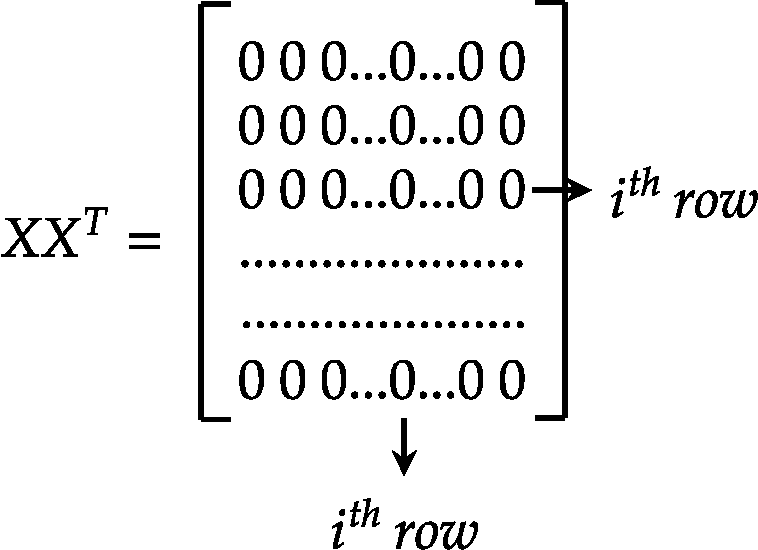
\includegraphics[height=4cm,width=6cm]{diagram-20210823(3)-crop}
		\end{figure}
		Since this matrix is diagonal, its eigenvalues are $a^{2}, 0,0 \ldots \ldots 0 .$ Hence, the number of non zero eigenvalues of the matrix $X X^{T}$ is 1 .\\\\
		So the correct answer is \textbf{Option (C)}
	\end{answer}
	\item The eigenvalues of a Hermitian matrix are all
	{\exyear{GATE 2018}}
	\begin{tasks}(4)
		\task[\textbf{A.}]  Real
		\task[\textbf{B.}] Imaginary
		\task[\textbf{C.}] Of modulus one
		\task[\textbf{D.}] Real and positive
	\end{tasks}
	\begin{answer}
		Eigenvalue of Hermitian matrix must be real.\\\\
		So the correct answer is \textbf{Option (A)}
	\end{answer}
	\item During a rotation, vectors along the axis of rotation remain unchanged. For the rotation matrix $\left(\begin{array}{ccc}0 & 1 & 0 \\ 0 & 0 & -1 \\ -1 & 0 & 0\end{array}\right)$, the vector along the axis of rotation is
	{\exyear{GATE 2019}}
	\begin{tasks}(2)
		\task[\textbf{A.}] $\frac{1}{3}(2 \hat{i}-\hat{j}+2 \hat{k})$
		\task[\textbf{B.}]  $\frac{1}{\sqrt{3}}(\hat{i}+\hat{j}-\hat{k})$
		\task[\textbf{C.}] $\frac{1}{\sqrt{3}}(\hat{i}-\hat{j}-\hat{k})$
		\task[\textbf{D.}] $\frac{1}{3}(2 \hat{i}+2 \hat{j}-\hat{k})$
	\end{tasks}
	\begin{answer}
		So the correct answer is \textbf{Option (B)}
	\end{answer}
\end{enumerate}
\colorlet{ocre1}{ocre!70!}
\colorlet{ocrel}{ocre!30!}
\setlength\arrayrulewidth{1pt}
\begin{table}[H]
	\centering
	\arrayrulecolor{ocre}
	\begin{tabular}{|p{1.5cm}|p{1.5cm}||p{1.5cm}|p{1.5cm}|}
		\hline
		\multicolumn{4}{|c|}{\textbf{Answer key}}\\\hline\hline
		\rowcolor{ocrel}Q.No.&Answer&Q.No.&Answer\\\hline
		1&\textbf{C} &2&\textbf{C}\\\hline 
		3&\textbf{D} &4&\textbf{C} \\\hline
		5&\textbf{B} &6&\textbf{5} \\\hline
		7&\textbf{D}&8&\textbf{C}\\\hline
		9&\textbf{A}&10&\textbf{B}\\\hline
		
	\end{tabular}
\end{table}
%\chapter{Power series Solution and Special functions}
\section{Series Solution Method}
Series expansion is a  method of obtaining one solution of the linear, second-order, homogeneous ODE. The method, will always work, provided the point of expansion is no worse than a regular singular point.In physics this very gentle condition is almost always satisfied. 
A linear, second-order, homogeneous ODE can be written in the form
\begin{equation}
\frac{d^{2} y}{d x^{2}}+P(x) \frac{d y}{d x}+Q(x) y=0 \label{DE002}
\end{equation}
The most general solution of the equation \ref{DE002} may be written as,
\begin{equation}
y(x)=c_{1} y_{1}(x)+c_{2} y_{2}(x)
\end{equation}
But a physical problem may lead to a nonhomogeneous, linear, second-order ODE
\begin{equation}
\frac{d^{2} y}{d x^{2}}+P(x) \frac{d y}{d x}+Q(x) y=F(x)\label{DE003}
\end{equation}
Hence the most general solution to the equation \label{DE003} will be of the form,
\begin{equation}
y(x)=c_{1} y_{1}(x)+c_{2} y_{2}(x)+y_{p}(x)
\end{equation}
The constants $c_{1}$ and $c_{2}$ will eventually be fixed by boundary conditions.\\\\
There are two series solution method  for differential equation,
\begin{enumerate}
	\item \textbf{Simple series expansion method}
	\item \textbf{Frobenious Method}
\end{enumerate}
\subsection{Simple Power Series Expansion Method}
The simple series expansion method works for differential equations whose solutions are well-behaved at the expansion point $x = 0$.
This method can be illustrated by Linear classical oscillator problem
\subsection{Classical Linear Oscillator}
\begin{align}
\frac{d^{2} y}{d x^{2}}+\omega^{2} y&=0 \label{DE003}\\
\text{with known solutions} \ y&=\sin \omega x, \cos \omega x\\
\text{We try}\ y(x) &=x^{k}\left(a_{0}+a_{1} x+a_{2} x^{2}+a_{3} x^{3}+\cdots\right) \\
&=\sum_{\lambda=0}^{\infty} a_{\lambda} x^{k+\lambda}, \quad a_{0} \neq 0 \label{DE004}\\
\intertext{with the exponent $k$ and all the coefficients $a_{\lambda}$ still undetermined. Note that $k$ need not be an integer. By differentiating twice, we obtain}
\frac{d y}{d x} &=\sum_{\lambda=0}^{\infty} a_{\lambda}(k+\lambda) x^{k+\lambda-1} \\
\frac{d^{2} y}{d x^{2}} &=\sum_{\lambda=0}^{\infty} a_{\lambda}(k+\lambda)(k+\lambda-1) x^{k+\lambda-2}
\intertext{By substituting into equation.\ref{DE003}, we have}
\sum_{\lambda=0}^{\infty} a_{\lambda}(k+\lambda)(k+\lambda-1) x^{k+\lambda-2}+\omega^{2} \sum_{\lambda=0}^{\infty} a_{\lambda} x^{k+\lambda}&=0 \label{DE005}
\intertext{The coefficients of each power of $x$ on the left-hand side of equation.\ref{DE005} must vanish individually.The lowest power of $x$ appearing in equation.\ref{DE005} is $x^{k-2}$, for $\lambda=0$ in the first summation. The requirement that the coefficient vanish  yields,}
a_{0} k(k-1)&=0
\intertext{We had chosen $a_{0}$ as the coefficient of the lowest nonvanishing terms of the series \ref{DE004}, hence, by definition, $a_{0} \neq 0$. Therefore we have,}
k(k-1)&=0 \label{DE006}
\end{align}
\textbf{This equation, coming from the coefficient of the lowest power of $x$, we call the {indicial equation}.} The indicial equation and its roots are of critical importance to our analysis.
\\From equation.\ref{DE006}, \qquad $k=0 $ or $k=1$\\
The only way a power series can be zero is, it's coefficients must be equal to zero. But here the power of $x$ in the equation do not match up. The Coefficent of $x$ in the first term is,${k+\lambda-2} $ and for the second term it is,$k+\lambda$, to make them equal, we can replace $\lambda$ by $\lambda+2$ in the first term. Then we get,
\begin{align}
\sum_{\lambda=2}^{\infty} a_{\lambda+2}(k+\lambda+2)(k+\lambda+1) x^{k+\lambda}+\omega^{2} \sum_{\lambda=0}^{\infty} a_{\lambda} x^{k+\lambda}&=0\\
\sum_{\lambda=2}^{\infty} a_{\lambda+2}(k+\lambda+2)(k+\lambda+1) +\omega^{2} \sum_{\lambda=0}^{\infty} a_{\lambda} &=0
\intertext{Here the coefficients  are independent summations and $\lambda $ is a dummy index. Then we get,}
a_{\lambda+2}(k+\lambda+2)(k+\lambda+1) +\omega^{2} a_{\lambda} &=0\\
a_{\lambda+2}&=-a_{\lambda} \frac{\omega^{2}}{(k+\lambda+2)(k+\lambda+1)}\label{DE007}
\end{align}
For this example, if we start with $a_{0}$, Equation.\ref{DE007} leads to the even coefficients $a_{2}, a_{4}$, and so on, and ignores $a_{1}, a_{3}, a_{5}$, and so on. Since $a_{1}$ is arbitrary if $k=0$ and necessarily zero if $k=1$, 
$$
a_{3}=a_{5}=a_{7}=\cdots=0
$$
and all the odd-numbered coefficients vanish. The odd powers of $x$ will actually reappear when the second root of the indicial equation is used.
\begin{align}
a_{\lambda+2}&=-a_{\lambda} \frac{\omega^{2}}{(\lambda+2)(\lambda+1)}
\intertext{which leads to}
a_{2}&=-a_{0} \frac{\omega^{2}}{1 \cdot 2}=-\frac{\omega^{2}}{2 !} a_{0} \\
a_{4}&=-a_{2} \frac{\omega^{2}}{3 \cdot 4}=+\frac{\omega^{4}}{4 !} a_{0} \\
a_{6}&=-a_{4} \frac{\omega^{2}}{5 \cdot 6}=-\frac{\omega^{6}}{6 !} a_{0}, \quad \text { and so on. }
\intertext{By inspection (and mathematical induction),}
a_{2 n}&=(-1)^{n} \frac{\omega^{2 n}}{(2 n) !} a_{0}
\intertext{and our solution is}
y(x)_{k=0}&=a_{0}\left[1-\frac{(\omega x)^{2}}{2 !}+\frac{(\omega x)^{4}}{4 !}-\frac{(\omega x)^{6}}{6 !}+\cdots\right]\\&=a_{0} \cos \omega x\\
\intertext{If we choose the indicial equation root $k=1$ Equation.\ref{DE007}, the recurrence relation becomes}
a_{j+2}&=-a_{j} \frac{\omega^{2}}{(j+3)(j+2)}\\
\intertext{Substituting in $j=0,2,4$, successively, we obtain}
a_{2}=-a_{0} \frac{\omega^{2}}{2 \cdot 3}&=-\frac{\omega^{2}}{3 !} a_{0} \\
a_{4}=-a_{2} \frac{\omega^{2}}{4 \cdot 5}&=+\frac{\omega^{4}}{5 !} a_{0} \\
a_{6}=-a_{4} \frac{\omega^{2}}{6 \cdot 7}&=-\frac{\omega^{6}}{7 !} a_{0}, \quad \text { and so on. }
\intertext{Again, by inspection and mathematical induction,}
a_{2 n}&=(-1)^{n} \frac{\omega^{2 n}}{(2 n+1) !} a_{0}\\
\intertext{For this choice, $k=1$, we obtain}
y(x)_{k=1} &=a_{0} x\left[1-\frac{(\omega x)^{2}}{3 !}+\frac{(\omega x)^{4}}{5 !}-\frac{(\omega x)^{6}}{7 !}+\cdots\right] \\
&=\frac{a_{0}}{\omega}\left[(\omega x)-\frac{(\omega x)^{3}}{3 !}+\frac{(\omega x)^{5}}{5 !}-\frac{(\omega x)^{7}}{7 !}+\cdots\right] \\
&=\frac{a_{0}}{\omega} \sin \omega x
\end{align}
\subsubsection{Power Series Solution (About an Ordinary Point)}
Find the power series solution of $\left(1-x^{2}\right) y^{\prime \prime}-2 x y^{\prime}+2 y=0$ about $x=0$\\\\
Since $x=0$ is an ordinary point of the given differential equation, the solution can be written as
\begin{align*}
y&=\sum_{k=0}^{\infty} a_{k} x^{k} \\ \frac{d y}{d x}&=\sum_{k=0}^{\infty} k a_{k} x^{k-1} \\ \frac{d^{2} y}{d x^{2}}&=\sum_{k=0}^{\infty} a_{k} k(k-1) x^{k-2}
\intertext{Substituting these values in the given equation we get,}
\left(1-x^{2}\right) \sum_{k} a_{k} k(k-1) x^{k-2}&-2 x \sum_{k} a_{k}(k) x^{k-1}+2 \sum_{k} a_{k} x^{k}=0 \\
\sum_{k=2} a_{k} k(k-1) x^{k-2}&-\sum\left(k^{2}+k-2\right) a_{k} x^{k}=0
\intertext{now equating the coefficient of $x^{k}$ then}
(k+2)(k+1) a_{k+2}-\left(k^{2}+k-2\right) a_{k}&=0 \\a_{k+2}&=\frac{k-1}{(k+1)} a_{k}\\
\text{For} \ k&=0 \Rightarrow a_{2}=-a_{0} \\ k&=1 \Rightarrow a_{3}=0 \\
k&=2 \Rightarrow a_{4}=\frac{a_{2}}{3}=\frac{-a_{0}}{3}  \\ k&=3 \Rightarrow a_{5}=\frac{2}{4} a_{3}=0\\
\text{Therefore, solution}\ y&=a_{0}+a_{1} x+a_{2} x^{2}+\ldots \ldots\\&=a_{0}\left[1-x^{2}-\frac{x^{4}}{3} \ldots . .\right]+a_{1} x
\end{align*}
\subsection{Frobenious Method}
Even though the simple power series expansion method works for many functions there are some whose behaviour  precludes the simple series method like the Bessel's function. The need of Frobenious method  lies under the fact that, \textbf{any functions involving negative or fractional powers would not be amenable to power series solution method}. The Frobenious method extends the simple power series solution method to include negative and fractional powers, and it also allows a natural extension involving logarithm terms.\\
The basic idea of the Frobenius method is to look for solutions of the form
\begin{align*}
y(x) &=a_{0} x^{\lambda}+a_{1} x^{\lambda+1}+a_{2} x^{\lambda+2}+a_{3} x^{\lambda+3}+\ldots \\
&=x^{\lambda}\left(a_{0}+a_{1} x+a_{2} x^{2}+a_{3} x^{3}+\ldots\right) \\
&=x^{\lambda} \sum_{k=0}^{\infty} a_{k} x^{k} \\
&= \sum_{k=0}^{\infty} a_{k} x^{k+\lambda}
\end{align*}
The extension of the simple power series method is all in the factor $x^{\lambda}$. The power $c$ must now be determined, as well as the coefficients $a_{k}$. Since $\lambda$ may be negative, positive, and possibly non-integral, this extends considerably the range of functions which may be treated. Note that $a_{0}$ is the lowest non-zero coefficient, so by definition it cannot be zero.
\subsection{Bessel Function}
\newpage
\begin{abox}
	Problem Set -1
\end{abox}
\begin{enumerate}[label=\color{ocre}\textbf{\arabic*.}]
	\item  Let $p_{n}(x)$ (where $n=0,1,2, \ldots \ldots$ ) be a polynomial of degree $n$ with real coefficients, defined in the interval $2 \leq n \leq 4$. If $\int_{2}^{4} p_{n}(x) p_{m}(x) d x=\delta_{n m}$, then
	{\exyear{NET/JRF(JUNE-2011)}}
	\begin{tasks}(2)
		\task[\textbf{A.}] $p_{0}(x)=\frac{1}{\sqrt{2}}$ and $p_{1}(x)=\sqrt{\frac{3}{2}}(-3-x)$
		\task[\textbf{B.}]  $p_{0}(x)=\frac{1}{\sqrt{2}}$ and $p_{1}(x)=\sqrt{3}(3+x)$
		\task[\textbf{C.}] $p_{0}(x)=\frac{1}{2}$ and $p_{1}(x)=\sqrt{\frac{3}{2}}(3-x)$
		\task[\textbf{D.}] $p_{0}(x)=\frac{1}{\sqrt{2}}$ and $p_{1}(x)=\sqrt{\frac{3}{2}}(3-x)$
	\end{tasks}
	\item  The generating function $F(x, t)=\sum_{n=0}^{\infty} P_{n}(x) t^{n}$ for the Legendre polynomials $P_{n}(x)$ is $F(x, t)=\left(1-2 x t+t^{2}\right)^{-1 / 2}$. The value of $P_{3}(-1)$ is
	{\exyear{NET/JRF(DEC-2011)}}
	\begin{tasks}(4)
		\task[\textbf{A.}] $5 / 2$
		\task[\textbf{B.}] $3 / 2$
		\task[\textbf{C.}] $+1$
		\task[\textbf{D.}] $-1$
	\end{tasks}
	\item  The graph of the function $f(x)$ shown below is best described by
	{\exyear{NET/JRF(DEC-2012)}}
	\begin{figure}[H]
		\centering
		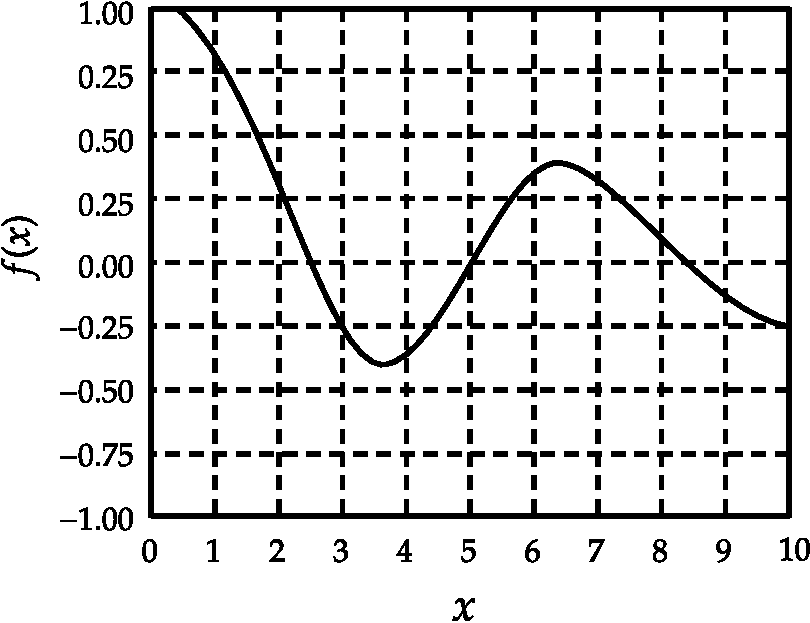
\includegraphics[height=6cm,width=8cm]{diagram-20211005(12)-crop}
	\end{figure}
	\begin{tasks}(2)
		\task[\textbf{A.}]  The Bessel function $J_{0}(x)$
		\task[\textbf{B.}] $\cos x$
		\task[\textbf{C.}] $e^{-x} \cos x$
		\task[\textbf{D.}] $\frac{1}{x} \cos x$
	\end{tasks}
	\item Given that $\sum_{n=0}^{\infty} H_{n}(x) \frac{t^{n}}{n !}=e^{-t^{2}+2 t x}$ the value of $H_{4}(0)$ is
	{\exyear{NET/JRF(JUNE-2013)}}
	\begin{tasks}(4)
		\task[\textbf{A.}] 12
		\task[\textbf{B.}] 6
		\task[\textbf{C.}] 24
		\task[\textbf{D.}] $-6$
	\end{tasks}
	\item   Given $\sum_{n=0}^{\infty} P_{n}(x) t^{n}=\left(1-2 x t+t^{2}\right)^{-1 / 2}$, for $|t|<1$, the value of $P_{5}(-1)$ is
	{\exyear{NET/JRF(JUNE-2014)}}
	\begin{tasks}(4)
		\task[\textbf{A.}] $0.26$
		\task[\textbf{B.}] 1
		\task[\textbf{C.}] $0.5$
		\task[\textbf{D.}] $-1$
	\end{tasks}
	\item The function $f(x)=\sum_{n=0}^{\infty} \frac{(-1)^{n}}{n !(n+1) !}\left(\frac{x}{2}\right)^{2 n+1}$, satisfies the differential equation
	{\exyear{NET/JRF(DEC-2014)}}
	\begin{tasks}(2)
		\task[\textbf{A.}]  $x^{2} \frac{d^{2} f}{d x^{2}}+x \frac{d f}{d x}+\left(x^{2}+1\right) f=0$
		\task[\textbf{B.}]  $x^{2} \frac{d^{2} f}{d x^{2}}+2 x \frac{d f}{d x}+\left(x^{2}-1\right) f=0$
		\task[\textbf{C.}] $x^{2} \frac{d^{2} f}{d x^{2}}+x \frac{d f}{d x}+\left(x^{2}-1\right) f=0$
		\task[\textbf{D.}] $x^{2} \frac{d^{2} f}{d x^{2}}-x \frac{d f}{d x}+\left(x^{2}-1\right) f=0$
	\end{tasks}
	\item
	 The Hermite polynomial $H_{n}(x)$, satisfies the differential equation
	$$
	\frac{d^{2} H_{n}}{d x^{2}}-2 x \frac{d H_{n}}{d x}+2 n H_{n}(x)=0
	$$
	The corresponding generating function $G(t, x)=\sum_{n=0}^{\infty} \frac{1}{n !} H_{n}(x) t^{n}$, satisfies the equation
	{\exyear{NET/JRF(DEC-2015)}}
	\begin{tasks}(2)
		\task[\textbf{A.}] $\frac{\partial^{2} G}{\partial x^{2}}-2 x \frac{\partial G}{\partial x}+2 t \frac{\partial G}{\partial t}=0$
		\task[\textbf{B.}] $\frac{\partial^{2} G}{\partial x^{2}}-2 x \frac{\partial G}{\partial x}-2 t^{2} \frac{\partial G}{\partial t}=0$
		\task[\textbf{C.}] $\frac{\partial^{2} G}{\partial x^{2}}-2 x \frac{\partial G}{\partial x}+2 \frac{\partial G}{\partial t}=0$
		\task[\textbf{D.}]  $\frac{\partial^{2} G}{\partial x^{2}}-2 x \frac{\partial G}{\partial x}+2 \frac{\partial^{2} G}{\partial x \partial t}=0$
	\end{tasks}
	\item A stable asymptotic solution of the equation $x_{n+1}=1+\frac{3}{1+x_{n}}$ is $x=2$. If we take $x_{n}=2+\epsilon_{n}$ and $x_{n+1}=2+\epsilon_{n+1}$, where $\epsilon_{n}$ and $\epsilon_{n+1}$ are both small, the ratio $\frac{\epsilon_{n+1}}{\epsilon_{n}}$ is approximately
	{\exyear{NET/JRF(DEC-2016)}}
	\begin{tasks}(4)
		\task[\textbf{A.}] $-\frac{1}{2}$
		\task[\textbf{B.}] $-\frac{1}{4}$
		\task[\textbf{C.}]  $-\frac{1}{3}$
		\task[\textbf{D.}] $-\frac{2}{3}$
	\end{tasks}
	\item  The Green's function satisfying
	$$
	\frac{d^{2}}{d x^{2}} g\left(x, x_{0}\right)=\delta\left(x-x_{0}\right)
	$$
	with the boundary conditions $g\left(-L, x_{0}\right)=0=g\left(L, x_{0}\right)$, is
	{\exyear{NET/JRF(JUNE-2017)}}
	\begin{tasks}(1)
		\task[\textbf{A.}] $\left\{\begin{array}{ll}\frac{1}{2 L}\left(x_{0}-L\right)(x+L), & -L \leq x<x_{0} \\ \frac{1}{2 L}\left(x_{0}+L\right)(x-L), & x_{0} \leq x \leq L\end{array}\right.$
		\task[\textbf{B.}]  $\left\{\begin{array}{ll}\frac{1}{2 L}\left(x_{0}+L\right)(x+L), & -L \leq x<x_{0} \\ \frac{1}{2 L}\left(x_{0}-L\right)(x-L), & x_{0} \leq x \leq L\end{array}\right.$
		\task[\textbf{C.}] $\left\{\begin{array}{ll}\frac{1}{2 L}\left(L-x_{0}\right)(x+L), & -L \leq x<x_{0} \\ \frac{1}{2 L}\left(x_{0}+L\right)(L-x), & x_{0} \leq x \leq L\end{array}\right.$
		\task[\textbf{D.}] $\frac{1}{2 L}(x-L)(x+L), \quad-L \leq x \leq L$
	\end{tasks}
	\item  The generating function $G(t, x)$ for the Legendre polynomials $P_{n}(t)$ is
	$$
	G(t, x)=\frac{1}{\sqrt{1-2 x t+x^{2}}}=\sum_{n=0}^{\infty} x^{n} P_{n}(t), \text { for }|x|<1
	$$
	If the function $f(x)$ is defined by the integral equation $\int_{0}^{x} f\left(x^{\prime}\right) d x^{\prime}=x G(1, x)$, it can be expressed as
	{\exyear{NET/JRF(DEC-2017)}}
	\begin{tasks}(2)
		\task[\textbf{A.}] $\sum_{n, m=0}^{\infty} x^{n+m} P_{n}(1) P_{m}\left(\frac{1}{2}\right)$
		\task[\textbf{B.}] $\sum_{n, m=0}^{\infty} x^{n+m} P_{n}(1) P_{m}(1)$
		\task[\textbf{C.}] $\sum_{n, m=0}^{\infty} x^{n-m} P_{n}(1) P_{m}(1)$
		\task[\textbf{D.}] $\sum_{n, m=0}^{\infty} x^{n-m} P_{n}(0) P_{m}(1)$
	\end{tasks}
	\item In the function $P_{n}(x) e^{-x^{2}}$ of a real variable $x, P_{n}(x)$ is polynomial of degree $n$. The maximum number of extrema that this function can have is
	{\exyear{NET/JRF(JUNE-2018)}}
	\begin{tasks}(4)
		\task[\textbf{A.}] $n+2$
		\task[\textbf{B.}]  $n-1$
		\task[\textbf{C.}] $n+1$
		\task[\textbf{D.}] $n$
	\end{tasks}
	\item  The Green's function $G\left(x, x^{\prime}\right)$ for the equation $\frac{d^{2} y(x)}{d x^{2}}+y(x)=f(x)$, with the boundary values $y(0)=y\left(\frac{\pi}{2}\right)=0$, is
	{\exyear{NET/JRF(JUNE-2018)}}
	\begin{tasks}(1)
		\task[\textbf{A.}] $G\left(x, x^{\prime}\right)=\left\{\begin{array}{ll}x\left(x^{\prime}-\frac{\pi}{2}\right), & 0<x<x^{\prime}<\frac{\pi}{2} \\ \left(x-\frac{\pi}{2}\right) x^{\prime}, & 0<x^{\prime}<x<\frac{\pi}{2}\end{array}\right.$
		\task[\textbf{B.}] $G\left(x, x^{\prime}\right)=\left\{\begin{array}{ll}-\cos x^{\prime} \sin x, & 0<x<x^{\prime}<\frac{\pi}{2} \\ -\sin x^{\prime} \cos x, & 0<x^{\prime}<x<\frac{\pi}{2}\end{array}\right.$
		\task[\textbf{C.}] $G\left(x, x^{\prime}\right)=\left\{\begin{array}{ll}\cos x^{\prime} \sin x, & 0<x<x^{\prime}<\frac{\pi}{2} \\ \sin x^{\prime} \cos x, & 0<x^{\prime}<x<\frac{\pi}{2}\end{array}\right.$
		\task[\textbf{D.}] $G\left(x, x^{\prime}\right)=\left\{\begin{array}{ll}x\left(\frac{\pi}{2}-x^{\prime}\right), & 0<x<x^{\prime}<\frac{\pi}{2} \\ x^{\prime}\left(\frac{\pi}{2}-x\right), & 0<x^{\prime}<x<\frac{\pi}{2}\end{array}\right.$
	\end{tasks}
	\item The polynomial $f(x)=1+5 x+3 x^{2}$ is written as linear combination of the Legendre polynomials
	$\left(P_{0}(x)=1, P_{1}(x), P_{2}(x)=\frac{1}{2}\left(3 x^{2}-1\right)\right)$ as $f(x)=\sum_{n} c_{n} P_{n}(x)$. The value of $c_{0}$ is
	{\exyear{NET/JRF(DEC-2018)}}
	\begin{tasks}(4)
		\task[\textbf{A.}] $\frac{1}{4}$
		\task[\textbf{B.}] $\frac{1}{2}$
		\task[\textbf{C.}]  2
		\task[\textbf{D.}]  4
	\end{tasks}
	\item The Green's function $G\left(x, x^{\prime}\right)$ for the equation $\frac{d^{2} y(x)}{d x^{2}}=f(x)$, with the boundary values $y(0)=0$ and $y(1)=0$, is
	{\exyear{NET/JRF(DEC-2018)}}
	\begin{tasks}(1)
		\task[\textbf{A.}] $G\left(x, x^{\prime}\right)=\left\{\begin{array}{ll}\frac{1}{2} x\left(1-x^{\prime}\right), & 0<x<x^{\prime}<1 \\ \frac{1}{2} x^{\prime}(1-x) & 0<x^{\prime}<x<1\end{array}\right.$
		\task[\textbf{B.}] $G\left(x, x^{\prime}\right)=\left\{\begin{array}{ll}x\left(x^{\prime}-1\right), & 0<x<x^{\prime}<1 \\ x^{\prime}(1-x) & 0<x^{\prime}<x<1\end{array}\right.$
		\task[\textbf{C.}] $G\left(x, x^{\prime}\right)=\left\{\begin{array}{ll}-\frac{1}{2} x\left(1-x^{\prime}\right), & 0<x<x^{\prime}<1 \\ \frac{1}{2} x^{\prime}(1-x) & 0<x^{\prime}<x<1\end{array}\right.$
		\task[\textbf{D.}]  $G\left(x, x^{\prime}\right)=\left\{\begin{array}{ll}x\left(x^{\prime}-1\right), & 0<x<x^{\prime}<1 \\ x^{\prime}(x-1) & 0<x^{\prime}<x<1\end{array}\right.$
	\end{tasks}
	\item  The Green's function for the differential equation $\frac{d^{2} x}{d t^{2}}+x=f(t)$, satisfying the initial conditions $x(0)=\frac{d x}{d t}(0)=0$ is\\
	$$G(t, \tau)=\left\{\begin{array}{ll}0 & \text { for } \quad 0<t<\tau \\ \sin (t-\tau) & \text { for } \quad t>\tau\end{array}\right.$$\\
	The solution of the differential equation when the source $f(t)=\theta(t)$ (the Heaviside step function) is
	{\exyear{NET/JRF(JUNE-2020)}}
	\begin{tasks}(4)
		\task[\textbf{A.}] $\sin t$
		\task[\textbf{B.}] $1-\sin t$
		\task[\textbf{C.}] $1-\cos t$
		\task[\textbf{D.}] $\cos ^{2} t-1$
	\end{tasks}
\end{enumerate}
 \colorlet{ocre1}{ocre!70!}
\colorlet{ocrel}{ocre!30!}
\setlength\arrayrulewidth{1pt}
\begin{table}[H]
	\centering
	\arrayrulecolor{ocre}
	\begin{tabular}{|p{1.5cm}|p{1.5cm}||p{1.5cm}|p{1.5cm}|}
		\hline
		\multicolumn{4}{|c|}{\textbf{Answer key}}\\\hline\hline
		\rowcolor{ocrel}Q.No.&Answer&Q.No.&Answer\\\hline
		1&\textbf{D} &2&\textbf{D}\\\hline 
		3&\textbf{A} &4&\textbf{A} \\\hline
		5&\textbf{D} &6&\textbf{C} \\\hline
		7&\textbf{A}&8&\textbf{C}\\\hline
		9&\textbf{A}&10&\textbf{B}\\\hline
		11&\textbf{C} &12&\textbf{B}\\\hline
		13&\textbf{C}&14&\textbf{D}\\\hline
		15&\textbf{C}& &\\\hline
		
	\end{tabular}
\end{table}
\begin{abox}
	Problem Set -3
\end{abox}
\begin{enumerate}[label=\color{ocre}\textbf{\arabic*.}]
	\item Green function for time dependent Schrödinger wave equation is defined as $G\left(\vec{r}, t: r^{\prime}, t^{\prime}\right)$. If $H$ is Hamiltonion of system then $G\left(\vec{r}, t: r^{\prime}, t^{\prime}\right)$ will satisfied the equation
	 \begin{tasks}(1)
		\task[\textbf{a.}]$\left(i \hbar \frac{\partial}{\partial t}-H\right) G\left(\vec{r}, t ; \vec{r}^{\prime}, t^{\prime}\right)=0$
		\task[\textbf{b.}]$\left(i \hbar \frac{\partial}{\partial t}-H\right) G\left(\vec{r}, t ; \vec{r}^{\prime}, t^{\prime}\right)=\delta\left(\vec{r}-\vec{r}^{\prime}\right)$
		\task[\textbf{c.}] $\left(i \hbar \frac{\partial}{\partial t}-H\right) G\left(\vec{r}, t ; \vec{r}^{\prime}, t^{\prime}\right)=\delta\left(t-t^{\prime}\right)$
		\task[\textbf{d.}]  $\left(i \hbar \frac{\partial}{\partial t}-H\right) G\left(\vec{r}, t ; \vec{r}^{\prime}, t^{\prime}\right)=\delta\left(\vec{r}-\vec{r}^{\prime}\right) \delta\left(t-t^{\prime}\right)$
	\end{tasks}
\begin{answer}
So the correct answer is \textbf{Option (d)}
\end{answer}
	\item $G\left(x, x_{0}\right)$ is the Green's function associated with the boundary value problem consisting of ordinary differential equation.
	$$
	\frac{d}{d x}\left(p(x) \frac{d u}{d x}\right)=f(x) \text { with } u(0)=0, u(L)=0
	$$
	The discontinuity condition on the derivative $\frac{d G\left(x, x_{0}\right)}{d x}$ at $x=x_{0}$ is
	 \begin{tasks}(4)
		\task[\textbf{a.}]0
		\task[\textbf{b.}]$p\left(x_{0}\right)$
		\task[\textbf{c.}]1
		\task[\textbf{d.}] $\frac{1}{p\left(x_{0}\right)}$
	\end{tasks}
\begin{answer}
	\begin{align*}
	\left.\frac{d G}{d x}\right|_{x=x_{0}^{+}}-\left.\frac{d G}{d x}\right|_{x=x_{i 1}^{-}}=\frac{1}{p\left(x_{0}\right)}
	\end{align*}
	So the correct answer is \textbf{Option (d)}
\end{answer}
\item Consider the steady state heat equation $\frac{d^{2} u}{d x^{2}}=f(x)$ with boundary condition,
$$
u(0)=0, u(L)=0
$$
The Green's function associated with the above equation
 \begin{tasks}(2)
	\task[\textbf{a.}]Constant
	\task[\textbf{b.}] Linear function
	\task[\textbf{c.}] Parabolic function
	\task[\textbf{d.}] Hyperbolic function
\end{tasks}
\begin{answer}
	\begin{align*}
	\intertext{The Green's function satisfies}
	\frac{d^{2} G\left(x, x_{0}\right)}{d x^{2}}&=\delta\left(x-x_{0}\right)\\
\text{	with }G\left(0, x_{0}\right)&=0\text{ and }G\left(L, x_{0}\right)=0
\intertext{Corresponding homogeneous equation is:}
\frac{d^{2} G}{d x^{2}}&=0\\
\text{Solution for }x \neq x_{0}&\text{ are, }G\left(x, x_{0}\right)= \begin{cases}a+b x_{2} & x<x_{1+} \\ c+d x, & x>x_{0}\end{cases}
	\end{align*}
		So the correct answer is \textbf{Option (b)}
\end{answer}
\item Consider the steady state heat equation $\frac{d^{2} u}{d x^{2}}=f(x)$ with boundary condition. $u(0)=0, u(L)=0$
The Green's function associated with the above equation is
 \begin{tasks}(1)
	\task[\textbf{a.}] $G\left(x, x_{0}\right)= \begin{cases}\frac{x}{L}\left(x_{0}-L\right), & 0 \leq x \leq x_{0} \\ \frac{x_{0}}{L}(x-L), & x_{0} \leq x \leq L\end{cases}$
	\task[\textbf{b.}] $G\left(x, x_{0}\right)= \begin{cases}\frac{x}{L}\left(L-x_{0}\right), & 0 \leq x \leq x_{0} \\ \frac{x_{0}}{L}(L-x), & x_{0} \leq x \leq L\end{cases}$
	\task[\textbf{c.}] $G\left(x, x_{0}\right)= \begin{cases}\sqrt{\frac{x}{L},} &\quad 0 \leq x \leq x_{0} \\ \sqrt{\frac{(x-L)}{L}}, & \quad x_{0} \leq x \leq L\end{cases}$
	\task[\textbf{d.}] $G\left(x, x_{0}\right)= \begin{cases}\sqrt{\frac{L-x}{L},}, & 0 \leq x \leq x_{0} \\ \sqrt{\frac{(x)}{L}}, & x_{0} \leq x \leq L\end{cases}$
\end{tasks}
\begin{answer}
	\begin{align*}
	\intertext{The Green's function satisfies}
	\frac{d^{2} G\left(x, x_{0}\right)}{d x^{2}}&=\delta\left(x-x_{0}\right)\\
	\text{with }G\left(0, x_{0}\right)&=0\text{ and }G\left(L, x_{0}\right)=0
	\intertext{Corresponding homogeneous equation is:}
	\frac{d^{2} G}{d x^{2}}&=0\\
	\text{Solution for }&x \neq x_{0}\text{ are}\\
	G\left(x, x_{0}\right)&= \begin{cases}a+b x, & x<x_{0} \\ c+d x, & x>x_{0}\end{cases}
	\intertext{From boundary conditions:}
	G\left(0, x_{0}\right)&=0 \Rightarrow a=0\\
	G\left(L, x_{0}\right)&=0 \Rightarrow c=-d L\\
	\therefore G\left(x, x_{0}\right)&= \begin{cases}b x, & x<x_{0} \\ d(x-L), & x>x_{0}\end{cases}\\
	\text{From continuity of }&\text{Green's function at }x=x_{0},\text{ we have}\\
	b x_{0}&=d\left(x_{0}-L\right)\\
	b&=\frac{d\left(x_{0}-L\right)}{x_{0}}\\
	\text{From discontinuity of }&\frac{\partial G}{\partial x}\text{ at }x=x_{0}\text{, we have}\\
	\left.\frac{\partial G}{\partial x}\right|&_{x=x_{0}^{+}}-\left.\frac{\partial G}{\partial x}\right|_{x=x_{0}^{-}}=1\\
	d-b&=1\\
	\Rightarrow d&=b+1 \Rightarrow d=\frac{d\left(x_{0}-L\right)}{x_{0}}+1 \Rightarrow d x_{0}=d x_{0}-d L+x_{0}\\
	\Rightarrow d&=\frac{x_{0}}{L}, b=d-1=\left(\frac{x_{0}}{L}-1\right)\\
	\therefore G\left(x, x_{0}\right)&= \begin{cases}\frac{x}{L}\left(x_{0}-L\right), & 0 \leq x \leq x_{0} \\ \frac{x_{0}}{L}(x-L), & x_{0} \leq x \leq L\end{cases}
	\end{align*}
		So the correct answer is \textbf{Option (a)}
\end{answer}
\item The differential equation defined as $\frac{d^{2} y}{d x^{2}}=f(x)$ With boundary conditions $\quad y(0)=0$ and $y^{\prime}(1)=0$
The green function $G\left(x, x_{0}\right)$ satisfy the
 \begin{tasks}(2)
	\task[\textbf{a.}]$G\left(x, x_{0}\right)= \begin{cases}x & \text { if } x<x_{0} \\ x_{0} & \text { if } x>x_{0}\end{cases}$
	\task[\textbf{b.}]$G\left(x, x_{0}\right)= \begin{cases}-x & \text { if } x<x_{0} \\ -x_{0} & \text { if } x>x_{0}\end{cases}$
	\task[\textbf{c.}]$G\left(x, x_{0}\right)= \begin{cases}x^{2} & \text { if } x<x_{0} \\ -x_{0} & \text { if } x>x_{0}\end{cases}$
	\task[\textbf{d.}] $G\left(x, x_{0}\right)= \begin{cases}-x^{2} & \text { if } x<x_{0} \\ -x_{0} & \text { if } x>x_{0}\end{cases}$
\end{tasks}
\begin{answer}
	\begin{align}
	\intertext{The corresponding non-homogenous differential equation for Green's function is}\notag\\
	\frac{\partial^{2}}{\partial x^{2}} G\left(x, x_{0}\right)&=\delta\left(x-x_{0}\right)\\
	\text{With }G\left(0, x_{0}\right)&=0\text{ and }G^{\prime}\left(1, x_{0}\right)=0\notag\notag\\
\text{	Let }&\frac{\partial^{2}}{\partial x^{2}} G\left(x, x_{0}\right)=0\notag\\
\Rightarrow G\left(x, x_{0}\right)&= \begin{cases}A x+B, & x<x_{0} \\ C x+D, & x>x_{0}\end{cases}\label{SF-01}
\intertext{Using booundary condition, we have}\notag\\
B&=0\text{ and }C=0\notag\\
\therefore&\text{ equation (\ref{SF-01}) becomes}\notag\\
G\left(x, x_{b}\right)&= \begin{cases}A x, & x<x_{0} \\ D, & x>x_{i 1}\end{cases}\notag\\
\text{From continuity of }&\left(f\left(x, x_{0}\right)\right.\text{ at }x=x_{0}\text{, we have}\notag\\
A x_{0}&=D
\intertext{From discontinuity of first derivative of Green's function i.c. $\frac{\partial G}{\partial x}$ at $x=x_{0}$ we have}
\left.\frac{\partial G}{\partial x}\right|_{x=x_{0}^{+}}-\left.\frac{\partial G}{\partial x}\right|&_{x=x_{0}^{-}}=1\notag\\
\Rightarrow 0-A&=1 \Rightarrow A=-1\notag\\
\text{and }D&=-x_{0}\notag\\
\therefore G\left(x, x_{0}\right)&= \begin{cases}-x & \text { if } x<x_{0} \notag\\ -x_{0} & \text { if } x>x_{0}\end{cases}
	\end{align}
	So the correct answer is \textbf{Option (b)}
\end{answer}
\item For real $n$ the cylindrical Bessel function of order $n$ is $J_{n}(x)$ then $J_{1 / 2}$ will converge to
 \begin{tasks}(4)
	\task[\textbf{a.}]0
	\task[\textbf{b.}]1
	\task[\textbf{c.}] $-1$
	\task[\textbf{d.}] $\frac{1}{2}$
\end{tasks}
\begin{answer}
	\begin{align*}
	{{\color{red}{Not completed}}}\\
	\end{align*}
	So the correct answer is \textbf{Option (a)}
\end{answer}
\item For real $n$ the cylindrical Bessel function is $J_{n}(x)$ of order $n$ then behavior $J_{1 / 2}$ will behave $x \approx 0$ as
 \begin{tasks}(4)
	\task[\textbf{a.}] 0
	\task[\textbf{b.}]$\sqrt{\frac{2 x}{\pi}}$
	\task[\textbf{c.}]$\sqrt{\frac{x}{\pi}}$
	\task[\textbf{d.}]  $\sqrt{\frac{x}{2 \pi}}$
\end{tasks}
\begin{answer}
	\begin{align*}
	{{\color{red}{Not completed}}}\\
	J_{n}(x)&=\sum_{0}^{\infty} \frac{(-1)^{r}}{[r \mid n+r}\left(\frac{x}{2}\right)^{n+2 r} \Rightarrow J_{1 / 2}(x)=\sum_{0}^{\infty} \frac{(-1)^{r}}{\left\lfloor\frac{1}{2}+r\right.}\left(\frac{x}{2}\right)^{\frac{1}{2}+2 r}\\
	\text{Put }r&=0 \frac{\sqrt{x / 2}}{\frac{1}{2}}=\sqrt{\frac{2 x}{\pi}} \text{where }\frac{1}{2}=\frac{\sqrt{\pi}}{2}
	\end{align*}
		So the correct answer is \textbf{Option (b)}
\end{answer}
\item For real $n$ the cylindrical Bessel function is $J_{n}(x)$ of order $n$ then behavior $J_{1 / 2}$ will equivalent to (it is given that $\underline{r} \cdot\left\lfloor r-\frac{1}{2}=\left[(2 r) 2^{-r} \sqrt{\pi}\right)\right.$
 \begin{tasks}(4)
	\task[\textbf{a.}] $\sqrt{\frac{2}{\pi}} \frac{\sin x}{\sqrt{x}}$
	\task[\textbf{b.}]$\sqrt{\frac{2}{\pi}} \frac{\sin x}{x}$
	\task[\textbf{c.}]$\sqrt{\frac{2}{\pi}} \frac{\cos x}{\sqrt{x}}$
	\task[\textbf{d.}] $\sqrt{\frac{2}{\pi}} \frac{\cos }{x}$
\end{tasks} 
\begin{answer}
	\begin{align*}
	{{\color{red}{Not completed}}}\\
	\end{align*}
\end{answer}
\item For real $n$ the cylindrical Bessel function is $J_{n}(x)$ of order $n$ then $J_{n}(x)$ will satisfied differential equation
 \begin{tasks}(1)
	\task[\textbf{a.}]$\frac{d^{2} J_{n}}{d x^{2}}+\frac{1}{x}\left(\frac{d J_{n}}{d x}\right)+\left(1+\frac{n^{2}}{x^{2}}\right) J_{n}=0$
	\task[\textbf{b.}] $\frac{d^{2} J_{n}}{d x^{2}}+\frac{1}{x}\left(\frac{d J_{n}}{d x}\right)+\left(1-\frac{n^{2}}{x^{2}}\right) J_{n}=0$
	\task[\textbf{c.}] $\frac{d^{2} J_{n}}{d x^{2}}+x\left(\frac{d J_{n}}{d x}\right)+\left(1+\frac{n^{2}}{x^{2}}\right) J_{n}=0$
	\task[\textbf{d.}] $\frac{d^{2} J_{n}}{d x^{2}}+x\left(\frac{d J_{n}}{d x}\right)+\left(1-\frac{n^{2}}{x^{2}}\right) J_{n}=0$
\end{tasks}
\begin{answer}
	\begin{align*}
\text{The Bessel function is given by }\frac{d^{2} J_{n}}{d x^{2}}+\frac{1}{x}\left(\frac{d J_{n}}{d x}\right)+\left(1-\frac{n^{2}}{x^{2}}\right) J_{n}=0
	\end{align*}
		So the correct answer is \textbf{Option (b)}
\end{answer}
\item For real $n$ the cylindrical Bessel function is $J_{n}(x)$ of order $n$ then value of $\frac{d J_{0}}{d x}$ is equivalent to 
 \begin{tasks}(4)
	\task[\textbf{a.}] $J_{1}$
	\task[\textbf{b.}]$-J_{1}$
	\task[\textbf{c.}]$2 J_{1}$
	\task[\textbf{d.}]$-2 J_{1}$
\end{tasks}
\begin{answer}
	\begin{align*}
J_{n+1}(x)=-J_{n}^{\prime}(x)+\frac{n}{x} J_{n}\text{. for }n=0, J_{1}=-J_{0}^{\prime}
	\end{align*}
		So the correct answer is \textbf{Option (b)}
\end{answer}
\item  The differential equation $x^{2} \frac{d^{2} y}{d x^{2}}+2 x \frac{d y}{d x}+\left[x^{2}-\lambda\right] y(x)=0$ is spherical Bessel's differential equation of order $n$ then value of $\lambda$ is given by
 \begin{tasks}(4)
	\task[\textbf{a.}]$n$
	\task[\textbf{b.}]$n(n+1)$
	\task[\textbf{c.}] $n(n-1)$
	\task[\textbf{d.}]  $n^{2}$
\end{tasks}
\begin{answer}
	\begin{align*}
\text{Spherical Bessel's differential equation }x^{2} \frac{d^{2} y}{d x^{2}}+2 x \frac{d y}{d x}+\left[x^{2}-n(n+1)\right] y(x)=0
	\end{align*}
		So the correct answer is \textbf{Option (b)}
\end{answer}
\item If $J_{n}(x)$ is spherical Bessel function of order $n$ if $N_{n}(x)$ is spherical Neumann function of order $n$ and $h_{n}^{\prime}$ is spherical Hankel function of type one of order $n$. Then $h_{0}^{1}$ is given by
 \begin{tasks}(4)
	\task[\textbf{a.}]$i \frac{e^{-i x}}{x}$
	\task[\textbf{b.}]$-i \frac{e^{-i x}}{x}$
	\task[\textbf{c.}] $i \frac{e^{i x}}{x}$
	\task[\textbf{d.}] $-i \frac{e^{i x}}{x}$
\end{tasks}
\begin{answer}
	\begin{align*}
		h_{n}^{1}&=J_{n}+i N_{n}\\
	J_{0}(x)&=\frac{\sin x}{x}, N_{0}(x)=-\frac{\cos x}{x} \Rightarrow h_{0}^{\prime^{\prime}}=J_{0}+i N_{0}=\frac{\sin x-i \cos x}{\because x}=-i \frac{e^{i x}}{x}
	\end{align*}
	So the correct answer is \textbf{Option (d)}
\end{answer}
\item If $J_{n}(x)$ is spherical Bessel function of order $n$ if $N_{n}(x)$ is spherical Neumann function of order $n$ and $h_{n}^{2}$ is spherical Hankel function of type two of order $n$. Then $h_{0}^{2}$ is given by
 \begin{tasks}(4)
	\task[\textbf{a.}] $i \frac{e^{-i x}}{x}$
	\task[\textbf{b.}] $-i \frac{e^{-i x}}{x}$
	\task[\textbf{c.}]$i \frac{e^{i x}}{x}$
	\task[\textbf{d.}] $-i \frac{e^{i x}}{x}$
\end{tasks}
\begin{answer}
	\begin{align*}
	h_{n}^{2}&=J_{n}-i N_{n}\\
	J_{0}(x)&=\frac{\sin x}{x},N_{0}(x)=-\frac{\cos x}{x} \Rightarrow h_{0}^{1}=J_{0}+i N_{0} \Rightarrow \frac{\sin x+i \cos x}{x}=i \frac{e^{-i x}}{x}
	\end{align*}
		So the correct answer is \textbf{Option (a)}
\end{answer}
\item If $J_{n}(x)$ is spherical Bessel function of order $n$ then $j_{0}^{\prime}(x)$ is equivalent to
 \begin{tasks}(4)
	\task[\textbf{a.}]$j_{1}(x)$
	\task[\textbf{b.}]$-j_{1}(x)$
	\task[\textbf{c.}]$\frac{j_{1}(x)}{2}$
	\task[\textbf{d.}]$-\frac{j_{1}(x)}{2}$
\end{tasks}
\begin{answer}
	\begin{align*}
	\frac{d}{d x}\left(j_{0}(x)\right)&=\frac{d}{d x}\left(\frac{\sin x}{x}\right)=\frac{\cos x}{x}-\frac{\sin x}{x^{2}}=-J_{1}(x)\\
	\text{Where }j_{1}(x)&=-\frac{\cos x}{x}+\frac{\sin x}{x^{2}}
	\end{align*}
	So the correct answer is \textbf{Option (b)}
\end{answer}
\item The solution of the differential equation $x^{2} \frac{d^{2} y}{d x^{2}}+2 x \frac{d y}{d x}+x^{2} y(x)=0$ subjected to the condition is given by $y(0)=1$.
 \begin{tasks}(4)
	\task[\textbf{a.}] $\frac{\sin x}{x}$
	\task[\textbf{b.}] $\frac{\cos x}{x}$
	\task[\textbf{c.}]$\frac{\exp (-i x)}{x}$
	\task[\textbf{d.}] $\frac{\exp i x}{x}$
\end{tasks}
\begin{answer}
	\begin{align*}
 \text{Spherical Bessel's differential equation }&x^{2} \frac{d^{2} y}{d x^{2}}+2 x \frac{d y}{d x}+\left[x^{2}-n(n+1)\right] y(x)=0\\
 \text{ then }x^{2} \frac{d^{2} y}{d x^{2}}+2 x \frac{d y}{d x}+x^{2} y(x)=0 &\text{ is spherical Bessel's differential equation for order}\\
 n&=0\\
	\text{then solution is }J_{0}(x)&=\frac{\sin x}{x}\text{ with boundary condition }y(0)=1.
	\end{align*}
	So the correct answer is \textbf{Option (a)}
\end{answer}
\item $H_{n}(x)$ is Hermite polynomials of order $n$ then $H_{n}(x)=(-1)^{n} f(x) \frac{d^{n}(W(x))}{d x^{n}}$, then $f(x)$ and $W(x)$ are respectively
 \begin{tasks}(1)
	\task[\textbf{a.}]$f(x)=\exp \left(x^{2}\right), W(x)=\exp \left(-x^{2}\right)$
	\task[\textbf{b.}]$f(x)=\exp \left(-x^{2}\right), W=\exp \left(x^{2}\right)$
	\task[\textbf{c.}] $f(x)=W(x)=\exp \left(x^{2}\right)$
	\task[\textbf{d.}] $f(x)=W(x)=\exp \left(-x^{2}\right)$
\end{tasks}
\begin{answer}
	\begin{align*}
	H_{n}(x)&=(-1)^{n} \exp \left(x^{2}\right) \frac{d^{n}\left(\exp \left(-x^{2}\right)\right)}{d x^{n}}\\
	\text{So after comparing }H_{n}(x)&=(-1)^{n} f(x) \frac{d^{n}(W(x))}{d x^{n}}\\
	f(x)&=\exp \left(x^{2}\right), W(x)=\exp \left(-x^{2}\right)
	\end{align*}
		So the correct answer is \textbf{Option (a)}
\end{answer}
\item The solution of differential equation $\frac{d^{2} y}{d x^{2}}-2 x \frac{d y}{d x}+\lambda y(x)=0$ is Hermilte polynomial of order $n$ then value of $\lambda$ is
 \begin{tasks}(4)
	\task[\textbf{a.}]$n$
	\task[\textbf{b.}] $-n$
	\task[\textbf{c.}]$2 n$
	\task[\textbf{d.}] $-2 n$
\end{tasks}
\begin{answer}
	\begin{align*}
	\frac{d^{2} y}{d x^{2}}-2 x \frac{d y}{d x}+2 n y(x)=0\text{ is Hermite differential equation}
	\end{align*}
		So the correct answer is \textbf{Option (c)}
\end{answer}
\item The Rodrigues formula for Laguerre polunomial is given by
 \begin{tasks}(2)
	\task[\textbf{a.}]$L_n(x)=\frac{e^{-x}}{n !}\left(\frac{d}{d x}\right)^{n}\left(x^{n} e^{-x}\right)$
	\task[\textbf{b.}]$L_{n}(x)=\frac{e^{x}}{n !}\left(\frac{d}{d x}\right)^{n}\left(x^{n} e^{x}\right)$
	\task[\textbf{c.}]$L_n(x)=\frac{e^{-x}}{n !}\left(\frac{d}{d x}\right)^{n}\left(x^{n} e^{x}\right)$
	\task[\textbf{d.}] $L_{n}(x)=\frac{e^{x}}{n !}\left(\frac{d}{d x}\right)^{n}\left(x^{n} e^{-x}\right)$
\end{tasks}
\begin{answer}
	\begin{align*}
	L_{n}(x)=\frac{e^{x}}{n !}\left(\frac{d}{d x}\right)^{n}\left(x^{n} e^{-x}\right)
	\end{align*}
		So the correct answer is \textbf{Option (d)}
\end{answer}
\item It is given that operator $x-\frac{d}{d x}=-\exp \left(\frac{x^{2}}{2}\right) \frac{d}{d x} \exp \left(-\frac{x^{2}}{2}\right)$
If then the normalized wave function for harmonic oscillation is $\psi(x)=\left(\pi^{1 / 2} 2^{n}\lfloor n)^{-1 / 2} \exp \left(-\frac{x^{2}}{2}\right) H_{n}(x)\right.$, then $\psi_n(x)$ is equivalent to 
 \begin{tasks}(1)
	\task[\textbf{a.}]$\psi_{n}(x)=\left(\pi^{1 / 2} 2^{n}\lfloor n)^{-1 / 2}\left(x-\frac{d}{d x}\right)^{n} \exp \left(-\frac{x^{2}}{2}\right)\right.$
	\task[\textbf{b.}] $\psi_{n}(x)=\left(\pi^{1 / 2} 2^{n}\lfloor n)^{-1 / 2}\left(x-\frac{d}{d x}\right)^{2 n} \exp \left(\frac{x^{2}}{2}\right)\right.$
	\task[\textbf{c.}] $\psi_{n}(x)=\left(\pi^{1 / 2} 2^{n}\lfloor n)^{-1 / 2}\left(x-\frac{d}{d x}\right)^{n} \exp \left(-x^{2}\right)\right.$
	\task[\textbf{d.}] $\psi_{n}(x)=\left(\pi^{k / 2} 2^{n}\lfloor n)^{-1 / 2}\left(x-\frac{d}{d x}\right)^{2 n} \operatorname{cxp}\left(-x^{2}\right)\right.$
\end{tasks}
\begin{answer}
	\begin{align*}
	H_{n}(x)&=(-1)^{n} \exp \left(x^{2}\right) \frac{d^{n}\left(\exp \left(-x^{2}\right)\right)}{d x^{n}}\\
	x-\frac{d}{d x} &=-\exp \left(\frac{x^{2}}{2}\right) \frac{d}{d x} \exp \left(-\frac{x^{2}}{2}\right) \Rightarrow\left(x-\frac{d}{d x}\right) \exp \left(-\frac{x^{2}}{2}\right) \\ &\left.=-\exp \left(\frac{x^{2}}{2}\right) \frac{d}{d x} \exp \left(-\frac{x^{2}}{2}\right)\right) \exp \left(-\frac{x^{2}}{2}\right)\\
	x \exp \left(-\frac{x^{2}}{2}\right)-\frac{d \exp \left(-\frac{x^{2}}{2}\right)}{d x}&=-\exp \left(\frac{x^{2}}{2}\right) \frac{d}{d x} \exp \left(-x^{2}\right)\\
	\Rightarrow\left(x-\frac{d}{d x}\right) \exp \left(-\frac{x^{2}}{2}\right)&=\exp \left(\frac{x^{2}}{2}\right)\left(-2 x \exp \left(-x^{2}\right)\right)=2 x \exp -\frac{x^{2}}{2}=H_{1}\left(\exp -\frac{x^{2}}{2}\right)\\
	\text{where }2 x&=H_{1}(x)\\
	\text{Similarly }\left(x-\frac{d}{d x}\right)^{n} \exp \left(-\frac{x^{2}}{2}\right)&=H_{n} \exp \left(-\frac{x^{2}}{2}\right)\\
	\psi_{n}(x)&=\left(\pi^{1 / 2} 2^{n}\lfloor n)^{-1 / 2}\left(x-\frac{d}{d x}\right)^{n} \exp \left(-\frac{x^{2}}{-2}\right)\right.
	\end{align*}
	So the correct answer is \textbf{Option (a)}
\end{answer}
\item The solution of differential equation $x \frac{d^{2} y}{d x^{2}}+(1-x) \frac{d y}{d x}+\lambda y(x)=0$ is Laguerre polynomials of order $n$ then value of $\lambda$ is
 \begin{tasks}(4)
	\task[\textbf{a.}]$n$
	\task[\textbf{b.}]$-n$
	\task[\textbf{c.}] $2 n$
	\task[\textbf{d.}] $-2 n$
\end{tasks}
\begin{answer}
	\begin{align*}
	x \frac{d^{2} y}{d x^{2}}+(1-x) \frac{d y}{d x}+n y(x)=0\text{ is Laguerre differential equation.}
	\end{align*}
	So the correct answer is \textbf{Option (a)}
\end{answer}
\item The generating function $F(x, t)=\sum_{n=0}^{\infty} P_{n}(x) t^{n}$ for the Legendre polynomials $P_{n}(x)$ is $F(x, t)=\left(1-2 x t+t^{2}\right)^{-1 / 2}$. The value of $P_{2}(-1)$ is
 \begin{tasks}(4)
	\task[\textbf{a.}]$5 / 2$
	\task[\textbf{b.}]$3 / 2$
	\task[\textbf{c.}] $+1$
	\task[\textbf{d.}] $-1$
\end{tasks}
\begin{answer}
	\begin{align*}
	\text{The generating function for Legendre polynomial is }F(x, t)&=\left(1-2 x t+t^{2}\right)^{-1 / 2}.\text{ Thus}\\P_{2}(x)=\frac{1}{2}\left(3 x^{2}-1\right) \Rightarrow P_{2}(-1)=\frac{1}{2}(3-1)=1
	\end{align*}
		So the correct answer is \textbf{Option (c)}
\end{answer}
\item If we observe plot of Bessel functions $J_{0}(x), J_{1}(x)$, and $J_{2}(x)$ we find their maxima at $x_{0}, x_{1}$ and $x_{2}$ respectively. Then which of the following is true
 \begin{tasks}(2)
	\task[\textbf{a.}]$x_{0}<x_{1}<x_{2}$
	\task[\textbf{b.}]$x_{0}>x_{1}>x_{2}$
	\task[\textbf{c.}]$x_{0}<x_{1}=x_{2}$
	\task[\textbf{d.}] $x_{0}=x_{1}<x_{2}$
\end{tasks}
\begin{answer}
	So the correct answer is \textbf{Option (a)}
\end{answer}
\item Which one of the following is correctly matched?\\
\begin{figure}[H]
	\centering
	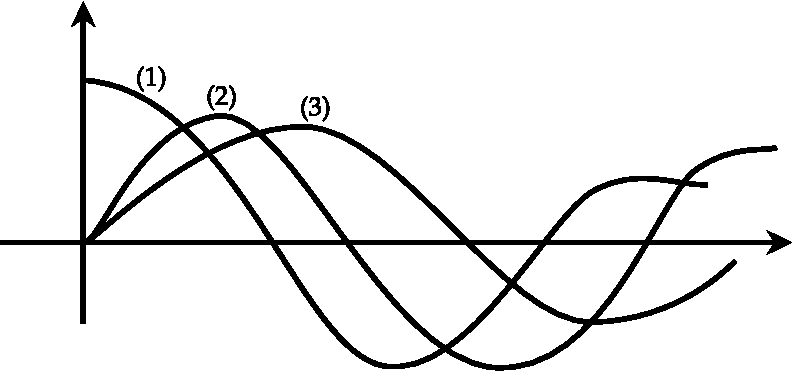
\includegraphics[height=3.5cm,width=6.5cm]{SF-01}
\end{figure}
 \begin{tasks}(2)
	\task[\textbf{a.}](1) $J_{0}$,
	(2) $J_{2}$, (3) $J_{1}$
	\task[\textbf{b.}]$(1) J_{0}$,
	(2) $J_{1}, \quad(3) J_{2}$
	\task[\textbf{c.}](1) $J_{2}$,
	(2) $J_{1}$,
	(3) $J_{0}$
	\task[\textbf{d.}] None of the above
\end{tasks}
\begin{answer}
	So the correct answer is \textbf{Option (b)}
\end{answer}
\item If the generating function of Legendre polynomial is $\frac{1}{\sqrt{1-6 t+t^{2}}}$, then coefficient of $t^{2}$ is
 \begin{tasks}(4)
	\task[\textbf{a.}] 11
	\task[\textbf{b.}]$-11$
	\task[\textbf{c.}]13
	\task[\textbf{d.}] $-13$
\end{tasks}
\begin{answer}
	\begin{align*}
	\intertext{The generating function for the polynomial solutions of the Legendre ODE is given by}
	g(x, t)&=\frac{1}{\sqrt{1-2 x t+t^{2}}}=\sum_{n=0}^{\infty} P_{n}(x) t^{n}\\
	\text{Thus }x&=3\text{ and }n=2.\\
	P_{2}(x)&=\frac{1}{2}\left(3 x^{2}-1\right) \Rightarrow P_{2}(3)=\frac{1}{2}\left(3 \times 3^{2}-1\right)=13
	\end{align*}
		So the correct answer is \textbf{Option (c)}
\end{answer}
\item Which of the following relation is true for Bessel's differential equation?
 \begin{tasks}(2)
	\task[\textbf{a.}]$J_{0}^{\prime}(x)=J_{1}(x)$
	\task[\textbf{b.}]$J_{0}^{\prime}(x)=-J_{2}(x)$
	\task[\textbf{c.}]$J_{0}^{\prime}(x)=J_{2}(x)$
	\task[\textbf{d.}] $J_{0}^{\prime}(x)=-J_{1}(x)$
\end{tasks}
\begin{answer}
	So the correct answer is \textbf{Option (d)}
\end{answer}
\item Given that $\sum_{n=0}^{\infty} H_{n}(x) \frac{t^{n}}{n !}=e^{-t^{2}+2 x x}$ the value of $H_{6}(0)$ is
 \begin{tasks}(4)
	\task[\textbf{a.}]$-120$
	\task[\textbf{b.}]$+120$
	\task[\textbf{c.}]12
	\task[\textbf{d.}]  $-12$
\end{tasks}
\begin{answer}
	\begin{align*}
	\sum_{n=0}^{\infty} I_{n}(x) \frac{t^{\prime \prime}}{n !}&=e^{-t^{2}+2 t x} \Rightarrow \sum_{n=0}^{\infty} H_{n}(0) \frac{t^{n}}{n !}=e^{-t^{2}}=1-t^{2}+\frac{t^{4}}{2 !}-\frac{t^{6}}{3 !}\\
	\Rightarrow \frac{H_{6}(0)}{6 !} t^{6}&=-\frac{1}{3 !} t^{6} \Rightarrow H_{6}(0)=-\frac{6 !}{3 !}=-120
	\end{align*}
	So the correct answer is \textbf{Option (a)}
\end{answer}
\item Given that $\sum_{n=0}^{\infty} H_{n}(x) \frac{t^{n}}{n !}=e^{-t^{2}+2 e x}$ the value of $H_{4}(0)$ is
 \begin{tasks}(4)
	\task[\textbf{a.}]12
	\task[\textbf{b.}] 6
	\task[\textbf{c.}]24
	\task[\textbf{d.}] $-6$
\end{tasks}
\begin{answer}
	\begin{align*}
	\sum_{n=0}^{\infty} H_{n}(x) \frac{t^{n}}{n !}&=e^{-t^{2}+2 t x} \Rightarrow \sum_{n=0}^{\infty} H_{n}(0) \frac{t^{n}}{n !}=e^{-t^{2}}=1-t^{2}+\frac{t^{4}}{2 !}-\frac{t^{6}}{3 !}\\
	\Rightarrow \frac{H_{4}(0)}{4 !} t^{4}&=\frac{t^{4}}{2 !} \Rightarrow H_{4}(0)=\frac{4 !}{2 !}=12
	\end{align*}
	So the correct answer is \textbf{Option (a)}
\end{answer}
\item If Hermite polynomial of order 2 is given by $H_{2}(x)=a x^{2}-2 ; a>0$, then the value of $a$ is
 \begin{tasks}(4)
	\task[\textbf{a.}]3
	\task[\textbf{b.}]4
	\task[\textbf{c.}]5
	\task[\textbf{d.}] 6
\end{tasks}
\begin{answer}
	\begin{align*}
	\intertext{Orthonormality condition,}
	\int_{-\infty}^{+\infty}\left[H_{n}(x)\right]^{2} e^{-x^{2}} d x&=2^{\prime \prime} n ! \sqrt{\pi}\\
	\text{For, }n&=2, \int_{-\infty}^{+\infty}\left(a x^{2}-2\right)^{2} e^{-x^{2}} d x=8 \sqrt{\pi}\\
\text{	Now}
	\int_{-\infty}^{+\infty}\left[H_{2}(x)\right]^{2} e^{-x^{2}} d x&=\int_{-\infty}^{+\infty}\left(a x^{2}-2\right)^{2} e^{-x^{2}} d x=\left\{a^{2} \times \frac{3}{4}+4-2 a\right\} \sqrt{\pi}
	\intertext{Thus, we have}
	\frac{3 a^{2}}{4}+4-2 a&=8 \Rightarrow 3 a^{2}-8 a-16=0 \Rightarrow 3 a^{2}-12 a+4 a-16=0\\
	\Rightarrow 3 a(a-4)+4(a-4)&=0 \Rightarrow(3 a+4)(a-4)=0\\
	\text{Thus, }a&=4
	\end{align*}
		So the correct answer is \textbf{Option (b)}
\end{answer}
\item The value of Legendre polynomial $p_{n}(x)$ for odd $n$ and $x=0$. i.e., $p_{n}(0)$ is
 \begin{tasks}(4)
	\task[\textbf{a.}]1
	\task[\textbf{b.}]0
	\task[\textbf{c.}]$-1$
	\task[\textbf{d.}]  $0.5$
\end{tasks}
\begin{answer}
	\begin{align*}
	\intertext{The generating function for Legendre polynomial is}
	\left(1-2 x t+t^{2}\right)^{-1 / 2}&=\sum_{n=0}^{\infty} p_{n}(x) t^{n}\\
	\text{Put, $x=0$, we get, }&\left(1+t^{2}\right)^{-1 / 2}=\sum p_{n}(\theta) t^{n}
	\end{align*}
		So the correct answer is \textbf{Option (b)}
\end{answer}
\item For the Legendre's polynomial $P_{n}(x)$, given below are two statements. Study these carefully and pick out the correct option.\\
Statement I: $\quad \int_{-1}^{1} x\left[P_{n}(x)\right]^{2} d x=0$\\
Statement I: $\lim _{n \rightarrow \infty}\left[\int_{-1}^{1} x P_{n}(x) P_{n+1}(x) d x\right]=0$
 \begin{tasks}(1)
	\task[\textbf{a.}]Only statement (I) is correct
	\task[\textbf{b.}]Only statement (II) is correct
	\task[\textbf{c.}]Both (I) and (II) are correct
	\task[\textbf{d.}]Neither (I) nor (II) is correet
\end{tasks}
\begin{answer}
	\begin{align*}
	\intertext{From recurrence relation we have}
	(n+1) P_{n+1}(x)&=(2 n+1) x p_{n}(x)-n p_{n-1}(x)\\
	x p_{n}(x)&=\frac{1}{(2 n+1)}\left\{(n+1) p_{n+1}(x)+n p_{n-1}(x)\right\}\\
	x\left[p_{n}(x)\right]^{2}&=\frac{1}{(2 n+1)}\left\{(n+1) p_{n}(x) p_{n+1}(x)+n p_{n}(x) p_{n-1}(x)\right\}\\
	\therefore \int_{-1}^{+1} x\left[p_{n}(x)\right]^{2} d x&=0\left\{\because \int_{-1}^{+1} p_{m}(x) p_{n}(x)=0\right.\text{ if }\left.m \neq n\right\}\\
	\therefore &\int_{-1}^{+1} x\left[p_{n}(x)\right]^{2} d x=0
	\intertext{From recurrence relation, we have}
	(n+1) p_{n+1}(x)&=(2 n+1) x p_{n}(x)-n p_{n-1}(x)\\
	(2 n+1) x p_{n}(x)&=(n+1) p_{n+1}(x)+n p_{n-1}(x)\\
	\int_{-1}^{+1}(2 n+1) x p_{n}(x) p_{n+1}(x) d x&=\int_{-1}^{+1}\left[(n+1)\left\{p_{n+1}(x)\right\}^{2}+n p_{n-1}(x) p_{n+1}(x)\right] d x\\
	=\int_{-1}^{+1}(n+1)\left\{p_{n+1}(x)\right\}^{2} d x+n \int_{-1}^{+1}& p_{n-1}(x) p_{n+1}(x) d x=(n+1) \frac{2}{2(n+1)+1}+0=\frac{2 n+2}{2 n+3}\\
	\therefore \int_{-1}^{+1} x p_{n}(x) p_{n+1}(x) d x&=\frac{2 n+2}{(2 n+1)(2 n+3)}\\
	\lim _{n \rightarrow \infty} \frac{n\left(2+\frac{2}{n}\right)}{n^{2}\left(2+\frac{1}{n}\right)\left(2+\frac{3}{n}\right)}&=\lim _{n \rightarrow \infty} \frac{\left(2+\frac{2}{n}\right)}{n\left(2+\frac{1}{n}\right)\left(2+\frac{3}{n}\right)}=0
	\end{align*}
		So the correct answer is \textbf{Option (c)}
\end{answer}
\item Which of the following statements is Incorrect about the Hermite polynomials $H_{n}(x)$ ?
 \begin{tasks}(1)
	\task[\textbf{a.}] The value of integral $\frac{1}{\sqrt{\pi}} \int_{-\infty}^{\infty} e^{-x^{2}}\left[H_{4}(x)\right]^{2} d x$ is 384
	\task[\textbf{b.}] Hermite polynomial of order $3, H_{3}(x)$, satisfies the differential equation $y^{\prime \prime}-2 x y^{\prime}+6 y=0$
	\task[\textbf{c.}] The value of $\mathrm{H}_{4}(\mathrm{l})$ is $-20$
	\task[\textbf{d.}] $H_{n}(x)=\frac{H_{n+1}(x)+2 n H_{n-1}(x)}{x}$
\end{tasks}
\begin{answer}
	\begin{align*}
	\intertext{When integrated with respect to weight function $e^{-x^{2}}$, the Hermite polynomials satisfy}
	\int_{-\infty}^{\infty} e^{-x^{2}} H_{n}(x) H_{m}(x) d x&= \begin{cases}0, & n \neq m \\ \sqrt{\pi} 2^{n} n !, & n=m\end{cases}
	\intertext{In our case $n=m=4$, hence}
	\frac{1}{\sqrt{\pi}} \int_{-\infty}^{\infty} e^{-x^{2}}\left[H_{4}(x)\right]^{2} d x&=\frac{\sqrt{\pi} 2^{4}(4 !)}{\sqrt{\pi}}=384
	\intertext{Hermite polynomial of order $n$, satisfies the differential equation}
	y^{\prime \prime}-2 x y^{\prime}+2 n y=0\\
\text{	when }n=3, y^{\prime \prime}-2 x y^{\prime}+6 y=0\\
	\text{We have }H_{4}(x)&=16 x^{4}-48 x^{2}+12\\
	\text{Therefore, }H_{4}(1)&=-48+28=-20
	\intertext{The recursion relation for Hermite polynomials is}
	H_{n+1}(x)&=2 x H_{n}(x)-2 n H_{n-1}(x) \Rightarrow H_{n}(x)=\frac{H_{n+1}(x)+2 n H_{n-1}(x)}{2 x}
	\end{align*}
		So the correct answer is \textbf{Option (d)}
\end{answer}
\item If $P_{n}(x)$ denotes the Legendre polynomials of order $n$, then which of the following statements is incorrect?
 \begin{tasks}(1)
	\task[\textbf{a.}]$P_{n}(x)=\frac{1}{2^{n} n !} \frac{d^{n}}{d x^{n}}\left[\left(x^{2}-1\right)^{n}\right]$ where $n=0,1,2 \ldots$
	\task[\textbf{b.}]The Legendre polynomials satisfy the differential equation\\$
	\left(1-x^{2}\right) \frac{d^{2} y}{d x^{2}}-2 x \frac{d y}{d x}+n(n+1) y=0
	$
	\task[\textbf{c.}] For each value of $n$ the Legendre polynomials satisfy the relation $P_{n}(1)=1$.
	\task[\textbf{d.}] The value of integral $\int_{-1}^{1}\left[P_{4}(x)\right]^{2} d x$ is $\frac{2}{7}$.
\end{tasks}
\begin{answer}
	\begin{align*}
	\intertext{Option (a) is the correct definition of Legendre polynomial. Legendre polynoimials satisfy the differential equation given in option (b). For each value of $n$ Legendre polynomials satisfy $P_{n}(1)=1$.}
	\text{Since, }\int_{-1}^{1}\left[P_{n}(x)\right]^{2} d x&=\frac{2}{2 n+1}\\
	\text{Hence, }\int_{-1}^{1}\left[P_{4}(x)\right]^{2} d x&=\frac{2}{2 \cdot 4+1}=\frac{2}{9}\\
	\text{Hence option }&(d)\text{ is incorrect.}
	\end{align*}
		So the correct answer is \textbf{Option (d)}
\end{answer}
\end{enumerate}
%\input{chapter/Practice set Solutions}
%\chapter{Practice set Solutions Differential Equations}
\begin{abox}
	Problem Set -1
\end{abox}
\begin{enumerate}[label=\color{ocre}\textbf{\arabic*.}]	
	\item Let $x_{1}(t)$ and $x_{2}(t)$ be two linearly independent solutions of the differential equation $\frac{d^{2} x}{d t^{2}}+2 \frac{d x}{d t}+f(t) x=0$ and let $w(t)=x_{1}(t) \frac{d x_{2}(t)}{d t}-x_{2}(t) \frac{d x_{1}(t)}{d t} .$ If $w(0)=1$, then $w(1)$ is given by
	{\exyear{ NET/JRF(DEC-2011)}}
			\begin{tasks}(4)
			\task[\textbf{A.}] 1
			\task[\textbf{B.}] $e^{2}$
			\task[\textbf{C.}]  $1 / e$
			\task[\textbf{D.}] $1 / e^{2}$
		\end{tasks}
			\begin{answer}
			\begin{align*}
			\intertext{$W(t)$ is Wronskian of D.E.}
			W&=e^{-\int \mathrm{Pdt}}=e^{-2 t} \Rightarrow W(1)\\&=e^{-2}\text{ since }P=2
			\end{align*}
			So the correct answer is \textbf{Option (D)}
		\end{answer}
\item Let $y(x)$ be a continuous real function in the range 0 and $2 \pi$, satisfying the inhomogeneous differential equation: $\sin x \frac{d^{2} y}{d x^{2}}+\cos x \frac{d y}{d x}=\delta\left(x-\frac{\pi}{2}\right)$ The value of $d y l d x$ at the point $x=\pi / 2$
{\exyear{NET/JRF (JUNE-2012)}}
\begin{tasks}(2)
	\task[\textbf{A.}] Is continuous
	\task[\textbf{B.}] Has a discontinuity of 3
	\task[\textbf{C.}] Has a discontinuity of $1 / 3$
	\task[\textbf{D.}] Has a discontinuity of 1
\end{tasks}
\begin{answer}
	\begin{align*}
	\text{After dividing by }\sin x, \frac{d^{2} y}{d x^{2}}+\cot x \frac{d y}{d x}&=\operatorname{cosec} x \cdot \delta\left(x-\frac{\pi}{2}\right)\\
	\text{Integrating both sides, }\frac{d y}{d x}+\int \cot x\left(\frac{d y}{d x}\right) d x&=\int \operatorname{cosec} x \delta\left(x-\frac{\pi}{2}\right) d x\\
	\frac{d y}{d x}+\cot x \cdot y-\int \operatorname{cosec}^{2} x \cdot y d x&=1\\
	\text{Using Dirac delta property: }\int f(x) \delta\left(x-x_{0}\right)&=f\left(x_{0}\right)\text{ (it lies with the limit).}\\
	\frac{d y}{d x}+y \cdot \frac{\cos x}{\sin x}-\int y \operatorname{cosec}^{2} x d x&=1,\text{ at }x=\pi ; \sin x=0 .\text{ So this is point of discontinuity.}
	\end{align*}
	So the correct answer is \textbf{Option (D)}
\end{answer}
\item The solution of the partial differential equation
$$
\frac{\partial^{2}}{\partial t^{2}} u(x, t)-\frac{\partial^{2}}{\partial x^{2}} u(x, t)=0
$$
satisfying the boundary conditions $u(0, t)=0=u(L, t)$ and initial conditions $u(x, 0)=\sin (\pi x / L)$ and $\left.\frac{\partial}{\partial t} u(x, t)\right|_{t=0}=\sin (2 \pi x / L)$ is
{\exyear{NET/JRF(JUNE-2013)}}
	\begin{tasks}(1)
		\task[\textbf{A.}] $\sin (\pi x / L) \cos (\pi t / L)+\frac{L}{2 \pi} \sin (2 \pi x / L) \cos (2 \pi t / L)$
		\task[\textbf{B.}] $2 \sin (\pi x / L) \cos (\pi t / L)-\sin (\pi x / L) \cos (2 \pi t / L)$
		\task[\textbf{C.}] $\sin (\pi x / L) \cos (2 \pi t / L)+\frac{L}{\pi} \sin (2 \pi x / L) \sin (\pi t / L)$
		\task[\textbf{D.}] $\sin (\pi x / L) \cos (\pi t / L)+\frac{L}{2 \pi} \sin (2 \pi x / L) \sin (2 \pi t / L)$
	\end{tasks}
	\begin{answer}
		\begin{align*}
		\frac{\partial^{2} u}{\partial t^{2}}-\frac{\partial^{2} u}{\partial x^{2}}&=0, u(x, 0)=\sin \frac{\pi x}{L}\text{ and }\left.\frac{\partial u}{\partial t}\right|_{t=0}=\sin \frac{2 \pi x}{L}\\
		\text{This is a wave equation}\\
		\text{So solution is given by }u(x, t)&=\sum_{n}\left(A_{n} \cos \frac{a n \pi t}{L}+B_{n} \sin \frac{a n \pi t}{L}\right) \sin \left(\frac{n \pi x}{L}\right)\\
		\text{with }A_{n}&=\frac{2}{L} \int_{0}^{L} f(x) \sin \frac{n \pi x}{L} d x, \\ B_{n}&=\frac{2}{a n \pi} \int_{0}^{L} g(x) \sin \frac{n \pi x}{L} d x\\
		\text{Comparing }a^{2} \frac{\partial^{2} u}{\partial t^{2}}&=\frac{\partial^{2} u}{\partial x^{2}},\text{ We have }a=1\text{ and }f(x)\\&=\sin \frac{\pi x}{L}, g(x)=\sin \frac{2 \pi x}{L}\\
		A_{n}&=\frac{2}{L} \int_{0}^{L} \sin \frac{\pi x}{L} \sin \frac{n \pi x}{L} d x \Rightarrow \frac{2}{L} \int_{0}^{L} \sin ^{2} \frac{\pi x}{L} d x\\&=\frac{2}{L} \int_{0}^{L}\left(\frac{1-\cos \frac{2 \pi x}{L}}{2}\right) d x=\frac{2}{L} \cdot \frac{L}{2}=1 (\text{let }\left.n=1\right)\\
		\text{Putting }n&=2, B_{n}=\frac{2}{a n \pi} \int_{0}^{L} \sin \frac{2 \pi x}{L} \cdot \sin \frac{n \pi x}{L} d x\\
		\Rightarrow \frac{2}{2 \pi} \int_{0}^{L} \sin ^{2} \frac{2 \pi x}{L} d x&=\frac{2}{2 \pi} \int_{0}^{L}\left(\frac{1-\cos \frac{4 \pi x}{L}}{2}\right) d x=\frac{2}{2 \pi} \cdot \frac{L}{2}=\frac{L}{2 \pi}
		\end{align*}
		So the correct answer is \textbf{Option (D)}
	\end{answer}
	\item The solution of the differential equation
	$$
	\frac{d x}{d t}=x^{2}
	$$
	with the initial condition $x(0)=1$ will blow up as $t$ tends to
	{\exyear{NET/JRF(JUNE-2013)}}
	\begin{tasks}(4)
		\task[\textbf{A.}] 1
		\task[\textbf{B.}] 2
		\task[\textbf{C.}] $\frac{1}{2}$
		\task[\textbf{D.}] $\infty$
	\end{tasks}
	\begin{answer}
		\begin{align*}
		\frac{d x}{d t}&=x^{2} \Rightarrow \int \frac{d x}{x^{2}}=\int d t \Rightarrow \frac{x^{-2+1}}{-2+1}\\&=t+C \Rightarrow \frac{-1}{x}=t+C\\
		\Rightarrow x(0)&=1 \Rightarrow \frac{-1}{1}=0+C \Rightarrow C=-1 \Rightarrow \frac{-1}{x}\\&=t-1 \Rightarrow x=\frac{1}{1-t}\text{ as }t \rightarrow 1, x\text{ blows up}
		\end{align*}
		So the correct answer is \textbf{Option (A)}
	\end{answer}
	\item Consider the differential equation
	$$
	\frac{d^{2} x}{d t^{2}}+2 \frac{d x}{d t}+x=0
	$$
	with the initial conditions $x(0)=0$ and $\dot{x}(0)=1$. The solution $x(t)$ attains its maximum value when $t$ is
	{\exyear{NET/JRF(JUNE-2014)}}
	\begin{tasks}(4)
		\task[\textbf{A.}] $1 / 2$
		\task[\textbf{B.}] 1
		\task[\textbf{C.}] 2
		\task[\textbf{D.}] $\infty$
	\end{tasks}
	\begin{answer}
		\begin{align*}
		\frac{d^{2} x}{d t^{2}}+2 \frac{d x}{d t}+x&=0 \Rightarrow m^{2}+2 m+1\\&=0 \Rightarrow(m+1)^{2}=0 \Rightarrow m=-1,-1\\
		\Rightarrow x&=\left(c_{1}+c_{2} t\right) e^{-t},\text{ since }x(0)\\&=0 \Rightarrow 0=c_{1} \Rightarrow x=c_{2} t e^{-t}\\
		\Rightarrow \dot{x}&=c_{2}\left[-t e^{-t}+e^{-t}\right]\\
		\text{Since }\dot{x}(0)&=1 \Rightarrow 1=c_{2} \Rightarrow x=t e^{-t}\\
		\text{For maxima or minima }\dot{x}&=0 \Rightarrow \dot{x}=-t e^{-t}+e^{-t}=0 \Rightarrow \dot{x}=e^{-t}(1-t)\\
		\Rightarrow e^{-t}&=0,1-t=0 \Rightarrow t=\infty, t=1\\
		\ddot{x}&=e^{-t}(-1)+(1-t) e^{-t}(-1)\\&=-e^{-t}+(t-1) e^{-t} \Rightarrow \ddot{x}(1)\\&=-e^{-1}+0 e^{-t}<0
		\end{align*}
		So the correct answer is \textbf{Option (B)}
	\end{answer}
	\item Consider the differential equation $\frac{d^{2} x}{d t^{2}}-3 \frac{d x}{d t}+2 x=0$. If $x=0$ at $t=0$ and $x=1$ at $t=1$, the value of $x$ at $t=2$ is
	{\exyear{NET/JRF(JUNE-2015)}}
	\begin{tasks}(4)
		\task[\textbf{A.}] $e^{2}+1$
		\task[\textbf{B.}] $e^{2}+e$
		\task[\textbf{C.}] $e+2$
		\task[\textbf{D.}] $2 e$
	\end{tasks}
	\begin{answer}
		\begin{align*}
		D^{2}-3 D+2&=0\\
		(D-1)(D-2)&=0 \Rightarrow D=1,2 \Rightarrow x=c_{1} e^{2 t}+c_{2} e^{t}\\
		\text{using boundary condition }x&=0, t=0 \Rightarrow c_{1}=-C_{2}\\
		\text{again using boundary condition }x&=1, t=1\\
		c_{2}&=\frac{1}{e-e^{2}}, c_{1}=\frac{1}{e^{2}-e} \Rightarrow x\\&=\frac{e^{2 t}}{e^{2}-e}+\frac{1}{e-e^{2}} e^{t}\\
		\text{again using }t&=2\text{ then }x=e^{2}+e
		\end{align*}
		So the correct answer is \textbf{Option (B)}
	\end{answer}
	\item  If $y=\frac{1}{\tanh (x)}$, then $x$ is
	{\exyear{NET/JRF(DEC-2015)}}
	\begin{tasks}(4)
		\task[\textbf{A.}] $\ln \left(\frac{y+1}{y-1}\right)$
		\task[\textbf{B.}] $\ln \left(\frac{y-1}{y+1}\right)$
		\task[\textbf{C.}]  $\ln \sqrt{\frac{y-1}{y+1}}$
		\task[\textbf{D.}]  $\ln \sqrt{\frac{y+1}{y-1}}$
	\end{tasks}
	\begin{answer}
		\begin{align*}
		y&=\frac{1}{\tanh x}\\
		y&=\frac{e^{x}+e^{-x}}{e^{x}-e^{-x}}=\frac{e^{2 x}+1}{e^{2 x}-1}\\
		y e^{2 x}-y&=e^{2 x}+1 \Rightarrow y e^{2 x}-e^{2 x}\\&=1+y \Rightarrow e^{2 x}(y-1)=(1+y)\\
		2 x&=\ln \left(\frac{y+1}{y-1}\right) \Rightarrow x=\frac{1}{2} \ln \left(\frac{y+1}{y-1}\right)\\&=\ln \left(\frac{y+1}{y-1}\right)^{\frac{1}{2}}
		\end{align*}
		So the correct answer is \textbf{Option (D)}
	\end{answer}
	\item The solution of the differential equation $\frac{d x}{d t}=2 \sqrt{1-x^{2}}$, with initial condition $x=0$ at $t=0$ is
	{\exyear{NET/JRF(DEC-2015)}}
	\begin{tasks}(2)
		\task[\textbf{A.}] $x=\left\{\begin{array}{ll}\sin 2 t, & 0 \leq t<\frac{\pi}{4} \\ \sinh 2 t, & t \geq \frac{\pi}{4}\end{array}\right.$
		\task[\textbf{B.}] $x=\left\{\begin{array}{cc}\sin 2 t, & 0 \leq t<\frac{\pi}{2} \\ 1, & t \geq \frac{\pi}{2}\end{array}\right.$
		\task[\textbf{C.}] $x=\left\{\begin{array}{cc}\sin 2 t, & 0 \leq t<\frac{\pi}{4} \\ 1, & t \geq \frac{\pi}{4}\end{array}\right.$
		\task[\textbf{D.}] $x=1-\cos 2 t, \quad t \geq 0$
	\end{tasks}
	\begin{answer}
		\begin{align*}
		\frac{d x}{d t}&=2 \sqrt{1-x^{2}}, \frac{d x}{\sqrt{1-x^{2}}}\\&=2 d t, \sin ^{-1} x=2 t+c, x=0, t=0 \\\text{ so, }c&=0 \Rightarrow x=\sin 2 t\\
		&\text{	$x$ should not be greater than 1 at $x=1$}\\
		1&=\sin 2 t, \quad \sin \frac{\pi}{2}=\sin 2 t, t=\frac{\pi}{4}\\
		\text{	So, }\quad x&=\left\{\begin{array}{ll}\sin 2 t, & 0 \leq t<\frac{\pi}{4} \\ 1, & t \geq \frac{\pi}{4}\end{array}\right.
		\end{align*}
		So the correct answer is \textbf{Option (C)}
	\end{answer}
	\item   The function $y(x)$ satisfies the differential equation $x \frac{d y}{d x}+2 y=\frac{\cos \pi x}{x}$. If $y(1)=1$, the value of $y(2)$ is
	{\exyear{NET/JRF(JUNE-2017)}}
	\begin{tasks}(4)
		\task[\textbf{A.}] $\pi$
		\task[\textbf{B.}] 1
		\task[\textbf{C.}] $1 / 2$
		\task[\textbf{D.}] $1 / 4$
	\end{tasks}
	\begin{answer}
		\begin{align*}
		\intertext{The given differential equation can be written as}
		\frac{d y}{d x}+\frac{2}{x} y&=\frac{\cos \pi x}{x^{2}}
		\intertext{This is a linear differential equation with Integrating factor $=e^{\int_{x}^{2} d x}=x^{2}$}
		\text{Hence }y . x^{2}&=\int x^{2} \cdot \frac{\cos \pi x}{x^{2}} d x+c \Rightarrow y\\&=\frac{\sin \pi x}{\pi x^{2}}+\frac{c}{x^{2}}\\
		\text{when }x&=1, y=1\text{ hence }c=1 \Rightarrow y\\&=\frac{\sin \pi x}{\pi x^{2}}+\frac{1}{x^{2}}\\
		\text{hence, when }x&=2, y=\frac{1}{4}
		\end{align*}
		So the correct answer is \textbf{Option (D)}
	\end{answer}
	\item   Consider the differential equation $\frac{d y}{d t}+a y=e^{-b t}$ with the initial condition $y(0)=0$. Then the Laplace transform $Y(s)$ of the solution $y(t)$ is
	{\exyear{NET/JRF(DEC-2017)}}
	\begin{tasks}(4)
		\task[\textbf{A.}] $\frac{1}{(s+a)(s+b)}$
		\task[\textbf{B.}] $\frac{1}{b(s+a)}$
		\task[\textbf{C.}] $\frac{1}{a(s+b)}$
		\task[\textbf{D.}] $\frac{e^{-a}-e^{-b}}{b-a}$
	\end{tasks}
	\begin{answer}
		\begin{align*}
		\text{Given }\frac{d y}{d t}+a y&=e^{-b t}
		\intertext{Taking Laplace transform of both sides}
		\text{	We obtain}\\
		L\left\{\frac{d y}{d t}\right\}+a L\{y(t)\}&=L\left\{e^{-b t}\right\} \Rightarrow s Y(s)-y(0)+a Y(s)=\frac{1}{s+b}\\
		\text{Since, }	y(0)&=0,\text{ we obtain}\\
		(s+a) Y(s)&=\frac{1}{s+b} \Rightarrow Y(s)=\frac{1}{(s+a)(s+b)}
		\end{align*}
		So the correct answer is \textbf{Option (A)}
	\end{answer}
	\item The number of linearly independent power series solutions, around $x=0$, of the second order linear differential equation $x \frac{d^{2} y}{d x^{2}}+\frac{d y}{d x}+x y=0$, is
	{\exyear{NET/JRF(DEC-2017)}}
	\begin{tasks}(1)
		\task[\textbf{A.}] 0 (this equation does not have a power series solution)
		\task[\textbf{B.}] 1
		\task[\textbf{C.}] 2
		\task[\textbf{D.}] 3
	\end{tasks}
	\begin{answer}
		So the correct answer is \textbf{Option (B)}
	\end{answer}
	\item The differential equation $\frac{d y(x)}{d x}=\alpha x^{2}$, with the initial condition $y(0)=0$, is solved using Euler's method. If $y_{E}(x)$ is the exact solution and $y_{N}(x)$ the numerical solution obtained using $n$ steps of equal length, then the relative error $\left|\frac{\left(y_{N}(x)-y_{E}(x)\right)}{y_{E}(x)}\right|$ is proportional to
	{\exyear{NET/JRF(DEC-2017)}}
	\begin{tasks}(4)
		\task[\textbf{A.}] $\frac{1}{n^{2}}$
		\task[\textbf{B.}] $\frac{1}{n^{3}}$
		\task[\textbf{C.}] $\frac{1}{n^{4}}$
		\task[\textbf{D.}] $\frac{1}{n}$
	\end{tasks}
	\begin{answer}
		\begin{align*}
		\frac{d y}{d x}&=\alpha x^{2}, y(0)=0\\
		y_{E}&=\frac{\alpha x^{3}}{3},\text{ but }x=n \hbar\\
		\text{Exact solution, }y_{E}&=\frac{\alpha n^{3} h^{3}}{3}\\
		\text{Numerically, }f(x, y)&=\alpha x^{2}\\
		\text{Euler's method, }y_{i}&=y_{i-1}+h f\left(x_{i-1}, y_{i-1}\right)\\
		y_{1}&=0, y_{2}=\alpha h^{3} \quad y_{3}=5 \alpha h^{3}\\
		y_{n}&=\frac{(n-1) n(2 n-1)}{6} \alpha h^{3}
		\intertext{Since, $0,5,14,30, \ldots$ different from square terms}
		\intertext{At, $x_{0}=0 \quad x_{1}=x_{0}+h=h \quad x_{2}=x_{0}+2 h=2 h \quad x_{3}=x_{0}+3 h=3 h$}
		x_{n-1}&=x_{0}+(n-1) h=(n-1) h .\text{ Now, }x_{n}=n h\\
		f\left(x_{0}, y_{0}\right)
		&=0, f\left(x_{1}, y_{1}\right)=\alpha h^{2}, f\left(x_{2}, y_{2}\right)=4 \alpha h^{2}\\
		f\left(x_{n-1}, y_{n-1}\right)&=\alpha(n-1)^{2} h^{2}\\
		\left|\frac{\left(y_{N}-y_{E}\right)}{y_{E}}\right|&=\left|\frac{\frac{(n-1) n(2 n-1) \alpha h^{3}}{6}-\frac{\alpha n^{3} h^{3}}{3}}{\frac{\alpha n^{3} h^{3}}{3}}\right|\\
		\text{By solving, }&\left|\frac{y_{N}-y_{E}}{y_{E}}\right| \propto \frac{1}{n}
		\end{align*}
		So the correct answer is \textbf{Option (D)}
	\end{answer}
	\item  Consider the following ordinary differential equation
	$$
	\frac{d^{2} x}{d t^{2}}+\frac{1}{x}\left(\frac{d x}{d t}\right)^{2}-\frac{d x}{d t}=0
	$$
	with the boundary conditions $x(t=0)=0$ and $x(t=1)=1 .$ The value of $x(t)$ at $t=2$ is
	{\exyear{NET/JRF(JUNE-2018)}}
	\begin{tasks}(4)
		\task[\textbf{A.}] $\sqrt{e-1}$
		\task[\textbf{B.}] $\sqrt{e^{2}+1}$
		\task[\textbf{C.}]  $\sqrt{e+1}$
		\task[\textbf{D.}] $\sqrt{e^{2}-1}$
	\end{tasks}
	\begin{answer}
		\begin{align*}
		\intertext{The given equation can be written as}
		\frac{1}{x} \frac{d}{d t}\left(x \frac{d x}{d t}\right)-\frac{d x}{d t}&=0 \Rightarrow \frac{d}{d t}\left(x \frac{d x}{d t}\right)-x \frac{d x}{d t}=0\\
		\text{putting }y&=x \frac{d x}{d t}\text{ gives}\\
		\frac{d y}{d t}-y&=0 \Rightarrow \ln y=t+\ln c_{1} \Rightarrow y=c_{1} e^{t}\\
		\intertext{Since $x \frac{d x}{d t}=c_{1} e^{t}$ hence by integrating}
		\frac{x^{2}}{2}&=c_{1} e^{t}+c_{2}\hspace{2cm}\text{(i)}
		\intertext{Using boundary conditions we obtain}
		c_{1}+c_{2}&=0\text{ and }c_{1} e+c_{2}=\frac{1}{2}
		\intertext{Solving these equations we obtain $c_{1}=\frac{1}{2(e-1)}$ and $c_{2}=-\frac{1}{2(e-1)}$}
		\text{Thus, }\frac{x^{2}}{2}&=\frac{1}{2(e-1)} e^{t}-\frac{1}{2(e-1)}\\
		\text{When }t&=2,\text{ we obtain, }\quad x^{2}=\frac{e^{2}}{(e-1)}-\frac{1}{(e-1)}\\&=\frac{\left(e^{2}-1\right)}{(e-1)}=e+1\\
		\text{Therefore}x(2)&=\sqrt{e+1}
		\end{align*}
		So the correct answer is \textbf{Option (C)}
	\end{answer}
	\item  In terms of arbitrary constants $A$ and $B$, the general solution to the differential equation $x^{2} \frac{d^{2} y}{d x^{2}}+5 x \frac{d y}{d x}+3 y=0$ is
	{\exyear{NET/JRF(DEC-2018)}}
	\begin{tasks}(4)
		\task[\textbf{A.}]  $y=\frac{A}{x}+B x^{3}$
		\task[\textbf{B.}] $y=A x+\frac{B}{x^{3}}$
		\task[\textbf{C.}] $y=A x+B x^{3}$
		\task[\textbf{D.}] $y=\frac{A}{x}+\frac{B}{x^{3}}$
	\end{tasks}
	\begin{answer}
		\begin{align*}
		\intertext{
			The given equation is Euler-Cauchy differential equation. The characteristic equation of}
		x^{2} \frac{d^{2} y}{d x^{2}}+5 x \frac{d y}{d x}+6 y&=0\\
		\text{is ,}m^{2}+4 m+6&=0 \Rightarrow m=-3 or m=-1\\
		\text{Thus, }y_{1}&=x^{-1}=\frac{1}{x}\text{ and }y_{2}=x^{2}=\frac{1}{x^{3}}
		\intertext{Therefore the general solution is}
		y&=\frac{A}{x}+\frac{B}{x^{3}}
		\end{align*}
		So the correct answer is \textbf{Option (D)}
	\end{answer}
	\item The solution of the differential equation $x \frac{d y}{d x}+(1+x) y=e^{-x}$ with the boundary condition $y(x=1)=0$, is
	{\exyear{NET/JRF(JUNE-2019)}}
	\begin{tasks}(4)
		\task[\textbf{A.}] $\frac{(x-1)}{x} e^{-x}$
		\task[\textbf{B.}] $\frac{(x-1)}{x^{2}} e^{-x}$
		\task[\textbf{C.}] $\frac{(1-x)}{x^{2}} e^{-x}$
		\task[\textbf{D.}] $(x-1)^{2} e^{-x}$
	\end{tasks}
	\begin{answer}
		\begin{align*}
		x \frac{d y}{d x}+(1+x) y&=e^{-x} \Rightarrow \frac{d y}{d x}+\frac{(1+x)}{x} y=\frac{e^{-x}}{x}\\
		\text{Let }p&=\frac{1+x}{x}\\
		I.F &=e^{\int p d x}=e^{\int\left(1+\frac{1}{x}\right) d x}=e^{x} \cdot e^{\ln x}=x e^{x}\\
		y \cdot x \cdot e^{x}&=\int \frac{e^{-x}}{x} \cdot x e^{x} d x+C \Rightarrow y \cdot x \cdot e^{x}=x+C\\
		y&=0\text{ at }x=1 \quad \Rightarrow C=-1 \quad \Rightarrow y \cdot x \cdot e^{x}\\&=x-1 \Rightarrow y=\left[\frac{x-1}{x}\right] e^{-x}
		\end{align*}
		So the correct answer is \textbf{Option (A)}
	\end{answer}
	\item The solution of the differential equation $\left(\frac{d y}{d x}\right)^{2}-\frac{d^{2} y}{d x^{2}}=e^{y}$, with the boundary conditions $y(0)=0$ and $y^{\prime}(0)=-1$, is
	{\exyear{NET/JRF(JUNE-2020)}}
	\begin{tasks}(4)
		\task[\textbf{A.}] $-\ln \left(\frac{x^{2}}{2}+x+1\right)$
		\task[\textbf{B.}] $-x \ln (e+x)$
		\task[\textbf{C.}] $-x e^{-x^{2}}$
		\task[\textbf{D.}]  $-x(x+1) e^{-x}$
	\end{tasks}
	\begin{answer}
		\begin{align*}
		\left(\frac{d y}{d x}\right)^{2}-\frac{d^{2} y}{d x^{2}}&=e^{y}\text{ put }y=\ln p\\
		\frac{d y}{d x}&=\frac{1}{p} \frac{d p}{d x} \Rightarrow \frac{d^{2} y}{d x^{2}}=\frac{d}{d x}\left(\frac{1}{p} \frac{d p}{d x}\right)\\&=\frac{1}{p} \frac{d^{2} p}{d x^{2}}-\frac{1}{p^{2}}\left(\frac{d p}{d x}\right)^{2}\\
		\text{Thus }&\left(\frac{1}{p} \frac{d p}{d x}\right)^{2}-\frac{1}{p} \frac{d^{2} p}{d x^{2}}+\frac{1}{p^{2}}\left(\frac{d p}{d x}\right)^{2}=p\\
		\frac{2}{p^{2}}\left(\frac{d p}{d x}\right)^{2}-\frac{1}{p} \frac{d^{2} p}{d x^{2}}&=p \Rightarrow \frac{2}{p^{3}}\left(\frac{d p}{d x}\right)^{2}-\frac{1}{p^{2}} \frac{d^{2} p}{d x^{2}}\\&=1 \Rightarrow \frac{1}{p^{2}} \frac{d^{2} p}{d x^{2}}-\frac{2}{p^{3}}\left(\frac{d p}{d x}\right)^{2}=-1\\
		&\Rightarrow \frac{d}{d x}\left(\frac{1}{p^{2}} \frac{d p}{d x}\right)=-1\\
		\text{Let }\frac{1}{p^{2}} \frac{d p}{d x}&=z \Rightarrow \frac{d z}{d x}=-1 \Rightarrow z=-x+c\\
		\text{Thus }\frac{1}{p^{2}} \frac{d p}{d x}&=-x+c \Rightarrow \int \frac{d p}{p^{2}}=\int(-x+c) d x\\
		-\frac{1}{p}&=-\frac{x^{2}}{2}+c x+d \Rightarrow p=\frac{1}{\frac{x^{2}}{2}-c x-d}\\
		y&=\ln p=\ln \left(\frac{1}{\frac{x^{2}}{2}-c x-d}\right)=\ln \left(\frac{x^{2}}{2}-c x-d\right)\\
		y(0)&=0 \Rightarrow y(0)=-\ln (-d) \Rightarrow d=-1\\
		y&=-\ln \left(\frac{x^{2}}{2}-c x+1\right)\\
		y^{\prime}(x)&=-\frac{1}{\left(\frac{x^{2}}{2}-c x+1\right)}(x-c), \quad y^{\prime}(0)\\&=-1 \Rightarrow-\frac{(-c)}{1}=c=-1, \quad y=-\ln \left(\frac{x^{2}}{2}+x+1\right)
		\end{align*}
		So the correct answer is \textbf{Option (A)}
	\end{answer}
\end{enumerate}
 \colorlet{ocre1}{ocre!70!}
\colorlet{ocrel}{ocre!30!}
\setlength\arrayrulewidth{1pt}
\begin{table}[H]
	\centering
	\arrayrulecolor{ocre}
	\begin{tabular}{|p{1.5cm}|p{1.5cm}||p{1.5cm}|p{1.5cm}|}
		\hline
		\multicolumn{4}{|c|}{\textbf{Answer key}}\\\hline\hline
		\rowcolor{ocrel}Q.No.&Answer&Q.No.&Answer\\\hline
		1&\textbf{D} &2&\textbf{D}\\\hline 
		3&\textbf{D} &4&\textbf{A} \\\hline
		5&\textbf{B} &6&\textbf{B} \\\hline
		7&\textbf{D}&8&\textbf{C}\\\hline
		9&\textbf{D}&10&\textbf{A}\\\hline
		11&\textbf{B} &12&\textbf{D}\\\hline
		13&\textbf{C}&14&\textbf{D}\\\hline
		15&\textbf{A}&16&\textbf{A} \\\hline
		
	\end{tabular}
\end{table}
\newpage
\begin{abox}
	Problem Set -2
\end{abox}
\begin{enumerate}[label=\color{ocre}\textbf{\arabic*.}]
	\item  The solution of the differential equation for $y(t): \frac{d^{2} y}{d t^{2}}-y=2 \cosh (t)$, subject to the initial conditions $y(0)=0$ and $\left.\frac{d y}{d t}\right|_{t=0}=0$, is
	{\exyear{GATE 2010}}
	\begin{tasks}(2)
		\task[\textbf{A.}] $\frac{1}{2} \cosh (t)+t \sinh (t)$
		\task[\textbf{B.}] $-\sinh (t)+t \cosh (t)$
		\task[\textbf{C.}] $t \cosh (t)$
		\task[\textbf{D.}] $t \sinh (t)$
	\end{tasks}
	\begin{answer}
		\begin{align}
		\text{	For C.F } \left(D^{2}-1\right) y&=0 \Rightarrow m=\pm 1 \Rightarrow C . F .\notag\\&=C_{1} e^{t}+C_{2} e^{-t}\notag\\
		P.I. &=\frac{1}{D^{2}-1}(2 \cosh t)=\frac{1}{D^{2}-1} 2\left(\frac{e^{t}+e^{-t}}{2}\right)\notag\\&=\frac{1}{D^{2}-1}\left(e^{t}\right)+\frac{1}{D^{2}-1}\left(e^{-t}\right)\notag\\&=\frac{t}{2} e^{t}+\frac{t}{2}\left(-e^{-t}\right)\notag\\
		\Rightarrow y&=C_{1} e^{t}+C_{2} e^{-t}+\frac{t}{2} e^{t}-\frac{t}{2} e^{-t}\notag\\
		\text{As, }y(0)&=0 \Rightarrow C_{1}+C_{2}=0\label{math01}\\
		\frac{d y}{d t}&=C_{1} e^{t}-C_{2} e^{-t}+\frac{t}{2} e^{t}+\frac{1}{2} e^{t}+\frac{t}{2} e^{-t}-\frac{1}{2} e^{-t}\notag\\
		\text{Also, }\left.\frac{d y}{d t}\right|_{t=0}&=0 \Rightarrow C_{1}-C_{2}+0+\frac{1}{2}+0-\frac{1}{2}=0 \Rightarrow C_{1}-C_{2}=0\label{math02}\\
		\text{From equation (\ref{math01}) and (\ref{math02}),}\notag\\
		C_{1}&=0, C_{2}=0\notag\\
		\text{Thus }y&=\frac{t}{2} e^{t}-\frac{t}{2} e^{-t} \Rightarrow y=t \sinh t\notag
		\end{align}
		So the correct answer is \textbf{Option (D)}
	\end{answer}
	\item The solutions to the differential equation $\frac{d y}{d x}=-\frac{x}{y+1}$ are a family of
	{\exyear{GATE 2011}}
	\begin{tasks}(1)
		\task[\textbf{A.}] Circles with different radii
		\task[\textbf{B.}] Circles with different centres
		\task[\textbf{C.}]  Straight lines with different slopes
		\task[\textbf{D.}]  Straight lines with different intercepts on the $y$-axis
	\end{tasks}
	\begin{answer}
		\begin{align*}
		\frac{d y}{d x}&=-\frac{x}{y+1} \Rightarrow x d x+y d y+d y\\&=0 \Rightarrow \frac{x^{2}}{2}+\frac{y^{2}}{2}+y\\&=C_{1} \Rightarrow x^{2}+y^{2}+2 y\\&=2 C_{1}
		\Rightarrow(x-0)^{2}+(y+1)^{2}\\&=2 C_{1}+1=C
		\intertext{which is a family of circles with different radii.}
		\end{align*}
		So the correct answer is \textbf{Option (A)}
	\end{answer}
	\item The solution of the differential equation $\frac{d^{2} y}{d t^{2}}-y=0$, subject to the boundary conditions $y(0)=1$ and $y(\infty)=0$ is
	{\exyear{GATE 2014}}
	\begin{tasks}(4)
		\task[\textbf{A.}] $\cos t+\sin t$
		\task[\textbf{B.}] $\cosh t+\sinh t$
		\task[\textbf{C.}] $\cos t-\sin t$
		\task[\textbf{D.}]  $\cosh t-\sinh t$
	\end{tasks}
	\begin{answer}
		\begin{align*}
		D^{2}-1&=0 \Rightarrow D=\pm 1 \Rightarrow y(t)\\&=c_{1} e^{t}+c_{2} e^{-t}
		\intertext{Applying boundary condition,}
		y(0)&=1 \Rightarrow 1=c_{1}+c_{2}\text{ and }y(\infty)\\&=0 \Rightarrow 0=c_{1} e^{\infty}+c_{2} e^{-\infty} \Rightarrow c_{1}\\&=0, c_{2}=1\\
		\Rightarrow y(t)&=e^{-t} \Rightarrow y(t)=\cosh t-\sinh \ t
		\end{align*}
		So the correct answer is \textbf{Option (D)}
	\end{answer}
	\item  A function $y(z)$ satisfies the ordinary differential equation $y^{\prime \prime}+\frac{1}{z} y^{\prime}-\frac{m^{2}}{z^{2}} y=0$, where\\
	$m=0,1,2,3, \ldots . .$ Consider the four statements P, Q, R, S as given below.\\
	$\mathrm{P}: z^{m}$ and $z^{-m}$ are linearly independent solutions for all values of $m$\\
	Q: $z^{m}$ and $z^{-m}$ are linearly independent solutions for all values of $m>0$\\
	$\mathrm{R}$ : $\ln z$ and 1 are linearly independent solutions for $m=0$\\
	S: $z^{m}$ and $\ln z$ are linearly independent solutions for all values of $m$\\
	The correct option for the combination of valid statements is
	{\exyear{GATE 2015}}
	\begin{tasks}(4)
		\task[\textbf{A.}] P, R and S only
		\task[\textbf{B.}]  P and R only
		\task[\textbf{C.}] $\mathrm{Q}$ and $\mathrm{R}$ only
		\task[\textbf{D.}] $\mathrm{R}$ and $\mathrm{S}$ only
	\end{tasks}
	\begin{answer}
		\begin{align*}
		y^{\prime \prime}+\frac{1}{z} y^{\prime}-\frac{m^{2}}{z^{2}} y&=0 \Rightarrow z^{2} y^{\prime \prime}+z y^{\prime}-m^{2} y\\&=0, m=0,1,2,3, \ldots, \quad z=e^{x}, D=\frac{d}{d x}\\
		\text{	If }m&=0 ; \quad z^{2} y^{\prime \prime}+z y^{\prime}=0,[D(D-1)+D] y\\&=0 \Rightarrow\left[D^{2}-D+D\right] y=0\\
		D^{2} y&=0 \Rightarrow y=c_{1}+c_{2} x \Rightarrow y\\&=c_{1}+c_{2} \ln z \quad \text{( $R$ is correct)}\\
		\text{And if }m &\neq 0, m>0,\text{ then }m \neq 0,\text{ then }\left(D^{2}-m^{2}\right) y\\&=0 \Rightarrow D=\pm m\\
		y&=c_{1} e^{m x}+c_{2} e^{-m x}=c_{1} e^{m \log z}+c_{2} e^{-m \log z}\\&=c_{1} z^{m}+c_{2} z^{-m}\\
		\text{or if }m &\neq 0, m>0,\text{ then}\\
		y&=c_{1} \cosh (m \log (z))+i c_{2} \sinh (m \log (x)), \quad m>0
		\end{align*}
		So the correct answer is \textbf{Option (C)} 
	\end{answer}
	\item Consider the linear differential equation $\frac{d y}{d x}=x y$. If $y=2$ at $x=0$, then the value of $y$ at $x=2$ is given by
	{\exyear{GATE 2016}}
	\begin{tasks}(4)
		\task[\textbf{A.}]  $e^{-2}$
		\task[\textbf{B.}] $2 e^{-2}$
		\task[\textbf{C.}] $e^{2}$
		\task[\textbf{D.}]  $2 e^{2}$
	\end{tasks}
	\begin{answer}
		\begin{align*}
		\frac{d y}{d x}&=x y \Rightarrow \frac{1}{y} d y=x d x \Rightarrow \ln y\\&=\frac{x^{2}}{2}+\ln c \Rightarrow y=c e^{x^{2} / 2}\\
		\text{If }y&=2\text{ at }x=0 \Rightarrow c=2 \Rightarrow y=2 e^{x^{2} / 2}\\
		\text{	The value of $y$ at }x&=2\text{ is given by }y=2 e^{2}
		\end{align*}
		So the correct answer is \textbf{Option (D)}
	\end{answer}
	\item Consider the differential equation $\frac{d y}{d x}+y \tan (x)=\cos (x)$. If $y(0)=0, y\left(\frac{\pi}{3}\right)$ is ............... (up to two decimal places)
	{\exyear{GATE 2017}}
	\begin{answer}
		\begin{align*}
		\intertext{The given differential equation is a linear differential equation of the form}
		\frac{d y}{d x}+p(x) y&=\cos x\\
		\text{	Integrating factor }&=e^{\int p(x) d x}\\
		\text{Thus integrating factor }&=e^{\int \tan x d x}\\
		\Rightarrow I \cdot F&=e^{\ln \sec x}=\sec x
		\intertext{Thus the general solution of the given differential equation is}
		y \cdot \sec x&=\int \sec x \cdot \cos x d x+c\\
		\Rightarrow y \sec x&=x+c\\
		\text{It is given that }y(0)&=0 \Rightarrow 0 \cdot \sec 0=0+c \Rightarrow c=0
		\intertext{Thus the solution satisfying the given condition is}
		y \sec x&=x \Rightarrow y=\frac{x}{\sec x}\\
		\text{Thus the value of }&y\left(\frac{\pi}{3}\right)\text{ is}\\
		y&=\frac{\pi / 3}{\sec \pi / 3}=\frac{\pi / 3}{2}=\frac{\pi}{6}=0 \cdot 52
		\end{align*}
	\end{answer}
	\item Given
	$$
	\frac{d^{2} f(x)}{d x^{2}}-2 \frac{d f(x)}{d x}+f(x)=0
	$$
	and boundary conditions $f(0)=1$ and $f(1)=0$, the value of $f(0.5)$ is --------(up
	to two decimal places).
	{\exyear{GATE 2018}}
	\begin{answer}
		\begin{align}
		\frac{d^{2} f(x)}{d x^{2}}-2 \frac{d f(x)}{d x}+f(x)&=0\notag\\
		\text{Auxiliary equation is,}\notag\\
		\left(m^{2}-2 m+1\right)&=0 \Rightarrow(m-1)^{2}\notag\\&=0 \Rightarrow m=1,1\notag\\
		\text{Hence, the solution is}\notag\\
		f(x)&=\left(c_{1}+c_{2} x\right) e^{x}\notag\\
		\text{using boundary condition,}\notag\\
		f(0)&=c_{1} e^{0} \Rightarrow c_{1}=1 \label{ma 03}\\
		f(1)&=\left(c_{1}+c_{2}\right) e=0 \label{ma 04}\\
		\text{	From (\ref{ma 03}) and (\ref{ma 04}), }c_{2}&=-1 \label{ma 05}\notag\\
		\text{Hence, }f(x)&=(1-x) e^{x} \Rightarrow f(0.5)\notag\\&=(1-0.5) e^{0.5}=0.81\notag
		\end{align}
	\end{answer}
	\item  For the differential equation $\frac{d^{2} y}{d x^{2}}-n(n+1) \frac{y}{x^{2}}=0$, where $n$ is a constant, the product of
	its two independent solutions is
	{\exyear{GATE 2019}}
	\begin{tasks}(4)
		\task[\textbf{A.}] $\frac{1}{x}$
		\task[\textbf{B.}] $x$
		\task[\textbf{C.}] $x^{n}$
		\task[\textbf{D.}] $\frac{1}{x^{n+1}}$
	\end{tasks}
	\begin{answer}
		So the correct answer is \textbf{Option (B)}
	\end{answer}
\end{enumerate}
%\chapter{Practice set Solutions Differential Equations}
\begin{abox}
	Problem Set -1
\end{abox}
\begin{enumerate}[label=\color{ocre}\textbf{\arabic*.}]	
	\item Let $x_{1}(t)$ and $x_{2}(t)$ be two linearly independent solutions of the differential equation $\frac{d^{2} x}{d t^{2}}+2 \frac{d x}{d t}+f(t) x=0$ and let $w(t)=x_{1}(t) \frac{d x_{2}(t)}{d t}-x_{2}(t) \frac{d x_{1}(t)}{d t} .$ If $w(0)=1$, then $w(1)$ is given by
	{\exyear{ NET/JRF(DEC-2011)}}
			\begin{tasks}(4)
			\task[\textbf{A.}] 1
			\task[\textbf{B.}] $e^{2}$
			\task[\textbf{C.}]  $1 / e$
			\task[\textbf{D.}] $1 / e^{2}$
		\end{tasks}
			\begin{answer}
			\begin{align*}
			\intertext{$W(t)$ is Wronskian of D.E.}
			W&=e^{-\int \mathrm{Pdt}}=e^{-2 t} \Rightarrow W(1)\\&=e^{-2}\text{ since }P=2
			\end{align*}
			So the correct answer is \textbf{Option (D)}
		\end{answer}
\item Let $y(x)$ be a continuous real function in the range 0 and $2 \pi$, satisfying the inhomogeneous differential equation: $\sin x \frac{d^{2} y}{d x^{2}}+\cos x \frac{d y}{d x}=\delta\left(x-\frac{\pi}{2}\right)$ The value of $d y l d x$ at the point $x=\pi / 2$
{\exyear{NET/JRF (JUNE-2012)}}
\begin{tasks}(2)
	\task[\textbf{A.}] Is continuous
	\task[\textbf{B.}] Has a discontinuity of 3
	\task[\textbf{C.}] Has a discontinuity of $1 / 3$
	\task[\textbf{D.}] Has a discontinuity of 1
\end{tasks}
\begin{answer}
	\begin{align*}
	\text{After dividing by }\sin x, \frac{d^{2} y}{d x^{2}}+\cot x \frac{d y}{d x}&=\operatorname{cosec} x \cdot \delta\left(x-\frac{\pi}{2}\right)\\
	\text{Integrating both sides, }\frac{d y}{d x}+\int \cot x\left(\frac{d y}{d x}\right) d x&=\int \operatorname{cosec} x \delta\left(x-\frac{\pi}{2}\right) d x\\
	\frac{d y}{d x}+\cot x \cdot y-\int \operatorname{cosec}^{2} x \cdot y d x&=1\\
	\text{Using Dirac delta property: }\int f(x) \delta\left(x-x_{0}\right)&=f\left(x_{0}\right)\text{ (it lies with the limit).}\\
	\frac{d y}{d x}+y \cdot \frac{\cos x}{\sin x}-\int y \operatorname{cosec}^{2} x d x&=1,\text{ at }x=\pi ; \sin x=0 .\text{ So this is point of discontinuity.}
	\end{align*}
	So the correct answer is \textbf{Option (D)}
\end{answer}
\item The solution of the partial differential equation
$$
\frac{\partial^{2}}{\partial t^{2}} u(x, t)-\frac{\partial^{2}}{\partial x^{2}} u(x, t)=0
$$
satisfying the boundary conditions $u(0, t)=0=u(L, t)$ and initial conditions $u(x, 0)=\sin (\pi x / L)$ and $\left.\frac{\partial}{\partial t} u(x, t)\right|_{t=0}=\sin (2 \pi x / L)$ is
{\exyear{NET/JRF(JUNE-2013)}}
	\begin{tasks}(1)
		\task[\textbf{A.}] $\sin (\pi x / L) \cos (\pi t / L)+\frac{L}{2 \pi} \sin (2 \pi x / L) \cos (2 \pi t / L)$
		\task[\textbf{B.}] $2 \sin (\pi x / L) \cos (\pi t / L)-\sin (\pi x / L) \cos (2 \pi t / L)$
		\task[\textbf{C.}] $\sin (\pi x / L) \cos (2 \pi t / L)+\frac{L}{\pi} \sin (2 \pi x / L) \sin (\pi t / L)$
		\task[\textbf{D.}] $\sin (\pi x / L) \cos (\pi t / L)+\frac{L}{2 \pi} \sin (2 \pi x / L) \sin (2 \pi t / L)$
	\end{tasks}
	\begin{answer}
		\begin{align*}
		\frac{\partial^{2} u}{\partial t^{2}}-\frac{\partial^{2} u}{\partial x^{2}}&=0, u(x, 0)=\sin \frac{\pi x}{L}\text{ and }\left.\frac{\partial u}{\partial t}\right|_{t=0}=\sin \frac{2 \pi x}{L}\\
		\text{This is a wave equation}\\
		\text{So solution is given by }u(x, t)&=\sum_{n}\left(A_{n} \cos \frac{a n \pi t}{L}+B_{n} \sin \frac{a n \pi t}{L}\right) \sin \left(\frac{n \pi x}{L}\right)\\
		\text{with }A_{n}&=\frac{2}{L} \int_{0}^{L} f(x) \sin \frac{n \pi x}{L} d x, \\ B_{n}&=\frac{2}{a n \pi} \int_{0}^{L} g(x) \sin \frac{n \pi x}{L} d x\\
		\text{Comparing }a^{2} \frac{\partial^{2} u}{\partial t^{2}}&=\frac{\partial^{2} u}{\partial x^{2}},\text{ We have }a=1\text{ and }f(x)\\&=\sin \frac{\pi x}{L}, g(x)=\sin \frac{2 \pi x}{L}\\
		A_{n}&=\frac{2}{L} \int_{0}^{L} \sin \frac{\pi x}{L} \sin \frac{n \pi x}{L} d x \Rightarrow \frac{2}{L} \int_{0}^{L} \sin ^{2} \frac{\pi x}{L} d x\\&=\frac{2}{L} \int_{0}^{L}\left(\frac{1-\cos \frac{2 \pi x}{L}}{2}\right) d x=\frac{2}{L} \cdot \frac{L}{2}=1 (\text{let }\left.n=1\right)\\
		\text{Putting }n&=2, B_{n}=\frac{2}{a n \pi} \int_{0}^{L} \sin \frac{2 \pi x}{L} \cdot \sin \frac{n \pi x}{L} d x\\
		\Rightarrow \frac{2}{2 \pi} \int_{0}^{L} \sin ^{2} \frac{2 \pi x}{L} d x&=\frac{2}{2 \pi} \int_{0}^{L}\left(\frac{1-\cos \frac{4 \pi x}{L}}{2}\right) d x=\frac{2}{2 \pi} \cdot \frac{L}{2}=\frac{L}{2 \pi}
		\end{align*}
		So the correct answer is \textbf{Option (D)}
	\end{answer}
	\item The solution of the differential equation
	$$
	\frac{d x}{d t}=x^{2}
	$$
	with the initial condition $x(0)=1$ will blow up as $t$ tends to
	{\exyear{NET/JRF(JUNE-2013)}}
	\begin{tasks}(4)
		\task[\textbf{A.}] 1
		\task[\textbf{B.}] 2
		\task[\textbf{C.}] $\frac{1}{2}$
		\task[\textbf{D.}] $\infty$
	\end{tasks}
	\begin{answer}
		\begin{align*}
		\frac{d x}{d t}&=x^{2} \Rightarrow \int \frac{d x}{x^{2}}=\int d t \Rightarrow \frac{x^{-2+1}}{-2+1}\\&=t+C \Rightarrow \frac{-1}{x}=t+C\\
		\Rightarrow x(0)&=1 \Rightarrow \frac{-1}{1}=0+C \Rightarrow C=-1 \Rightarrow \frac{-1}{x}\\&=t-1 \Rightarrow x=\frac{1}{1-t}\text{ as }t \rightarrow 1, x\text{ blows up}
		\end{align*}
		So the correct answer is \textbf{Option (A)}
	\end{answer}
	\item Consider the differential equation
	$$
	\frac{d^{2} x}{d t^{2}}+2 \frac{d x}{d t}+x=0
	$$
	with the initial conditions $x(0)=0$ and $\dot{x}(0)=1$. The solution $x(t)$ attains its maximum value when $t$ is
	{\exyear{NET/JRF(JUNE-2014)}}
	\begin{tasks}(4)
		\task[\textbf{A.}] $1 / 2$
		\task[\textbf{B.}] 1
		\task[\textbf{C.}] 2
		\task[\textbf{D.}] $\infty$
	\end{tasks}
	\begin{answer}
		\begin{align*}
		\frac{d^{2} x}{d t^{2}}+2 \frac{d x}{d t}+x&=0 \Rightarrow m^{2}+2 m+1\\&=0 \Rightarrow(m+1)^{2}=0 \Rightarrow m=-1,-1\\
		\Rightarrow x&=\left(c_{1}+c_{2} t\right) e^{-t},\text{ since }x(0)\\&=0 \Rightarrow 0=c_{1} \Rightarrow x=c_{2} t e^{-t}\\
		\Rightarrow \dot{x}&=c_{2}\left[-t e^{-t}+e^{-t}\right]\\
		\text{Since }\dot{x}(0)&=1 \Rightarrow 1=c_{2} \Rightarrow x=t e^{-t}\\
		\text{For maxima or minima }\dot{x}&=0 \Rightarrow \dot{x}=-t e^{-t}+e^{-t}=0 \Rightarrow \dot{x}=e^{-t}(1-t)\\
		\Rightarrow e^{-t}&=0,1-t=0 \Rightarrow t=\infty, t=1\\
		\ddot{x}&=e^{-t}(-1)+(1-t) e^{-t}(-1)\\&=-e^{-t}+(t-1) e^{-t} \Rightarrow \ddot{x}(1)\\&=-e^{-1}+0 e^{-t}<0
		\end{align*}
		So the correct answer is \textbf{Option (B)}
	\end{answer}
	\item Consider the differential equation $\frac{d^{2} x}{d t^{2}}-3 \frac{d x}{d t}+2 x=0$. If $x=0$ at $t=0$ and $x=1$ at $t=1$, the value of $x$ at $t=2$ is
	{\exyear{NET/JRF(JUNE-2015)}}
	\begin{tasks}(4)
		\task[\textbf{A.}] $e^{2}+1$
		\task[\textbf{B.}] $e^{2}+e$
		\task[\textbf{C.}] $e+2$
		\task[\textbf{D.}] $2 e$
	\end{tasks}
	\begin{answer}
		\begin{align*}
		D^{2}-3 D+2&=0\\
		(D-1)(D-2)&=0 \Rightarrow D=1,2 \Rightarrow x=c_{1} e^{2 t}+c_{2} e^{t}\\
		\text{using boundary condition }x&=0, t=0 \Rightarrow c_{1}=-C_{2}\\
		\text{again using boundary condition }x&=1, t=1\\
		c_{2}&=\frac{1}{e-e^{2}}, c_{1}=\frac{1}{e^{2}-e} \Rightarrow x\\&=\frac{e^{2 t}}{e^{2}-e}+\frac{1}{e-e^{2}} e^{t}\\
		\text{again using }t&=2\text{ then }x=e^{2}+e
		\end{align*}
		So the correct answer is \textbf{Option (B)}
	\end{answer}
	\item  If $y=\frac{1}{\tanh (x)}$, then $x$ is
	{\exyear{NET/JRF(DEC-2015)}}
	\begin{tasks}(4)
		\task[\textbf{A.}] $\ln \left(\frac{y+1}{y-1}\right)$
		\task[\textbf{B.}] $\ln \left(\frac{y-1}{y+1}\right)$
		\task[\textbf{C.}]  $\ln \sqrt{\frac{y-1}{y+1}}$
		\task[\textbf{D.}]  $\ln \sqrt{\frac{y+1}{y-1}}$
	\end{tasks}
	\begin{answer}
		\begin{align*}
		y&=\frac{1}{\tanh x}\\
		y&=\frac{e^{x}+e^{-x}}{e^{x}-e^{-x}}=\frac{e^{2 x}+1}{e^{2 x}-1}\\
		y e^{2 x}-y&=e^{2 x}+1 \Rightarrow y e^{2 x}-e^{2 x}\\&=1+y \Rightarrow e^{2 x}(y-1)=(1+y)\\
		2 x&=\ln \left(\frac{y+1}{y-1}\right) \Rightarrow x=\frac{1}{2} \ln \left(\frac{y+1}{y-1}\right)\\&=\ln \left(\frac{y+1}{y-1}\right)^{\frac{1}{2}}
		\end{align*}
		So the correct answer is \textbf{Option (D)}
	\end{answer}
	\item The solution of the differential equation $\frac{d x}{d t}=2 \sqrt{1-x^{2}}$, with initial condition $x=0$ at $t=0$ is
	{\exyear{NET/JRF(DEC-2015)}}
	\begin{tasks}(2)
		\task[\textbf{A.}] $x=\left\{\begin{array}{ll}\sin 2 t, & 0 \leq t<\frac{\pi}{4} \\ \sinh 2 t, & t \geq \frac{\pi}{4}\end{array}\right.$
		\task[\textbf{B.}] $x=\left\{\begin{array}{cc}\sin 2 t, & 0 \leq t<\frac{\pi}{2} \\ 1, & t \geq \frac{\pi}{2}\end{array}\right.$
		\task[\textbf{C.}] $x=\left\{\begin{array}{cc}\sin 2 t, & 0 \leq t<\frac{\pi}{4} \\ 1, & t \geq \frac{\pi}{4}\end{array}\right.$
		\task[\textbf{D.}] $x=1-\cos 2 t, \quad t \geq 0$
	\end{tasks}
	\begin{answer}
		\begin{align*}
		\frac{d x}{d t}&=2 \sqrt{1-x^{2}}, \frac{d x}{\sqrt{1-x^{2}}}\\&=2 d t, \sin ^{-1} x=2 t+c, x=0, t=0 \\\text{ so, }c&=0 \Rightarrow x=\sin 2 t\\
		&\text{	$x$ should not be greater than 1 at $x=1$}\\
		1&=\sin 2 t, \quad \sin \frac{\pi}{2}=\sin 2 t, t=\frac{\pi}{4}\\
		\text{	So, }\quad x&=\left\{\begin{array}{ll}\sin 2 t, & 0 \leq t<\frac{\pi}{4} \\ 1, & t \geq \frac{\pi}{4}\end{array}\right.
		\end{align*}
		So the correct answer is \textbf{Option (C)}
	\end{answer}
	\item   The function $y(x)$ satisfies the differential equation $x \frac{d y}{d x}+2 y=\frac{\cos \pi x}{x}$. If $y(1)=1$, the value of $y(2)$ is
	{\exyear{NET/JRF(JUNE-2017)}}
	\begin{tasks}(4)
		\task[\textbf{A.}] $\pi$
		\task[\textbf{B.}] 1
		\task[\textbf{C.}] $1 / 2$
		\task[\textbf{D.}] $1 / 4$
	\end{tasks}
	\begin{answer}
		\begin{align*}
		\intertext{The given differential equation can be written as}
		\frac{d y}{d x}+\frac{2}{x} y&=\frac{\cos \pi x}{x^{2}}
		\intertext{This is a linear differential equation with Integrating factor $=e^{\int_{x}^{2} d x}=x^{2}$}
		\text{Hence }y . x^{2}&=\int x^{2} \cdot \frac{\cos \pi x}{x^{2}} d x+c \Rightarrow y\\&=\frac{\sin \pi x}{\pi x^{2}}+\frac{c}{x^{2}}\\
		\text{when }x&=1, y=1\text{ hence }c=1 \Rightarrow y\\&=\frac{\sin \pi x}{\pi x^{2}}+\frac{1}{x^{2}}\\
		\text{hence, when }x&=2, y=\frac{1}{4}
		\end{align*}
		So the correct answer is \textbf{Option (D)}
	\end{answer}
	\item   Consider the differential equation $\frac{d y}{d t}+a y=e^{-b t}$ with the initial condition $y(0)=0$. Then the Laplace transform $Y(s)$ of the solution $y(t)$ is
	{\exyear{NET/JRF(DEC-2017)}}
	\begin{tasks}(4)
		\task[\textbf{A.}] $\frac{1}{(s+a)(s+b)}$
		\task[\textbf{B.}] $\frac{1}{b(s+a)}$
		\task[\textbf{C.}] $\frac{1}{a(s+b)}$
		\task[\textbf{D.}] $\frac{e^{-a}-e^{-b}}{b-a}$
	\end{tasks}
	\begin{answer}
		\begin{align*}
		\text{Given }\frac{d y}{d t}+a y&=e^{-b t}
		\intertext{Taking Laplace transform of both sides}
		\text{	We obtain}\\
		L\left\{\frac{d y}{d t}\right\}+a L\{y(t)\}&=L\left\{e^{-b t}\right\} \Rightarrow s Y(s)-y(0)+a Y(s)=\frac{1}{s+b}\\
		\text{Since, }	y(0)&=0,\text{ we obtain}\\
		(s+a) Y(s)&=\frac{1}{s+b} \Rightarrow Y(s)=\frac{1}{(s+a)(s+b)}
		\end{align*}
		So the correct answer is \textbf{Option (A)}
	\end{answer}
	\item The number of linearly independent power series solutions, around $x=0$, of the second order linear differential equation $x \frac{d^{2} y}{d x^{2}}+\frac{d y}{d x}+x y=0$, is
	{\exyear{NET/JRF(DEC-2017)}}
	\begin{tasks}(1)
		\task[\textbf{A.}] 0 (this equation does not have a power series solution)
		\task[\textbf{B.}] 1
		\task[\textbf{C.}] 2
		\task[\textbf{D.}] 3
	\end{tasks}
	\begin{answer}
		So the correct answer is \textbf{Option (B)}
	\end{answer}
	\item The differential equation $\frac{d y(x)}{d x}=\alpha x^{2}$, with the initial condition $y(0)=0$, is solved using Euler's method. If $y_{E}(x)$ is the exact solution and $y_{N}(x)$ the numerical solution obtained using $n$ steps of equal length, then the relative error $\left|\frac{\left(y_{N}(x)-y_{E}(x)\right)}{y_{E}(x)}\right|$ is proportional to
	{\exyear{NET/JRF(DEC-2017)}}
	\begin{tasks}(4)
		\task[\textbf{A.}] $\frac{1}{n^{2}}$
		\task[\textbf{B.}] $\frac{1}{n^{3}}$
		\task[\textbf{C.}] $\frac{1}{n^{4}}$
		\task[\textbf{D.}] $\frac{1}{n}$
	\end{tasks}
	\begin{answer}
		\begin{align*}
		\frac{d y}{d x}&=\alpha x^{2}, y(0)=0\\
		y_{E}&=\frac{\alpha x^{3}}{3},\text{ but }x=n \hbar\\
		\text{Exact solution, }y_{E}&=\frac{\alpha n^{3} h^{3}}{3}\\
		\text{Numerically, }f(x, y)&=\alpha x^{2}\\
		\text{Euler's method, }y_{i}&=y_{i-1}+h f\left(x_{i-1}, y_{i-1}\right)\\
		y_{1}&=0, y_{2}=\alpha h^{3} \quad y_{3}=5 \alpha h^{3}\\
		y_{n}&=\frac{(n-1) n(2 n-1)}{6} \alpha h^{3}
		\intertext{Since, $0,5,14,30, \ldots$ different from square terms}
		\intertext{At, $x_{0}=0 \quad x_{1}=x_{0}+h=h \quad x_{2}=x_{0}+2 h=2 h \quad x_{3}=x_{0}+3 h=3 h$}
		x_{n-1}&=x_{0}+(n-1) h=(n-1) h .\text{ Now, }x_{n}=n h\\
		f\left(x_{0}, y_{0}\right)
		&=0, f\left(x_{1}, y_{1}\right)=\alpha h^{2}, f\left(x_{2}, y_{2}\right)=4 \alpha h^{2}\\
		f\left(x_{n-1}, y_{n-1}\right)&=\alpha(n-1)^{2} h^{2}\\
		\left|\frac{\left(y_{N}-y_{E}\right)}{y_{E}}\right|&=\left|\frac{\frac{(n-1) n(2 n-1) \alpha h^{3}}{6}-\frac{\alpha n^{3} h^{3}}{3}}{\frac{\alpha n^{3} h^{3}}{3}}\right|\\
		\text{By solving, }&\left|\frac{y_{N}-y_{E}}{y_{E}}\right| \propto \frac{1}{n}
		\end{align*}
		So the correct answer is \textbf{Option (D)}
	\end{answer}
	\item  Consider the following ordinary differential equation
	$$
	\frac{d^{2} x}{d t^{2}}+\frac{1}{x}\left(\frac{d x}{d t}\right)^{2}-\frac{d x}{d t}=0
	$$
	with the boundary conditions $x(t=0)=0$ and $x(t=1)=1 .$ The value of $x(t)$ at $t=2$ is
	{\exyear{NET/JRF(JUNE-2018)}}
	\begin{tasks}(4)
		\task[\textbf{A.}] $\sqrt{e-1}$
		\task[\textbf{B.}] $\sqrt{e^{2}+1}$
		\task[\textbf{C.}]  $\sqrt{e+1}$
		\task[\textbf{D.}] $\sqrt{e^{2}-1}$
	\end{tasks}
	\begin{answer}
		\begin{align*}
		\intertext{The given equation can be written as}
		\frac{1}{x} \frac{d}{d t}\left(x \frac{d x}{d t}\right)-\frac{d x}{d t}&=0 \Rightarrow \frac{d}{d t}\left(x \frac{d x}{d t}\right)-x \frac{d x}{d t}=0\\
		\text{putting }y&=x \frac{d x}{d t}\text{ gives}\\
		\frac{d y}{d t}-y&=0 \Rightarrow \ln y=t+\ln c_{1} \Rightarrow y=c_{1} e^{t}\\
		\intertext{Since $x \frac{d x}{d t}=c_{1} e^{t}$ hence by integrating}
		\frac{x^{2}}{2}&=c_{1} e^{t}+c_{2}\hspace{2cm}\text{(i)}
		\intertext{Using boundary conditions we obtain}
		c_{1}+c_{2}&=0\text{ and }c_{1} e+c_{2}=\frac{1}{2}
		\intertext{Solving these equations we obtain $c_{1}=\frac{1}{2(e-1)}$ and $c_{2}=-\frac{1}{2(e-1)}$}
		\text{Thus, }\frac{x^{2}}{2}&=\frac{1}{2(e-1)} e^{t}-\frac{1}{2(e-1)}\\
		\text{When }t&=2,\text{ we obtain, }\quad x^{2}=\frac{e^{2}}{(e-1)}-\frac{1}{(e-1)}\\&=\frac{\left(e^{2}-1\right)}{(e-1)}=e+1\\
		\text{Therefore}x(2)&=\sqrt{e+1}
		\end{align*}
		So the correct answer is \textbf{Option (C)}
	\end{answer}
	\item  In terms of arbitrary constants $A$ and $B$, the general solution to the differential equation $x^{2} \frac{d^{2} y}{d x^{2}}+5 x \frac{d y}{d x}+3 y=0$ is
	{\exyear{NET/JRF(DEC-2018)}}
	\begin{tasks}(4)
		\task[\textbf{A.}]  $y=\frac{A}{x}+B x^{3}$
		\task[\textbf{B.}] $y=A x+\frac{B}{x^{3}}$
		\task[\textbf{C.}] $y=A x+B x^{3}$
		\task[\textbf{D.}] $y=\frac{A}{x}+\frac{B}{x^{3}}$
	\end{tasks}
	\begin{answer}
		\begin{align*}
		\intertext{
			The given equation is Euler-Cauchy differential equation. The characteristic equation of}
		x^{2} \frac{d^{2} y}{d x^{2}}+5 x \frac{d y}{d x}+6 y&=0\\
		\text{is ,}m^{2}+4 m+6&=0 \Rightarrow m=-3 or m=-1\\
		\text{Thus, }y_{1}&=x^{-1}=\frac{1}{x}\text{ and }y_{2}=x^{2}=\frac{1}{x^{3}}
		\intertext{Therefore the general solution is}
		y&=\frac{A}{x}+\frac{B}{x^{3}}
		\end{align*}
		So the correct answer is \textbf{Option (D)}
	\end{answer}
	\item The solution of the differential equation $x \frac{d y}{d x}+(1+x) y=e^{-x}$ with the boundary condition $y(x=1)=0$, is
	{\exyear{NET/JRF(JUNE-2019)}}
	\begin{tasks}(4)
		\task[\textbf{A.}] $\frac{(x-1)}{x} e^{-x}$
		\task[\textbf{B.}] $\frac{(x-1)}{x^{2}} e^{-x}$
		\task[\textbf{C.}] $\frac{(1-x)}{x^{2}} e^{-x}$
		\task[\textbf{D.}] $(x-1)^{2} e^{-x}$
	\end{tasks}
	\begin{answer}
		\begin{align*}
		x \frac{d y}{d x}+(1+x) y&=e^{-x} \Rightarrow \frac{d y}{d x}+\frac{(1+x)}{x} y=\frac{e^{-x}}{x}\\
		\text{Let }p&=\frac{1+x}{x}\\
		I.F &=e^{\int p d x}=e^{\int\left(1+\frac{1}{x}\right) d x}=e^{x} \cdot e^{\ln x}=x e^{x}\\
		y \cdot x \cdot e^{x}&=\int \frac{e^{-x}}{x} \cdot x e^{x} d x+C \Rightarrow y \cdot x \cdot e^{x}=x+C\\
		y&=0\text{ at }x=1 \quad \Rightarrow C=-1 \quad \Rightarrow y \cdot x \cdot e^{x}\\&=x-1 \Rightarrow y=\left[\frac{x-1}{x}\right] e^{-x}
		\end{align*}
		So the correct answer is \textbf{Option (A)}
	\end{answer}
	\item The solution of the differential equation $\left(\frac{d y}{d x}\right)^{2}-\frac{d^{2} y}{d x^{2}}=e^{y}$, with the boundary conditions $y(0)=0$ and $y^{\prime}(0)=-1$, is
	{\exyear{NET/JRF(JUNE-2020)}}
	\begin{tasks}(4)
		\task[\textbf{A.}] $-\ln \left(\frac{x^{2}}{2}+x+1\right)$
		\task[\textbf{B.}] $-x \ln (e+x)$
		\task[\textbf{C.}] $-x e^{-x^{2}}$
		\task[\textbf{D.}]  $-x(x+1) e^{-x}$
	\end{tasks}
	\begin{answer}
		\begin{align*}
		\left(\frac{d y}{d x}\right)^{2}-\frac{d^{2} y}{d x^{2}}&=e^{y}\text{ put }y=\ln p\\
		\frac{d y}{d x}&=\frac{1}{p} \frac{d p}{d x} \Rightarrow \frac{d^{2} y}{d x^{2}}=\frac{d}{d x}\left(\frac{1}{p} \frac{d p}{d x}\right)\\&=\frac{1}{p} \frac{d^{2} p}{d x^{2}}-\frac{1}{p^{2}}\left(\frac{d p}{d x}\right)^{2}\\
		\text{Thus }&\left(\frac{1}{p} \frac{d p}{d x}\right)^{2}-\frac{1}{p} \frac{d^{2} p}{d x^{2}}+\frac{1}{p^{2}}\left(\frac{d p}{d x}\right)^{2}=p\\
		\frac{2}{p^{2}}\left(\frac{d p}{d x}\right)^{2}-\frac{1}{p} \frac{d^{2} p}{d x^{2}}&=p \Rightarrow \frac{2}{p^{3}}\left(\frac{d p}{d x}\right)^{2}-\frac{1}{p^{2}} \frac{d^{2} p}{d x^{2}}\\&=1 \Rightarrow \frac{1}{p^{2}} \frac{d^{2} p}{d x^{2}}-\frac{2}{p^{3}}\left(\frac{d p}{d x}\right)^{2}=-1\\
		&\Rightarrow \frac{d}{d x}\left(\frac{1}{p^{2}} \frac{d p}{d x}\right)=-1\\
		\text{Let }\frac{1}{p^{2}} \frac{d p}{d x}&=z \Rightarrow \frac{d z}{d x}=-1 \Rightarrow z=-x+c\\
		\text{Thus }\frac{1}{p^{2}} \frac{d p}{d x}&=-x+c \Rightarrow \int \frac{d p}{p^{2}}=\int(-x+c) d x\\
		-\frac{1}{p}&=-\frac{x^{2}}{2}+c x+d \Rightarrow p=\frac{1}{\frac{x^{2}}{2}-c x-d}\\
		y&=\ln p=\ln \left(\frac{1}{\frac{x^{2}}{2}-c x-d}\right)=\ln \left(\frac{x^{2}}{2}-c x-d\right)\\
		y(0)&=0 \Rightarrow y(0)=-\ln (-d) \Rightarrow d=-1\\
		y&=-\ln \left(\frac{x^{2}}{2}-c x+1\right)\\
		y^{\prime}(x)&=-\frac{1}{\left(\frac{x^{2}}{2}-c x+1\right)}(x-c), \quad y^{\prime}(0)\\&=-1 \Rightarrow-\frac{(-c)}{1}=c=-1, \quad y=-\ln \left(\frac{x^{2}}{2}+x+1\right)
		\end{align*}
		So the correct answer is \textbf{Option (A)}
	\end{answer}
\end{enumerate}
 \colorlet{ocre1}{ocre!70!}
\colorlet{ocrel}{ocre!30!}
\setlength\arrayrulewidth{1pt}
\begin{table}[H]
	\centering
	\arrayrulecolor{ocre}
	\begin{tabular}{|p{1.5cm}|p{1.5cm}||p{1.5cm}|p{1.5cm}|}
		\hline
		\multicolumn{4}{|c|}{\textbf{Answer key}}\\\hline\hline
		\rowcolor{ocrel}Q.No.&Answer&Q.No.&Answer\\\hline
		1&\textbf{D} &2&\textbf{D}\\\hline 
		3&\textbf{D} &4&\textbf{A} \\\hline
		5&\textbf{B} &6&\textbf{B} \\\hline
		7&\textbf{D}&8&\textbf{C}\\\hline
		9&\textbf{D}&10&\textbf{A}\\\hline
		11&\textbf{B} &12&\textbf{D}\\\hline
		13&\textbf{C}&14&\textbf{D}\\\hline
		15&\textbf{A}&16&\textbf{A} \\\hline
		
	\end{tabular}
\end{table}
\newpage
\begin{abox}
	Problem Set -2
\end{abox}
\begin{enumerate}[label=\color{ocre}\textbf{\arabic*.}]
	\item  The solution of the differential equation for $y(t): \frac{d^{2} y}{d t^{2}}-y=2 \cosh (t)$, subject to the initial conditions $y(0)=0$ and $\left.\frac{d y}{d t}\right|_{t=0}=0$, is
	{\exyear{GATE 2010}}
	\begin{tasks}(2)
		\task[\textbf{A.}] $\frac{1}{2} \cosh (t)+t \sinh (t)$
		\task[\textbf{B.}] $-\sinh (t)+t \cosh (t)$
		\task[\textbf{C.}] $t \cosh (t)$
		\task[\textbf{D.}] $t \sinh (t)$
	\end{tasks}
	\begin{answer}
		\begin{align}
		\text{	For C.F } \left(D^{2}-1\right) y&=0 \Rightarrow m=\pm 1 \Rightarrow C . F .\notag\\&=C_{1} e^{t}+C_{2} e^{-t}\notag\\
		P.I. &=\frac{1}{D^{2}-1}(2 \cosh t)=\frac{1}{D^{2}-1} 2\left(\frac{e^{t}+e^{-t}}{2}\right)\notag\\&=\frac{1}{D^{2}-1}\left(e^{t}\right)+\frac{1}{D^{2}-1}\left(e^{-t}\right)\notag\\&=\frac{t}{2} e^{t}+\frac{t}{2}\left(-e^{-t}\right)\notag\\
		\Rightarrow y&=C_{1} e^{t}+C_{2} e^{-t}+\frac{t}{2} e^{t}-\frac{t}{2} e^{-t}\notag\\
		\text{As, }y(0)&=0 \Rightarrow C_{1}+C_{2}=0\label{math01}\\
		\frac{d y}{d t}&=C_{1} e^{t}-C_{2} e^{-t}+\frac{t}{2} e^{t}+\frac{1}{2} e^{t}+\frac{t}{2} e^{-t}-\frac{1}{2} e^{-t}\notag\\
		\text{Also, }\left.\frac{d y}{d t}\right|_{t=0}&=0 \Rightarrow C_{1}-C_{2}+0+\frac{1}{2}+0-\frac{1}{2}=0 \Rightarrow C_{1}-C_{2}=0\label{math02}\\
		\text{From equation (\ref{math01}) and (\ref{math02}),}\notag\\
		C_{1}&=0, C_{2}=0\notag\\
		\text{Thus }y&=\frac{t}{2} e^{t}-\frac{t}{2} e^{-t} \Rightarrow y=t \sinh t\notag
		\end{align}
		So the correct answer is \textbf{Option (D)}
	\end{answer}
	\item The solutions to the differential equation $\frac{d y}{d x}=-\frac{x}{y+1}$ are a family of
	{\exyear{GATE 2011}}
	\begin{tasks}(1)
		\task[\textbf{A.}] Circles with different radii
		\task[\textbf{B.}] Circles with different centres
		\task[\textbf{C.}]  Straight lines with different slopes
		\task[\textbf{D.}]  Straight lines with different intercepts on the $y$-axis
	\end{tasks}
	\begin{answer}
		\begin{align*}
		\frac{d y}{d x}&=-\frac{x}{y+1} \Rightarrow x d x+y d y+d y\\&=0 \Rightarrow \frac{x^{2}}{2}+\frac{y^{2}}{2}+y\\&=C_{1} \Rightarrow x^{2}+y^{2}+2 y\\&=2 C_{1}
		\Rightarrow(x-0)^{2}+(y+1)^{2}\\&=2 C_{1}+1=C
		\intertext{which is a family of circles with different radii.}
		\end{align*}
		So the correct answer is \textbf{Option (A)}
	\end{answer}
	\item The solution of the differential equation $\frac{d^{2} y}{d t^{2}}-y=0$, subject to the boundary conditions $y(0)=1$ and $y(\infty)=0$ is
	{\exyear{GATE 2014}}
	\begin{tasks}(4)
		\task[\textbf{A.}] $\cos t+\sin t$
		\task[\textbf{B.}] $\cosh t+\sinh t$
		\task[\textbf{C.}] $\cos t-\sin t$
		\task[\textbf{D.}]  $\cosh t-\sinh t$
	\end{tasks}
	\begin{answer}
		\begin{align*}
		D^{2}-1&=0 \Rightarrow D=\pm 1 \Rightarrow y(t)\\&=c_{1} e^{t}+c_{2} e^{-t}
		\intertext{Applying boundary condition,}
		y(0)&=1 \Rightarrow 1=c_{1}+c_{2}\text{ and }y(\infty)\\&=0 \Rightarrow 0=c_{1} e^{\infty}+c_{2} e^{-\infty} \Rightarrow c_{1}\\&=0, c_{2}=1\\
		\Rightarrow y(t)&=e^{-t} \Rightarrow y(t)=\cosh t-\sinh \ t
		\end{align*}
		So the correct answer is \textbf{Option (D)}
	\end{answer}
	\item  A function $y(z)$ satisfies the ordinary differential equation $y^{\prime \prime}+\frac{1}{z} y^{\prime}-\frac{m^{2}}{z^{2}} y=0$, where\\
	$m=0,1,2,3, \ldots . .$ Consider the four statements P, Q, R, S as given below.\\
	$\mathrm{P}: z^{m}$ and $z^{-m}$ are linearly independent solutions for all values of $m$\\
	Q: $z^{m}$ and $z^{-m}$ are linearly independent solutions for all values of $m>0$\\
	$\mathrm{R}$ : $\ln z$ and 1 are linearly independent solutions for $m=0$\\
	S: $z^{m}$ and $\ln z$ are linearly independent solutions for all values of $m$\\
	The correct option for the combination of valid statements is
	{\exyear{GATE 2015}}
	\begin{tasks}(4)
		\task[\textbf{A.}] P, R and S only
		\task[\textbf{B.}]  P and R only
		\task[\textbf{C.}] $\mathrm{Q}$ and $\mathrm{R}$ only
		\task[\textbf{D.}] $\mathrm{R}$ and $\mathrm{S}$ only
	\end{tasks}
	\begin{answer}
		\begin{align*}
		y^{\prime \prime}+\frac{1}{z} y^{\prime}-\frac{m^{2}}{z^{2}} y&=0 \Rightarrow z^{2} y^{\prime \prime}+z y^{\prime}-m^{2} y\\&=0, m=0,1,2,3, \ldots, \quad z=e^{x}, D=\frac{d}{d x}\\
		\text{	If }m&=0 ; \quad z^{2} y^{\prime \prime}+z y^{\prime}=0,[D(D-1)+D] y\\&=0 \Rightarrow\left[D^{2}-D+D\right] y=0\\
		D^{2} y&=0 \Rightarrow y=c_{1}+c_{2} x \Rightarrow y\\&=c_{1}+c_{2} \ln z \quad \text{( $R$ is correct)}\\
		\text{And if }m &\neq 0, m>0,\text{ then }m \neq 0,\text{ then }\left(D^{2}-m^{2}\right) y\\&=0 \Rightarrow D=\pm m\\
		y&=c_{1} e^{m x}+c_{2} e^{-m x}=c_{1} e^{m \log z}+c_{2} e^{-m \log z}\\&=c_{1} z^{m}+c_{2} z^{-m}\\
		\text{or if }m &\neq 0, m>0,\text{ then}\\
		y&=c_{1} \cosh (m \log (z))+i c_{2} \sinh (m \log (x)), \quad m>0
		\end{align*}
		So the correct answer is \textbf{Option (C)} 
	\end{answer}
	\item Consider the linear differential equation $\frac{d y}{d x}=x y$. If $y=2$ at $x=0$, then the value of $y$ at $x=2$ is given by
	{\exyear{GATE 2016}}
	\begin{tasks}(4)
		\task[\textbf{A.}]  $e^{-2}$
		\task[\textbf{B.}] $2 e^{-2}$
		\task[\textbf{C.}] $e^{2}$
		\task[\textbf{D.}]  $2 e^{2}$
	\end{tasks}
	\begin{answer}
		\begin{align*}
		\frac{d y}{d x}&=x y \Rightarrow \frac{1}{y} d y=x d x \Rightarrow \ln y\\&=\frac{x^{2}}{2}+\ln c \Rightarrow y=c e^{x^{2} / 2}\\
		\text{If }y&=2\text{ at }x=0 \Rightarrow c=2 \Rightarrow y=2 e^{x^{2} / 2}\\
		\text{	The value of $y$ at }x&=2\text{ is given by }y=2 e^{2}
		\end{align*}
		So the correct answer is \textbf{Option (D)}
	\end{answer}
	\item Consider the differential equation $\frac{d y}{d x}+y \tan (x)=\cos (x)$. If $y(0)=0, y\left(\frac{\pi}{3}\right)$ is ............... (up to two decimal places)
	{\exyear{GATE 2017}}
	\begin{answer}
		\begin{align*}
		\intertext{The given differential equation is a linear differential equation of the form}
		\frac{d y}{d x}+p(x) y&=\cos x\\
		\text{	Integrating factor }&=e^{\int p(x) d x}\\
		\text{Thus integrating factor }&=e^{\int \tan x d x}\\
		\Rightarrow I \cdot F&=e^{\ln \sec x}=\sec x
		\intertext{Thus the general solution of the given differential equation is}
		y \cdot \sec x&=\int \sec x \cdot \cos x d x+c\\
		\Rightarrow y \sec x&=x+c\\
		\text{It is given that }y(0)&=0 \Rightarrow 0 \cdot \sec 0=0+c \Rightarrow c=0
		\intertext{Thus the solution satisfying the given condition is}
		y \sec x&=x \Rightarrow y=\frac{x}{\sec x}\\
		\text{Thus the value of }&y\left(\frac{\pi}{3}\right)\text{ is}\\
		y&=\frac{\pi / 3}{\sec \pi / 3}=\frac{\pi / 3}{2}=\frac{\pi}{6}=0 \cdot 52
		\end{align*}
	\end{answer}
	\item Given
	$$
	\frac{d^{2} f(x)}{d x^{2}}-2 \frac{d f(x)}{d x}+f(x)=0
	$$
	and boundary conditions $f(0)=1$ and $f(1)=0$, the value of $f(0.5)$ is --------(up
	to two decimal places).
	{\exyear{GATE 2018}}
	\begin{answer}
		\begin{align}
		\frac{d^{2} f(x)}{d x^{2}}-2 \frac{d f(x)}{d x}+f(x)&=0\notag\\
		\text{Auxiliary equation is,}\notag\\
		\left(m^{2}-2 m+1\right)&=0 \Rightarrow(m-1)^{2}\notag\\&=0 \Rightarrow m=1,1\notag\\
		\text{Hence, the solution is}\notag\\
		f(x)&=\left(c_{1}+c_{2} x\right) e^{x}\notag\\
		\text{using boundary condition,}\notag\\
		f(0)&=c_{1} e^{0} \Rightarrow c_{1}=1 \label{ma 03}\\
		f(1)&=\left(c_{1}+c_{2}\right) e=0 \label{ma 04}\\
		\text{	From (\ref{ma 03}) and (\ref{ma 04}), }c_{2}&=-1 \label{ma 05}\notag\\
		\text{Hence, }f(x)&=(1-x) e^{x} \Rightarrow f(0.5)\notag\\&=(1-0.5) e^{0.5}=0.81\notag
		\end{align}
	\end{answer}
	\item  For the differential equation $\frac{d^{2} y}{d x^{2}}-n(n+1) \frac{y}{x^{2}}=0$, where $n$ is a constant, the product of
	its two independent solutions is
	{\exyear{GATE 2019}}
	\begin{tasks}(4)
		\task[\textbf{A.}] $\frac{1}{x}$
		\task[\textbf{B.}] $x$
		\task[\textbf{C.}] $x^{n}$
		\task[\textbf{D.}] $\frac{1}{x^{n+1}}$
	\end{tasks}
	\begin{answer}
		So the correct answer is \textbf{Option (B)}
	\end{answer}
\end{enumerate}









%----------------------------------------------------------------------------------------
%	INDEX
%----------------------------------------------------------------------------------------

\cleardoublepage % Make sure the index starts on an odd (right side) page
\phantomsection
\setlength{\columnsep}{0.75cm} % Space between the 2 columns of the index
\addcontentsline{toc}{chapter}{\textcolor{ocre}{Index}} % Add an Index heading to the table of contents


%----------------------------------------------------------------------------------------

\end{document}
